% Nome del file: AnalisiRequisiti.tex
% Percorso: \gl{template}
% Autore: Vault-Tech
% Data creazione: 03.01.2016
% E-mail: vaulttech.swe@gmail.comcom
%
% Diario delle modifiche: interno al file.

\documentclass[a4paper, titlepage]{article}


\usepackage[margin=3cm]{geometry}
\usepackage{float}
\usepackage{grffile}
\usepackage{../../Stile}
\usepackage{../../Comandi}

\setcounter{secnumdepth}{5}
\setcounter{tocdepth}{5}

\def\NOME{Analisi dei Requisiti}
\def\VERSIONE{3.0}
\def\DATA{04.03.2016}
\def\REDATTORE{Giacomo Beltrame \\ & Filippo Tesser}
\def\VERIFICATORE{Giacomo Beltrame \\ & Rudy Berton}
\def\RESPONSABILE{Michela De Bortoli \\ & Filippo Tesser}
\def\USO{Esterno}
\def\DISTRIBUZIONE{\COMMITTENTE \\ & \CARDIN \\ & \PROPONENTE}

\begin{document}
\pagestyle{fancy}	
\pagenumbering{Roman}
\rfoot{Pagina \thepage{} di \pageref{lastromanpage}}

\maketitle

\begin{diario}
\recap{Stesura bozza}{Michela De Bortoli}{Analista}{20.12.2015}{0.1}
\recap{Inizio stesura della sezione Specifica dei requisiti}{Michela De Bortoli}{Analista}{20.12.2015}{0.2}
\recap{Stesura sezione Descrizione}{Michela De Bortoli}{Analista}{20.12.2015}{0.3}
\recap{Stesura sezione Introduzione}{Michela De Bortoli}{Analista}{20.01.2016}{0.4}
\recap{Completamento stesura della sezione Specifica dei requisiti}{Miki Violetto}{Analista}{20.01.2016}{0.5}
\recap{Inizio stesura Specifica dei casi d'uso}{Simone Boccato}{Analista}{20.01.2016}{0.6}
\recap{Completamento stesura Specifica dei casi d'uso}{Miki Violetto}{Analista}{20.01.2016}{0.7}
\recap{Stesura sezione Tracciamento e appendice}{Michela De Bortoli}{Analista}{20.01.2016}{0.8}
\recap{Stesura della sezione Riepilogo}{Simone Boccato}{Analista}{20.01.2016}{0.9}
\recap{Verifica del documento}{Giacomo Beltrame}{Verificatore}{20.01.2016}{0.10}
\recap{Correzione degli errori}{Simone Boccato}{Analista}{20.01.2016}{0.11}
\recap{Approvazione del documento}{Vassiliki Menarin}{Responsabile}{20.01.2016}{1.0}
\recap{Revisione correttiva dei contenuti}{Vassiliki Menarin}{Analista}{18.02.2016}{1.1}
\recap{Verifica del documento}{Michela De Bortoli}{Verificatore}{19.02.2016}{1.2}
\recap{Approvazione del documento}{Miki Violetto}{Responsabile}{19.02.2016}{2.0}
\recap{Modifica casi d'uso}{Filippo Tesser}{Analista}{25.02.2016}{2.1}
\recap{Modifica requisiti}{Giacomo Beltrame}{Analista}{27.02.2016}{2.2}
\recap{Verifica del documento}{Rudy Berton}{Verificatore}{02.03.2016}{2.3}
\recap{Correzione degli errori}{Filippo Tesser}{Analista}{03.03.2016}{2.4}
\recap{Verifica del documento}{Giacomo Beltrame}{Verificatore}{04.03.2016}{2.5}
\recap{Approvazione del documento}{Miki Violetto}{Responsabile}{04.03.2016}{3.0}
\end{diario}


\newpage
\tableofcontents

\newpage
\listoffigures

\newpage
\listoftables\label{lastromanpage}

\newpage
\clearpage	
\pagenumbering{arabic}
\rfoot{Pagina \thepage{} di \pageref*{LastPage}}

\section{Introduzione}
\subsection{Scopo del documento}
Lo scopo di questo documento è quello di individuare e descrivere i requisiti necessari per lo svolgimento del progetto Quizzipedia.

\subsection{Scopo del prodotto}
\SCOPO

\subsection{Glossario}
\GLOSSARIO

\subsection{Riferimenti}
\subsubsection{Riferimenti normativi}
\begin{itemize}
\item \bold{Norme di Progetto:} \NdPdoc.
\end{itemize}

\subsubsection{Riferimenti informativi}
\begin{itemize}
\item \bold{Capitolato d'appalto C5:} \italics{Quizzipedia: \gl{software} per la gestione di questionari} (\href{http://www.math.unipd.it/~tullio/IS-1/2015/Progetto/C5.pdf}{http://www.math.unipd.it/~tullio/IS-1/2015/Progetto/C5.pdf});

\item \bold{Studio di fattibilità: } \SdFdoc;

\item \bold{Glossario:} \Gldoc;

\item \bold{Lezione L06:} \italics{L06: Ingegneria dei requisiti} (\href{http://www.math.unipd.it/~tullio/IS-1/2015/Dispense/L06.pdf}{http://www.math.unipd.it/~tullio/IS-1/2015/Dispense/L06.pdf});

\item \bold{IEEE 830-1998} \italics{Commented IEEE 830-1998} (\href{https://www.cs.purdue.edu/homes/apm/courses/BITSC461-fall03/miller-guidelines/IEEE830-1998.html}{https://www.cs.purdue.edu/homes/apm/courses/BITSC461-fall03/miller-guidelines/IEEE830-1998.html}).

\end{itemize}

\newpage

\section{Descrizione generale}
\subsection{Contesto d'uso del prodotto}
Quizzipedia si pone l'obiettivo di creare un sistema di gestione di questionari su diversi argomenti, composti da diverse tipologie di domande. Gli utenti potranno sia creare e modificare i questionari, sia svolgerli e ottenere la propria valutazione.

\subsection{Funzionalità del prodotto}
Il prodotto offrirà agli utenti la possibilità di creare e risolvere questionari, visualizzare i propri risultati e ottenere statistiche di vario tipo. 
Sono supportate diverse tipologie di domande (vero/falso, risposta multipla, collegamenti, ecc.), categorizzate per argomento e livello di difficoltà. 

\bigskip

Gli utenti non registrati possono: 
\begin{itemize}
\item registrarsi;
\item autenticarsi;
\item effettuare il recupero della password;
\item svolgere quiz pubblici.
\end{itemize}

\bigskip

Gli utenti registrati si dividono in utenti senza ruolo, docenti, studenti e responsabili. 

\bigskip

Gli utenti senza ruolo possono:
\begin{itemize}
	\item svolgere quiz pubblici;
	\item richiedere al responsabile di essere assegnati a una categoria (studente o docente).
\end{itemize}

\bigskip

I docenti possono:
\begin{itemize}
\item creare quiz selezionando domande esistenti;
\item creare quiz inserendo nuove domande;
\item modificare quiz e domande esistenti da loro creati;
\item visualizzare i risultati degli studenti;
\item visualizzare statistiche (percentuale media di risposte corrette per questionario, numero di studenti che hanno eseguito i singoli questionari, voto medio di un questionario ecc.);
\item effettuare una richiesta di assegnazione a una classe con il ruolo di docente;
\item gestire gli studenti di una classe.
\end{itemize}

\bigskip

Gli studenti possono:
\begin{itemize}
\item risolvere quiz;
\item visualizzare i propri risultati;
\item visualizzare il proprio storico dei quiz;
\item effettuare una richiesta di assegnazione a una classe con il ruolo di studente.
\end{itemize}

\bigskip

I responsabili possono:
\begin{itemize}
\item rimuovere gli utenti dal proprio ente;
\item gestire il proprio ente e le sue classi;
\item gestire gli argomenti;
\item gestire le richieste effettuate dagli altri utenti registrati;
\item gestire i docenti delle classi del proprio ente.
\end{itemize}

\subsection{Caratteristiche degli utenti}
L'uso del prodotto non richiede conoscenze tecniche particolari, è soltanto necessaria una moderata familiarità con il \gl{web} e la capacità di utilizzare un \gl{browser}.

\subsection{Vincoli generali}
Per usufruire del prodotto è necessario che gli utenti siano dotati di:
\begin{itemize}
\item connessione ad internet;
\item \gl{browser} supportato con Javascript e \gl{cookies} abilitati;
\item piattaforma fissa (per docente), piattaforma fissa o mobile (per studenti).
\end{itemize}

\bigskip

Non è richiesto l'utilizzo di un sistema operativo particolare.

\subsection{Assunzioni e dipendenze}
La disponibilità dell'\gl{hardware} è un requisito necessario per il corretto funzionamento del prodotto.

\subsection{Distribuzione dei requisiti}
I requisiti obbligatori e desiderabili dovranno essere individuati nella fase di ingegneria dei requisiti, mentre i requisiti opzionali potranno essere aggiunti o modificati successivamente senza causare grossi cambiamenti strutturali. Le dichiarazioni aggiunte successivamente non potranno contrastare con requisiti esistenti.


\newpage

\section{Specifica dei Casi d'Uso}
\subsection{Elenco degli attori}

\begin{figure}[H]
	\centering
	\noindent\makebox[\textwidth]{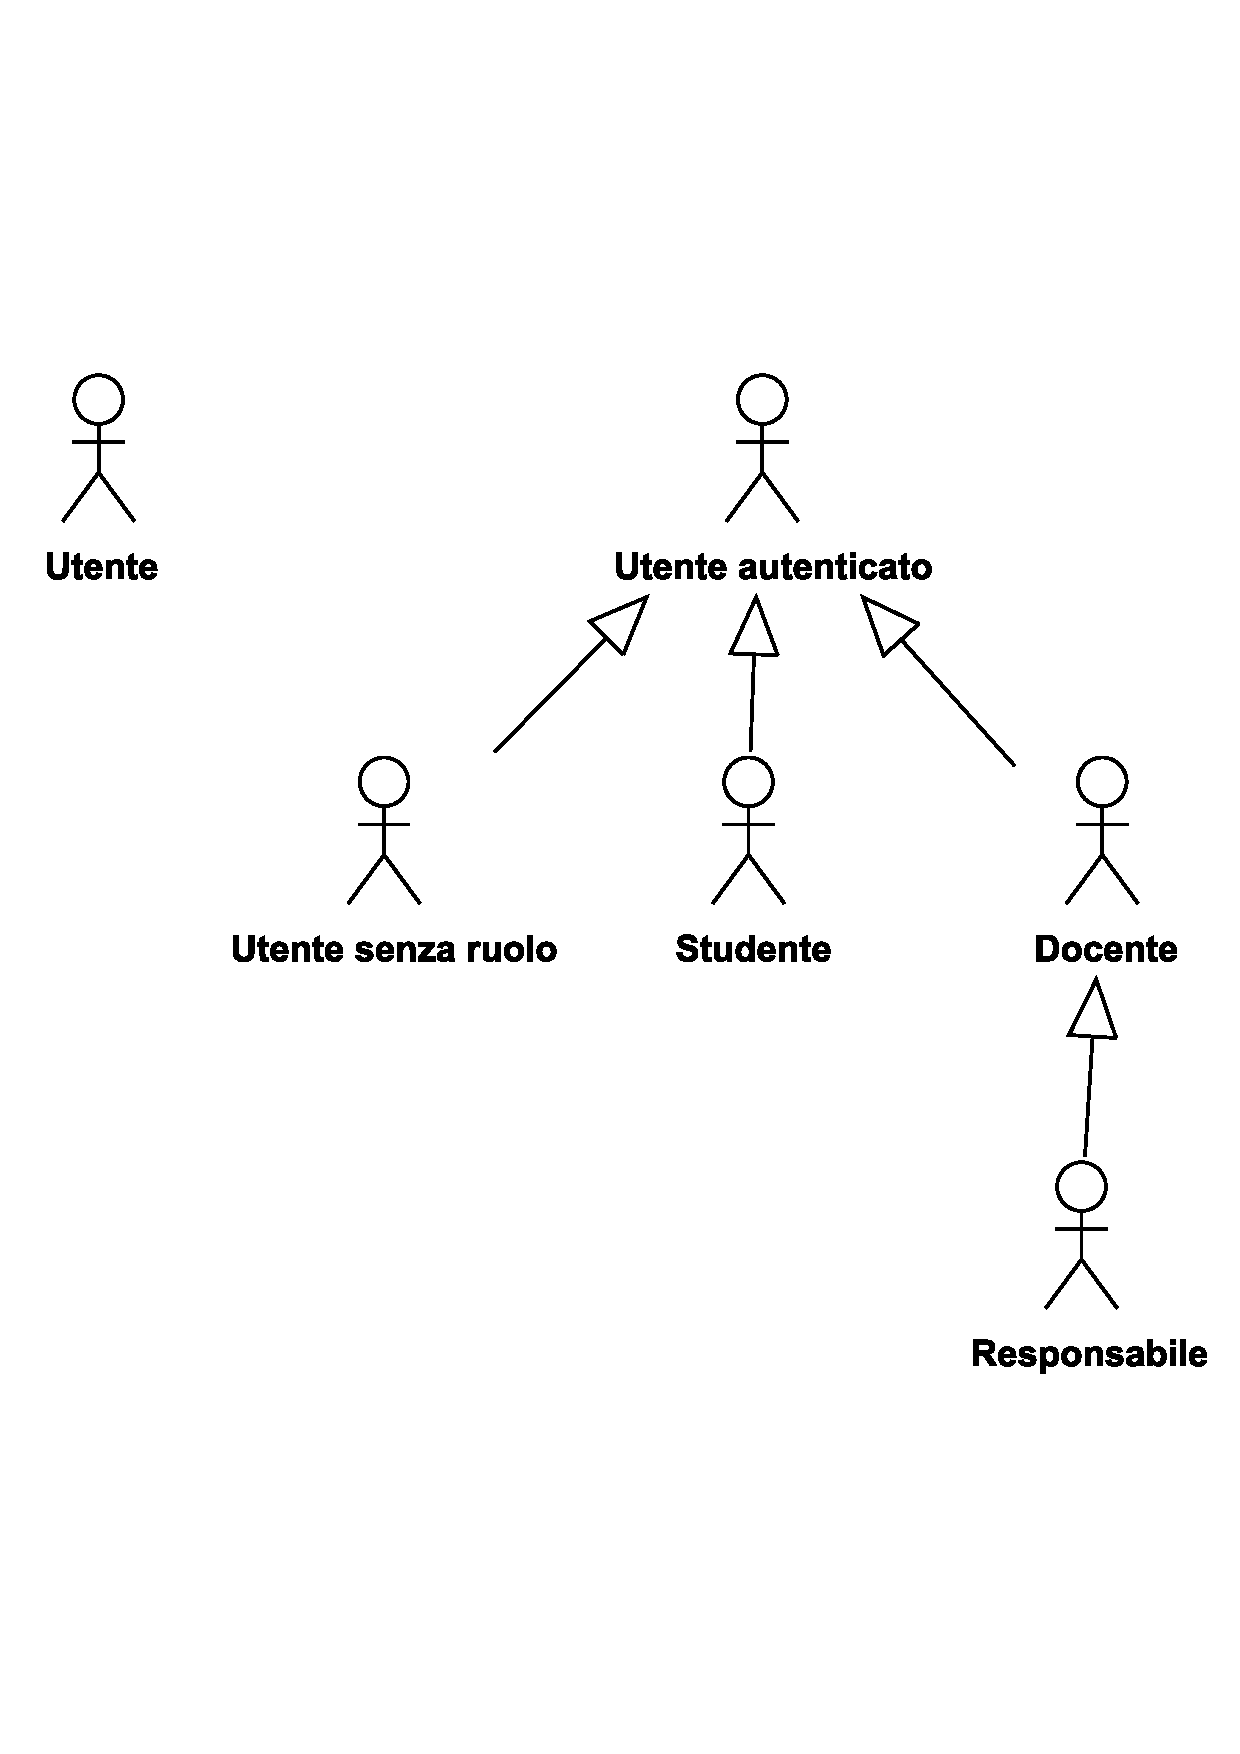
\includegraphics[scale=0.3]{Img/attori.pdf}}
	\caption{Gerarchia degli attori}
\end{figure}

Gli attori si dividono in:
\begin{itemize}

\item \bold{utente:} utente non registrato, o attore registrato ma non autenticato;
\item \bold{utente autenticato:} utente registrato che si è già autenticato;
\item \bold{utente senza ruolo:} utente autenticato a cui non è stato attribuito un ruolo (studente o docente);
\item \bold{studente:} utente autenticato a cui è stato attribuito il ruolo di studente;
\item \bold{docente:} utente autenticato a cui è stato attribuito il ruolo di docente;
\item \bold{responsabile:} utente con privilegi gestionali limitati a un singolo ente.
\end{itemize}

\subsection{Elenco dei casi d'uso}
I casi d'uso saranno descritti nel seguente modo: UC[id], con id=codice univoco. 

Per ogni caso d'uso saranno specificati:
\begin{itemize}
\item titolo;
\item attori coinvolti;
\item descrizione;
\item scenario principale;
\item scenari alternativi;
\item inclusioni;
\item estensioni;
\item generalizzazioni;
\item precondizione;
\item postcondizione.
\end{itemize}

\setcounter{secnumdepth}{0}
\setcounter{tocdepth}{0}

\subsubsection{UC1 Caso d'uso pubblico}
\begin{figure}[H]
\centering
\noindent\makebox[\textwidth]{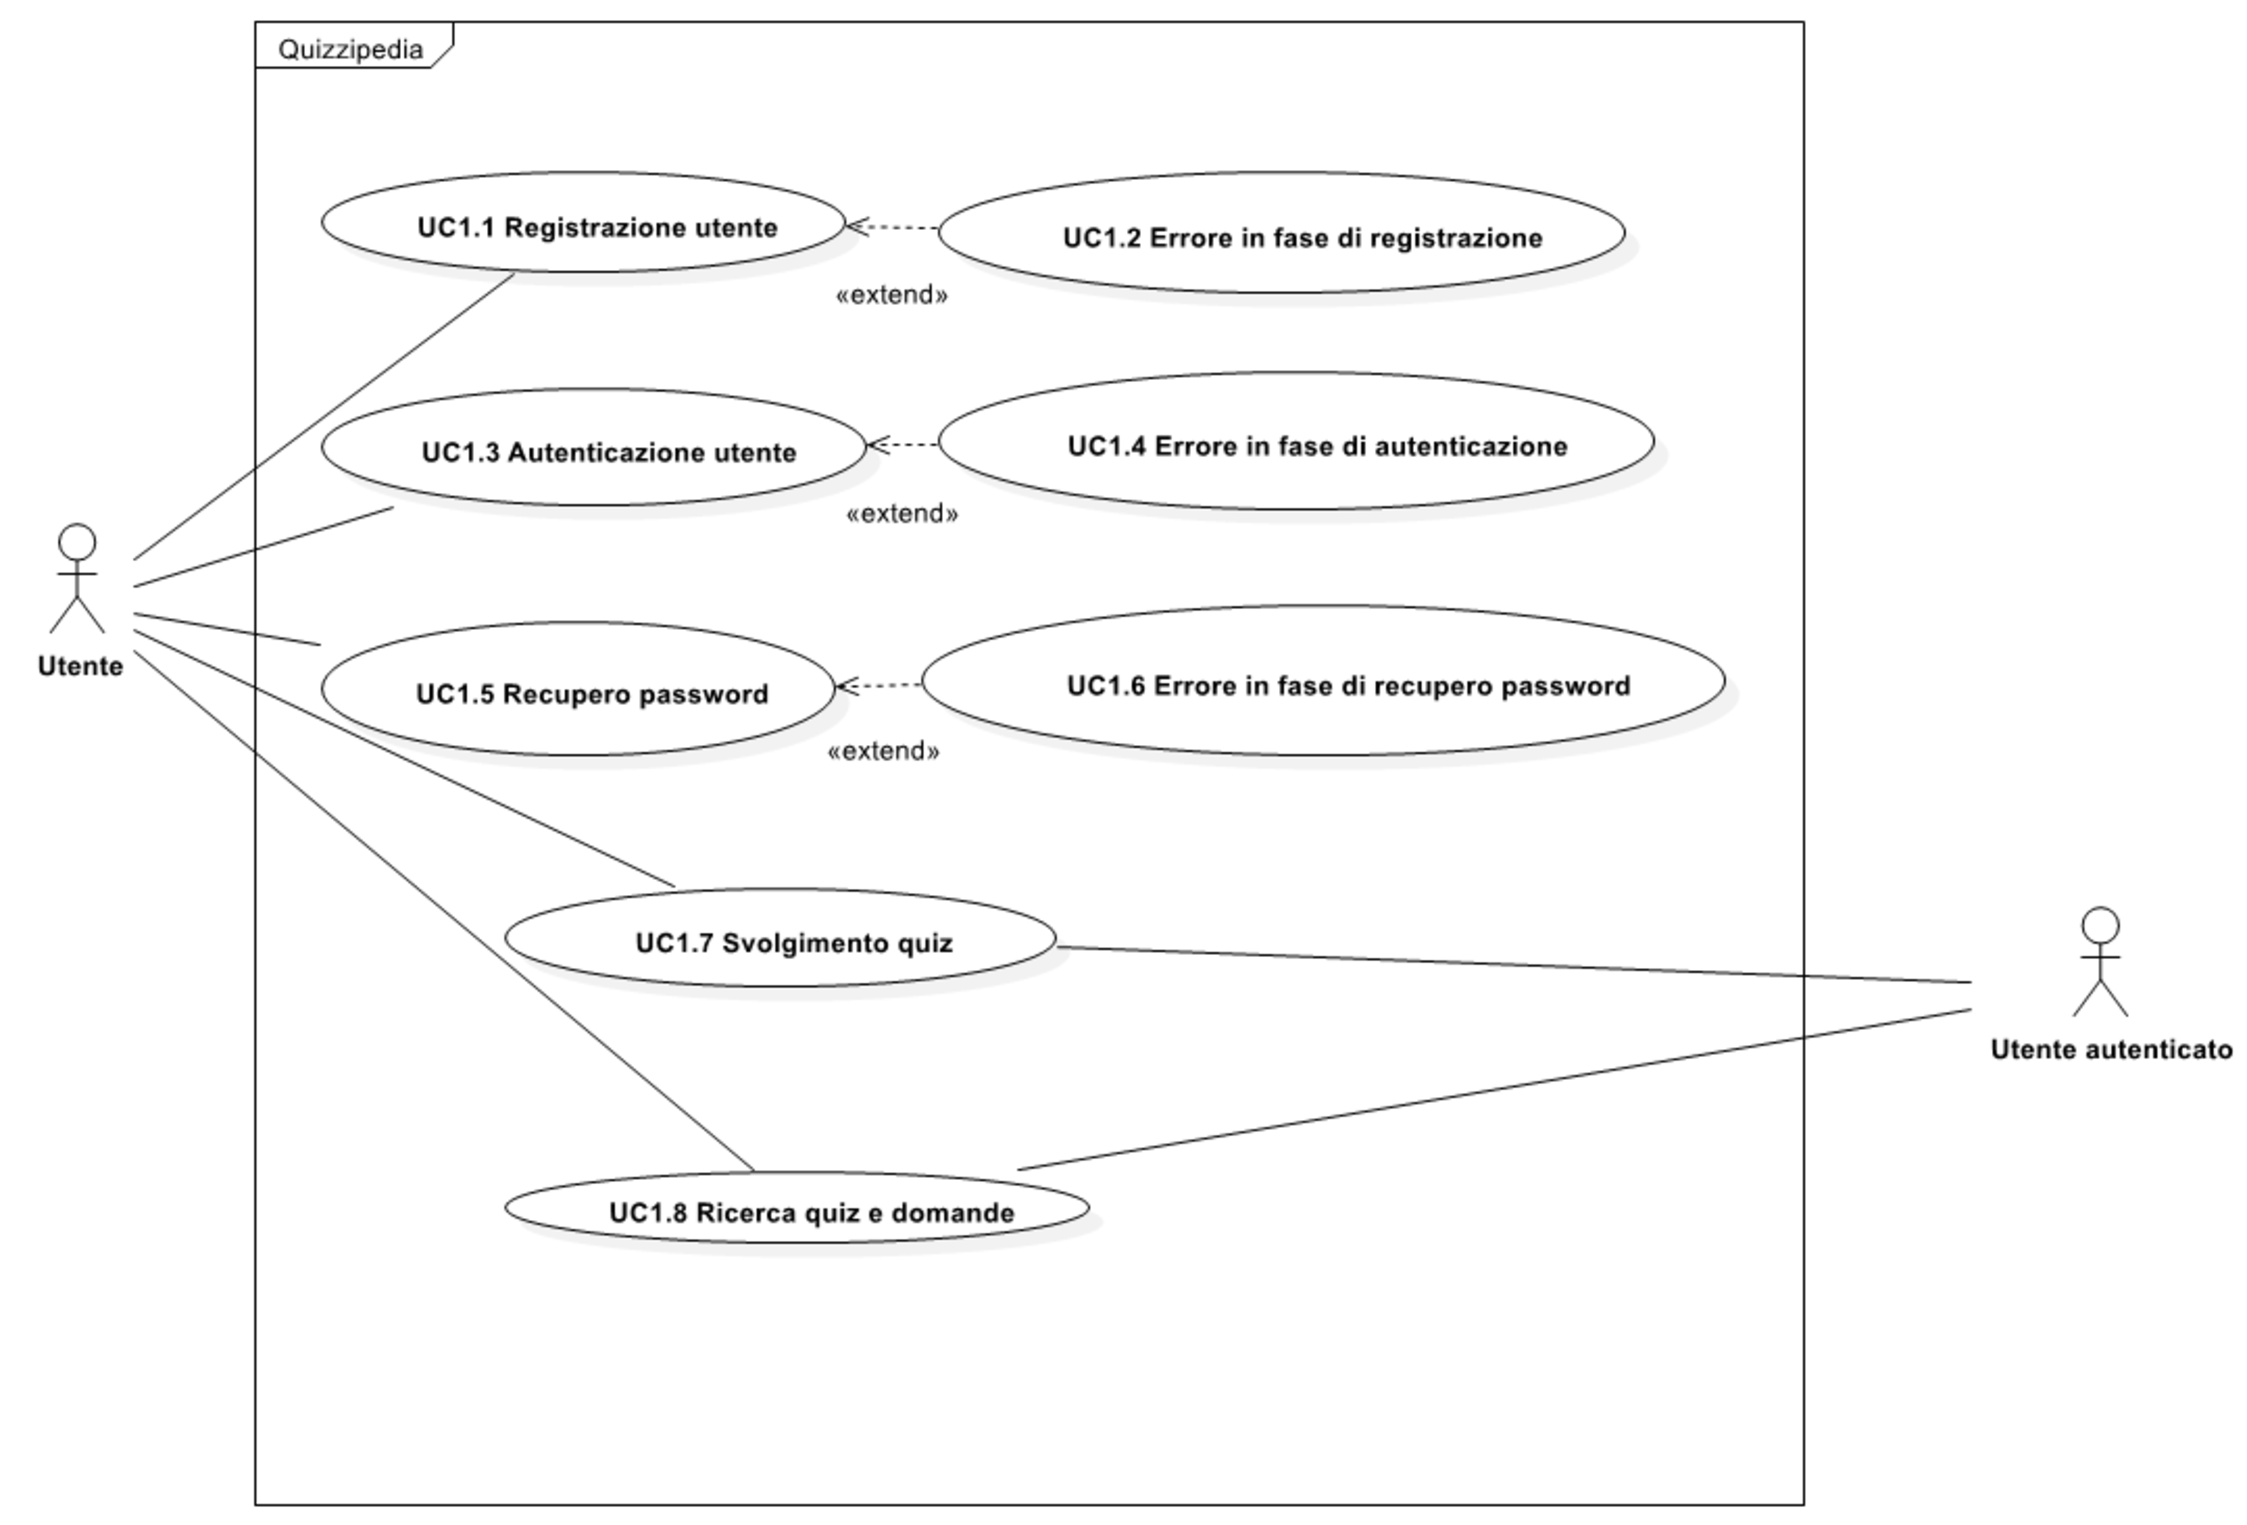
\includegraphics[width=\textwidth]{Img/UC Caso d'uso pubblico.pdf}}
\caption{UC1 Caso d'uso pubblico}
\end{figure}
\begin{itemize}
\item \textbf{Attori}: Utente, Utente Autenticato.
\item \textbf{Scenario principale}:
\begin{enumerate}
\item Registrazione utente (UC1.1);
\item Errore in fase di registrazione (UC1.2);
\item Autenticazione utente (UC1.3);
\item Errore in fase di autenticazione (UC1.4);
\item Recupero password (UC1.5);
\item Errore in fase di recupero password (UC1.6);
\item Svolgimento quiz (UC1.7);
\item Ricerca quiz e domande (UC1.8);
\item Interruzione volontaria della registrazione (UC1.9);
\item Interruzione volontaria dell'autenticazione (UC1.10);
\item Interruzione volontaria dello svolgimento del quiz (UC1.11);
\item Interruzione volontaria della ricerca (UC1.12);
\item Interruzione volontaria del recupero password (UC1.13).
\end{enumerate}
\item \textbf{Descrizione}: l'utente accede al sito. Può effettuare la registrazione, autenticarsi nel sistema, effettuare il recupero della propria password, cercare quiz e domande, svolgere quiz.
\item \textbf{Precondizione}: l'utente si è connesso al sito web di Quizzipedia attraverso un browser supportato.
\item \textbf{Postcondizione}: l'utente ha scelto l'operazione da intraprendere.
\end{itemize}
\subsubsection{UC1.1 Registrazione utente}
\begin{figure}[H]
\centering
\noindent\makebox[\textwidth]{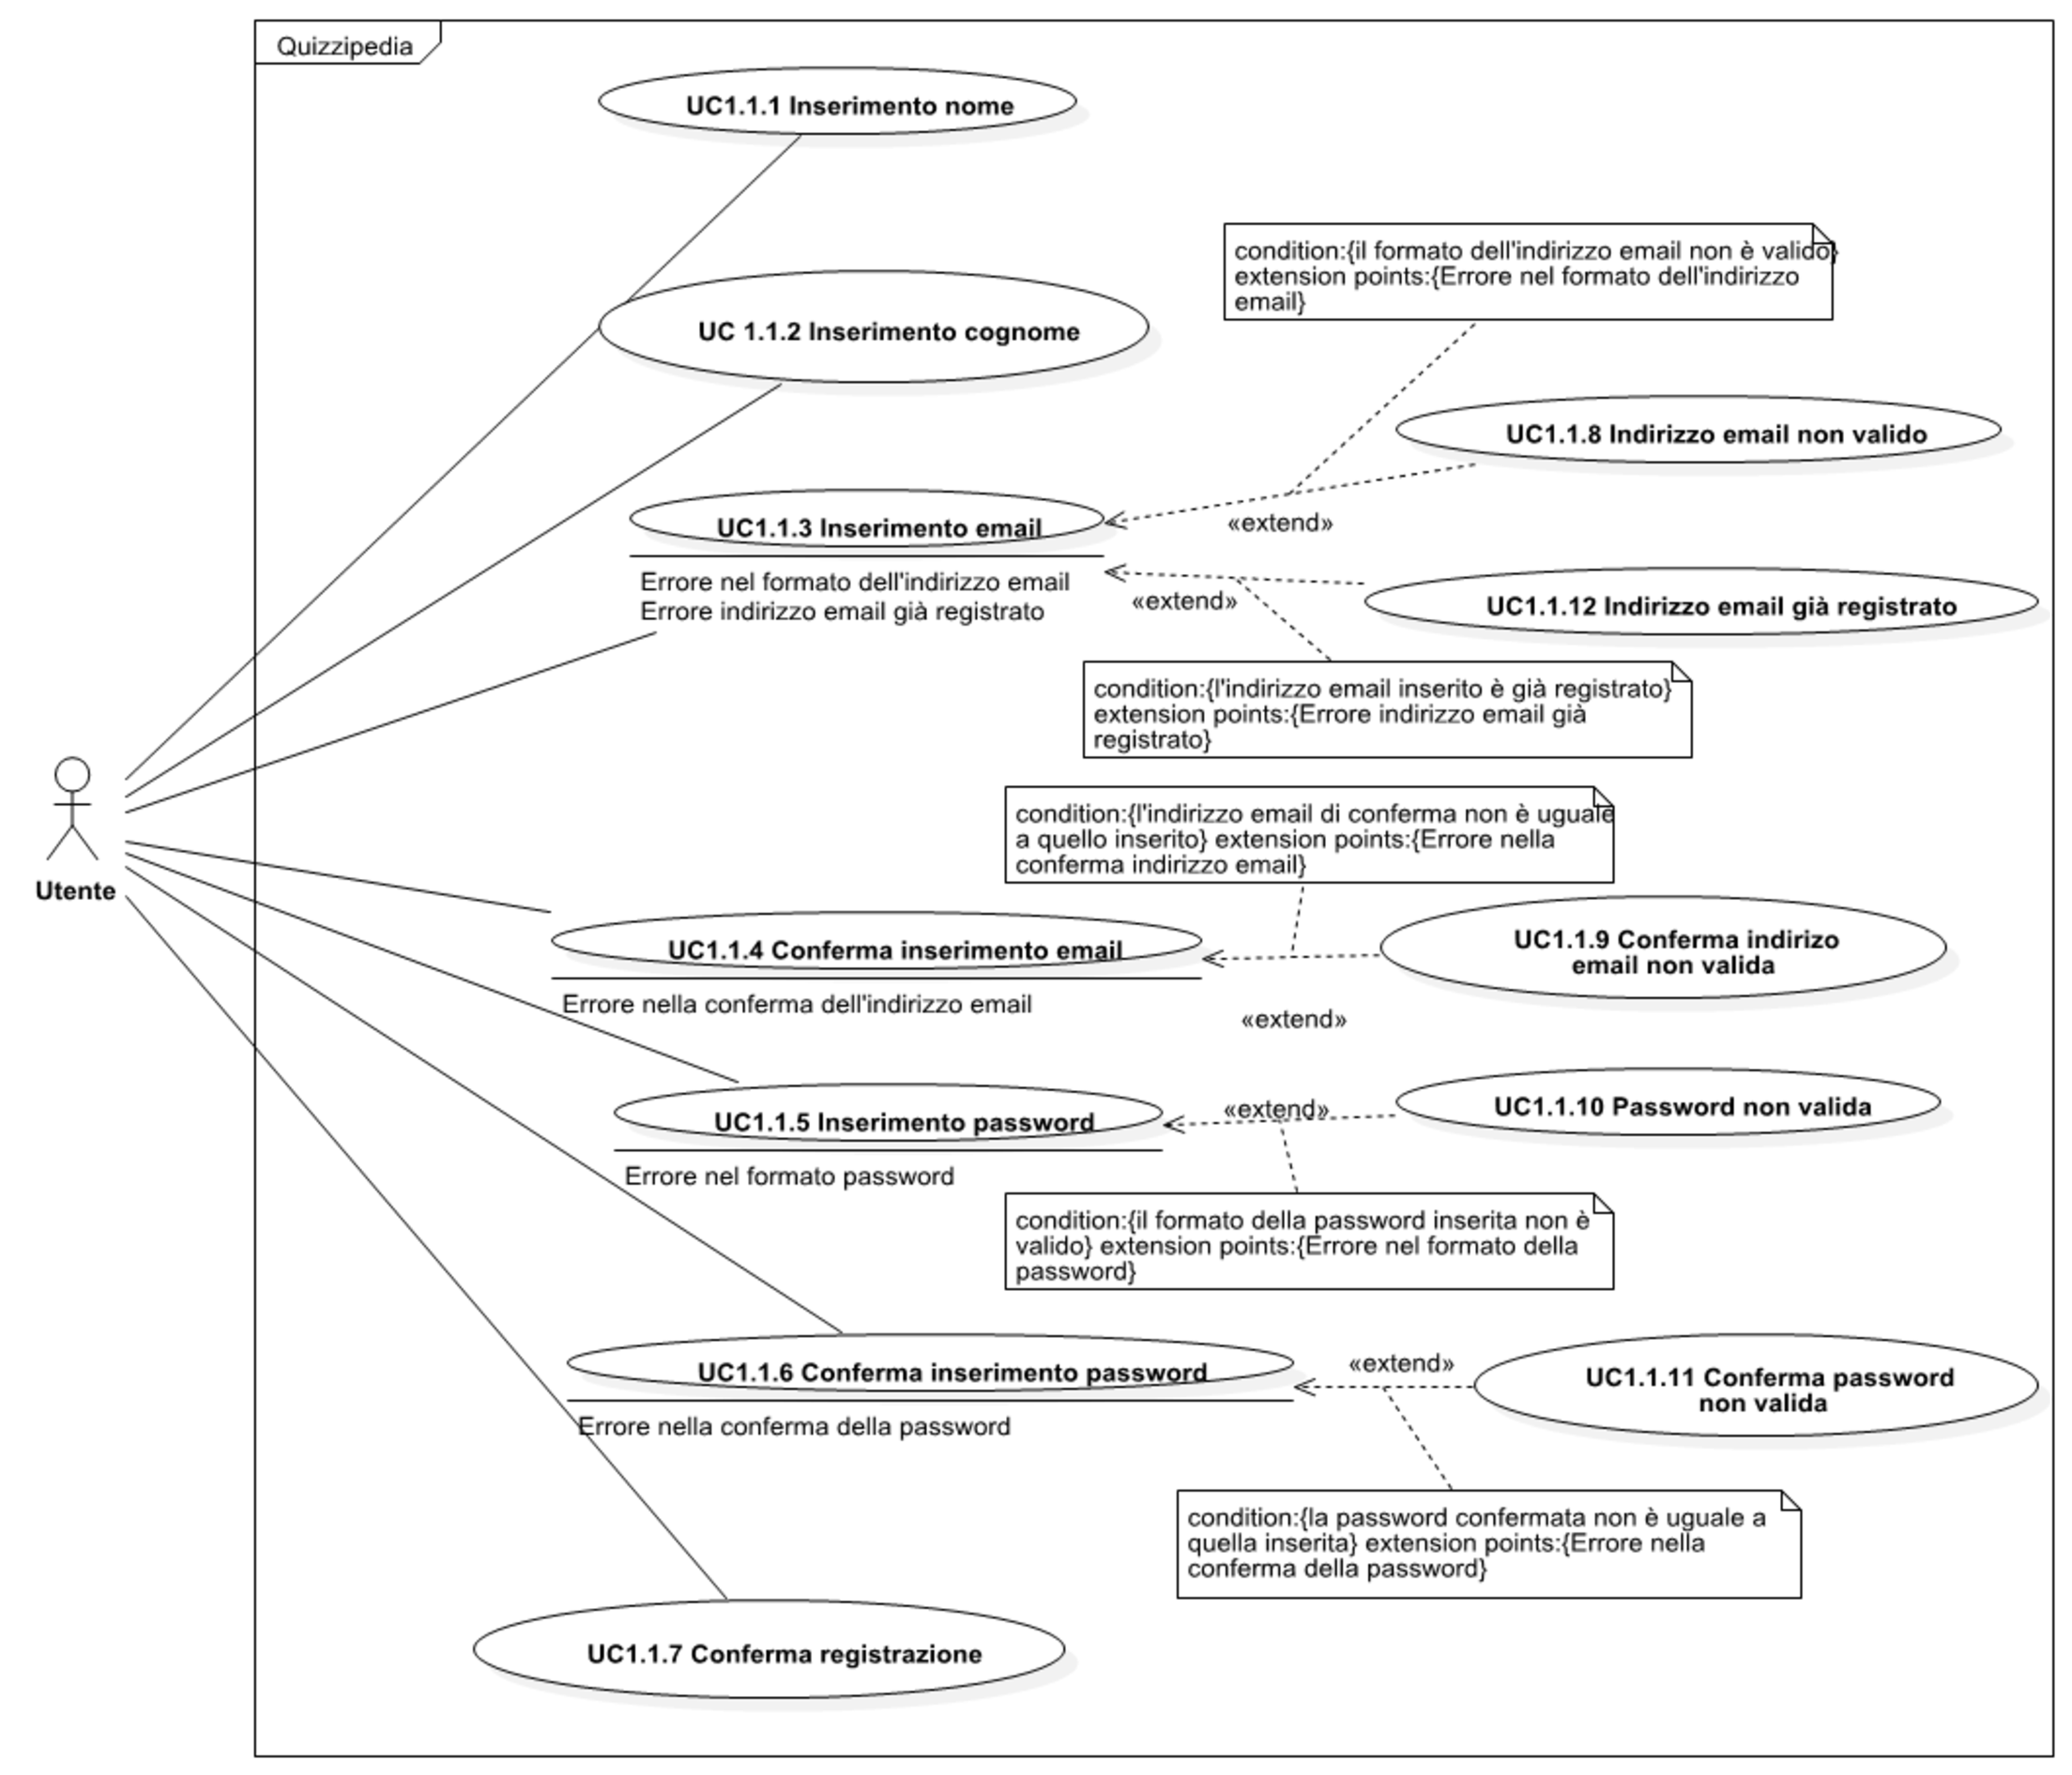
\includegraphics[width=\textwidth]{Img/UC Registrazione utente.pdf}}
\caption{UC1.1 Registrazione utente}
\end{figure}
\begin{itemize}
\item \textbf{Attori}: Utente.
\item \textbf{Scenario principale}:
\begin{enumerate}
\item Inserimento nome (UC1.1.1);
\item Inserimento cognome (UC1.1.2);
\item Inserimento email (UC1.1.3);
\item Conferma inserimento email (UC1.1.4);
\item Inserimento password (UC1.1.5);
\item Conferma inserimento password (UC1.1.6);
\item Conferma registrazione (UC1.1.7);
\item Indirizzo email non valido (UC1.1.8);
\item Conferma indirizzo email non valida (UC1.1.9);
\item Password non valida (UC1.1.10);
\item Conferma password non valida (UC1.1.11);
\item Indirizzo email già registrato (UC1.1.12).
\end{enumerate}
\item \textbf{Estensioni}:
\begin{itemize}
\item Errore in fase di registrazione (UC1.2);
\item Interruzione volontaria della registrazione (UC1.9).
\end{itemize}
\item \textbf{Descrizione}: l'utente crea un account Quizzipedia per poter usufruire delle funzionalità offerte dal sistema agli utenti registrati.
\item \textbf{Precondizione}: l'utente si è connesso al sito web di Quizzipedia attraverso un browser supportato e ha scelto di effettuare la registrazione.
\item \textbf{Postcondizione}: l'utente è stato registrato nel sistema con i dati immessi.
\end{itemize}
\subsubsection{UC1.1.1 Inserimento nome}
\begin{itemize}
\item \textbf{Attori}: Utente.
\item \textbf{Scenario principale}: l'utente inserisce il proprio nome.
\item \textbf{Descrizione}: per portare a termine la registrazione, l'utente deve inserire il proprio nome.
\item \textbf{Precondizione}: l'utente si trova nella pagina di registrazione e deve ancora inserire il proprio nome.
\item \textbf{Postcondizione}: l'utente ha inserito il nome.
\end{itemize}
\subsubsection{UC1.1.2 Inserimento cognome}
\begin{itemize}
\item \textbf{Attori}: Utente.
\item \textbf{Scenario principale}: l'utente inserisce il proprio cognome.
\item \textbf{Descrizione}: per portare a termine la registrazione, l'utente deve inserire il proprio cognome.
\item \textbf{Precondizione}: l'utente si trova nella pagina di registrazione e deve ancora inserire il proprio cognome.
\item \textbf{Postcondizione}: l'utente ha inserito il cognome.
\end{itemize}
\subsubsection{UC1.1.3 Inserimento email}
\begin{itemize}
\item \textbf{Attori}: Utente.
\item \textbf{Scenario principale}: l'utente inserisce il proprio indirizzo email.
\item \textbf{Estensioni}:
\begin{itemize}
\item Indirizzo email non valido (UC1.1.8).
\end{itemize}
\item \textbf{Descrizione}: per portare a termine la registrazione, l'utente deve inserire il proprio indirizzo email.
\item \textbf{Precondizione}: l'utente si trova nella pagina di registrazione e deve ancora inserire l'indirizzo email.
\item \textbf{Postcondizione}: l'utente ha inserito un indirizzo email valido.
\end{itemize}
\subsubsection{UC1.1.4 Conferma inserimento email}
\begin{itemize}
\item \textbf{Attori}: Utente.
\item \textbf{Scenario principale}: l'utente conferma l'inserimento del proprio indirizzo email.
\item \textbf{Estensioni}:
\begin{itemize}
\item Conferma indirizzo email non valida (UC1.1.9).
\end{itemize}
\item \textbf{Descrizione}: per portare a termine la registrazione, l'utente deve confermare il proprio indirizzo email.
\item \textbf{Precondizione}: l'utente si trova nella pagina di registrazione, ha inserito l'indirizzo email e deve ancora confermarlo.
\item \textbf{Postcondizione}: l'utente ha confermato un indirizzo email valido e uguale a quello inserito.
\end{itemize}
\subsubsection{UC1.1.5 Inserimento password}
\begin{itemize}
\item \textbf{Attori}: Utente.
\item \textbf{Scenario principale}: l'utente inserisce la propria password.
\item \textbf{Estensioni}:
\begin{itemize}
\item Password non valida (UC1.1.10).
\end{itemize}
\item \textbf{Descrizione}: per portare a termine la registrazione, l'utente deve inserire la propria password.
\item \textbf{Precondizione}: l'utente si trova nella pagina di registrazione e deve ancora inserire la password.
\item \textbf{Postcondizione}: l'utente ha inserito una password valida.
\end{itemize}
\subsubsection{UC1.1.6 Conferma inserimento password}
\begin{itemize}
\item \textbf{Attori}: Utente.
\item \textbf{Scenario principale}: l'utente conferma l'inserimento della propria password.
\item \textbf{Estensioni}:
\begin{itemize}
\item Conferma password non valida (UC1.1.11).
\end{itemize}
\item \textbf{Descrizione}: per portare a termine la registrazione, l'utente deve confermare la propria password.
\item \textbf{Precondizione}: l'utente si trova nella pagina di registrazione, ha inserito la password e deve ancora confermarla.
\item \textbf{Postcondizione}: l'utente ha confermato una password valida e uguale a quella inserita.
\end{itemize}
\subsubsection{UC1.1.7 Conferma registrazione}
\begin{itemize}
\item \textbf{Attori}: Utente.
\item \textbf{Scenario principale}: l'utente conferma la registrazione.
\item \textbf{Descrizione}: per portare a termine la registrazione, l'utente deve confermare i dati precedentemente inseriti.
\item \textbf{Precondizione}: l'utente si trova in una pagina del sito web che gli permette di confermare i dati precedentemente inseriti.
\item \textbf{Postcondizione}: L'utente ha scelto di continuare la registrazione con i dati immessi.
\end{itemize}
\subsubsection{UC1.1.8 Indirizzo email non valido}
\begin{itemize}
\item \textbf{Attori}: Utente.
\item \textbf{Scenario principale}: l'utente inserisce nuovamente l'indirizzo email.
\item \textbf{Descrizione}: l'indirizzo email non è valido e deve essere inserito nuovamente.
\item \textbf{Precondizione}: L'utente sta effettuando la registrazione e ha inserito un indirizzo email non valido.
\item \textbf{Postcondizione}: L'utente ha visualizzato un messaggio di errore che indica che l'indirizzo email inserito non è valido.
\end{itemize}
\subsubsection{UC1.1.9 Conferma indirizzo email non valida}
\begin{itemize}
\item \textbf{Attori}: Utente.
\item \textbf{Scenario principale}: l'utente conferma nuovamente l'indirizzo email.
\item \textbf{Descrizione}: l'indirizzo email non è uguale a quello precedentemente inserito.
\item \textbf{Precondizione}: L'utente sta effettuando la registrazione e ha confermato l'indirizzo email in modo errato.
\item \textbf{Postcondizione}: L'utente ha visualizzato un messaggio di errore che indica che l'indirizzo email confermato non è uguale a quello precedentemente inserito.
\end{itemize}
\subsubsection{UC1.1.10 Password non valida}
\begin{itemize}
\item \textbf{Attori}: Utente.
\item \textbf{Scenario principale}: l'utente inserisce nuovamente la password.
\item \textbf{Descrizione}: la password inserita non è valida e quindi deve essere inserita nuovamente.
\item \textbf{Precondizione}: l'utente si trova nella pagina di registrazione e ha inserito una password non valida.
\item \textbf{Postcondizione}: l'utente ha visualizzato un messaggio di errore che indica che la password inserita non è valida.
\end{itemize}
\subsubsection{UC1.1.11 Conferma password non valida}
\begin{itemize}
\item \textbf{Attori}: Utente.
\item \textbf{Scenario principale}: l'utente conferma la password nuovamente.
\item \textbf{Descrizione}: la password non è uguale a quella precedentemente inserita.
\item \textbf{Precondizione}: l'utente si trova nella pagina di registrazione e ha confermato la password in maniera errata.
\item \textbf{Postcondizione}: l'utente ha visualizzato un messaggio di errore che indica che la password confermata non è uguale a quella precedentemente inserita.
\end{itemize}
\subsubsection{UC1.1.12 Indirizzo email già registrato}
\begin{itemize}
\item \textbf{Attori}: Utente.
\item \textbf{Scenario principale}: l'utente inserisce nuovamente l'indirizzo email.
\item \textbf{Descrizione}: l'indirizzo email inserito è già registrato.
\item \textbf{Precondizione}: l'utente sta effettuando la registrazione e ha inserito un indirizzo email già registrato.
\item \textbf{Postcondizione}: L'utente ha visualizzato un messaggio di errore che indica che l'indirizzo email inserito è già registrato.
\end{itemize}
\subsubsection{UC1.2 Errore in fase di registrazione}
\begin{itemize}
\item \textbf{Attori}: Utente.
\item \textbf{Scenario principale}: l'utente visualizza il messaggio di errore.
\item \textbf{Descrizione}: l'utente visualizza un messaggio di errore che lo avvisa che il tentativo di autenticazione non è andato a buon termine.
\item \textbf{Precondizione}: si è verificata una delle seguenti condizioni: l'indirizzo email inserito non è associato a un account registrato, oppure la combinazione di indirizzo email e password immessa è errata.
\item \textbf{Postcondizione}: l'utente ha visualizzato il messaggio di errore.
\end{itemize}
\subsubsection{UC1.3 Autenticazione utente}
\begin{figure}[H]
\centering
\noindent\makebox[\textwidth]{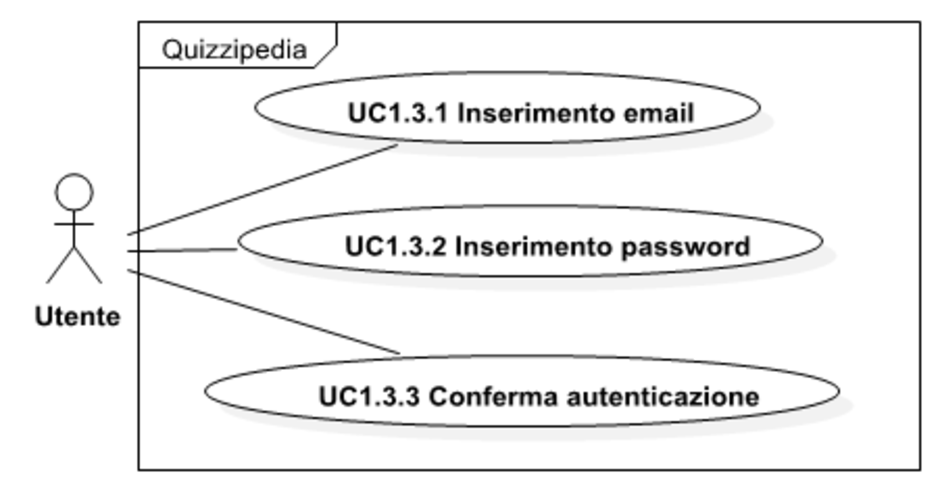
\includegraphics[width=\textwidth]{Img/UC Autenticazione utente.pdf}}
\caption{UC1.3 Autenticazione utente}
\end{figure}
\begin{itemize}
\item \textbf{Attori}: Utente.
\item \textbf{Scenario principale}:
\begin{enumerate}
\item Inserimento email (UC1.3.1);
\item Inserimento password (UC1.3.2);
\item Conferma autenticazione (UC1.3.3).
\end{enumerate}
\item \textbf{Estensioni}:
\begin{itemize}
\item Errore in fase di autenticazione (UC1.4);
\item Interruzione volontaria dell'autenticazione (UC1.10).
\end{itemize}
\item \textbf{Descrizione}: l'utente, se in possesso di un account Quizzipedia, deve avere la possibilità di autenticarsi.
\item \textbf{Precondizione}: l'utente si è connesso al sito web di Quizzipedia attraverso un browser supportato e ha scelto di effettuare l'autenticazione.
\item \textbf{Postcondizione}: il sistema ha autenticato l'utente.
\end{itemize}
\subsubsection{UC1.3.1 Inserimento email}
\begin{itemize}
\item \textbf{Attori}: Utente.
\item \textbf{Scenario principale}: l'utente inserisce il proprio indirizzo email.
\item \textbf{Descrizione}: per portare a termine l'autenticazione, l'utente deve inserire il proprio indirizzo email.
\item \textbf{Precondizione}: l'utente si trova in una pagina di autenticazione e deve ancora inserire il proprio indirizzo email.
\item \textbf{Postcondizione}: l'utente ha inserito il proprio indirizzo email.
\end{itemize}
\subsubsection{UC1.3.2 Inserimento password}
\begin{itemize}
\item \textbf{Attori}: Utente.
\item \textbf{Scenario principale}: l'utente inserisce la propria password.
\item \textbf{Descrizione}: per portare a termine l'autenticazione, l'utente deve inserire la password.
\item \textbf{Precondizione}: l'utente si trova in una pagina di autenticazione e deve ancora inserire la password.
\item \textbf{Postcondizione}: l'utente ha inserito la password.
\end{itemize}
\subsubsection{UC1.3.3 Conferma autenticazione}
\begin{itemize}
\item \textbf{Attori}: Utente.
\item \textbf{Scenario principale}: l'utente conferma l'autenticazione.
\item \textbf{Descrizione}: per portare a termine l'autenticazione, l'utente deve confermare l'autenticazione con l'indirizzo email e  la password immessi.
\item \textbf{Precondizione}: l'utente si trova in una pagina del sito web che gli permette di confermare l'autenticazione.
\item \textbf{Postcondizione}: l'utente ha scelto di continuare l'autenticazione con i dati immessi.
\end{itemize}
\subsubsection{UC1.4 Errore in fase di autenticazione}
\begin{itemize}
\item \textbf{Attori}: Utente.
\item \textbf{Scenario principale}: l'utente visualizza il messaggio di errore.
\item \textbf{Descrizione}: si è verificata una delle seguenti condizioni: l'indirizzo email inserito non è associato a un account registrato, oppure la combinazione di indirizzo email e password immessa è errata.
\item \textbf{Precondizione}: l'utente ha effettuato un tentativo di autenticazione che non è andato a buon termine.
\item \textbf{Postcondizione}: l'utente ha visualizzato il messaggio di errore.
\end{itemize}
\subsubsection{UC1.5 Recupero password}
\begin{figure}[H]
\centering
\noindent\makebox[\textwidth]{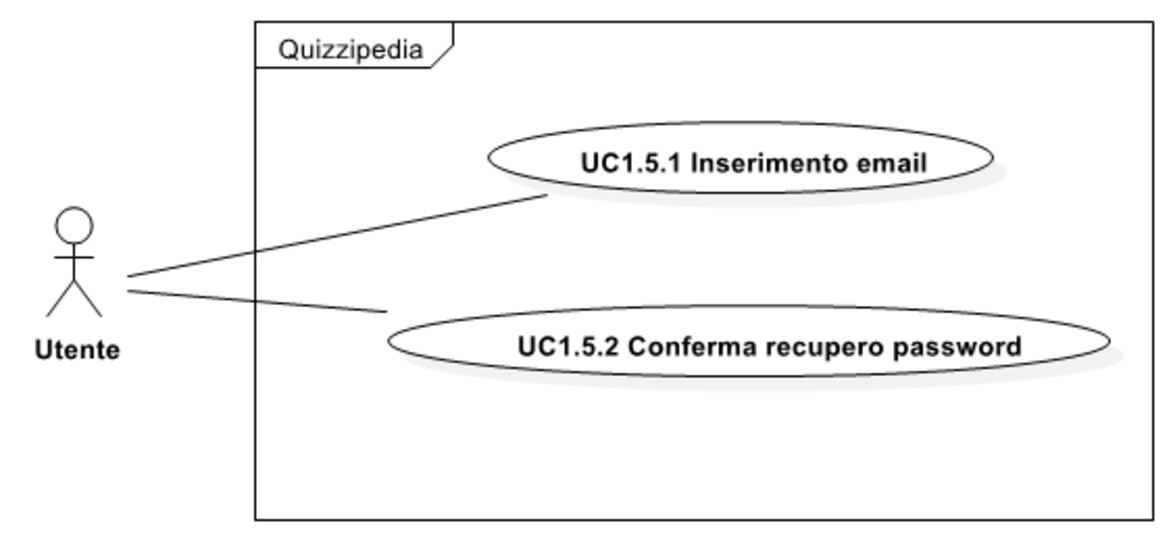
\includegraphics[width=\textwidth]{Img/UC Recupero password.pdf}}
\caption{UC1.5 Recupero password}
\end{figure}
\begin{itemize}
\item \textbf{Attori}: Utente.
\item \textbf{Scenario principale}:
\begin{enumerate}
\item Inserimento email (UC1.5.1);
\item Conferma recupero password (UC1.5.2).
\end{enumerate}
\item \textbf{Estensioni}:
\begin{itemize}
\item Errore in fase di recupero password (UC1.6);
\item Interruzione volontaria del recupero password (UC1.13).
\end{itemize}
\item \textbf{Descrizione}: l’utente in possesso di un account Quizzipedia deve avere la possibilità di accedere al sistema anche in caso di dimenticanza della propria password, a patto che ricordi l’indirizzo email a cui è associato il suo account.
\item \textbf{Precondizione}: l'utente si è connesso al sito web di Quizzipedia attraverso un browser supportato e vuole recuperare l‘accesso al proprio account Quizzipedia.
\item \textbf{Postcondizione}: l’utente ha recuperato l’accesso al proprio account Quizzipedia.
\end{itemize}
\subsubsection{UC1.5.1 Inserimento email}
\begin{itemize}
\item \textbf{Attori}: Utente.
\item \textbf{Scenario principale}: l'utente inserisce il suo indirizzo email.
\item \textbf{Descrizione}: per portare a termine l'operazione, l'utente deve inserire il proprio indirizzo email. Se l'indirizzo email è associato a un account registrato, gli verrà inviata una password temporanea o un link che consentirà all'utente di scegliere una nuova password senza dover ricordare la vecchia.
\item \textbf{Precondizione}: l'utente si trova nella pagina di recupero password e deve ancora inserire l'indirizzo email.
\item \textbf{Postcondizione}: l'utente ha inserito il proprio indirizzo email.
\end{itemize}
\subsubsection{UC1.5.2 Conferma recupero password}
\begin{itemize}
\item \textbf{Attori}: Utente.
\item \textbf{Scenario principale}: l'utente conferma il recupero della password.
\item \textbf{Descrizione}: per portare a termine il recupero password, l'utente deve confermare l'operazione con l'indirizzo email immesso.
\item \textbf{Precondizione}: l'utente si trova in una pagina del sito web che gli permette di confermare il recupero password.
\item \textbf{Postcondizione}: l'utente ha scelto di continuare il recupero password con l'indirizzo email immesso.
\end{itemize}
\subsubsection{UC1.6 Errore in fase di recupero password}
\begin{itemize}
\item \textbf{Attori}: Utente.
\item \textbf{Scenario principale}: l'utente visualizza il messaggio di errore.
\item \textbf{Descrizione}: l'utente visualizza un messaggio di errore che lo avvisa che il tentativo di recupero password non è andato a buon termine.
\item \textbf{Precondizione}: si è verificata la seguente condizione: l'indirizzo email inserito non è associato a un account registrato.
\item \textbf{Postcondizione}: l'utente ha visualizzato il messaggio di errore.
\end{itemize}
\subsubsection{UC1.7 Svolgimento quiz}
\begin{figure}[H]
\centering
\noindent\makebox[\textwidth]{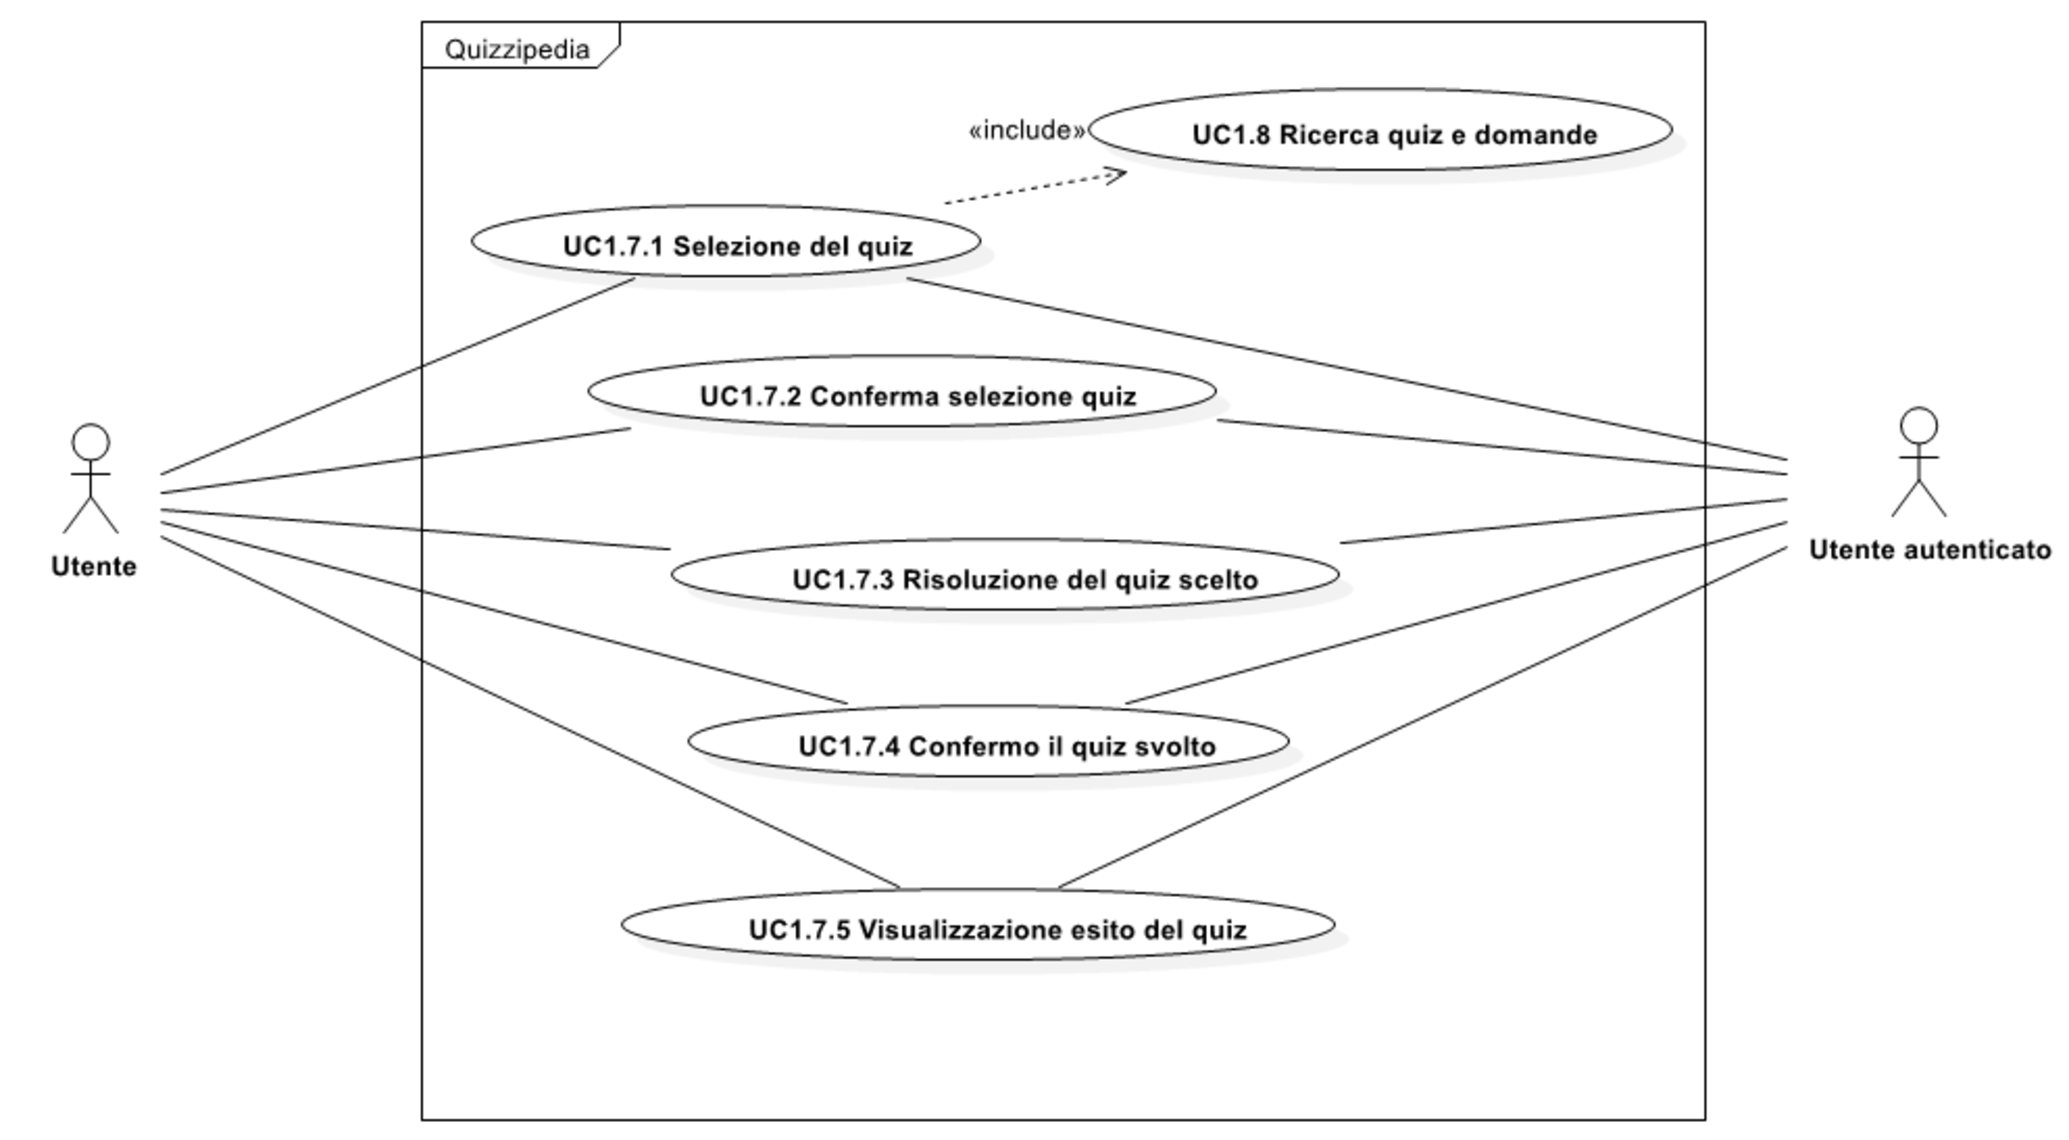
\includegraphics[width=\textwidth]{Img/UC Svolgimento quiz.pdf}}
\caption{UC1.7 Svolgimento quiz}
\end{figure}
\begin{itemize}
\item \textbf{Attori}: Utente, Utente Autenticato.
\item \textbf{Scenario principale}:
\begin{enumerate}
\item Selezione quiz (UC1.7.1);
\item Conferma selezione quiz (UC1.7.2);
\item Risoluzione quiz scelto (UC1.7.3);
\item Conferma risoluzione quiz (UC1.7.4);
\item Visualizzazione esito del quiz (UC1.7.5).
\end{enumerate}
\item \textbf{Estensioni}:
\begin{itemize}
\item Interruzione volontaria dello svolgimento del quiz (UC1.11).
\end{itemize}
\item \textbf{Descrizione}: l'utente deve poter svolgere un quiz conforme ai permessi dell'utente.
\item \textbf{Precondizione}: l'utente è autenticato nel sistema.
\item \textbf{Postcondizione}: l'utente ha finito di svolgere un quiz.
\end{itemize}
\subsubsection{UC1.7.1 Selezione quiz}
\begin{itemize}
\item \textbf{Attori}: Utente, Utente Autenticato.
\item \textbf{Scenario principale}: l'utente seleziona il quiz da svolgere.
\item \textbf{Descrizione}: l'utente deve poter selezionare il quiz che intende svolgere.
\item \textbf{Precondizione}: l'utente ha scelto di svolgere un quiz e vuole selezionarne uno.
\item \textbf{Postcondizione}: l'utente ha selezionato il quiz.
\end{itemize}
\subsubsection{UC1.7.2 Conferma selezione quiz}
\begin{itemize}
\item \textbf{Attori}: Utente, Utente Autenticato.
\item \textbf{Scenario principale}: l'utente conferma la selezione del quiz.
\item \textbf{Descrizione}: l'utente deve confermare la selezione del quiz scelto per iniziarne lo svolgimento.
\item \textbf{Precondizione}: l'utente ha selezionato il quiz da svolgere e deve confermarlo.
\item \textbf{Postcondizione}: l'utente ha confermato la selezione del quiz.
\end{itemize}
\subsubsection{UC1.7.3 Risoluzione quiz scelto}
\begin{itemize}
\item \textbf{Attori}: Utente, Utente Autenticato.
\item \textbf{Scenario principale}: l'utente risolve il quiz scelto.
\item \textbf{Descrizione}: l'utente deve poter svolgere il quiz che ha selezionato, una domanda alla volta. È possibile spostarsi a piacimento fra le domande e rispondere a una domanda più volte, l'ultima risposta sovrascrive le precedenti.
\item \textbf{Precondizione}: l'utente ha selezionato e confermato un quiz da svolgere.
\item \textbf{Postcondizione}: l'utente ha concluso la risoluzione del quiz.
\end{itemize}
\subsubsection{UC1.7.4 Conferma risoluzione quiz}
\begin{itemize}
\item \textbf{Attori}: Utente, Utente Autenticato.
\item \textbf{Scenario principale}: l'utente conferma la risoluzione del quiz.
\item \textbf{Descrizione}: l'utente deve poter confermare la risoluzione del quiz, terminandone così lo svolgimento. Una volta confermata la risoluzione non sarà più possibile modificare le risposte.
\item \textbf{Precondizione}:  l'utente ha terminato la risoluzione del quiz e vuole riceverne l'esito.
\item \textbf{Postcondizione}: l'utente ha confermato la risoluzione del quiz con le risposte date.
\end{itemize}
\subsubsection{UC1.7.5 Visualizzazione esito del quiz}
\begin{itemize}
\item \textbf{Attori}: Utente, Utente Autenticato.
\item \textbf{Scenario principale}: l'utente visualizza l'esito del quiz svolto.
\item \textbf{Descrizione}: l'utente deve poter visualizzare l'esito del quiz svolto. L'esito può comprendere: il voto ricevuto, la soluzione corretta delle domande a cui è stata data una risposta errata.
\item \textbf{Precondizione}: l'utente ha confermato la risoluzione del quiz svolto.
\item \textbf{Postcondizione}: l'utente ha visualizzato l'esito.
\end{itemize}
\subsubsection{UC1.8 Ricerca quiz e domande}
\begin{figure}[H]
\centering
\noindent\makebox[\textwidth]{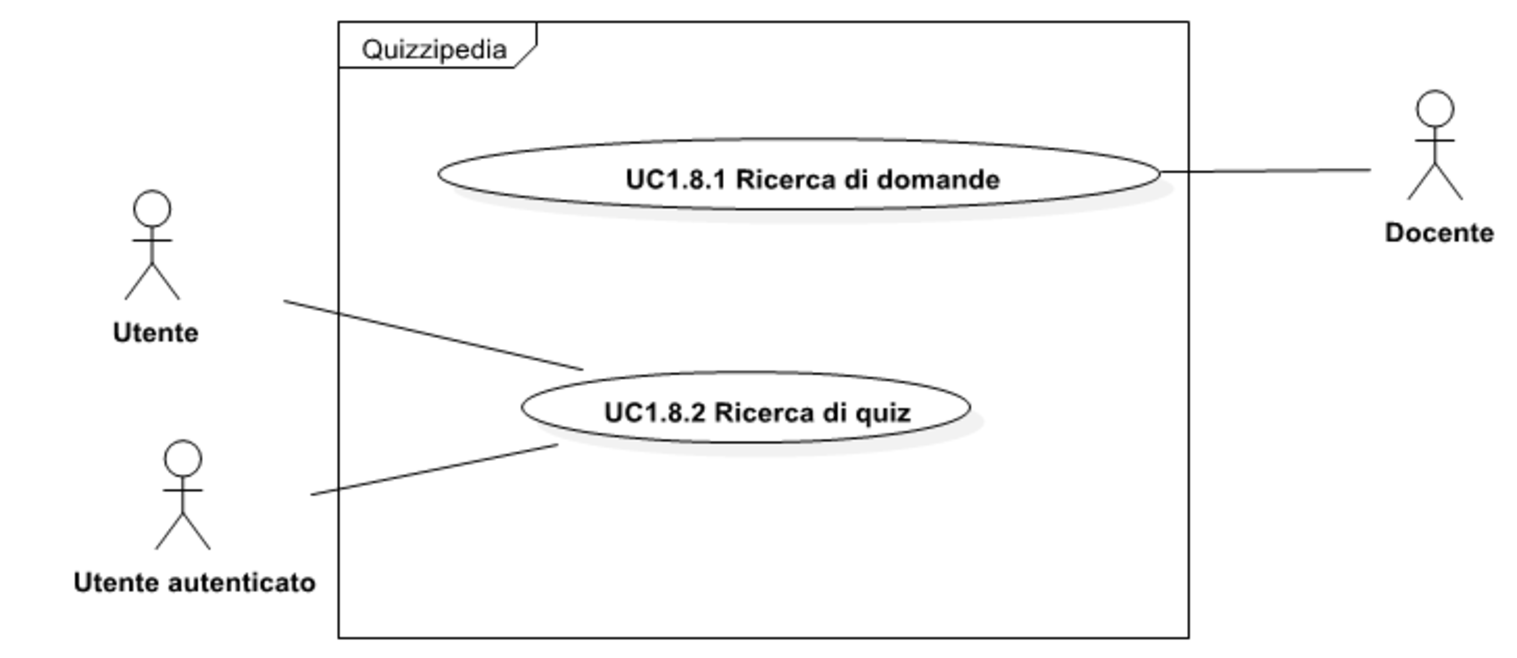
\includegraphics[width=\textwidth]{Img/UC Ricerca quiz e domande.pdf}}
\caption{UC1.8 Ricerca quiz e domande}
\end{figure}
\begin{itemize}
\item \textbf{Attori}: Utente, Utente Autenticato.
\item \textbf{Scenario principale}:
\begin{enumerate}
\item Selezione parametri di ricerca (UC1.8.1);
\item Conferma inizio ricerca (UC1.8.2);
\item Visualizzazione lista risultati (UC1.8.3).
\end{enumerate}
\item \textbf{Estensioni}:
\begin{itemize}
\item Interruzione volontaria della ricerca (UC1.12).
\end{itemize}
\item \textbf{Descrizione}: l'utente può effettuare una ricerca di quiz e domande presenti nel sistema. La ricerca è personalizzabile attraverso vari parametri di ricerca.
\item \textbf{Precondizione}: l'utente desidera effettuare una ricerca di quiz e domande.
\item \textbf{Postcondizione}: l'utente ha effettuato la ricerca.
\end{itemize}
\subsubsection{UC1.8.1 Selezione parametri di ricerca}
\begin{figure}[H]
\centering
\noindent\makebox[\textwidth]{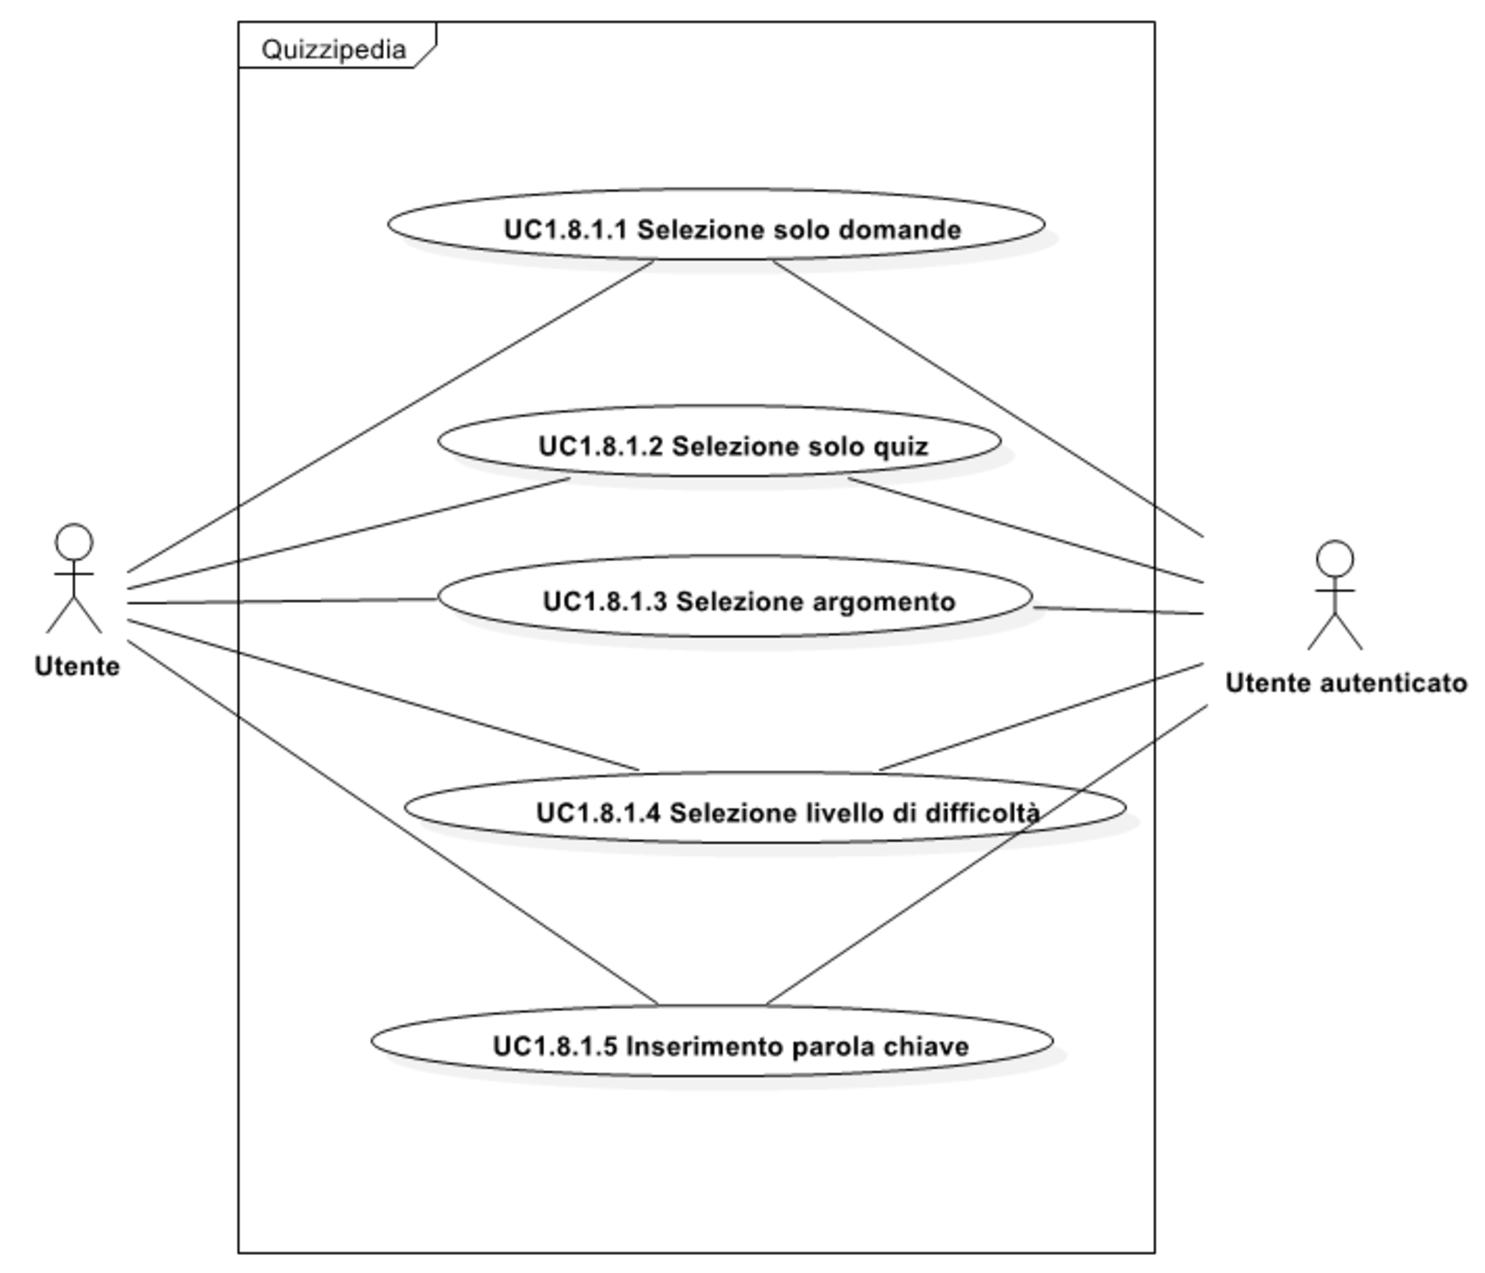
\includegraphics[width=\textwidth]{Img/UC Selezione parametri di ricerca.pdf}}
\caption{UC1.8.1 Selezione parametri di ricerca}
\end{figure}
\begin{itemize}
\item \textbf{Attori}: Utente, Utente Autenticato.
\item \textbf{Scenario principale}:
\begin{enumerate}
\item Selezione solo domande (UC1.8.1.1);
\item Selezione solo quiz (UC1.8.1.2);
\item Selezione argomenti nella ricerca (UC1.8.1.3);
\item Selezione livelli di difficoltà (UC1.8.1.4);
\item Selezione parole chiave (UC1.8.1.5).
\end{enumerate}
\item \textbf{Descrizione}: l’utente deve poter personalizzare la ricerca attraverso diversi parametri.
\item \textbf{Precondizione}: l’utente ha scelto di effettuare una ricerca.
\item \textbf{Postcondizione}: l’utente ha selezionato i parametri desiderati.
\end{itemize}
\subsubsection{UC1.8.1.1 Selezione solo domande}
\begin{itemize}
\item \textbf{Attori}: Utente, Utente Autenticato.
\item \textbf{Scenario principale}: l'utente seleziona/deseleziona l'opzione 'solo domande'.
\item \textbf{Descrizione}: l'utente deve poter selezionare/deselezionare l'opzione 'solo domande', che escluderà i quiz dalla ricerca. Se l'opzione 'solo quiz' è stata selezionata in precedenza, sarà deselezionata automaticamente.
\item \textbf{Precondizione}: l'utente sta personalizzando la ricerca attraverso dei parametri.
\item \textbf{Postcondizione}: l'utente ha selezionato/deselezionato il parametro 'solo domande'.
\end{itemize}
\subsubsection{UC1.8.1.2 Selezione solo quiz}
\begin{figure}[H]
\centering
\noindent\makebox[\textwidth]{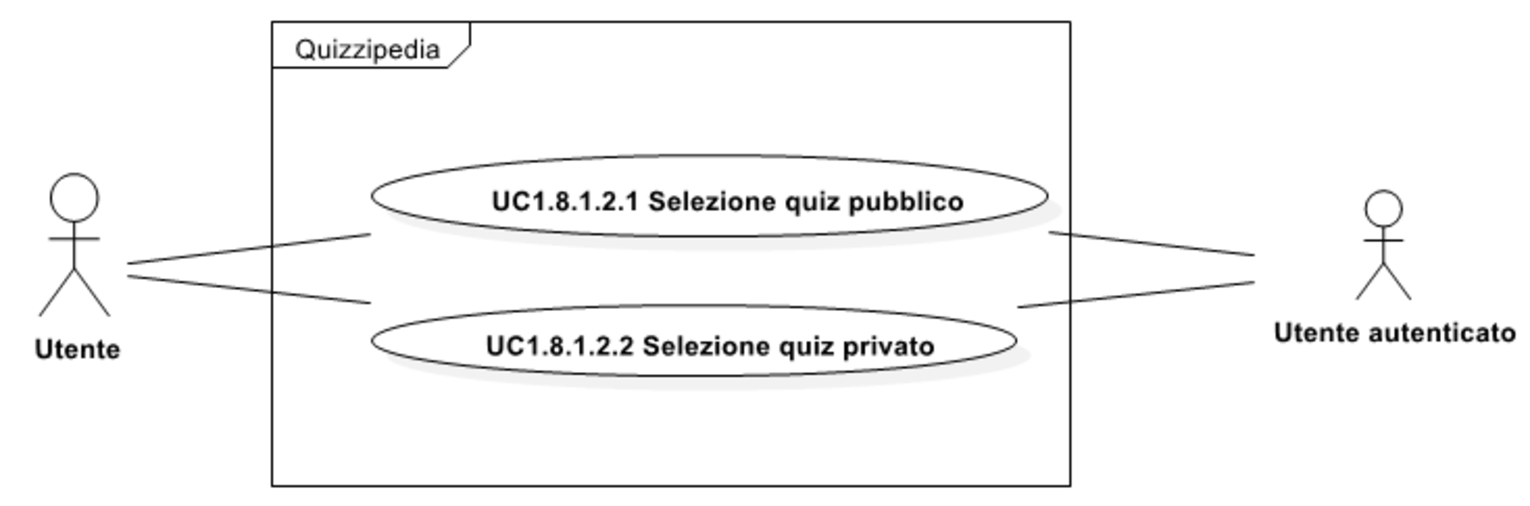
\includegraphics[width=\textwidth]{Img/UC Selezione solo quiz.pdf}}
\caption{UC1.8.1.2 Selezione solo quiz}
\end{figure}
\begin{itemize}
\item \textbf{Attori}: Utente, Utente Autenticato.
\item \textbf{Scenario principale}:
\begin{enumerate}
\item Selezione quiz pubblico (UC1.8.1.2.1);
\item Selezione quiz privato (UC1.8.1.2.2);
\item Errore permesso di accesso a quiz privati (UC1.8.1.2.3).
\end{enumerate}
\item \textbf{Descrizione}: l'utente deve poter selezionare/deselezionare l'opzione 'solo quiz', che escluderà le domande dalla ricerca. Se l'opzione 'solo domande' è stata selezionata in precedenza, sarà deselezionata automaticamente.
\item \textbf{Precondizione}: l'utente sta personalizzando la ricerca attraverso dei parametri.
\item \textbf{Postcondizione}: l'utente ha selezionato/deselezionato il parametro 'solo quiz'.
\end{itemize}
\subsubsection{UC1.8.1.2.1 Selezione quiz pubblico}
\begin{itemize}
\item \textbf{Attori}: Utente, Utente Autenticato.
\item \textbf{Scenario principale}: l'utente seleziona/deseleziona l'opzione 'quiz pubblico'.
\item \textbf{Descrizione}: l'utente deve poter selezionare/deselezionare l'opzione 'quiz pubblico', che escluderà dalla ricerca i quiz privati.
\item \textbf{Precondizione}: l'utente sta personalizzando la ricerca attraverso dei parametri.
\item \textbf{Postcondizione}: l'utente ha selezionato/deselezionato il parametro 'quiz pubblico'.
\end{itemize}
\subsubsection{UC1.8.1.2.2 Selezione quiz privato}
\begin{itemize}
\item \textbf{Attori}: Utente, Utente Autenticato.
\item \textbf{Scenario principale}: l'utente seleziona/deseleziona l'opzione 'quiz privato'.
\item \textbf{Descrizione}: l'utente deve poter selezionare/deselezionare l'opzione 'quiz privato', che escluderà dalla ricerca i quiz pubblici.
\item \textbf{Precondizione}: l'utente sta personalizzando la ricerca attraverso dei parametri.
\item \textbf{Postcondizione}: l'utente ha selezionato/deselezionato il parametro 'quiz privato'.
\end{itemize}
\subsubsection{UC1.8.1.2.3 Errore permesso di accesso a quiz privati}
\begin{itemize}
\item \textbf{Attori}: Utente, Utente Autenticato.
\item \textbf{Scenario principale}: l'utente visualizza il messagio di errore.
\item \textbf{Descrizione}: l'utente non ha il permesso di visualizzare quiz privati.
\item \textbf{Precondizione}: l'utente sta selezionando  quiz privati senza averne il permesso.
\item \textbf{Postcondizione}: l'utente ha visualizzato un messaggio di errore che indica che non ha il permesso di visualizzare quiz privati.
\end{itemize}
\subsubsection{UC1.8.1.3 Selezione argomenti nella ricerca}
\begin{itemize}
\item \textbf{Attori}: Utente, Utente Autenticato.
\item \textbf{Scenario principale}: l'utente seleziona/deseleziona gli argomenti.
\item \textbf{Descrizione}: l'utente deve poter selezionare/deselezionare uno o più argomenti, escludendo domande e quiz di argomenti non selezionati dalla ricerca.
\item \textbf{Precondizione}: l'utente sta personalizzando la ricerca attraverso dei parametri.
\item \textbf{Postcondizione}: l'utente ha selezionato/deselezionato gli argomenti.
\end{itemize}
\subsubsection{UC1.8.1.4 Selezione livelli di difficoltà}
\begin{itemize}
\item \textbf{Attori}: Utente, Utente Autenticato.
\item \textbf{Scenario principale}: l'utente seleziona/deseleziona i livelli di difficoltà.
\item \textbf{Descrizione}: l'utente deve poter selezionare/deselezionare uno o più livelli di difficoltà, escludendo domande e quiz di livello di difficoltà non selezionato.
\item \textbf{Precondizione}: l'utente sta personalizzando la ricerca attraverso dei parametri.
\item \textbf{Postcondizione}: l'utente ha selezionato/deselezionato i livelli di difficoltà.
\end{itemize}
\subsubsection{UC1.8.1.5 Selezione parole chiave}
\begin{itemize}
\item \textbf{Attori}: Utente, Utente Autenticato.
\item \textbf{Scenario principale}: l'utente seleziona/deseleziona le parole chiave.
\item \textbf{Descrizione}: l'utente deve poter selezionare/deselezionare una o più parole chiave, escludendo domande e quiz in cui le parole chiave immesse non compaiono nel titolo o nella descrizione.
\item \textbf{Precondizione}: l'utente sta personalizzando la ricerca attraverso dei parametri.
\item \textbf{Postcondizione}: l'utente ha selezionato/deselezionato le parole chiave.
\end{itemize}
\subsubsection{UC1.8.2 Conferma inizio ricerca}
\begin{itemize}
\item \textbf{Attori}: Utente, Utente Autenticato.
\item \textbf{Scenario principale}: l'utente conferma l'inizio della ricerca.
\item \textbf{Descrizione}: l'utente deve poter confermare l'inizio della ricerca. Se sono stati inseriti dei parametri, questi dovranno essere tenuti in considerazione.
\item \textbf{Precondizione}: l'utente ha scelto di effettuare una ricerca e selezionato eventuali parametri.
\item \textbf{Postcondizione}: l'utente ha confermato l'inizio della ricerca.
\end{itemize}
\subsubsection{UC1.8.3 Visualizzazione lista risultati}
\begin{itemize}
\item \textbf{Attori}: Utente, Utente Autenticato.
\item \textbf{Scenario principale}: l'utente visualizza la lista dei risultati prodotti dalla ricerca.
\item \textbf{Descrizione}: l'utente deve poter visualizzare la lista dei risultati prodotti dalla ricerca effettuata.
\item \textbf{Precondizione}: l'utente ha scelto di effettuare una ricerca, selezionato eventuali parametri e confermato l'avvio della ricerca.
\item \textbf{Postcondizione}: l'utente ha visualizzato i risultati prodotti dalla ricerca effettuata.
\end{itemize}
\subsubsection{UC1.9 Interruzione volontaria della registrazione}
\begin{itemize}
\item \textbf{Attori}: Utente.
\item \textbf{Scenario principale}: l'utente interrompe la ricerca.
\item \textbf{Descrizione}: L'utente può interrompere volontariamente la registrazione.
\item \textbf{Precondizione}: L'utente sta svolgendo la registrazione.
\item \textbf{Postcondizione}: La registrazione non è stata completata.
\end{itemize}
\subsubsection{UC1.10 Interruzione volontaria dell'autenticazione}
\begin{itemize}
\item \textbf{Attori}: Utente.
\item \textbf{Scenario principale}: l'utente interrompe l'autenticazione.
\item \textbf{Descrizione}: l'utente interrompe volontariamente l'autenticazione.
\item \textbf{Precondizione}: L'utente sta svolgendo l'autenticazione.
\item \textbf{Postcondizione}: L'autenticazione non è stata completata.
\end{itemize}
\subsubsection{UC1.11 Interruzione volontaria dello svolgimento del quiz}
\begin{itemize}
\item \textbf{Attori}: Utente, Utente Autenticato.
\item \textbf{Scenario principale}: l'utente interrompe lo svolgimento del quiz.
\item \textbf{Descrizione}: l'utente ha interrotto lo svolgimento del quiz.
\item \textbf{Precondizione}: l'utente sta svolgendo un quiz.
\item \textbf{Postcondizione}: l'utente non ha completato lo svolgimento del quiz.
\end{itemize}
\subsubsection{UC1.12 Interruzione volontaria della ricerca}
\begin{itemize}
\item \textbf{Attori}: Utente, Utente Autenticato.
\item \textbf{Scenario principale}: l'utente interrompe la ricerca.
\item \textbf{Descrizione}: l'utente ha interrotto la ricerca.
\item \textbf{Precondizione}: l'utente sta effettuando una ricerca.
\item \textbf{Postcondizione}: l'utente non ha portato a termine la ricerca.
\end{itemize}
\subsubsection{UC1.13 Interruzione volontaria del recupero password}
\begin{itemize}
\item \textbf{Attori}: Utente.
\item \textbf{Scenario principale}: l'utente interrompe il recupero della password.
\item \textbf{Descrizione}: L'utente interrompe volontariamente il recupero della password.
\item \textbf{Precondizione}: l'utente sta effettuando il recupero della password.
\item \textbf{Postcondizione}: l'utente non ha completato il recupero della password.
\end{itemize}
\subsubsection{UC2 Caso d'uso privato}
\begin{figure}[H]
\centering
\noindent\makebox[\textwidth]{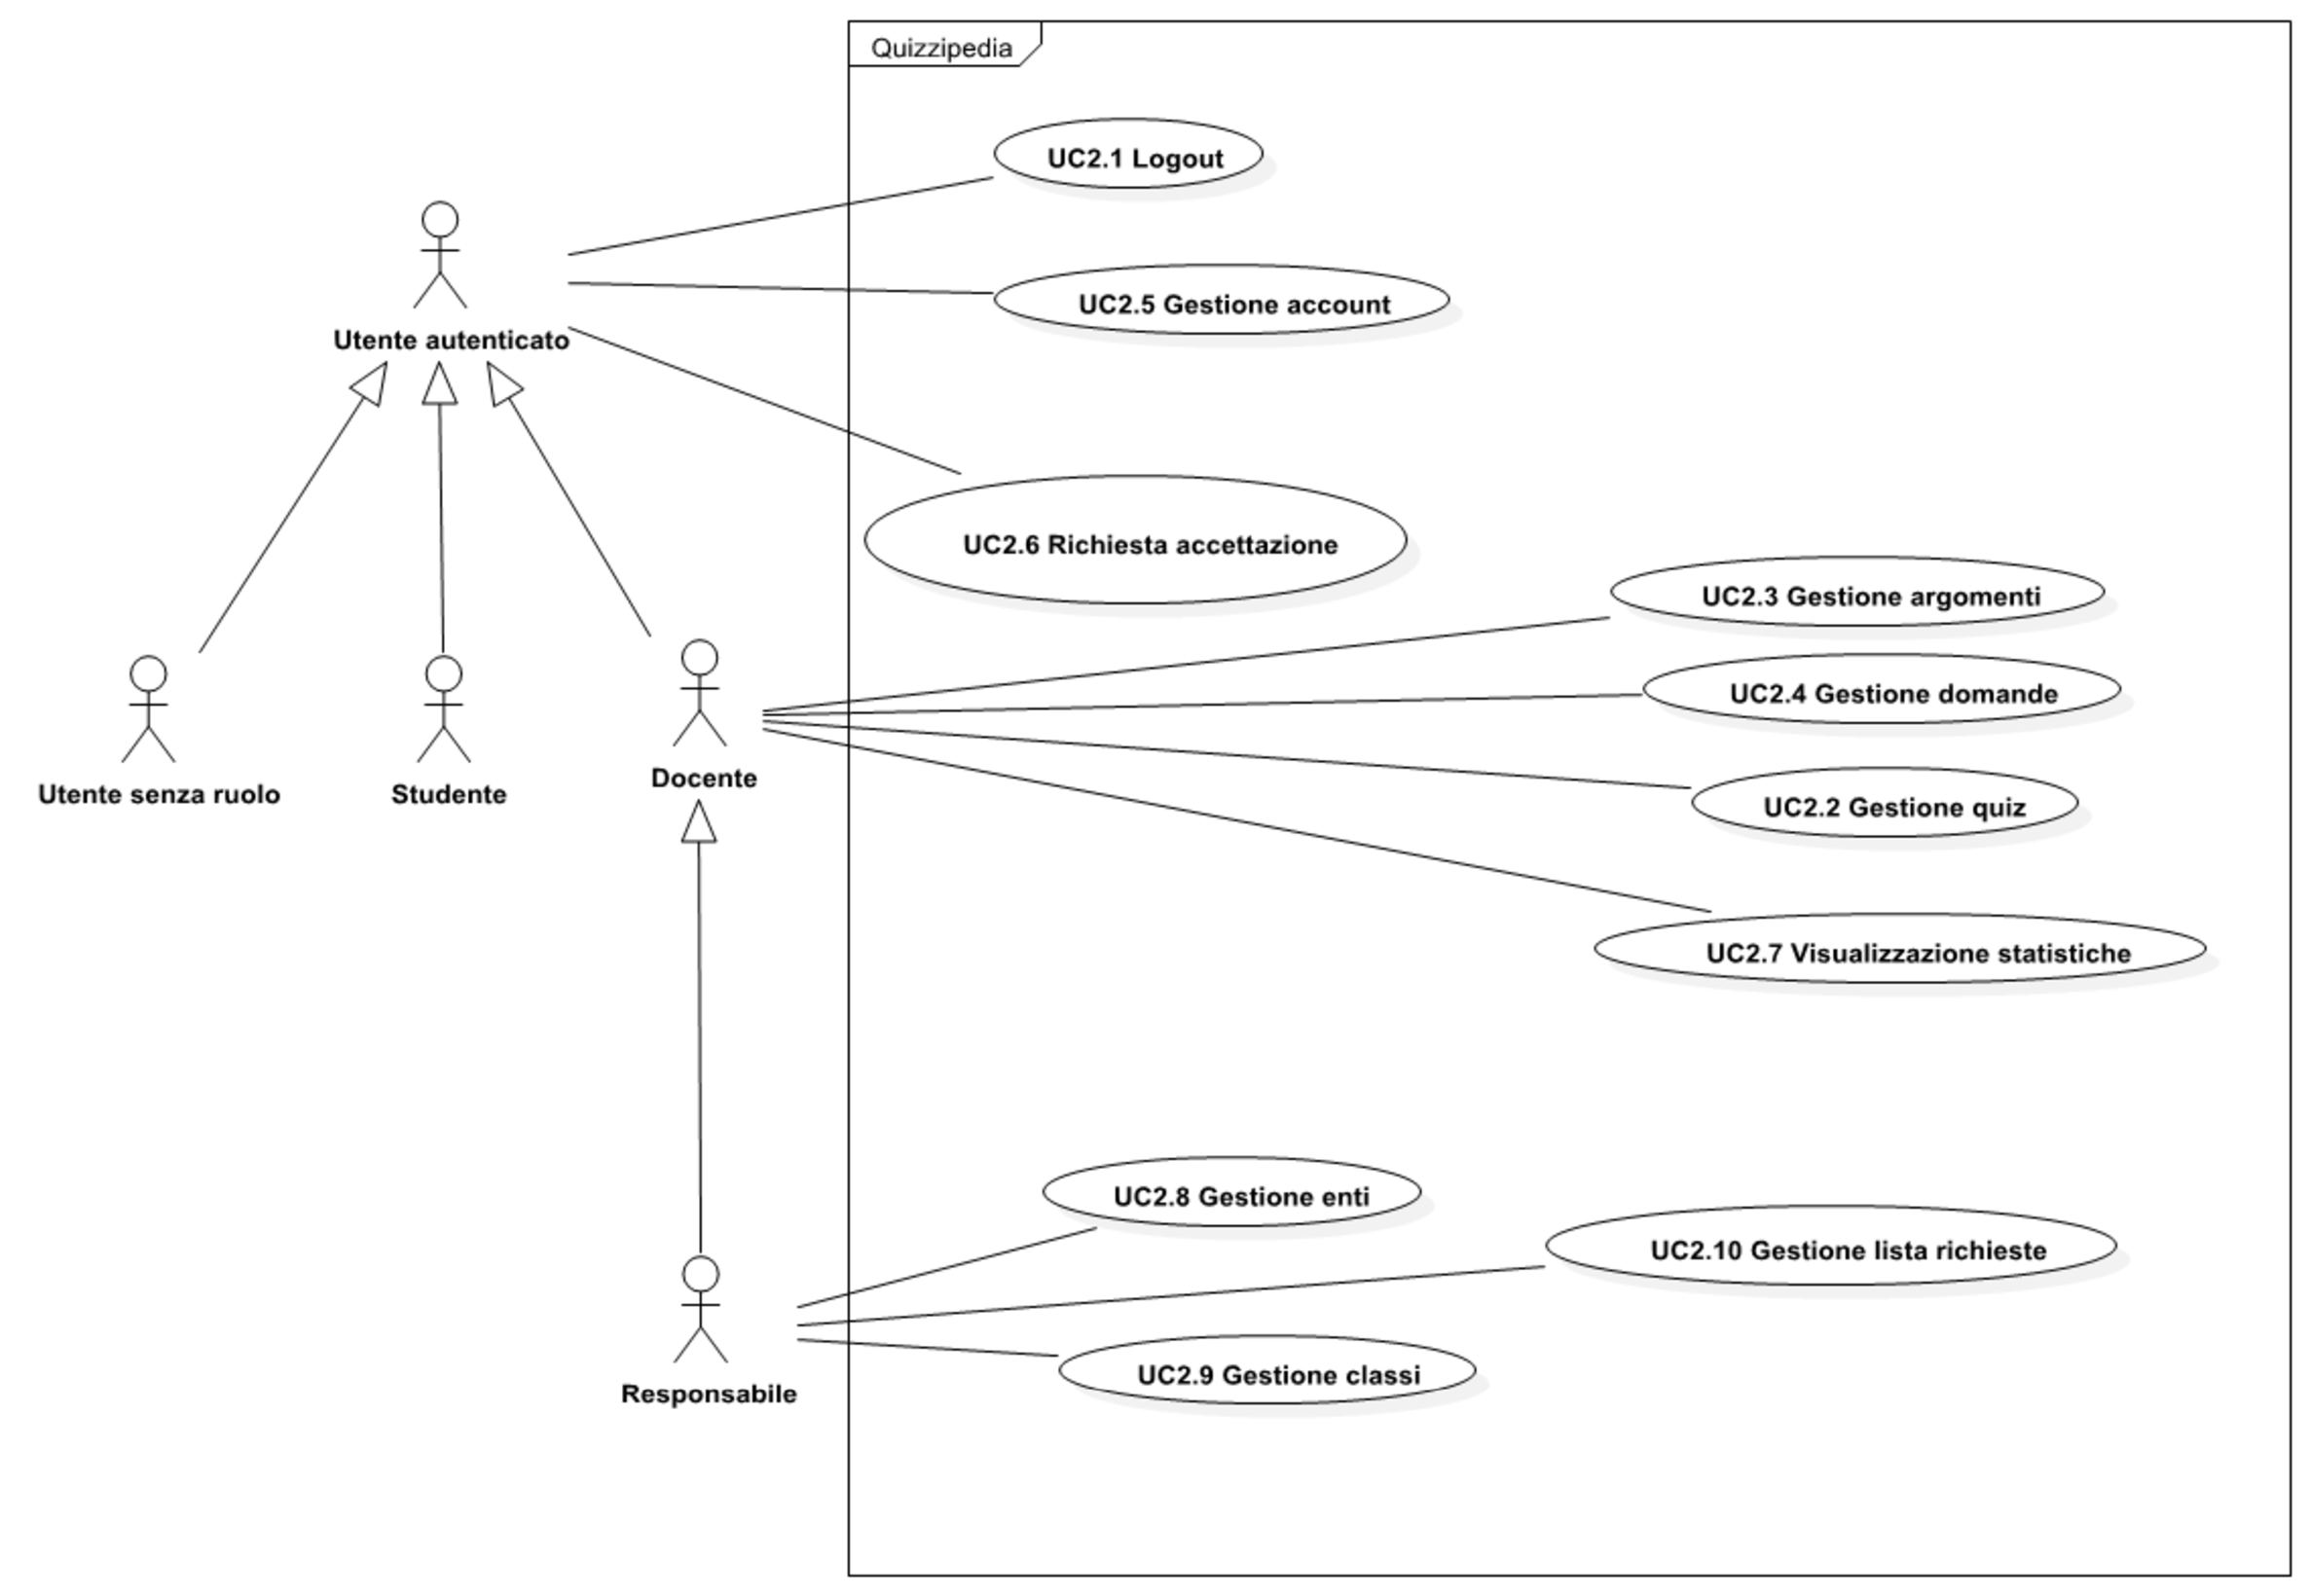
\includegraphics[width=\textwidth]{Img/UC Caso d'uso privato.pdf}}
\caption{UC2 Caso d'uso privato}
\end{figure}
\begin{itemize}
\item \textbf{Attori}: Utente Autenticato.
\item \textbf{Scenario principale}:
\begin{enumerate}
\item Logout (UC2.1);
\item Gestione quiz (UC2.2);
\item Gestione argomenti (UC2.3);
\item Gestione domande (UC2.4);
\item Gestione account (UC2.5);
\item Richiesta accettazione (UC2.6);
\item Visualizzazione statistiche (UC2.7);
\item Gestione enti (UC2.8);
\item Gestione classe (UC2.9);
\item Lista richieste (UC2.10);
\item Gestione domande (UC2.11).
\end{enumerate}
\item \textbf{Descrizione}: l'utente autenticato può accedere ad aree private a seconda dei permessi di cui dispone.
\item \textbf{Precondizione}: l'utente è in possesso di un account Quizzipedia e si è precedentemente autenticato.
\item \textbf{Postcondizione}: l'utente ha scelto l'operazione da intraprendere.
\end{itemize}
\subsubsection{UC2.1 Logout}
\begin{itemize}
\item \textbf{Attori}: Utente Autenticato.
\item \textbf{Descrizione}: l’utente può effettuare il logout dall’area privata.
\item \textbf{Precondizione}: l’utente è in possesso di un account Quizzipedia e si è precedentemente autenticato.
\item \textbf{Postcondizione}: l’utente ha effettuato il logout e ora non è più autenticato.
\end{itemize}
\subsubsection{UC2.2 Gestione quiz}
\begin{figure}[H]
\centering
\noindent\makebox[\textwidth]{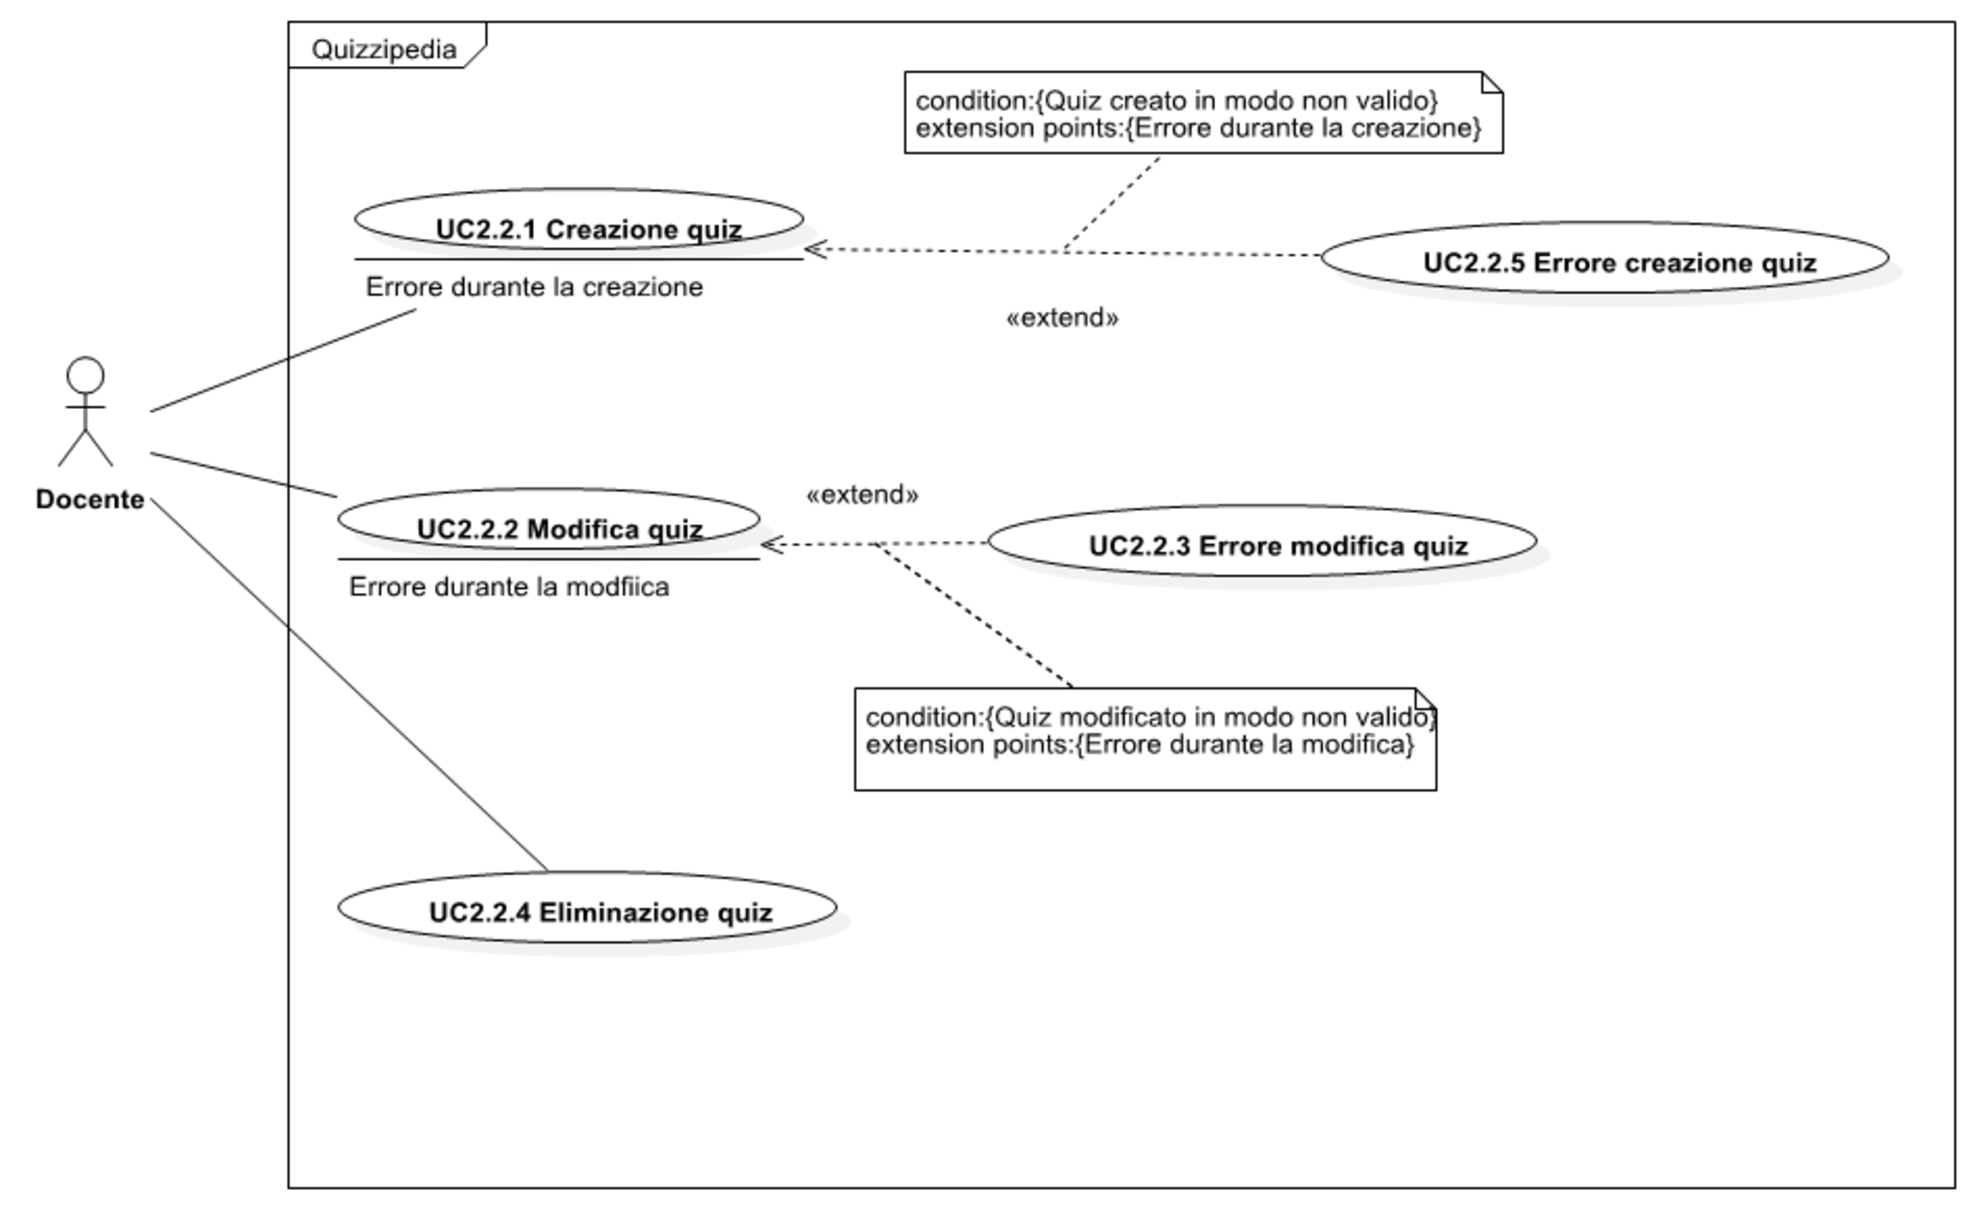
\includegraphics[width=\textwidth]{Img/UC Gestione quiz.pdf}}
\caption{UC2.2 Gestione quiz}
\end{figure}
\begin{itemize}
\item \textbf{Attori}: Docente.
\item \textbf{Scenario principale}:
\begin{enumerate}
\item Creazione quiz (UC2.2.1);
\item Modifica quiz (UC2.2.2);
\item Errore durante la modifica del quiz (UC2.2.3);
\item Eliminazione quiz (UC2.2.4);
\item Interruzione volontaria della creazione del quiz (UC2.2.5);
\item Interruzione volontaria della modifica del quiz (UC2.2.6).
\end{enumerate}
\item \textbf{Descrizione}: il docente deve poter effettuare varie operazioni di gestione di quiz, in particolare deve poter creare quiz nuovi e modificare o eliminare quiz esistenti.
\item \textbf{Precondizione}: il docente è autenticato nel sistema e desidera effettuare operazioni sui quiz.
\item \textbf{Postcondizione}: il docente ha effettuato le operazioni desiderate sui quiz.
\end{itemize}
\subsubsection{UC2.2.1 Creazione quiz}
\begin{figure}[H]
\centering
\noindent\makebox[\textwidth]{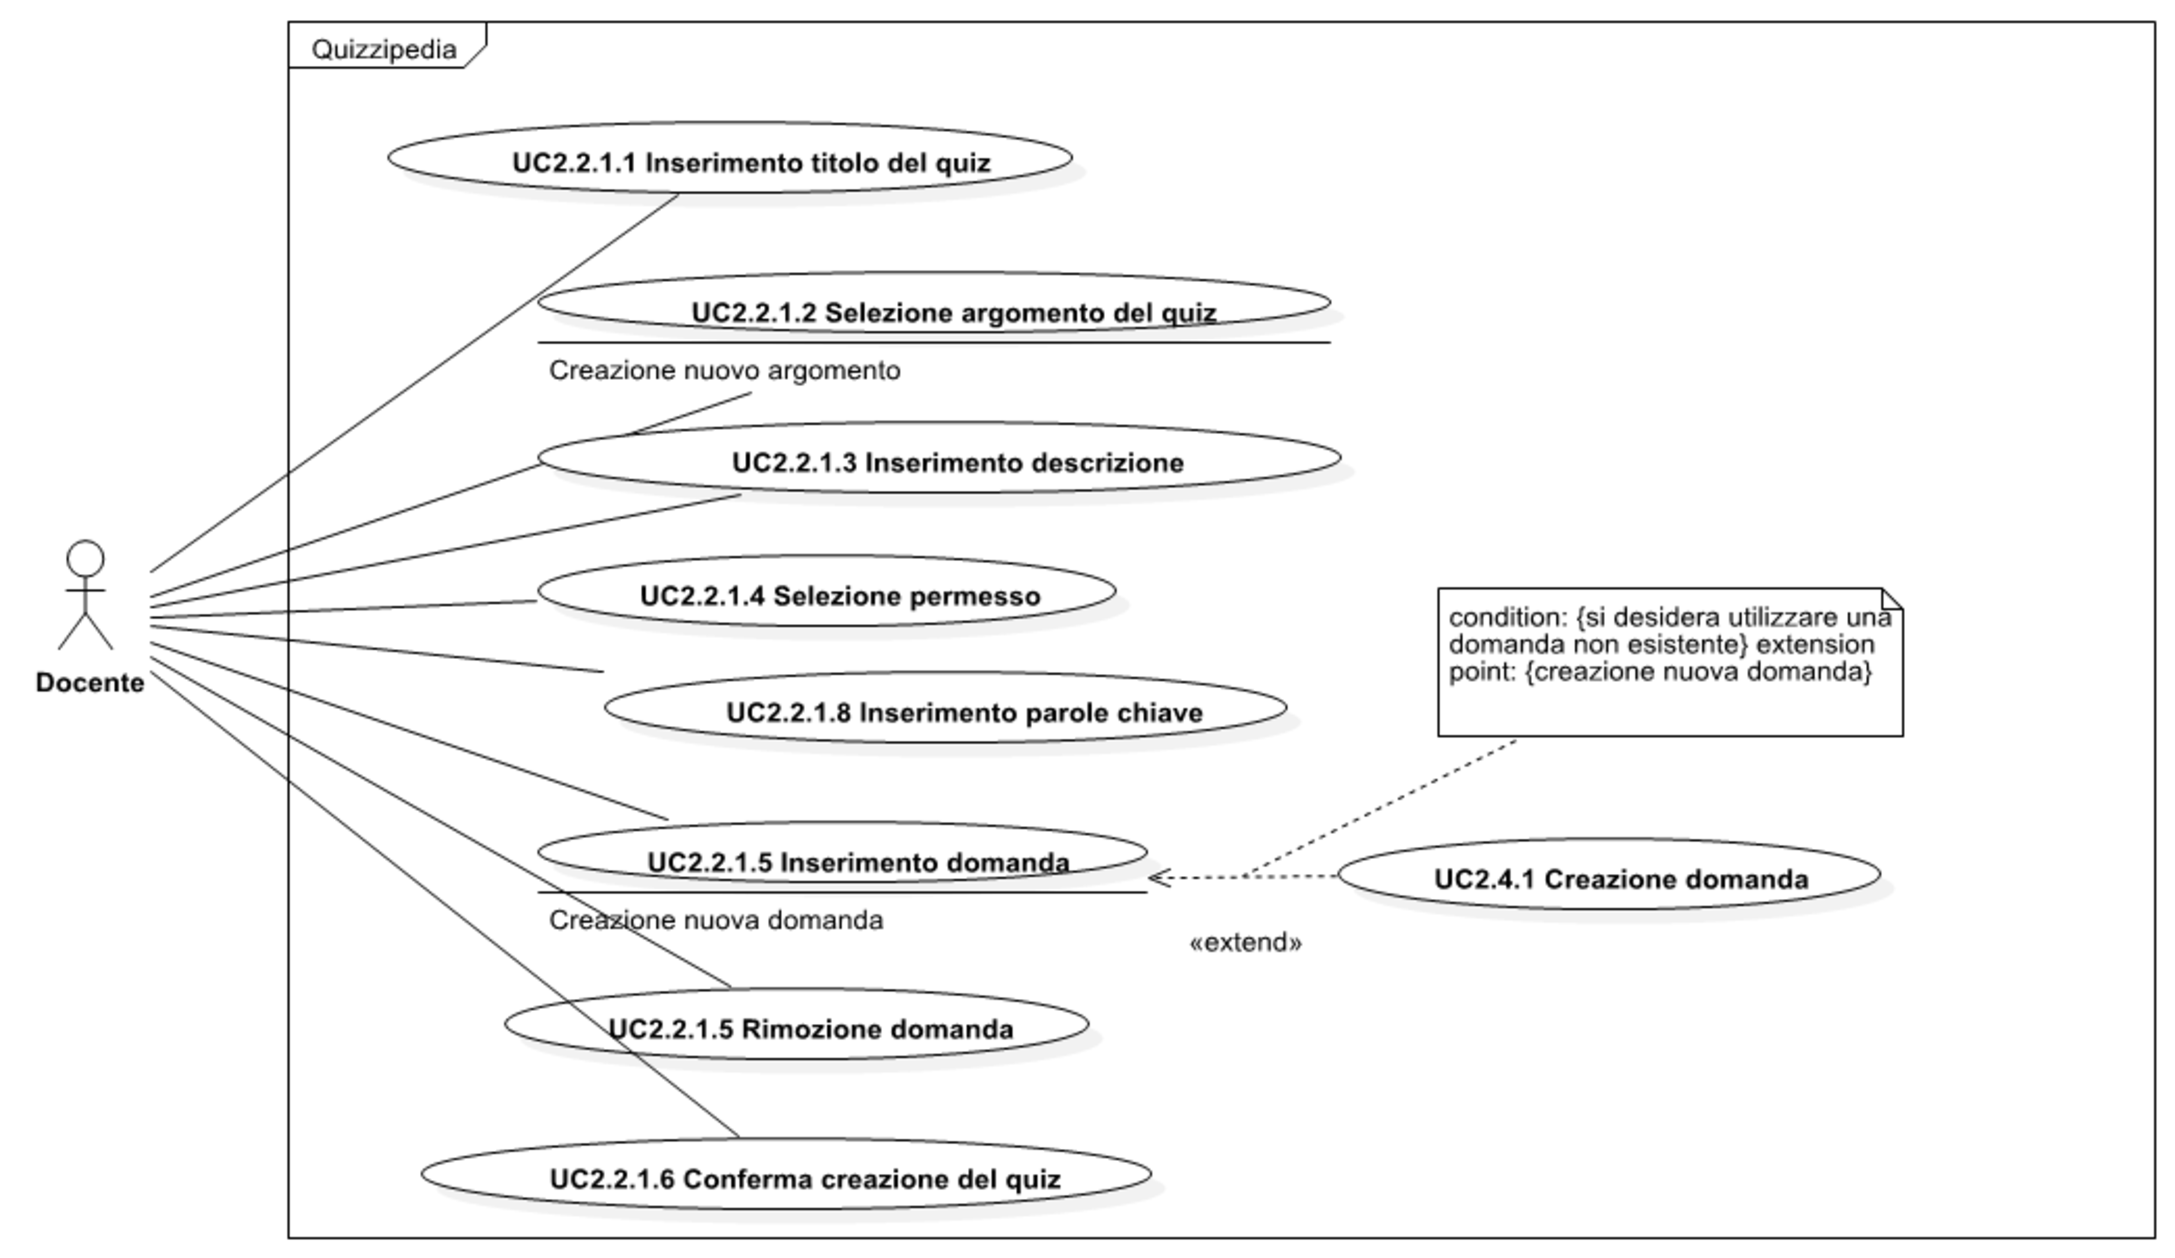
\includegraphics[width=\textwidth]{Img/UC Creazione quiz.pdf}}
\caption{UC2.2.1 Creazione quiz}
\end{figure}
\begin{itemize}
\item \textbf{Attori}: Docente.
\item \textbf{Scenario principale}:
\begin{enumerate}
\item Inserimento titolo (UC2.2.1.1);
\item Selezione argomento del quiz (UC2.2.1.2);
\item Inserimento descrizione (UC2.2.1.3);
\item Conferma creazione quiz (UC2.2.1.4).
\end{enumerate}
\item \textbf{Inclusioni}:
\begin{itemize}
\item Modifica quiz (UC2.2.2).
\end{itemize}
\item \textbf{Estensioni}:
\begin{itemize}
\item Interruzione volontaria della creazione del quiz (UC2.2.5).
\end{itemize}
\item \textbf{Descrizione}: il docente deve poter creare un nuovo quiz.
\item \textbf{Precondizione}: il docente è autenticato nel sistema e desidera creare un nuovo quiz.
\item \textbf{Postcondizione}: il docente ha creato il nuovo quiz.
\end{itemize}
\subsubsection{UC2.2.1.1 Inserimento titolo}
\begin{itemize}
\item \textbf{Attori}: Docente.
\item \textbf{Scenario principale}: il docente inserisce il titolo del quiz.
\item \textbf{Descrizione}: il docente deve poter inserire il titolo del quiz che sta creando.
\item \textbf{Precondizione}: il docente sta creando un nuovo quiz e deve ancora inserire il titolo.
\item \textbf{Postcondizione}: il docente ha inserito il titolo del quiz.
\end{itemize}
\subsubsection{UC2.2.1.2 Selezione argomento del quiz}
\begin{itemize}
\item \textbf{Attori}: Docente.
\item \textbf{Scenario principale}: il docente deleziona l'argomento del quiz.
\item \textbf{Estensioni}:
\begin{itemize}
\item Creazione argomento (UC2.3.1).
\end{itemize}
\item \textbf{Descrizione}: il docente deve poter selezionare l'argomento del quiz da una lista di argomenti, o creare un nuovo argomento se è mancante.
\item \textbf{Precondizione}: il docente sta creando un nuovo quiz e deve selezionare l'argomento.
\item \textbf{Postcondizione}: il docente ha selezionato l'argomento del quiz.
\end{itemize}
\subsubsection{UC2.2.1.3 Inserimento descrizione}
\begin{itemize}
\item \textbf{Attori}: Docente.
\item \textbf{Scenario principale}: il docente inserisce la descrizione del quiz.
\item \textbf{Descrizione}: il docente deve poter inserire la descrizione del quiz che sta creando.
\item \textbf{Precondizione}: il docente sta creando un nuovo quiz e deve ancora inserire la descrizione.
\item \textbf{Postcondizione}: il docente ha inserito la descrizione del quiz.
\end{itemize}
\subsubsection{UC2.2.1.4 Conferma creazione quiz}
\begin{itemize}
\item \textbf{Attori}: Docente.
\item \textbf{Scenario principale}: il docente conferma la creazione del quiz.
\item \textbf{Descrizione}: il docente deve confermare la creazione del nuovo quiz per portarla a termine.
\item \textbf{Precondizione}: il docente sta creando un nuovo quiz e deve ancora confermare la sua creazione.
\item \textbf{Postcondizione}: il docente ha confermato la creazione del quiz.
\end{itemize}
\subsubsection{UC2.2.2 Modifica quiz}
\begin{figure}[H]
\centering
\noindent\makebox[\textwidth]{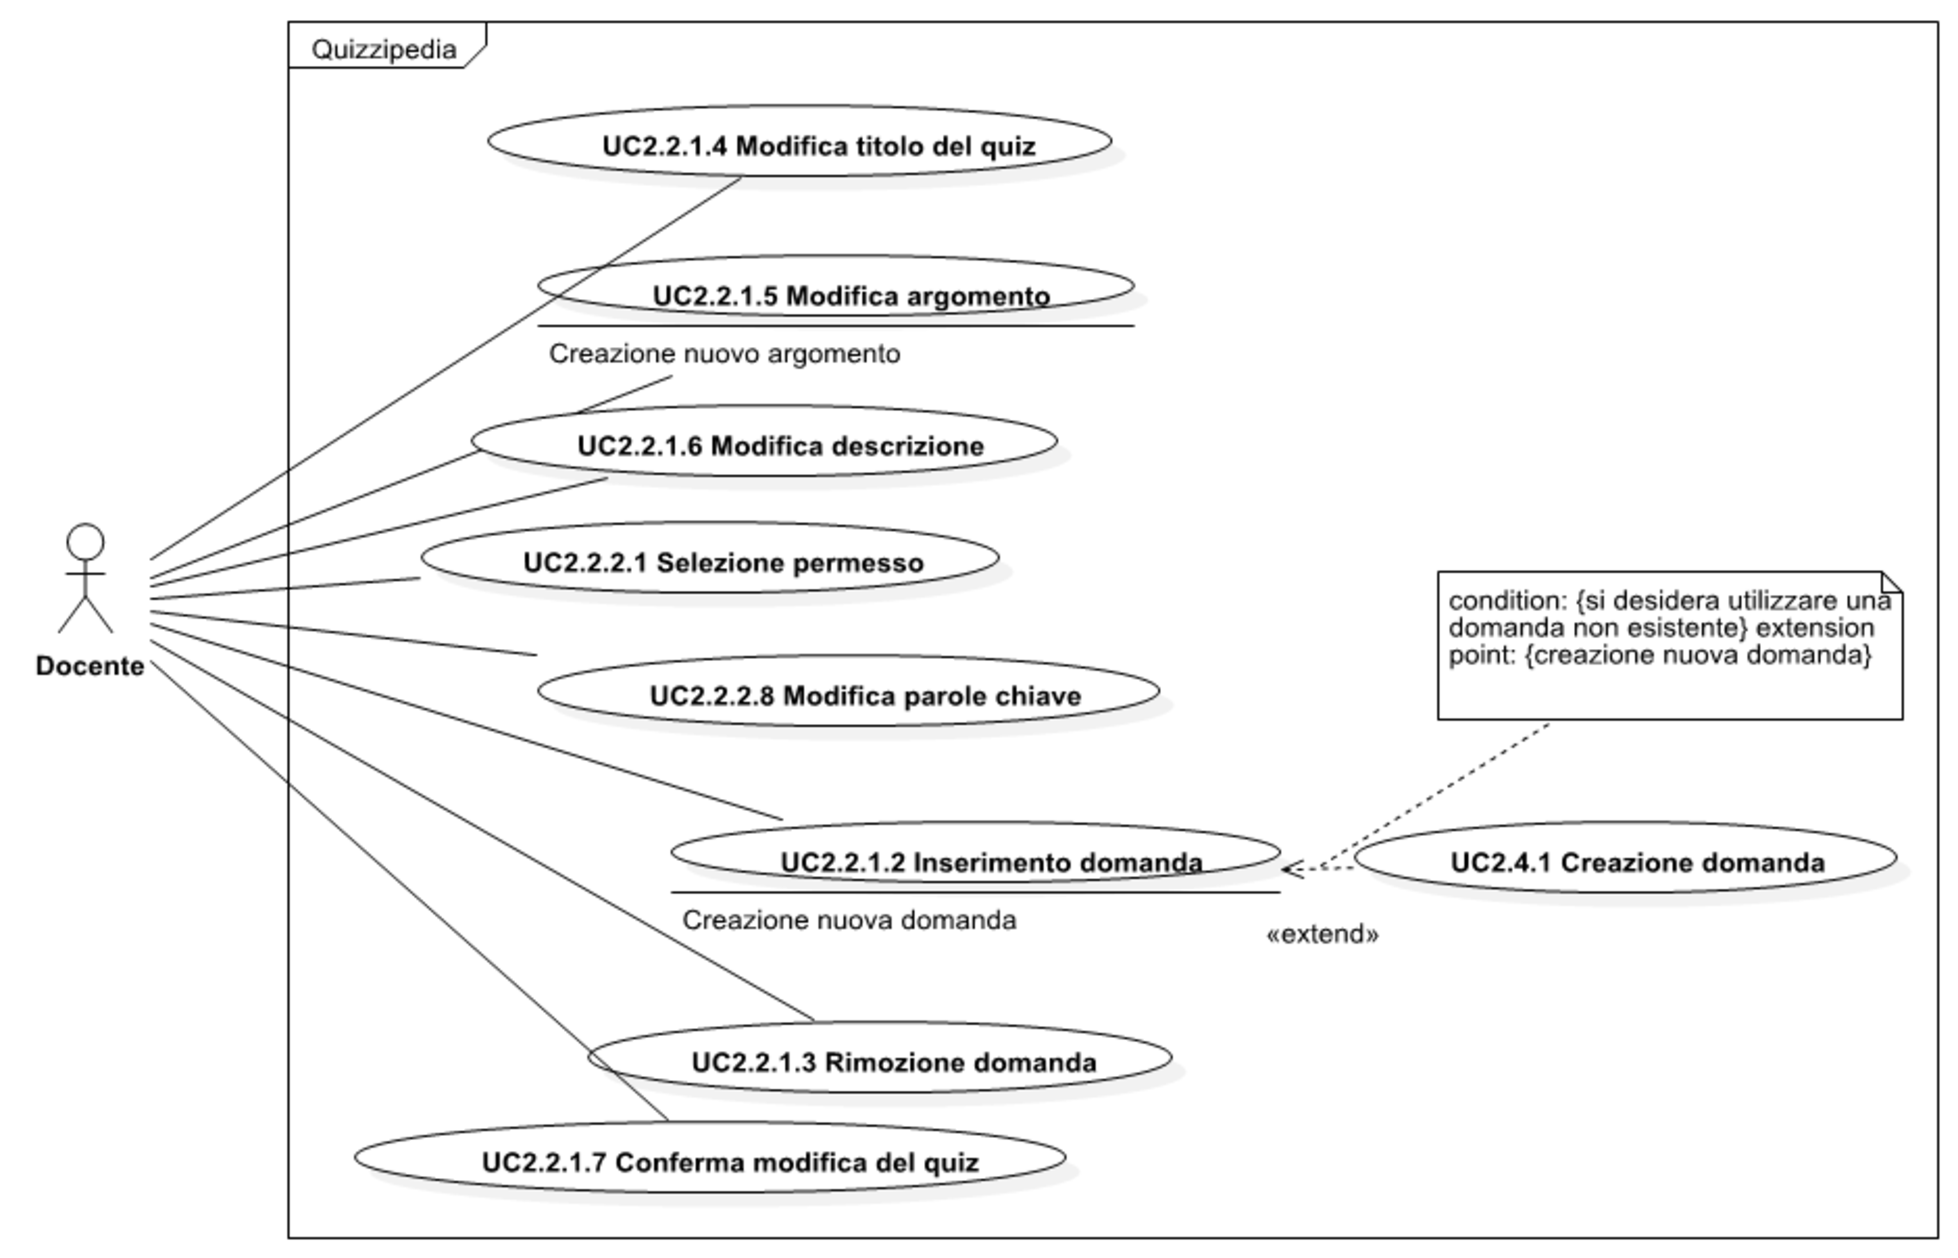
\includegraphics[width=\textwidth]{Img/UC Modifica quiz.pdf}}
\caption{UC2.2.2 Modifica quiz}
\end{figure}
\begin{itemize}
\item \textbf{Attori}: Docente.
\item \textbf{Scenario principale}:
\begin{enumerate}
\item Selezione permesso (UC2.2.2.1);
\item Inserimento domanda nel quiz (UC2.2.2.2);
\item Rimozione domanda dal quiz (UC2.2.2.3);
\item Modifica titolo (UC2.2.2.4);
\item Modifica argomento (UC2.2.2.5);
\item Modifica descrizione (UC2.2.2.6);
\item Conferma modifica quiz (UC2.2.2.7).
\end{enumerate}
\item \textbf{Estensioni}:
\begin{itemize}
\item Errore durante la modifica del quiz (UC2.2.3);
\item Interruzione volontaria della modifica del quiz (UC2.2.6).
\end{itemize}
\item \textbf{Descrizione}: il docente deve poter modificare un quiz.
\item \textbf{Precondizione}: il docente è autenticato nel sistema e desidera modificare un quiz.
\item \textbf{Postcondizione}: il docente ha modificato il quiz.
\end{itemize}
\subsubsection{UC2.2.2.1 Selezione permesso}
\begin{figure}[H]
\centering
\noindent\makebox[\textwidth]{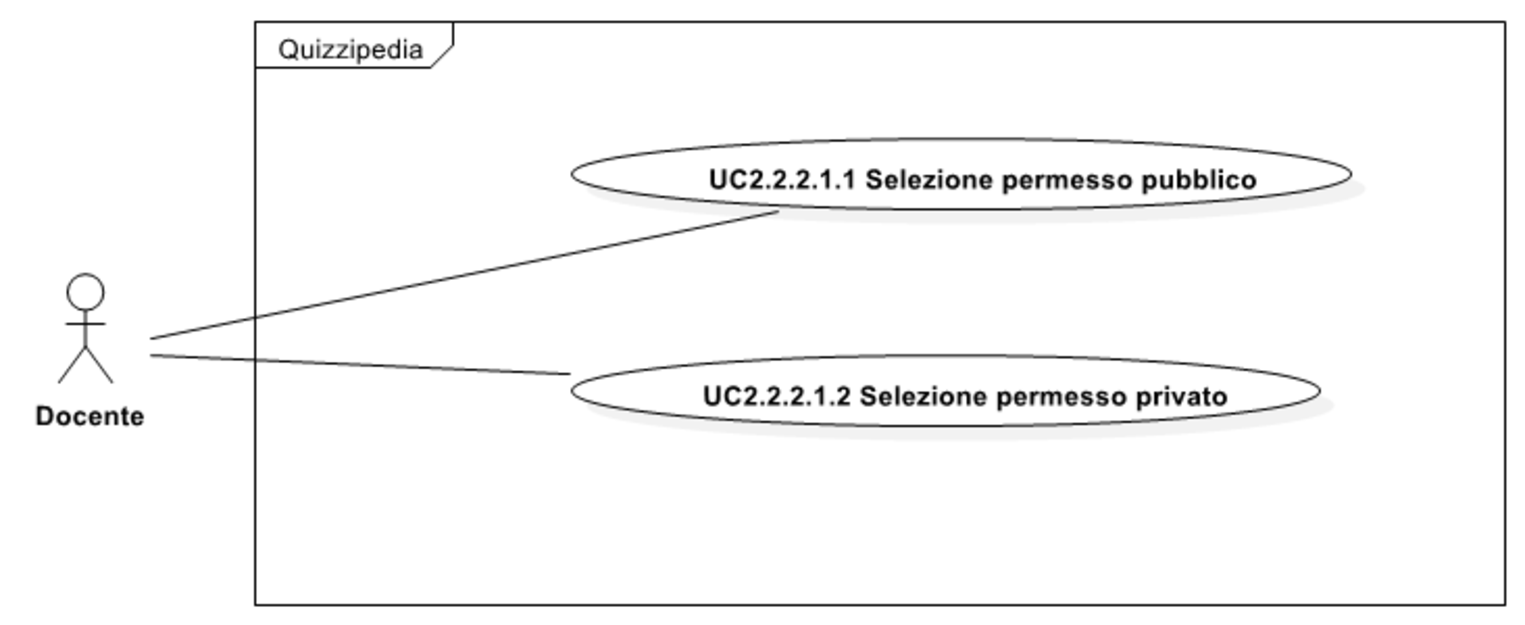
\includegraphics[width=\textwidth]{Img/UC Selezione permesso.pdf}}
\caption{UC2.2.2.1 Selezione permesso}
\end{figure}
\begin{itemize}
\item \textbf{Attori}: Docente.
\item \textbf{Scenario principale}:
\begin{enumerate}
\item Selezione permesso pubblico (UC2.2.2.1.1);
\item Selezione permesso privato (UC2.2.2.1.2).
\end{enumerate}
\item \textbf{Descrizione}: il docente deve poter scegliere il permesso del quiz.
\item \textbf{Precondizione}: il docente sta modificando un quiz.
\item \textbf{Postcondizione}: il docente ha specificato il permesso del quiz.
\end{itemize}
\subsubsection{UC2.2.2.1.1 Selezione permesso pubblico}
\begin{itemize}
\item \textbf{Attori}: Responsabile.
\item \textbf{Scenario principale}: il docente seleziona il permesso 'pubblico' per il quiz.
\item \textbf{Descrizione}: il docente ha scelto un permesso 'pubblico' per il quiz, permettendo a tutti gli utenti di svolgerlo senza restrizioni.
\item \textbf{Precondizione}: il docente sta selezionando il permesso di un quiz.
\item \textbf{Postcondizione}: il docente ha scelto il permesso 'pubblico'.
\end{itemize}
\subsubsection{UC2.2.2.1.2 Selezione permesso privato}
\begin{figure}[H]
\centering
\noindent\makebox[\textwidth]{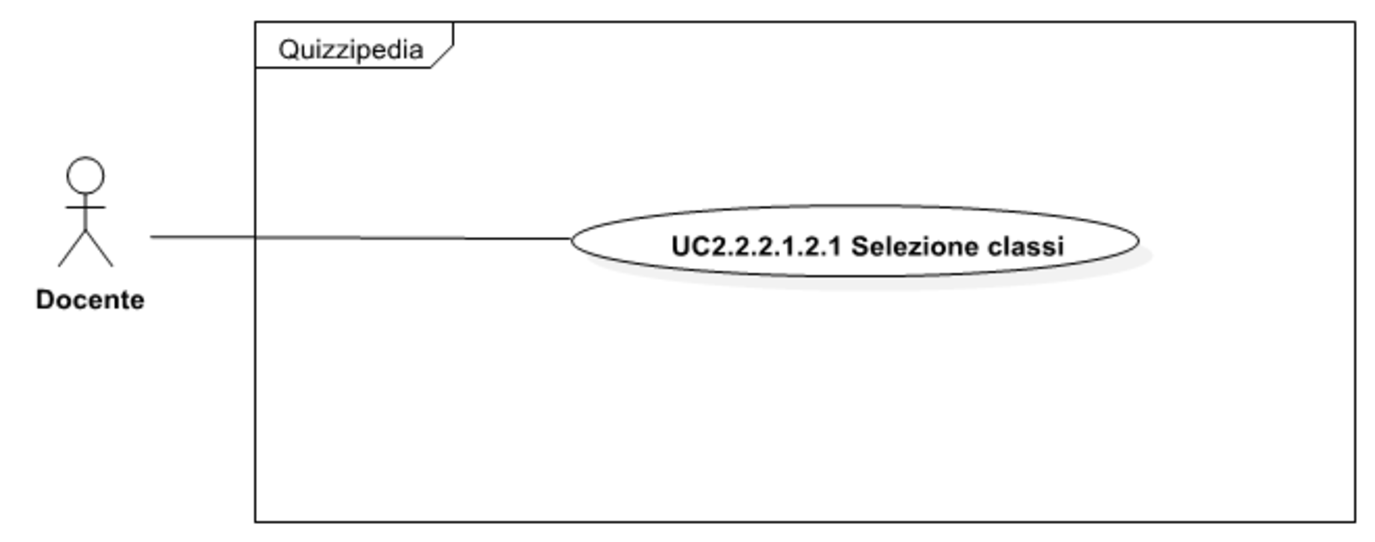
\includegraphics[width=\textwidth]{Img/UC Selezione permesso privato.pdf}}
\caption{UC2.2.2.1.2 Selezione permesso privato}
\end{figure}
\begin{itemize}
\item \textbf{Attori}: Docente.
\item \textbf{Scenario principale}:
\begin{enumerate}
\item Selezione classi (UC2.2.2.1.2.1).
\end{enumerate}
\item \textbf{Descrizione}: il docente ha scelto un permesso privato per il quiz, limitando il suo accesso e svolgimento a una cerchia ristretta di studenti.
\item \textbf{Precondizione}: il docente sta selezionando il permesso di un quiz.
\item \textbf{Postcondizione}: il docente ha scelto il permesso privato.
\end{itemize}
\subsubsection{UC2.2.2.1.2.1 Selezione classi}
\begin{itemize}
\item \textbf{Attori}: Docente.
\item \textbf{Scenario principale}: il docente seleziona le classi a cui assegnare il quiz privato.
\item \textbf{Descrizione}: il docente può assegnare il quiz privato a una o più classi di studenti, i cui partecipanti avranno diritto di svolgerlo.
\item \textbf{Precondizione}: il docente ha selezionato un permesso 'privato' per il quiz.
\item \textbf{Postcondizione}: il docente ha selezionato le classi a cui assegnare il quiz.
\end{itemize}
\subsubsection{UC2.2.2.2 Inserimento domanda nel quiz}
\begin{itemize}
\item \textbf{Attori}: Docente.
\item \textbf{Scenario principale}: il docente inserisce una domanda nel quiz.
\item \textbf{Descrizione}: il docente deve poter inserire una domanda nel quiz.
\item \textbf{Precondizione}: il docente sta modificando un quiz e vuole inserire una domanda.
\item \textbf{Postcondizione}: il docente ha inserito la domanda.
\end{itemize}
\subsubsection{UC2.2.2.3 Rimozione domanda dal quiz}
\begin{itemize}
\item \textbf{Attori}: Docente.
\item \textbf{Scenario principale}: il docente rimuove una domanda dal quiz.
\item \textbf{Descrizione}: il docente deve poter rimuovere una domanda nel quiz (la domanda non sarà cancellata ma soltanto rimossa dal quiz).
\item \textbf{Precondizione}: il docente sta modificando il quiz e vuole rimuovere una domanda.
\item \textbf{Postcondizione}: il docente ha rimosso la domanda.
\end{itemize}
\subsubsection{UC2.2.2.4 Modifica titolo}
\begin{itemize}
\item \textbf{Attori}: Docente.
\item \textbf{Scenario principale}: il docente modifica il titolo del quiz.
\item \textbf{Descrizione}: il docente deve poter modificare il titolo del quiz.
\item \textbf{Precondizione}: il docente sta modificando un nuovo quiz.
\item \textbf{Postcondizione}: il docente ha modificato il titolo del quiz.
\end{itemize}
\subsubsection{UC2.2.2.5 Modifica argomento}
\begin{figure}[H]
\centering
\noindent\makebox[\textwidth]{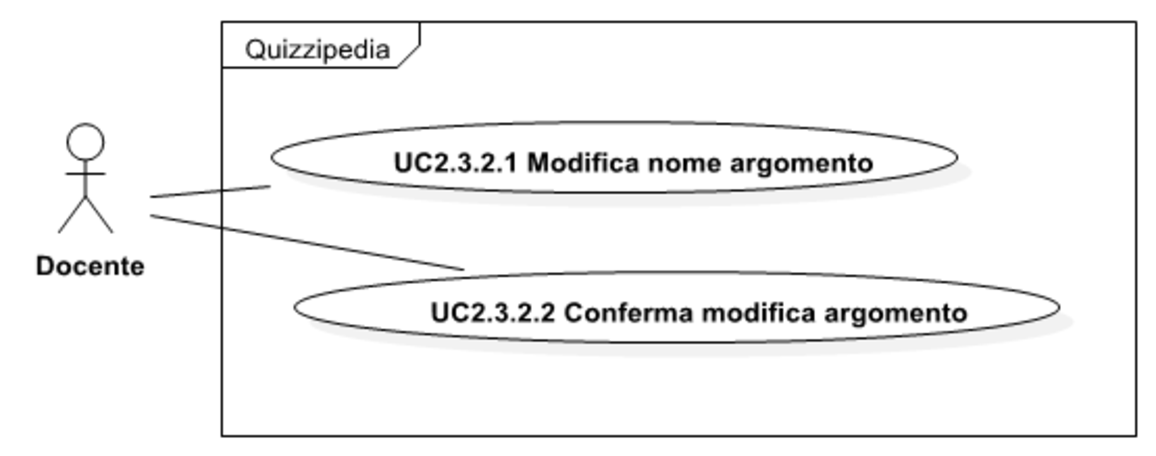
\includegraphics[width=\textwidth]{Img/UC Modifica argomento.pdf}}
\caption{UC2.2.2.5 Modifica argomento}
\end{figure}
\begin{itemize}
\item \textbf{Attori}: Docente.
\item \textbf{Scenario principale}: il docente modifica l'argomento del quiz.
\item \textbf{Estensioni}:
\begin{itemize}
\item Creazione argomento (UC2.3.1).
\end{itemize}
\item \textbf{Descrizione}: il docente deve poter selezionare l'argomento del quiz da una lista di argomenti, o creare un nuovo argomento se è mancante.
\item \textbf{Precondizione}: il docente sta modificando un quiz.
\item \textbf{Postcondizione}: il docente ha modificato l'argomento del quiz.
\end{itemize}
\subsubsection{UC2.2.2.6 Modifica descrizione}
\begin{itemize}
\item \textbf{Attori}: Docente.
\item \textbf{Scenario principale}: il docente modifica la descrizione del quiz.
\item \textbf{Descrizione}: il docente deve poter modificare la descrizione del quiz.
\item \textbf{Precondizione}: il docente sta modificando un quiz.
\item \textbf{Postcondizione}: il docente ha modificato la descrizione del quiz.
\end{itemize}
\subsubsection{UC2.2.2.7 Conferma modifica quiz}
\begin{itemize}
\item \textbf{Attori}: Docente.
\item \textbf{Scenario principale}: il docente conferma la modifica del quiz.
\item \textbf{Descrizione}: il docente deve confermare la modifica del quiz per portarla a termine.
\item \textbf{Precondizione}: il docente sta modificando un quiz e deve ancora confermare la sua modifica.
\item \textbf{Postcondizione}: il docente ha confermato la modifica del quiz.
\end{itemize}
\subsubsection{UC2.2.3 Errore durante la modifica del quiz}
\begin{itemize}
\item \textbf{Attori}: Docente.
\item \textbf{Scenario principale}: il docente visualizza il messaggio di errore.
\item \textbf{Descrizione}: si è verificata la seguente condizione: il numero di risposte selezionate è eccessivo o pari a zero.
\item \textbf{Precondizione}: il docente ha iniziato una modifica del quiz che non è andata a buon termine.
\item \textbf{Postcondizione}: il docente ha visualizzato l'errore.
\end{itemize}
\subsubsection{UC2.2.4 Eliminazione quiz}
\begin{figure}[H]
\centering
\noindent\makebox[\textwidth]{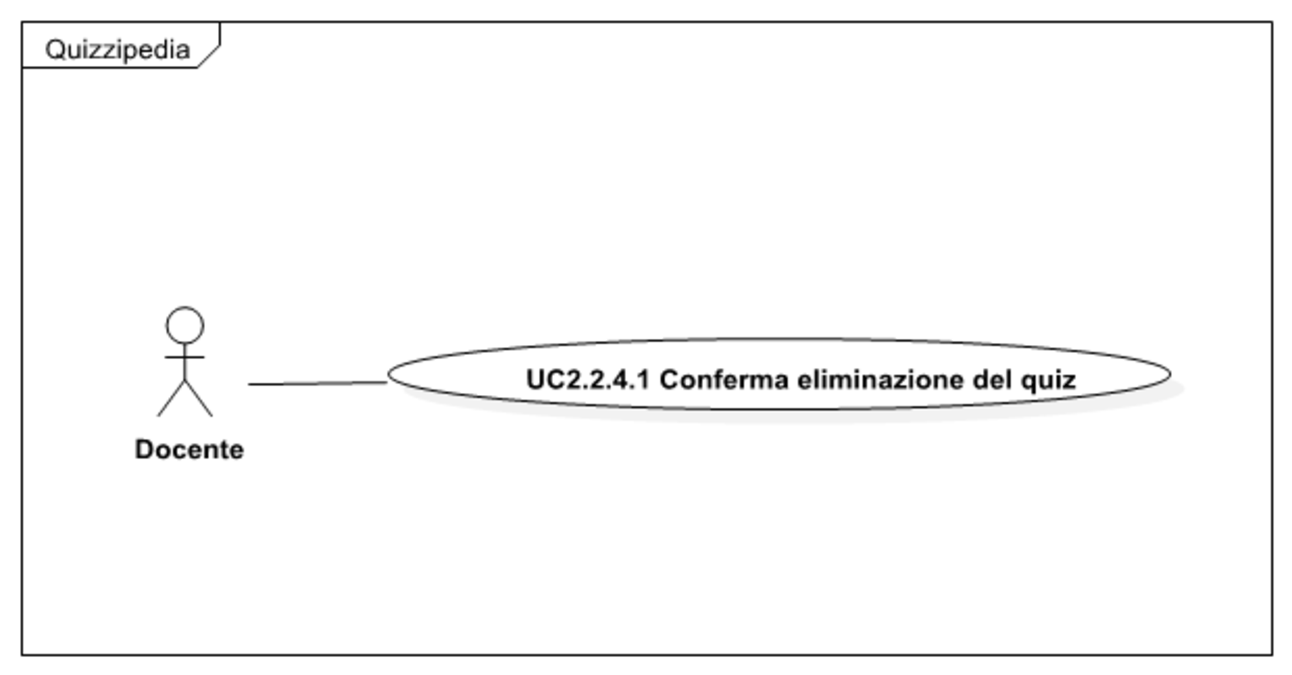
\includegraphics[width=\textwidth]{Img/UC Eliminazione quiz.pdf}}
\caption{UC2.2.4 Eliminazione quiz}
\end{figure}
\begin{itemize}
\item \textbf{Attori}: Docente.
\item \textbf{Scenario principale}:
\begin{enumerate}
\item conferma eliminazione del quiz (UC2.2.4.1);
\item Interruzione volontaria della modifica della domanda (UC2.2.4.2).
\end{enumerate}
\item \textbf{Descrizione}: il docente deve poter eliminare un quiz. Questo non causerà l’eliminazione delle domande contenute nel quiz.
\item \textbf{Precondizione}: il docente è autenticato nel sistema e desidera eliminare un quiz esistente.
\item \textbf{Postcondizione}: il docente ha eliminato il quiz.
\end{itemize}
\subsubsection{UC2.2.4.1 conferma eliminazione del quiz}
\begin{itemize}
\item \textbf{Attori}: Docente.
\item \textbf{Scenario principale}: il docente conferma l'eliminazione del quiz.
\item \textbf{Descrizione}: il docente dovrà confermare l'eliminazione del quiz.
\item \textbf{Precondizione}: il docente ha richiesto l'eliminazione di un quiz e deve ancora effettuare la conferma.
\item \textbf{Postcondizione}: il docente ha confermato l'eliminazione del quiz.
\end{itemize}
\subsubsection{UC2.2.4.2 Interruzione volontaria della modifica della domanda}
\begin{itemize}
\item \textbf{Attori}: Docente.
\item \textbf{Scenario principale}: il docente interrompe la modifica della domanda.
\item \textbf{Descrizione}: Il docente interrompe la modifica della domanda.
\item \textbf{Precondizione}: Il docente sta modificando una domanda.
\item \textbf{Postcondizione}: Il docente non ha completato la modifica della domanda.
\end{itemize}
\subsubsection{UC2.2.5 Interruzione volontaria della creazione del quiz}
\begin{itemize}
\item \textbf{Attori}: Docente.
\item \textbf{Scenario principale}: il docente interrompe la creazione del quiz.
\item \textbf{Descrizione}: Il docente interrompe la creazione del quiz.
\item \textbf{Precondizione}: Il docente sta creando un quiz.
\item \textbf{Postcondizione}: Il docente non completa la creazione del quiz.
\end{itemize}
\subsubsection{UC2.2.6 Interruzione volontaria della modifica del quiz}
\begin{itemize}
\item \textbf{Attori}: Docente.
\item \textbf{Scenario principale}: il docente interrompe la modifica del quiz.
\item \textbf{Descrizione}: Il docente interrompe la modifica del quiz.
\item \textbf{Precondizione}: Il docente sta modificando un quiz.
\item \textbf{Postcondizione}: Il docente non ha completato la modifica del quiz.
\end{itemize}
\subsubsection{UC2.3 Gestione argomenti}
\begin{figure}[H]
\centering
\noindent\makebox[\textwidth]{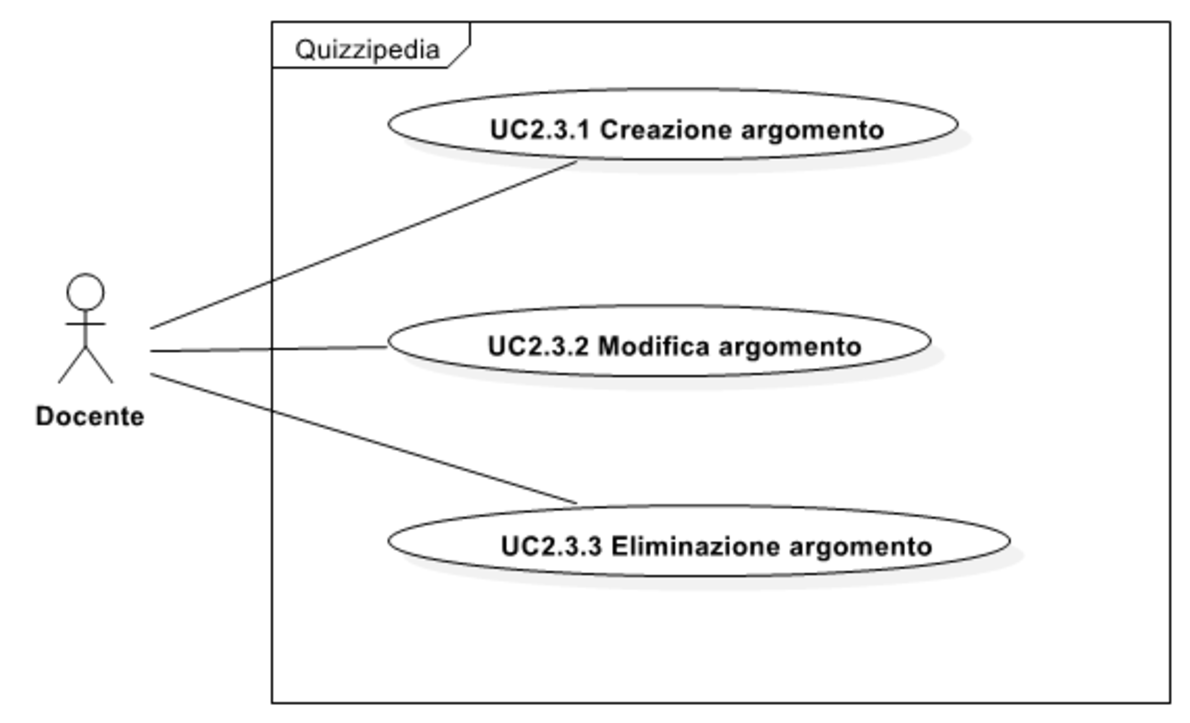
\includegraphics[width=\textwidth]{Img/UC Gestione argomenti.pdf}}
\caption{UC2.3 Gestione argomenti}
\end{figure}
\begin{itemize}
\item \textbf{Attori}: Docente.
\item \textbf{Scenario principale}:
\begin{enumerate}
\item Creazione argomento (UC2.3.1);
\item Modifica argomento (UC2.3.2);
\item Rimozione argomento (UC2.3.3).
\end{enumerate}
\item \textbf{Descrizione}: il docente deve poter gestire gli argomenti di quiz e domande, in particolare può inserire nuovi argomenti e modificare o eliminare argomenti esistenti.
\item \textbf{Precondizione}: il docente è autenticato e desidera effettuare operazioni sugli argomenti.
\item \textbf{Postcondizione}: il docente ha effettuato le operazioni sugli argomenti.
\end{itemize}
\subsubsection{UC2.3.1 Creazione argomento}
\begin{figure}[H]
\centering
\noindent\makebox[\textwidth]{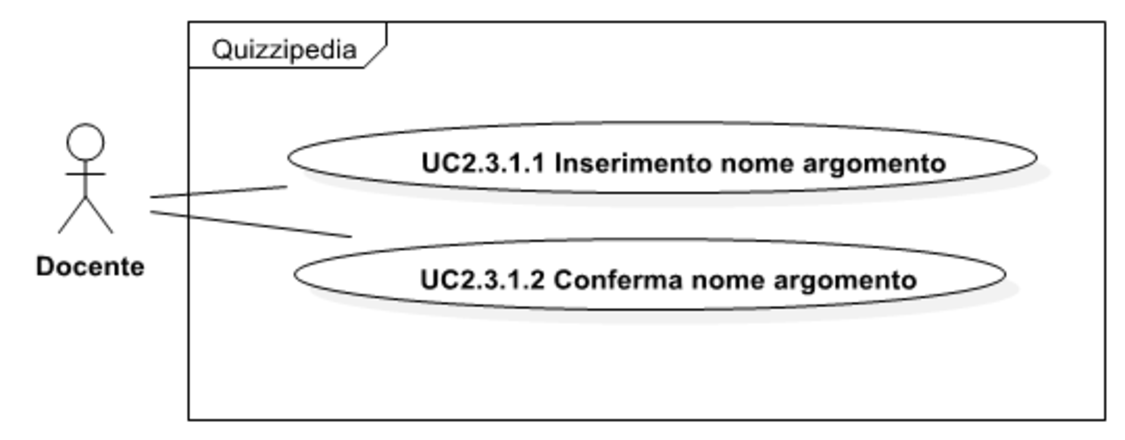
\includegraphics[width=\textwidth]{Img/UC Creazione argomento.pdf}}
\caption{UC2.3.1 Creazione argomento}
\end{figure}
\begin{itemize}
\item \textbf{Attori}: Docente.
\item \textbf{Scenario principale}:
\begin{enumerate}
\item Inserimento nome argomento (UC2.3.1.1);
\item Conferma creazione argomento (UC2.3.1.2).
\end{enumerate}
\item \textbf{Descrizione}: il docente deve poter creare un nuovo argomento.
\item \textbf{Precondizione}: il docente è autenticato e vuole creare un nuovo argomento.
\item \textbf{Postcondizione}: il docente ha creato il nuovo argomento.
\end{itemize}
\subsubsection{UC2.3.1.1 Inserimento nome argomento}
\begin{itemize}
\item \textbf{Attori}: Docente.
\item \textbf{Scenario principale}: il docente inserisce il nome dell'argomento.
\item \textbf{Descrizione}: il docente deve poter inserire il nome dell'argomento.
\item \textbf{Precondizione}: il docente sta creando un nuovo argomento e deve ancora inserire il nome.
\item \textbf{Postcondizione}: il docente ha inserito il nome dell'argomento.
\end{itemize}
\subsubsection{UC2.3.1.2 Conferma creazione argomento}
\begin{itemize}
\item \textbf{Attori}: Docente.
\item \textbf{Scenario principale}: il docente conferma la creazione dell'argomento.
\item \textbf{Descrizione}: il docente deve poter confermare la creazione dell'argomento.
\item \textbf{Precondizione}: il docente ha inserito un nuovo argomento e deve ancora confermare.
\item \textbf{Postcondizione}: il docente ha confermato il nuovo argomento.
\end{itemize}
\subsubsection{UC2.3.2 Modifica argomento}
\begin{figure}[H]
\centering
\noindent\makebox[\textwidth]{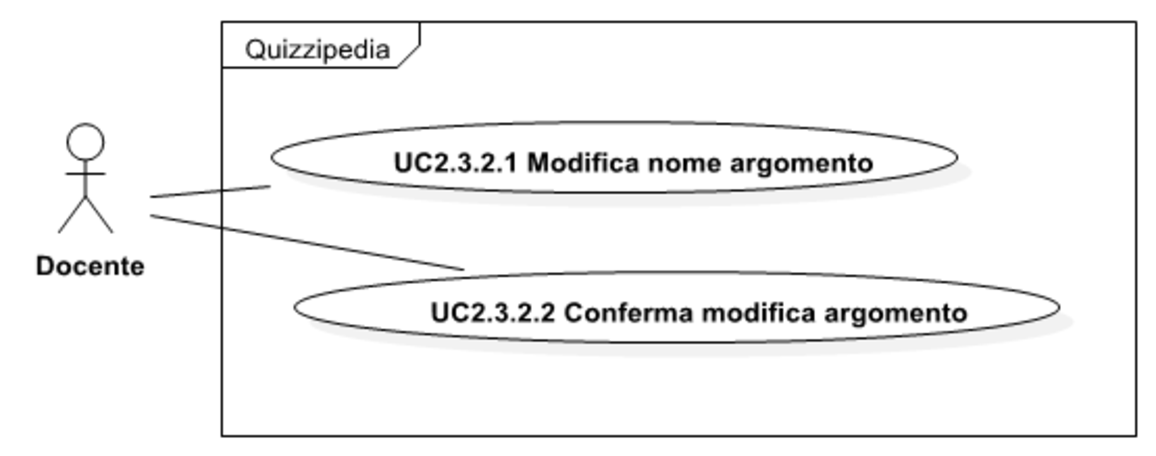
\includegraphics[width=\textwidth]{Img/UC Modifica argomento.pdf}}
\caption{UC2.3.2 Modifica argomento}
\end{figure}
\begin{itemize}
\item \textbf{Attori}: Docente.
\item \textbf{Scenario principale}:
\begin{enumerate}
\item Modifica nome argomento (UC2.3.2.1);
\item Conferma modifica argomento (UC2.3.2.2).
\end{enumerate}
\item \textbf{Descrizione}: il docente deve poter modificare un argomento.
\item \textbf{Precondizione}: il docente vuole modificare un argomento.
\item \textbf{Postcondizione}: il docente ha modificato un argomento .
\end{itemize}
\subsubsection{UC2.3.2.1 Modifica nome argomento}
\begin{itemize}
\item \textbf{Attori}: Docente.
\item \textbf{Scenario principale}: il docente modifica il nome dell'argomento.
\item \textbf{Descrizione}: il docente deve poter modificare il nome dell'argomento.
\item \textbf{Precondizione}: il docente è autenticato e sta gestendo un argomento.
\item \textbf{Postcondizione}: il docente ha modificato il nome di un argomento.
\end{itemize}
\subsubsection{UC2.3.2.2 Conferma modifica argomento}
\begin{itemize}
\item \textbf{Attori}: Docente.
\item \textbf{Scenario principale}: il docente conferma la modifica dell'argomento.
\item \textbf{Descrizione}: il docente deve poter confermare la modifica dell'argomento.
\item \textbf{Precondizione}: il docente ha modificato un argomento e deve confermare la modifica.
\item \textbf{Postcondizione}: il docente ha confermato la modifica.
\end{itemize}
\subsubsection{UC2.3.3 Rimozione argomento}
\begin{figure}[H]
\centering
\noindent\makebox[\textwidth]{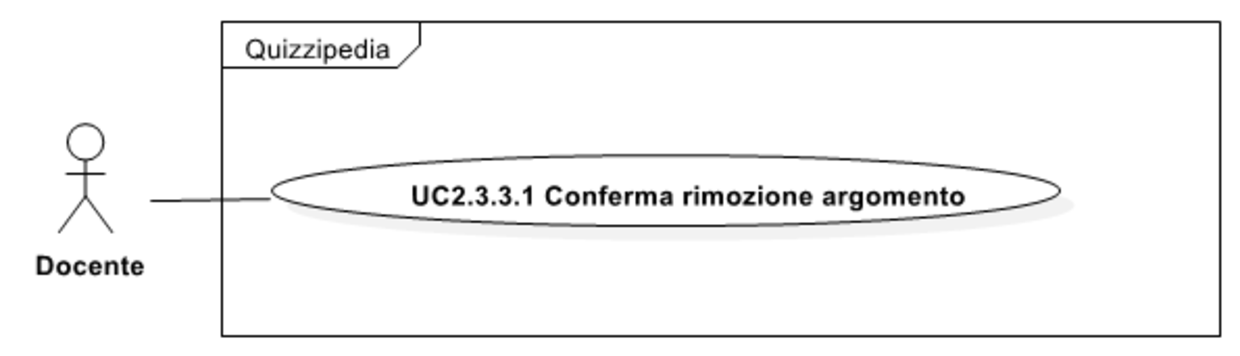
\includegraphics[width=\textwidth]{Img/UC Rimozione argomento.pdf}}
\caption{UC2.3.3 Rimozione argomento}
\end{figure}
\begin{itemize}
\item \textbf{Attori}: Docente.
\item \textbf{Scenario principale}:
\begin{enumerate}
\item Conferma rimozione argomento (UC2.3.3.1).
\end{enumerate}
\item \textbf{Descrizione}: il docente deve poter rimuovere un argomento.
\item \textbf{Precondizione}: il docente è nella gestione degli argomenti e vuole eliminare un argomento.
\item \textbf{Postcondizione}: il docente ha eliminato l’argomento.
\end{itemize}
\subsubsection{UC2.3.3.1 Conferma rimozione argomento}
\begin{itemize}
\item \textbf{Attori}: Docente.
\item \textbf{Scenario principale}: il docente conferma la creazione dell'argomento.
\item \textbf{Descrizione}: il docente deve poter confermare la rimozione dell'argomento.
\item \textbf{Precondizione}: il docente ha selezionato l'argomento da eliminare e deve ancora confermare.
\item \textbf{Postcondizione}: il docente ha confermato l'argomento da eliminare.
\end{itemize}
\subsubsection{UC2.4 Gestione domande}
\begin{figure}[H]
\centering
\noindent\makebox[\textwidth]{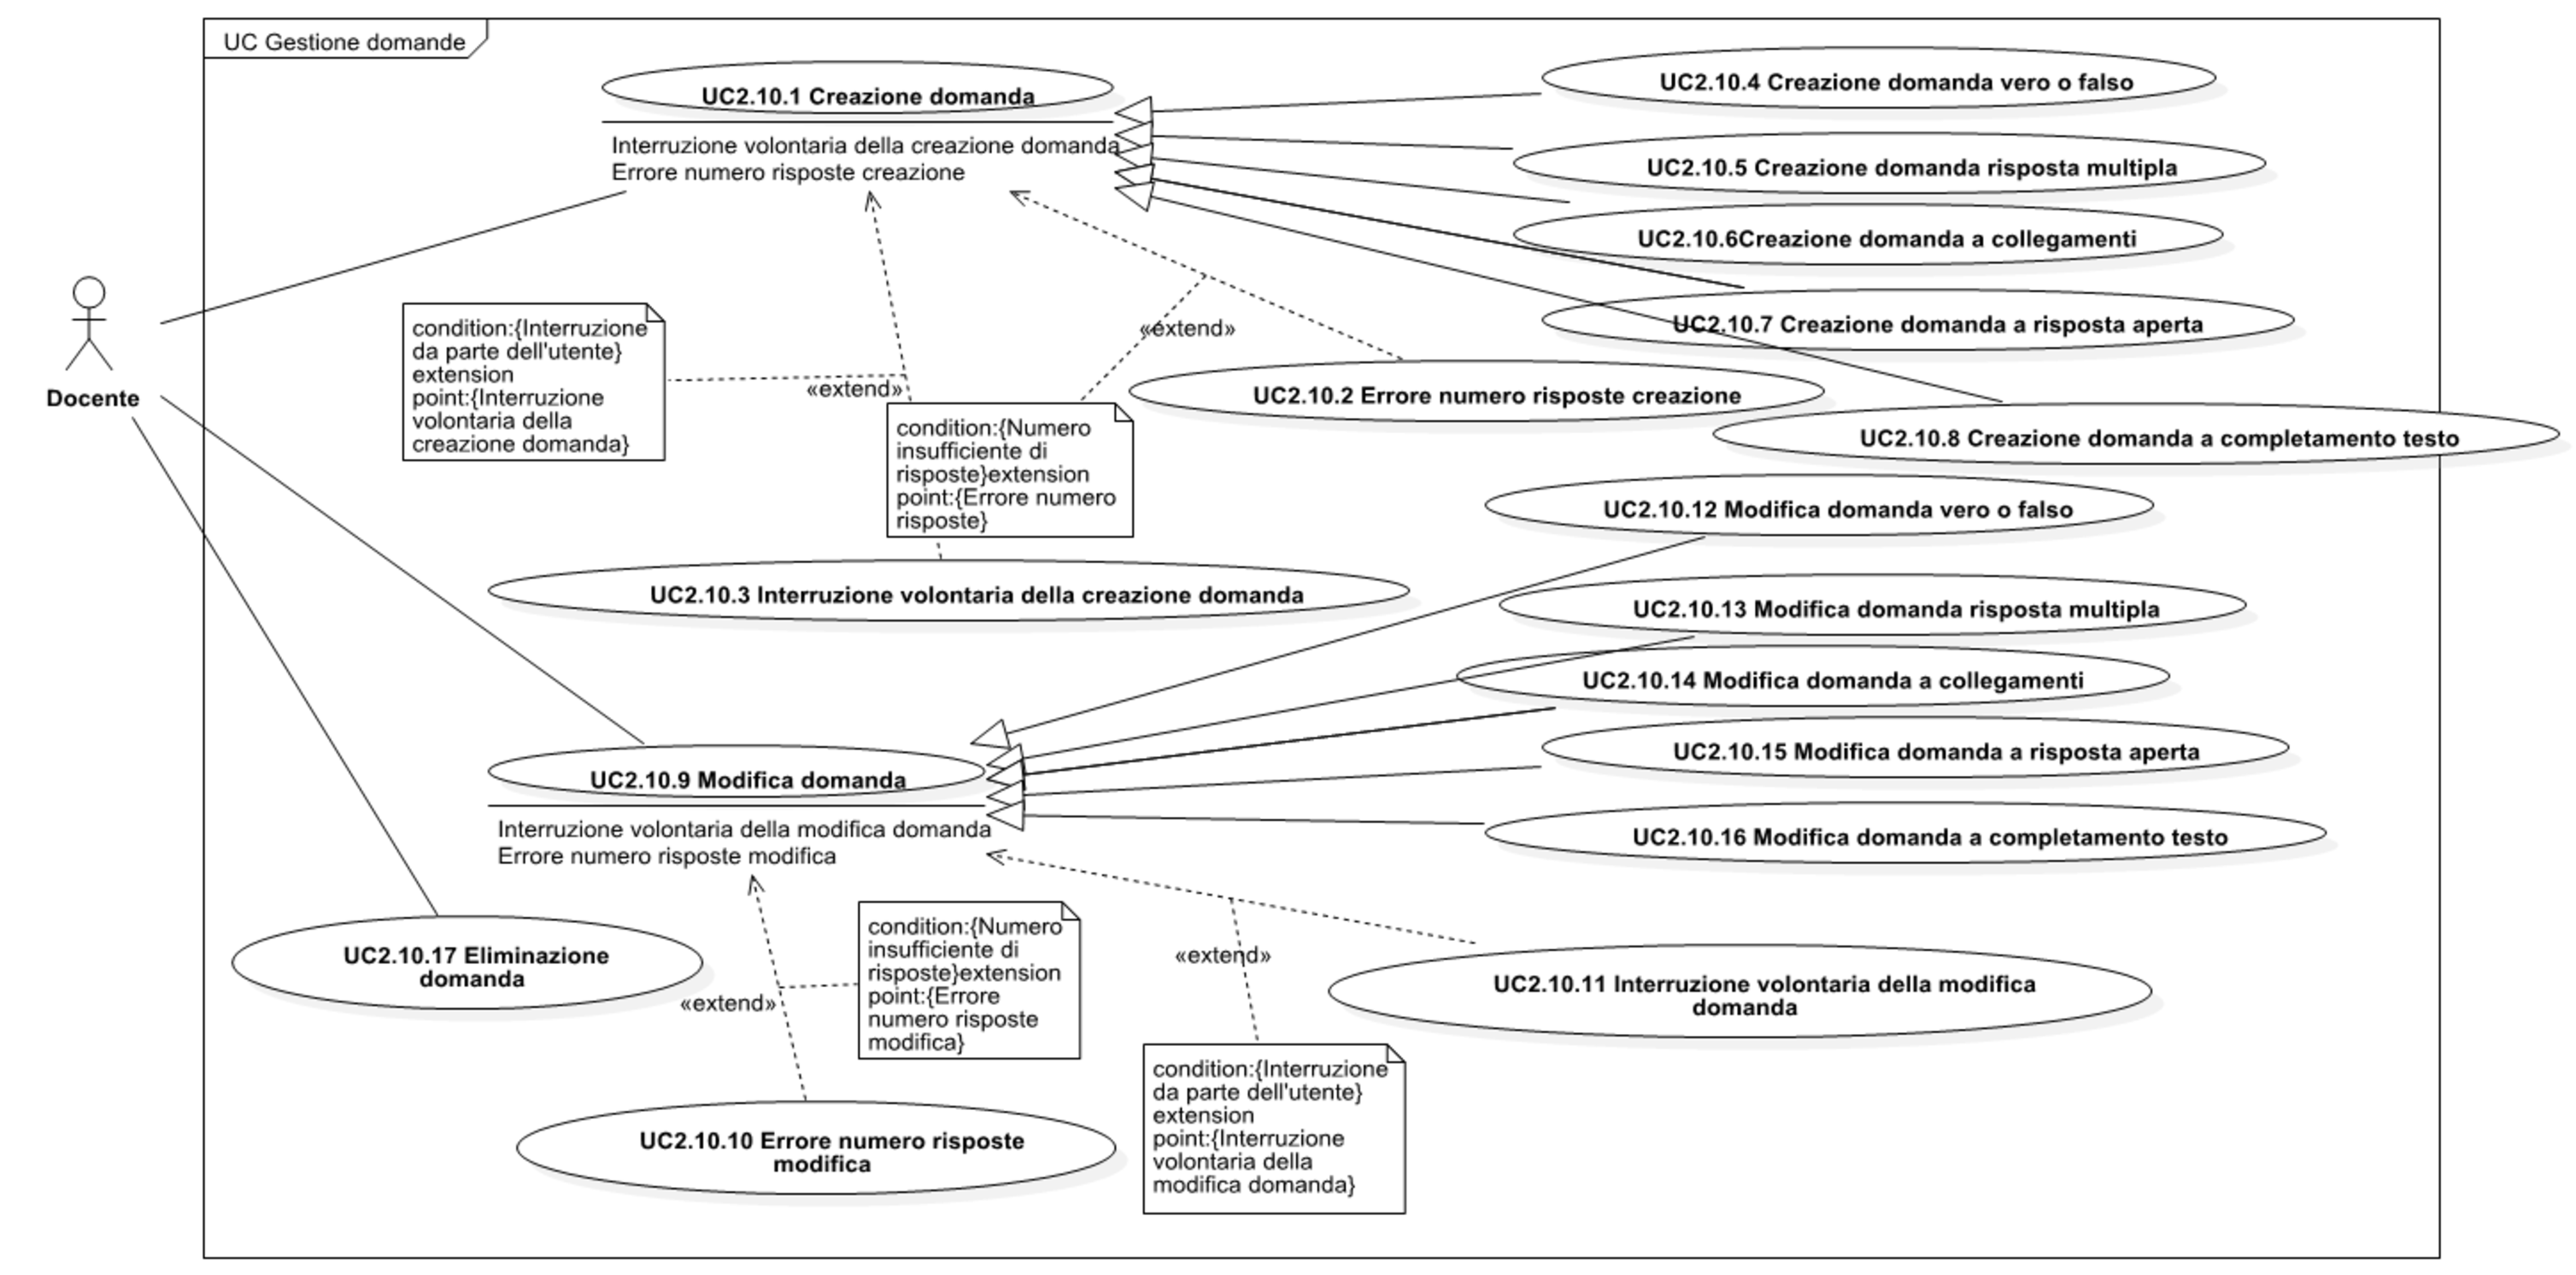
\includegraphics[width=\textwidth]{Img/UC Gestione domande.pdf}}
\caption{UC2.4 Gestione domande}
\end{figure}
\begin{itemize}
\item \textbf{Attori}: Docente.
\item \textbf{Scenario principale}:
\begin{enumerate}
\item Eliminazione domanda (UC2.4.7).
\end{enumerate}
\item \textbf{Descrizione}: il docente deve poter effettuare varie operazioni sulle domande, in particolare deve poter creare nuove domande di vario tipo e modificare o eliminare domande esistenti.
\item \textbf{Precondizione}: il docente è autenticato e desidera gestire le domande.
\item \textbf{Postcondizione}: il docente ha effettuato le operazioni desiderate sulle domande.
\end{itemize}
\subsubsection{UC2.4.7 Eliminazione domanda}
\begin{figure}[H]
\centering
\noindent\makebox[\textwidth]{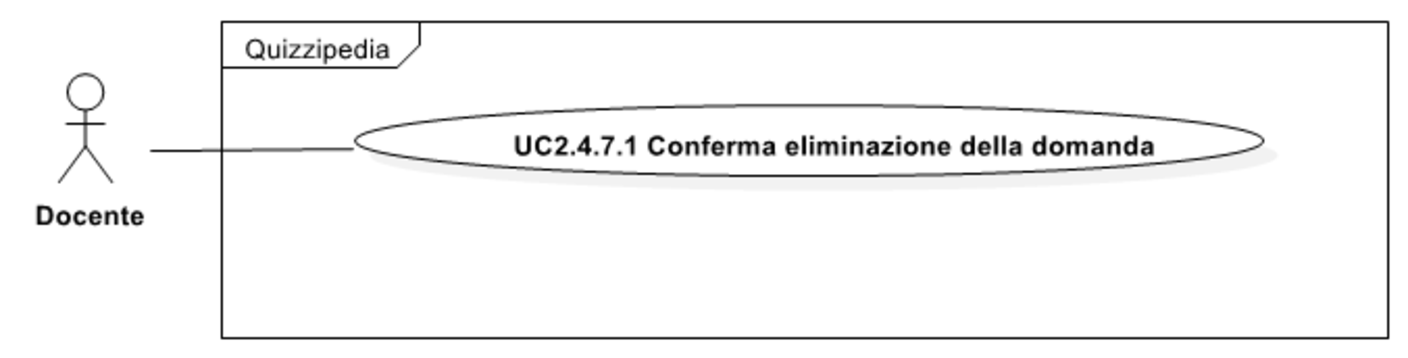
\includegraphics[width=\textwidth]{Img/UC Eliminazione domanda.pdf}}
\caption{UC2.4.7 Eliminazione domanda}
\end{figure}
\begin{itemize}
\item \textbf{Attori}: Docente.
\item \textbf{Scenario principale}:
\begin{enumerate}
\item Conferma eliminazione domanda (UC2.4.7.1).
\end{enumerate}
\item \textbf{Descrizione}: il docente può eliminare una domanda.
\item \textbf{Precondizione}: il docente è autenticato e vuole eliminare  una domanda.
\item \textbf{Postcondizione}: il docente ha eliminato la domanda.
\end{itemize}
\subsubsection{UC2.4.7.1 Conferma eliminazione domanda}
\begin{itemize}
\item \textbf{Attori}: Docente.
\item \textbf{Scenario principale}: il docente conferma l'eliminazione della domanda.
\item \textbf{Descrizione}: il docente conferma l'eliminazione della domanda affinchè l'operazione venga portata a termine. I docenti che hanno precedentemente inserito la domanda nei loro quiz riceveranno una notifica automatica e saranno invitati a controllare i quiz interessati.
\item \textbf{Precondizione}: il docente è autenticato e sta gestendo le domande.
\item \textbf{Postcondizione}: il docente ha confermato l'eliminazione della domanda.
\end{itemize}
\subsubsection{UC2.5 Gestione account}
\begin{figure}[H]
\centering
\noindent\makebox[\textwidth]{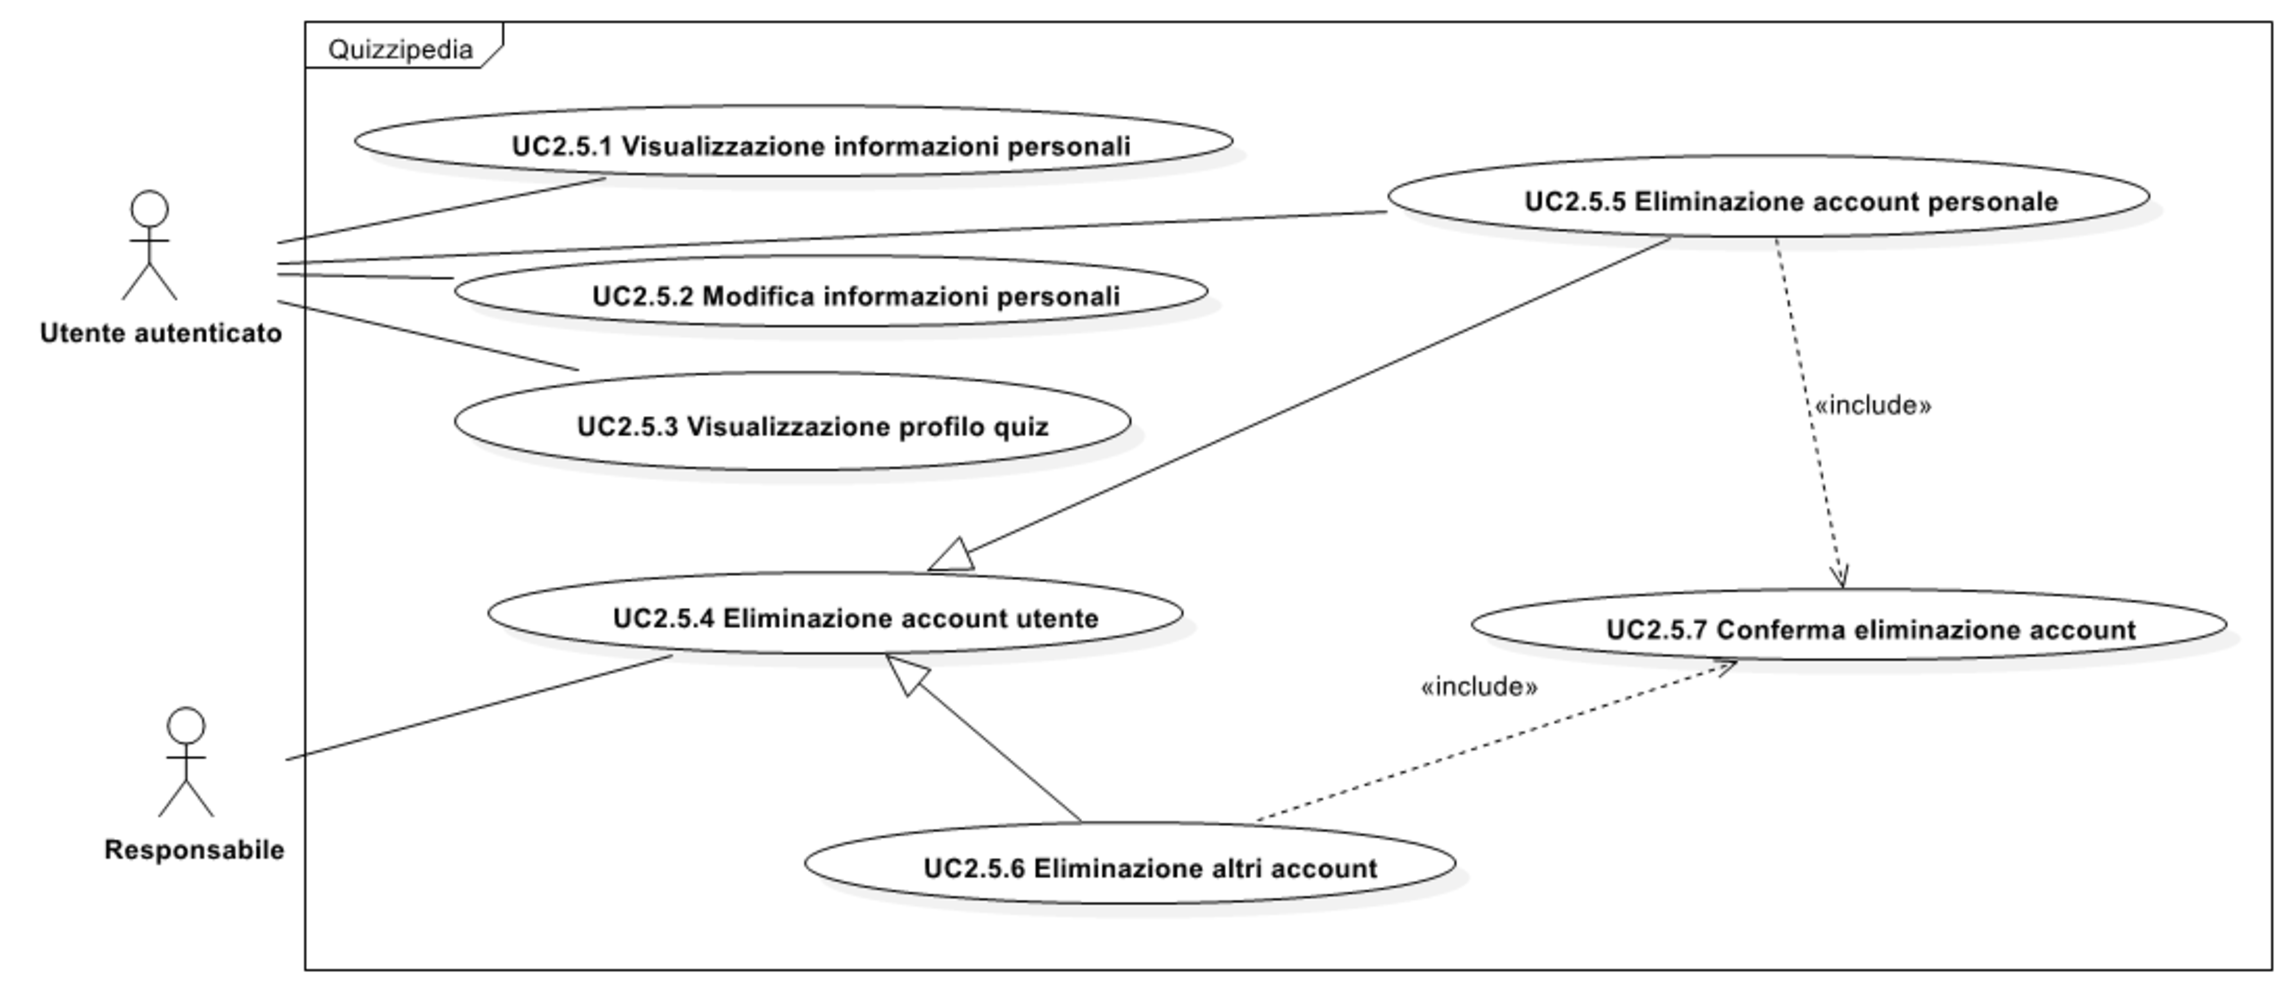
\includegraphics[width=\textwidth]{Img/UC Gestione account.pdf}}
\caption{UC2.5 Gestione account}
\end{figure}
\begin{itemize}
\item \textbf{Attori}: Responsabile, Utente Autenticato.
\item \textbf{Scenario principale}:
\begin{enumerate}
\item Visualizzazione informazioni personali (UC2.5.1);
\item Modifica informazioni personali (UC2.5.2);
\item Visualizzazione profilo quiz (UC2.5.3);
\item Eliminazione account utente (UC2.5.4);
\item Eliminazione account personale (UC2.5.5);
\item Eliminazione altri account (UC2.5.6);
\item Conferma eliminazione account (UC2.5.7);
\item Interruzione volontaria della modifica delle informazioni personali (UC2.5.8).
\end{enumerate}
\item \textbf{Descrizione}: L'utente autenticato può visualizzare e modificare le sue informazioni personali, visualizzare il proprio profilo quiz e la possibilità di eliminare il proprio account. Il responsabile in aggiunta può eliminare gli account degli utenti.
\item \textbf{Precondizione}: il responsabile o un utente autorizzato vuole modificare/visualizzare le informazioni del proprio account.
\item \textbf{Postcondizione}: l'utente autenticato o il responsabile hanno effettuato le modifiche opportune al proprio account.
\end{itemize}
\subsubsection{UC2.5.1 Visualizzazione informazioni personali}
\begin{figure}[H]
\centering
\noindent\makebox[\textwidth]{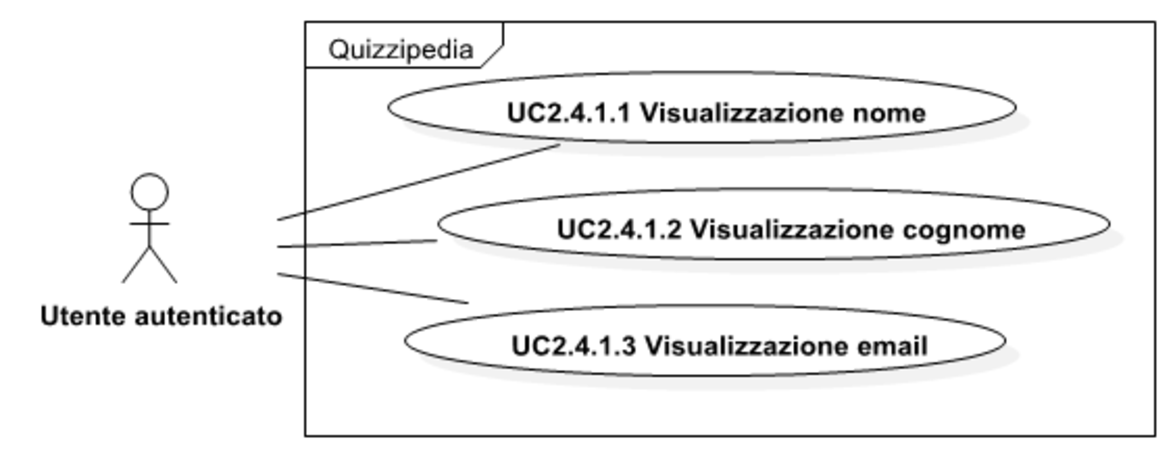
\includegraphics[width=\textwidth]{Img/UC Visualizzazione informazioni personali.pdf}}
\caption{UC2.5.1 Visualizzazione informazioni personali}
\end{figure}
\begin{itemize}
\item \textbf{Attori}: Utente Autenticato.
\item \textbf{Scenario principale}:
\begin{enumerate}
\item Visualizzazione nome (UC2.5.1.1);
\item Visualizzazione cognome (UC2.5.1.2);
\item Visualizzazione email (UC2.5.1.3).
\end{enumerate}
\item \textbf{Descrizione}: l’utente autenticato può visualizzare le sue informazioni personali.
\item \textbf{Precondizione}: l’utente autenticato ha l’accesso alla gestione dell’account.
\item \textbf{Postcondizione}: l’utente autenticato ha visualizzato le sue informazioni personali.
\end{itemize}
\subsubsection{UC2.5.1.1 Visualizzazione nome}
\begin{itemize}
\item \textbf{Attori}: Utente Autenticato.
\item \textbf{Scenario principale}: l'utente autenticato visualizza il proprio nome.
\item \textbf{Descrizione}: l'utente autenticato può visualizzare il suo nome.
\item \textbf{Precondizione}: l'utente è autenticato e sta visualizzando le sue informazioni personali.
\item \textbf{Postcondizione}: l'utente ha visualizzato il proprio nome.
\end{itemize}
\subsubsection{UC2.5.1.2 Visualizzazione cognome}
\begin{itemize}
\item \textbf{Attori}: Utente Autenticato.
\item \textbf{Scenario principale}: l'utente autenticato visualizza il proprio cognome.
\item \textbf{Descrizione}: l'utente autenticato può visualizzare il suo cognome.
\item \textbf{Precondizione}: l'utente è autenticato e sta visualizzando le sue informazioni personali.
\item \textbf{Postcondizione}: l'utente ha visualizzato il proprio cognome.
\end{itemize}
\subsubsection{UC2.5.1.3 Visualizzazione email}
\begin{itemize}
\item \textbf{Attori}: Utente Autenticato.
\item \textbf{Scenario principale}: l'utente autenticato visualizza il proprio indirizzo email.
\item \textbf{Descrizione}: l'utente autenticato può visualizzare la sua email.
\item \textbf{Precondizione}: l'utente è autenticato e sta visualizzando le sue informazioni personali.
\item \textbf{Postcondizione}: l'utente ha visualizzato la propria email.
\end{itemize}
\subsubsection{UC2.5.2 Modifica informazioni personali}
\begin{figure}[H]
\centering
\noindent\makebox[\textwidth]{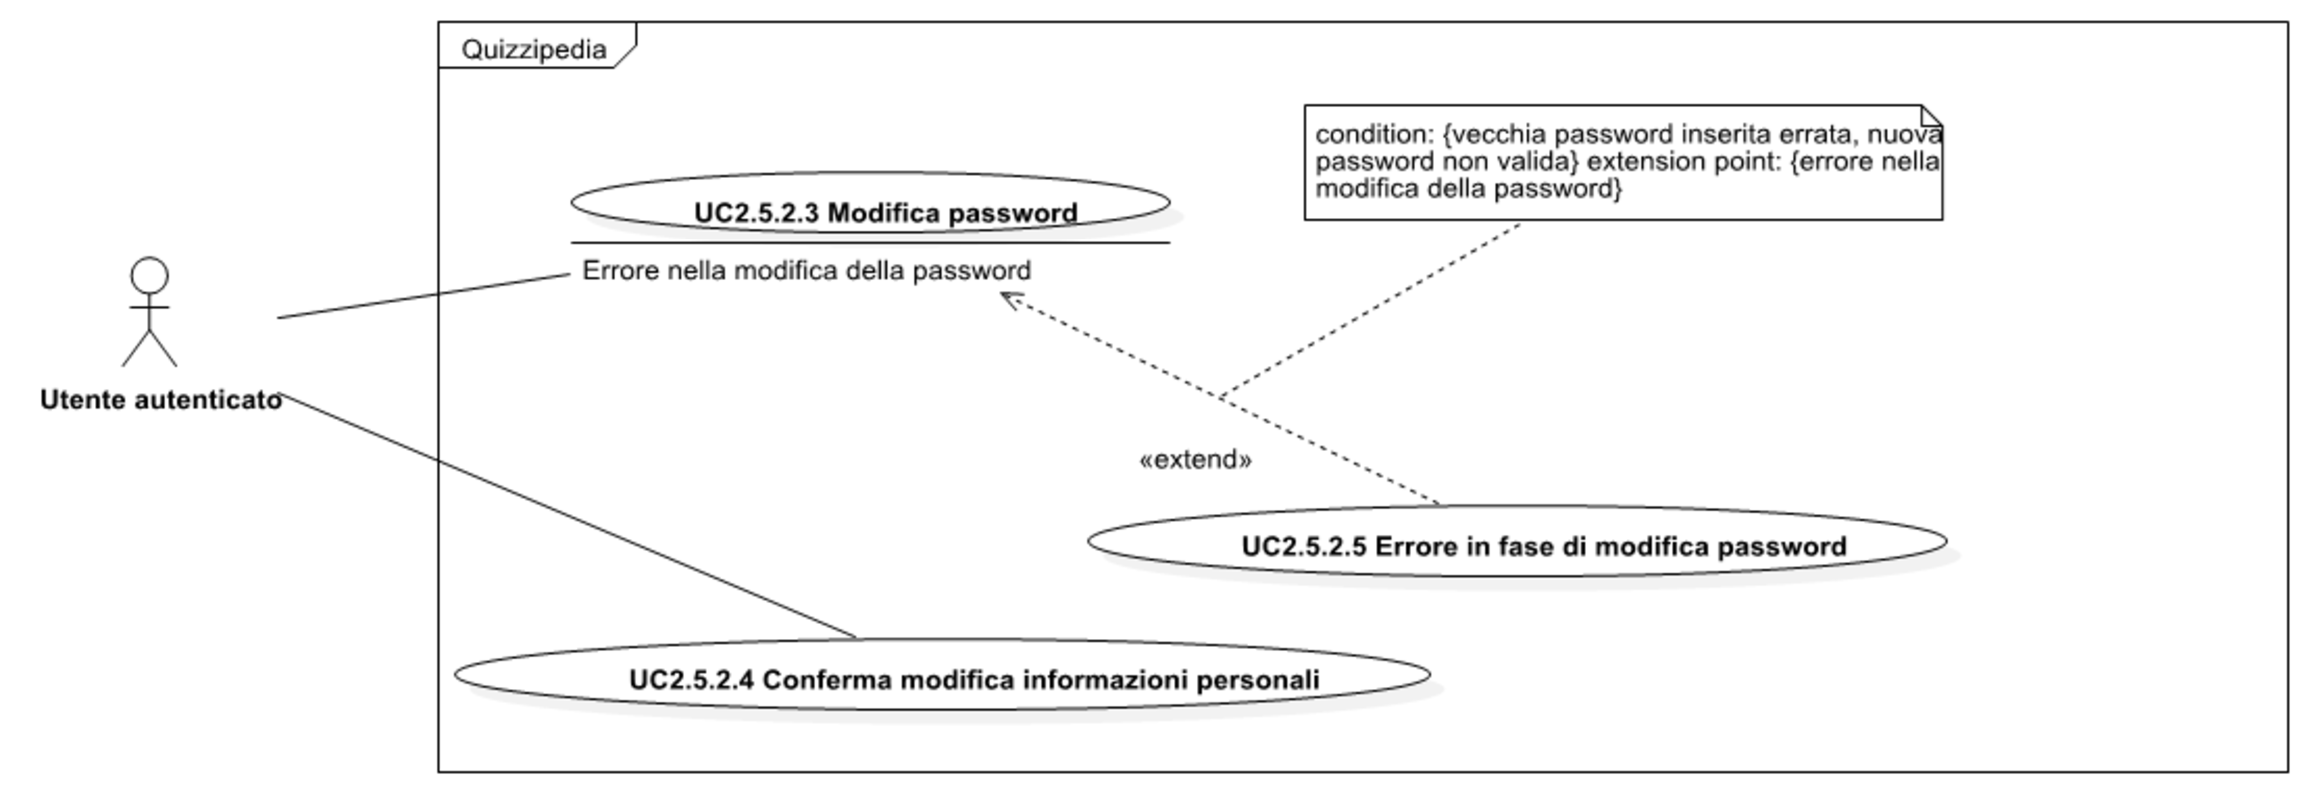
\includegraphics[width=\textwidth]{Img/UC Modifica informazioni personali.pdf}}
\caption{UC2.5.2 Modifica informazioni personali}
\end{figure}
\begin{itemize}
\item \textbf{Attori}: Utente Autenticato.
\item \textbf{Scenario principale}:
\begin{enumerate}
\item Modifica nome (UC2.5.2.1);
\item Modifica cognome (UC2.5.2.2);
\item Modifica password (UC2.5.2.3);
\item Conferma modifica informazioni personali (UC2.5.2.4);
\item Errore modifica password (UC2.5.2.5).
\end{enumerate}
\item \textbf{Estensioni}:
\begin{itemize}
\item Interruzione volontaria della modifica delle informazioni personali (UC2.5.8).
\end{itemize}
\item \textbf{Descrizione}: l'utente autenticato vuole modificare le sue informazioni personali.
\item \textbf{Precondizione}: l'utente autenticato può modificare le sue informazioni personali.
\item \textbf{Postcondizione}: l'utente ha modificato le sue informazioni personali.
\end{itemize}
\subsubsection{UC2.5.2.1 Modifica nome}
\begin{itemize}
\item \textbf{Attori}: Utente Autenticato.
\item \textbf{Scenario principale}: l'utente autenticato modifica il suo nome.
\item \textbf{Descrizione}: l'utente autenticato può modificare il suo nome.
\item \textbf{Precondizione}: l'utente autenticato modifica le sue informazioni personali.
\item \textbf{Postcondizione}: l'utente ha modificato il suo nome.
\end{itemize}
\subsubsection{UC2.5.2.2 Modifica cognome}
\begin{itemize}
\item \textbf{Attori}: Utente Autenticato.
\item \textbf{Scenario principale}: l'utente autenticato modifica il suo cognome.
\item \textbf{Descrizione}: l'utente autenticato può modificare il suo cognome.
\item \textbf{Precondizione}: l'utente autenticato modifica le sue informazioni personali.
\item \textbf{Postcondizione}: l'utente ha modificato il suo cognome.
\end{itemize}
\subsubsection{UC2.5.2.3 Modifica password}
\begin{figure}[H]
\centering
\noindent\makebox[\textwidth]{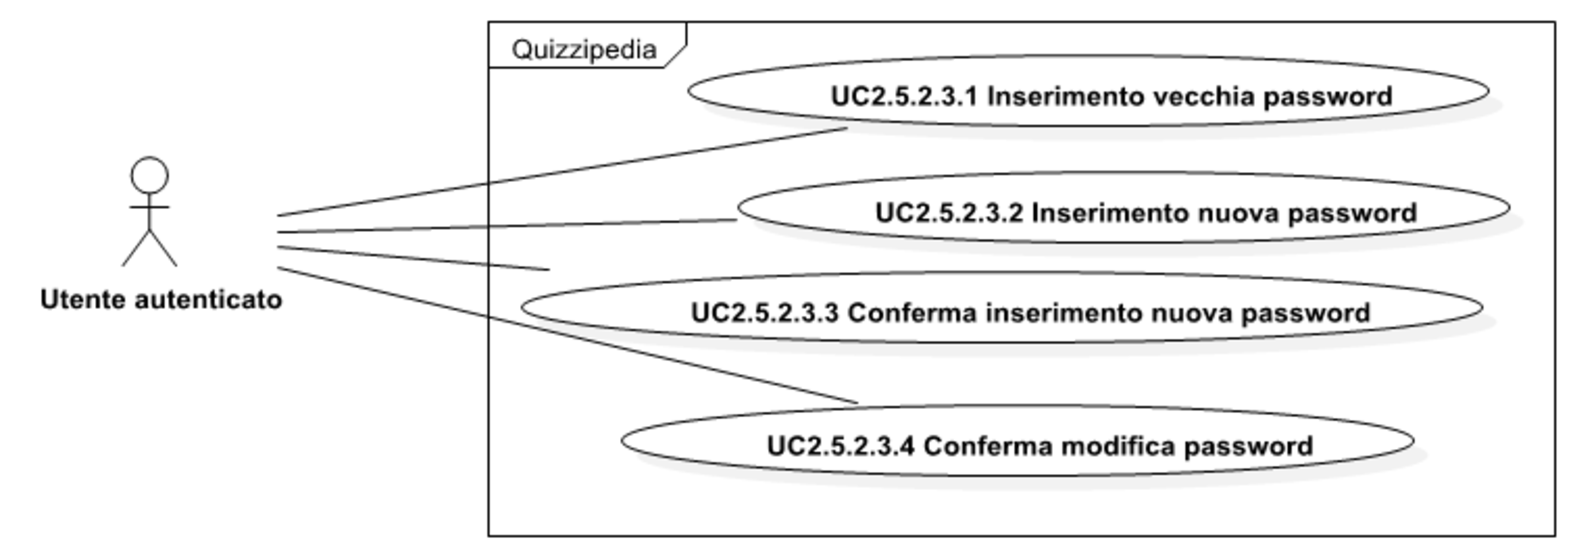
\includegraphics[width=\textwidth]{Img/UC Modifica password.pdf}}
\caption{UC2.5.2.3 Modifica password}
\end{figure}
\begin{itemize}
\item \textbf{Attori}: Utente Autenticato.
\item \textbf{Scenario principale}:
\begin{enumerate}
\item Inserimento vecchia password (UC2.5.2.3.1);
\item Inserimento nuova password (UC2.5.2.3.2);
\item Conferma inserimento nuova password (UC2.5.2.3.3);
\item Conferma modifica password (UC2.5.2.3.4).
\end{enumerate}
\item \textbf{Estensioni}:
\begin{itemize}
\item Errore modifica password (UC2.5.2.5).
\end{itemize}
\item \textbf{Descrizione}: l'utente autenticato può modificare la sua password.
\item \textbf{Precondizione}: l'utente autenticato modifica le sue informazioni personali.
\item \textbf{Postcondizione}: l'utente ha modificato la sua password.
\end{itemize}
\subsubsection{UC2.5.2.3.1 Inserimento vecchia password}
\begin{itemize}
\item \textbf{Attori}: Utente Autenticato.
\item \textbf{Scenario principale}: l'utente autenticato inserisce la sua vecchia password.
\item \textbf{Descrizione}: la modifica della password richiede l'inserimento della password corrente o di una password temporanea.
\item \textbf{Precondizione}: l'utente autenticato ha deciso di modificare la password e deve ancora inserire la vecchia password.
\item \textbf{Postcondizione}: l'utente autenticato ha inserito la vecchia password.
\end{itemize}
\subsubsection{UC2.5.2.3.2 Inserimento nuova password}
\begin{itemize}
\item \textbf{Attori}: Utente Autenticato.
\item \textbf{Scenario principale}: l'utente autenticato inserisce la nuova password.
\item \textbf{Descrizione}: la modifica della password richiede l'inserimento della nuova password.
\item \textbf{Precondizione}: l'utente autenticato ha deciso di modificare la password e deve ancora inserire la nuova password.
\item \textbf{Postcondizione}: l'utente autenticato ha inserito la nuova password.
\end{itemize}
\subsubsection{UC2.5.2.3.3 Conferma inserimento nuova password}
\begin{itemize}
\item \textbf{Attori}: Utente Autenticato.
\item \textbf{Scenario principale}: l'utente autenticato conferma l'inserimento della nuova password.
\item \textbf{Descrizione}: la modifica della password richiede la conferma dell'inserimento della nuova password.
\item \textbf{Precondizione}: l'utente autenticato ha deciso di modificare la password e deve ancora confermare l'inserimento della nuova password.
\item \textbf{Postcondizione}: l'utente autenticato ha confermato l'inserimento della nuova password.
\end{itemize}
\subsubsection{UC2.5.2.3.4 Conferma modifica password}
\begin{itemize}
\item \textbf{Attori}: Utente Autenticato.
\item \textbf{Scenario principale}: l'utente autenticato conferma la modifica della password.
\item \textbf{Descrizione}: La modifica della password richiede la conferma della modifica password.
\item \textbf{Precondizione}: l'utente autenticato ha inserito i campi necessari e deve ancora confermare la modifica della password.
\item \textbf{Postcondizione}: l'utente autenticato ha confermato la modifica della password.
\end{itemize}
\subsubsection{UC2.5.2.4 Conferma modifica informazioni personali}
\begin{itemize}
\item \textbf{Attori}: Utente Autenticato.
\item \textbf{Scenario principale}: l'utente autenticato conferma la modifica delle informazioni personali.
\item \textbf{Descrizione}: l'utente autenticato deve confermare le modifiche effettuate.
\item \textbf{Precondizione}: l'utente autenticato ha modificato qualche informazione personale.
\item \textbf{Postcondizione}: l'utente autenticato ha confermato  le nuove informazioni personali.
\end{itemize}
\subsubsection{UC2.5.2.5 Errore modifica password}
\begin{itemize}
\item \textbf{Attori}: Utente Autenticato.
\item \textbf{Scenario principale}: l'utente visualizza il messaggio di errore.
\item \textbf{Descrizione}: si è verificato un errore durante la modifica della password.
\item \textbf{Precondizione}: l'utente autenticato ha inserito una password non valida.
\item \textbf{Postcondizione}: l'utente visualizza un messaggio di errore.
\end{itemize}
\subsubsection{UC2.5.3 Visualizzazione profilo quiz}
\begin{itemize}
\item \textbf{Attori}: Utente Autenticato.
\item \textbf{Scenario principale}: l'utente autenticato visualizza il suo storico dei quiz e le risposte.
\item \textbf{Descrizione}: l'utente autenticato può visualizzare il suo storico dei quiz e rivedere le risposte date.
\item \textbf{Precondizione}: l'utente autenticato può visualizzare lo storico dei quiz.
\item \textbf{Postcondizione}: l'utente ha visualizzato il suo profilo quiz.
\end{itemize}
\subsubsection{UC2.5.4 Eliminazione account utente}
\begin{itemize}
\item \textbf{Attori}: Responsabile.
\item \textbf{Scenario principale}: il responsabile elimina l'account desiderato.
\item \textbf{Generalizzazioni}:
\begin{itemize}
\item Eliminazione account personale (UC2.5.5);
\item Eliminazione altri account (UC2.5.6).
\end{itemize}
\item \textbf{Descrizione}: il responsabile può eliminare il proprio account e tutti gli account degli utenti.
\item \textbf{Precondizione}: il responsabile ha il permesso di eliminare gli account utente.
\item \textbf{Postcondizione}: il responsabile ha eliminato un account di un utente o ha eliminato il suo account.
\end{itemize}
\subsubsection{UC2.5.5 Eliminazione account personale}
\begin{itemize}
\item \textbf{Attori}: Responsabile, Utente Autenticato.
\item \textbf{Scenario principale}:
\begin{enumerate}
\item Conferma eliminazione account personale (UC2.5.5.1).
\end{enumerate}
\item \textbf{Descrizione}: l’utente autenticato e il responsabile possono cancellare il proprio account personale.
\item \textbf{Precondizione}: l’utente autenticato e il responsabile hanno i permessi per cancellare l’account.
\item \textbf{Postcondizione}: l’utente autenticato e il responsabile hanno selezionato il loro account per l’eliminazione.
\item \textbf{Specializzazione di}:
\begin{enumerate}
\item Eliminazione account utente (UC2.5.4).
\end{enumerate}
\end{itemize}
\subsubsection{UC2.5.5.1 Conferma eliminazione account personale}
\begin{itemize}
\item \textbf{Attori}: Utente Autenticato.
\item \textbf{Scenario principale}: l'utente conferma l'eliminazione del proprio account.
\item \textbf{Descrizione}: L'utente deve confermare l'eliminazione del proprio account.
\item \textbf{Precondizione}: L'utente si trova nella pagina di eliminazione del proprio account.
\item \textbf{Postcondizione}: L'utente ha confermato l'eliminazione del proprio account.
\end{itemize}
\subsubsection{UC2.5.6 Eliminazione altri account}
\begin{itemize}
\item \textbf{Attori}: Responsabile.
\item \textbf{Scenario principale}:
\begin{enumerate}
\item Conferma eliminazione altri account (UC2.5.6.1).
\end{enumerate}
\item \textbf{Descrizione}: il responsabile può cancellare gli account degli altri utenti.
\item \textbf{Precondizione}: il responsabile ha i permessi di eliminazione altri account.
\item \textbf{Postcondizione}: il responsabile ha selezionato l’account da eliminare.
\item \textbf{Specializzazione di}:
\begin{enumerate}
\item Eliminazione account utente (UC2.5.4).
\end{enumerate}
\end{itemize}
\subsubsection{UC2.5.6.1 Conferma eliminazione altri account}
\begin{itemize}
\item \textbf{Attori}: Responsabile.
\item \textbf{Scenario principale}: il responsabile conferma l'eliminazione dell'account.
\item \textbf{Descrizione}: Il responsabile deve confermare l'eliminazione dell'account di un altro utente.
\item \textbf{Precondizione}: Il responsabile si trova nella pagina di eliminazione di altri account.
\item \textbf{Postcondizione}: Il responsabile ha confermato l'eliminazione dell'account dell'utente.
\end{itemize}
\subsubsection{UC2.5.7 Conferma eliminazione account}
\begin{itemize}
\item \textbf{Attori}: Responsabile, Utente Autenticato.
\item \textbf{Scenario principale}: l'utente conferma l'eliminazione dell'account.
\item \textbf{Descrizione}: l'utente autenticato e il responsabile confermano l'eliminazione vera e propria dell'account precedentemente selezionato.
\item \textbf{Precondizione}: l'utente autenticato o il responsabile hanno precedentemente selezionato un account da eliminare.
\item \textbf{Postcondizione}: l'account precedentemente selezionato è stato eliminato definitivamente.
\end{itemize}
\subsubsection{UC2.5.8 Interruzione volontaria della modifica delle informazioni personali}
\begin{itemize}
\item \textbf{Attori}: Utente Autenticato.
\item \textbf{Scenario principale}: l'utente interrompe la modifica delle informazioni personali.
\item \textbf{Descrizione}: l'utente può interrompere la modifica delle informazioni personali.
\item \textbf{Precondizione}: l'utente sta modificando le proprie informazioni personali.
\item \textbf{Postcondizione}: l'utente non ha completato la modifica delle informazioni personali.
\end{itemize}
\subsubsection{UC2.6 Richiesta accettazione}
\begin{figure}[H]
\centering
\noindent\makebox[\textwidth]{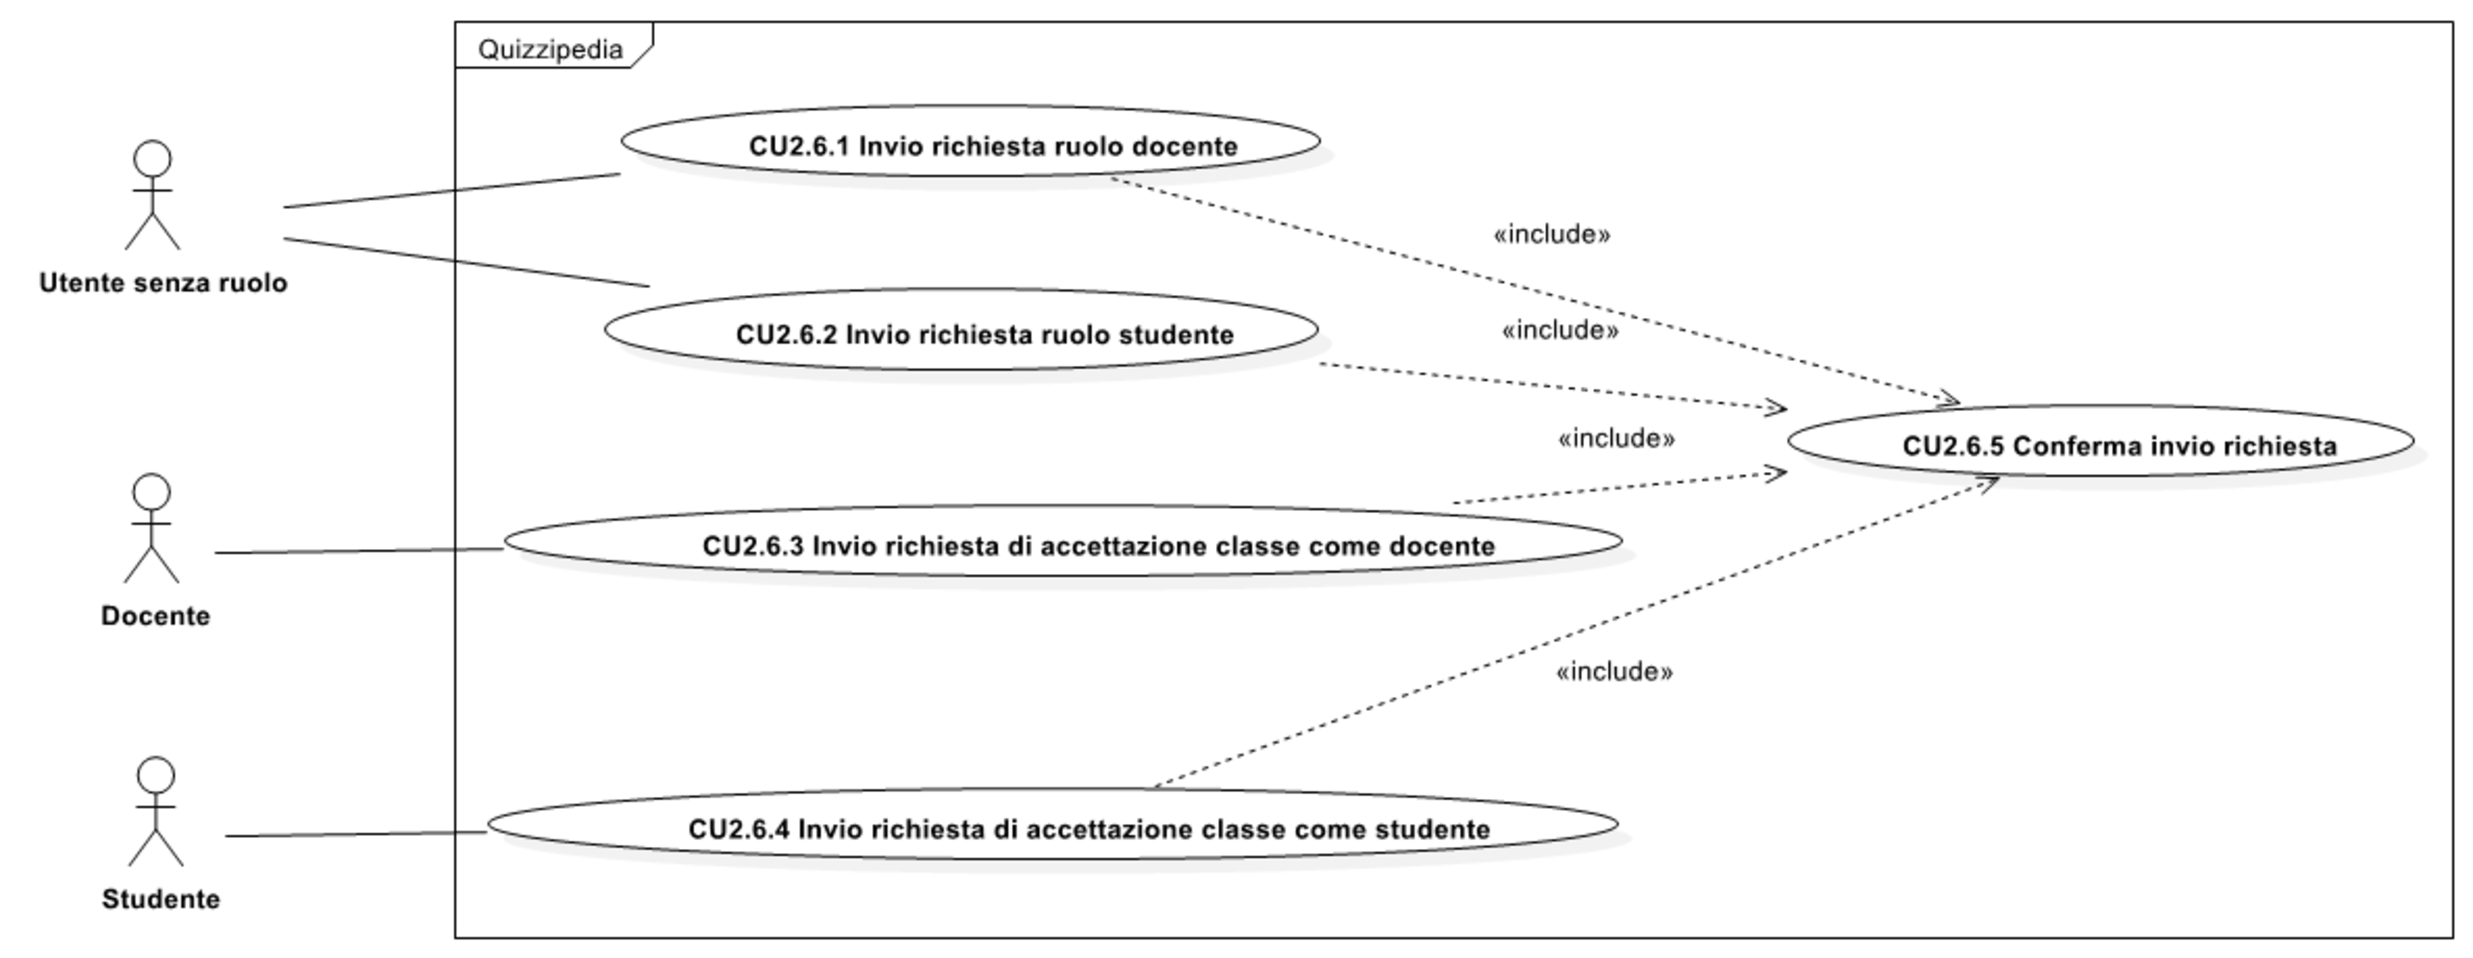
\includegraphics[width=\textwidth]{Img/UC Richiesta accettazione.pdf}}
\caption{UC2.6 Richiesta accettazione}
\end{figure}
\begin{itemize}
\item \textbf{Attori}: Docente, Studente, Utente senza Ruolo.
\item \textbf{Scenario principale}:
\begin{enumerate}
\item Invio richiesta ruolo docente (UC2.6.1);
\item Invio richiesta ruolo studente (UC2.6.2);
\item Invio richiesta di accettazione classe come docente (UC2.6.3);
\item Invio richiesta di accettazione classe come studente (UC2.6.4);
\item Conferma invio richiesta (UC2.6.5).
\end{enumerate}
\item \textbf{Descrizione}: l’utente senza ruolo invia una richiesta per essere studente o docente, mentre studente e docente inviano una richiesta di accettazione per essere inseriti in una determinata classe.
\item \textbf{Precondizione}: utente senza ruolo, studente e docente possono inviare richieste di accettazione.
\item \textbf{Postcondizione}: è stata inviata una richesta d’accettazione e sarà notificata al responsabile.
\end{itemize}
\subsubsection{UC2.6.1 Invio richiesta ruolo docente}
\begin{itemize}
\item \textbf{Attori}: Utente senza Ruolo.
\item \textbf{Scenario principale}: l'utente invia la richiesta di ruolo 'docente'.
\item \textbf{Inclusioni}:
\begin{itemize}
\item Conferma invio richiesta (UC2.6.5).
\end{itemize}
\item \textbf{Descrizione}: l'utente senza ruolo compila la richiesta per acquisire il ruolo di docente che sarà successivamente accettata  o rifiutata dal responsabile.
\item \textbf{Precondizione}: l'utente deve essere un utente senza ruolo.
\item \textbf{Postcondizione}: l'utente senza ruolo ha compilato la richiesta di acquisizione ruolo docente.
\end{itemize}
\subsubsection{UC2.6.2 Invio richiesta ruolo studente}
\begin{itemize}
\item \textbf{Attori}: Utente senza Ruolo.
\item \textbf{Scenario principale}: l'utente invia la richiesta di ruolo 'studente'.
\item \textbf{Inclusioni}:
\begin{itemize}
\item Conferma invio richiesta (UC2.6.5).
\end{itemize}
\item \textbf{Descrizione}: l'utente senza ruolo compila la richiesta per acquisire il ruolo di studente che sarà successivamente accettata o rifiutata dal responsabile.
\item \textbf{Precondizione}: l'utente deve essere un utente senza ruolo.
\item \textbf{Postcondizione}: l'utente senza ruolo ha compilato la richiesta di acquisizione ruolo studente.
\end{itemize}
\subsubsection{UC2.6.3 Invio richiesta di accettazione classe come docente}
\begin{itemize}
\item \textbf{Attori}: Docente.
\item \textbf{Scenario principale}:
\begin{enumerate}
\item Inserimento nome classe (UC2.6.3.1).
\end{enumerate}
\item \textbf{Inclusioni}:
\begin{itemize}
\item Conferma invio richiesta (UC2.6.5).
\end{itemize}
\item \textbf{Descrizione}: il docente invia una richiesta al responsabile con il nome della classe per avere il permesso di essere inserito nella classe indicata.
\item \textbf{Precondizione}: il docente ha il permesso di inviare la richiesta.
\item \textbf{Postcondizione}: il docente ha compilato la richiesta.
\end{itemize}
\subsubsection{UC2.6.3.1 Inserimento nome classe}
\begin{itemize}
\item \textbf{Attori}: Docente.
\item \textbf{Scenario principale}: il docente seleziona il nome della classe.
\item \textbf{Descrizione}: il docente deve poter seleziona il nome della classe alla quale vuole essere inserito.
\item \textbf{Precondizione}: il docente è nella fase di invio richiesta di accettazione classe come docente.
\item \textbf{Postcondizione}: il docente ha selezionato il nome della classe.
\end{itemize}
\subsubsection{UC2.6.4 Invio richiesta di accettazione classe come studente}
\begin{itemize}
\item \textbf{Attori}: Studente.
\item \textbf{Scenario principale}:
\begin{enumerate}
\item Inserimento nome classe (UC2.6.4.1).
\end{enumerate}
\item \textbf{Inclusioni}:
\begin{itemize}
\item Conferma invio richiesta (UC2.6.5).
\end{itemize}
\item \textbf{Descrizione}: lo studente invia una richiesta al responsabile con il nome della classe per avere il permesso di essere inserito nella classe indicata.
\item \textbf{Precondizione}: lo studente ha il permesso di inviare questa richiesta.
\item \textbf{Postcondizione}: lo studente ha compilato la richiesta.
\end{itemize}
\subsubsection{UC2.6.4.1 Inserimento nome classe}
\begin{itemize}
\item \textbf{Attori}: Studente.
\item \textbf{Scenario principale}: l'utente seleziona il nome della classe.
\item \textbf{Descrizione}: lo studente deve poter selezionare il nome della classe alla quale vuole essere inserito.
\item \textbf{Precondizione}: lo studente è nella fase di invio di richiesta di accettazione classe come studente.
\item \textbf{Postcondizione}: lo studente ha selezionato il nome della classe.
\end{itemize}
\subsubsection{UC2.6.5 Conferma invio richiesta}
\begin{itemize}
\item \textbf{Attori}: Docente, Studente, Utente senza Ruolo.
\item \textbf{Scenario principale}: l'utente conferma l'invio della richiesta.
\item \textbf{Descrizione}: l'utente senza ruolo, studente e docente devono poter confermare l'invio della richiesta  precedentemente compilata.
\item \textbf{Precondizione}: l'utente senza ruolo, docente, studente hanno compilato la richiesta appropriata.
\item \textbf{Postcondizione}: la richiesta è stata inviata al responsabile con successo.
\end{itemize}
\subsubsection{UC2.7 Visualizzazione statistiche}
\begin{figure}[H]
\centering
\noindent\makebox[\textwidth]{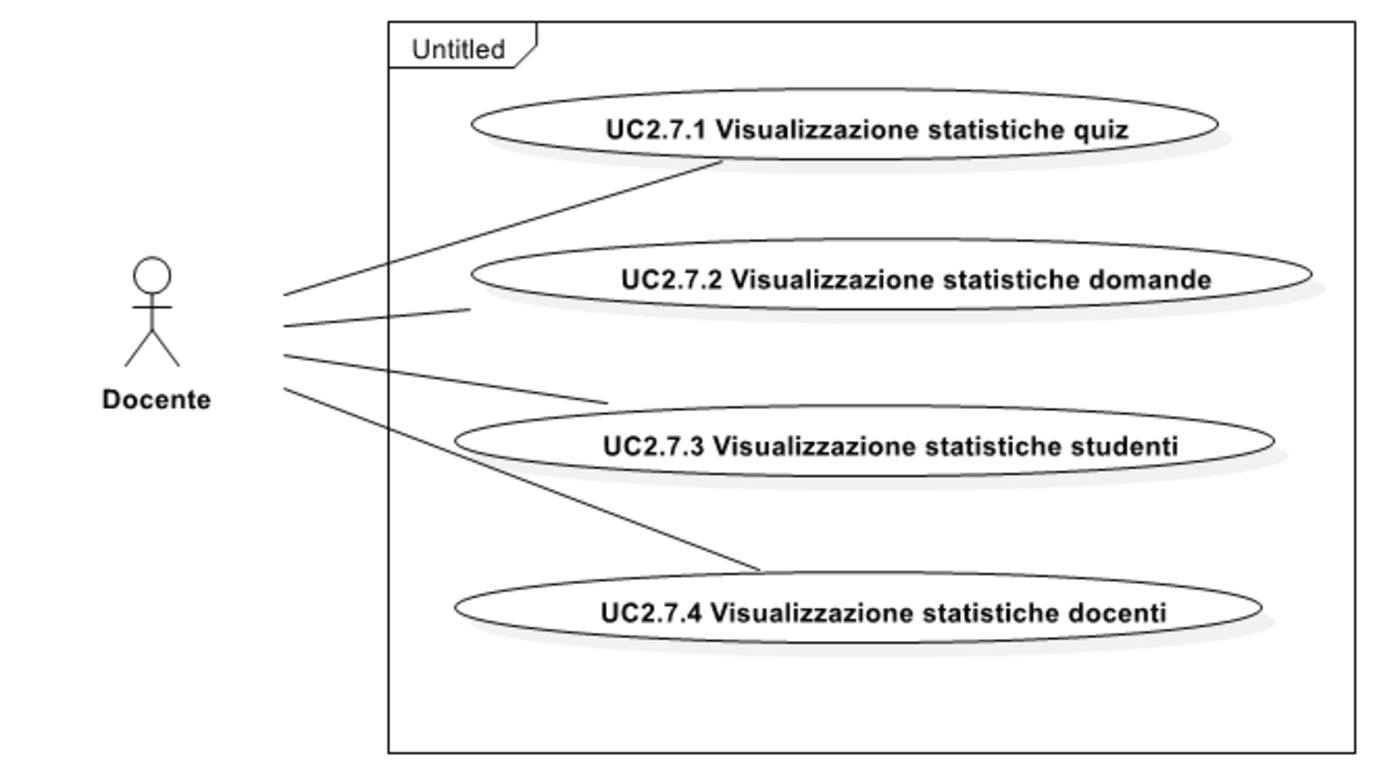
\includegraphics[width=\textwidth]{Img/UC Visualizzazione statistiche.pdf}}
\caption{UC2.7 Visualizzazione statistiche}
\end{figure}
\begin{itemize}
\item \textbf{Attori}: Docente.
\item \textbf{Scenario principale}:
\begin{enumerate}
\item Visualizzazione statistiche quiz (UC2.7.1);
\item Visualizzazione statistiche domande (UC2.7.2);
\item Visualizzazione statistiche studenti (UC2.7.3);
\item Visualizzazione statistiche docenti (UC2.7.4).
\end{enumerate}
\item \textbf{Descrizione}: il docente deve poter visualizzare statistiche di vario tipo relative a quiz, domande, studenti e altri docenti.
\item \textbf{Precondizione}: il docente è autenticato nel sistema e desidera visualizzare le statistiche.
\item \textbf{Postcondizione}: il docente ha visualizzato le statistiche.
\end{itemize}
\subsubsection{UC2.7.1 Visualizzazione statistiche quiz}
\begin{figure}[H]
\centering
\noindent\makebox[\textwidth]{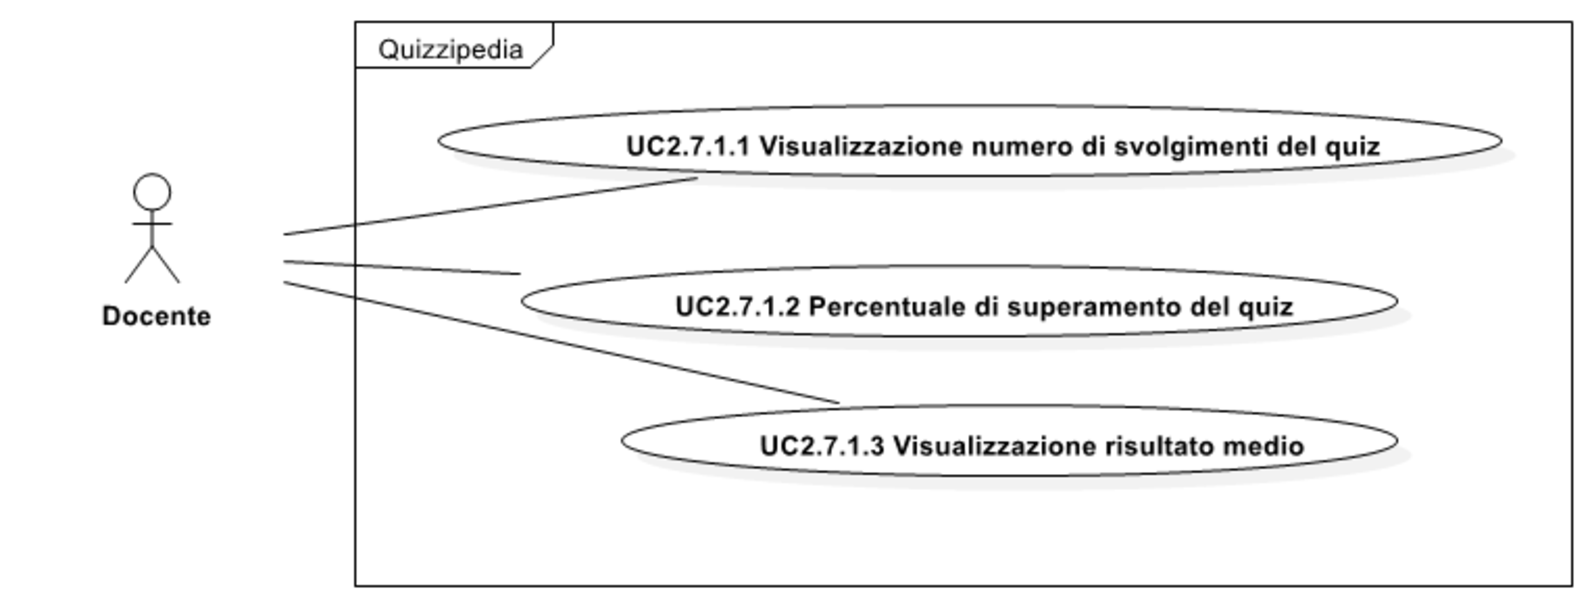
\includegraphics[width=\textwidth]{Img/UC Visualizzazione statistiche quiz.pdf}}
\caption{UC2.7.1 Visualizzazione statistiche quiz}
\end{figure}
\begin{itemize}
\item \textbf{Attori}: Docente.
\item \textbf{Scenario principale}:
\begin{enumerate}
\item Visualizzazione numero di svolgimenti (UC2.7.1.1);
\item Visualizzazione percentuale di superamento del quiz (UC2.7.1.2);
\item Visualizzazione risultato medio (UC2.7.1.3).
\end{enumerate}
\item \textbf{Descrizione}: il docente deve poter visualizzare statistiche legate ai quiz.
\item \textbf{Precondizione}: il docente è autenticato nel sistema e desidera visualizzare le statistiche legate ai quiz.
\item \textbf{Postcondizione}: il docente ha visualizzato le statistiche legate ai quiz.
\end{itemize}
\subsubsection{UC2.7.1.1 Visualizzazione numero di svolgimenti}
\begin{itemize}
\item \textbf{Attori}: Docente.
\item \textbf{Scenario principale}: il docente visualizza il numero di volte in cui un quiz è stato svolto.
\item \textbf{Descrizione}: il docente deve poter visualizzare il numero di volte in cui un quiz è stato svolto.
\item \textbf{Precondizione}: il docente ha deciso di visualizzare le statistiche legate ai quiz.
\item \textbf{Postcondizione}: il docente ha visualizzato il numero di svolgimenti di un quiz.
\end{itemize}
\subsubsection{UC2.7.1.2 Visualizzazione percentuale di superamento del quiz}
\begin{itemize}
\item \textbf{Attori}: Docente.
\item \textbf{Scenario principale}: il docente visualizza la percentuale di studenti che hanno svolto il quiz con esito positivo.
\item \textbf{Descrizione}: il docente deve poter visualizzare la percentuale di studenti che hanno svolto il quiz con esito positivo.
\item \textbf{Precondizione}: il docente ha deciso di visualizzare le statistiche legate ai quiz.
\item \textbf{Postcondizione}: il docente ha visualizzato la percentuale di superamento di un quiz.
\end{itemize}
\subsubsection{UC2.7.1.3 Visualizzazione risultato medio}
\begin{itemize}
\item \textbf{Attori}: Docente.
\item \textbf{Scenario principale}: il docente visualizza il risultato medio ottenuto dagli utenti che hanno svolto il quiz.
\item \textbf{Descrizione}: il docente deve poter visualizzare il risultato medio ottenuto dagli utenti che hanno svolto il quiz.
\item \textbf{Precondizione}: il docente ha deciso di visualizzare le statistiche legate ai quiz.
\item \textbf{Postcondizione}: il docente ha visualizzato il risultato medio di un quiz.
\end{itemize}
\subsubsection{UC2.7.2 Visualizzazione statistiche domande}
\begin{figure}[H]
\centering
\noindent\makebox[\textwidth]{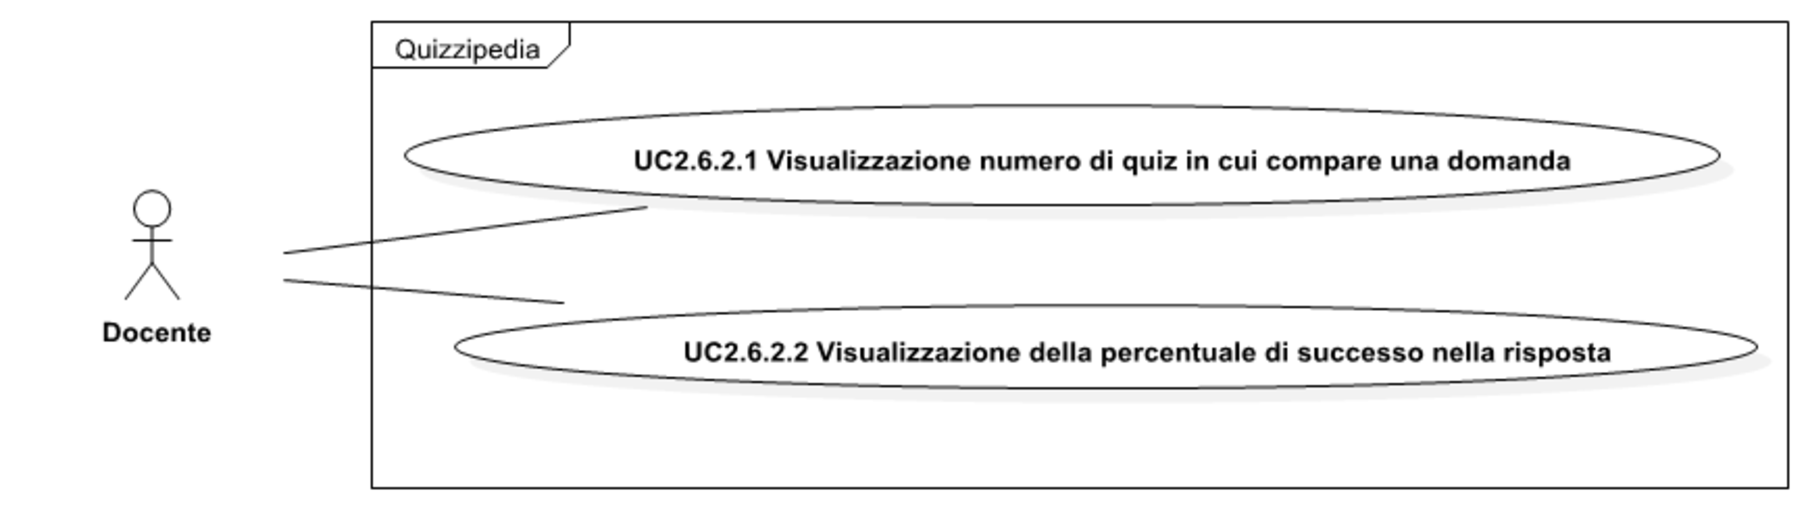
\includegraphics[width=\textwidth]{Img/UC Visualizzazione statistiche domande.pdf}}
\caption{UC2.7.2 Visualizzazione statistiche domande}
\end{figure}
\begin{itemize}
\item \textbf{Attori}: Docente.
\item \textbf{Scenario principale}:
\begin{enumerate}
\item Visualizzazione numero di quiz in cui compare una domanda (UC2.7.2.1);
\item Visualizzazione percentuale di successo nella risposta (UC2.7.2.2).
\end{enumerate}
\item \textbf{Descrizione}: il docente deve poter visualizzare statistiche legate alle domande.
\item \textbf{Precondizione}: il docente è autenticato nel sistema e desidera visualizzare le statistiche legate alle domande.
\item \textbf{Postcondizione}: il docente ha visualizzato le statistiche legate alle domande.
\end{itemize}
\subsubsection{UC2.7.2.1 Visualizzazione numero di quiz in cui compare una domanda}
\begin{itemize}
\item \textbf{Attori}: Docente.
\item \textbf{Scenario principale}: il docente visualizza il numero di quiz in cui compare la domanda.
\item \textbf{Descrizione}: il docente deve poter visualizzare il numero di quiz in cui compare la domanda.
\item \textbf{Precondizione}: il docente ha deciso di visualizzare le statistiche legate alle domande.
\item \textbf{Postcondizione}: il docente ha visualizzato il numero di quiz in cui compare una domanda.
\end{itemize}
\subsubsection{UC2.7.2.2 Visualizzazione percentuale di successo nella risposta}
\begin{itemize}
\item \textbf{Attori}: Docente.
\item \textbf{Scenario principale}: il docente visualizza la percentuale di successo nella risposta della domanda.
\item \textbf{Descrizione}: il docente deve poter visualizzare la percentuale di successo nella risposta della domanda.
\item \textbf{Precondizione}: il docente ha deciso di visualizzare le statistiche legate alle domande.
\item \textbf{Postcondizione}: il docente ha visualizzato la percentuale di successo nella risposta a una domanda.
\end{itemize}
\subsubsection{UC2.7.3 Visualizzazione statistiche studenti}
\begin{figure}[H]
\centering
\noindent\makebox[\textwidth]{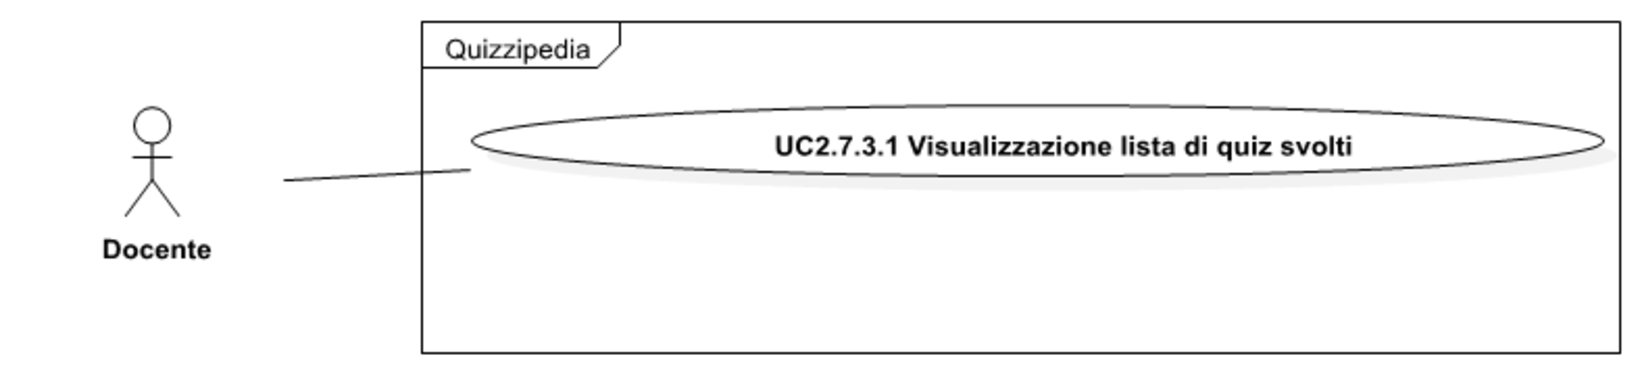
\includegraphics[width=\textwidth]{Img/UC Visualizzazione statistiche studenti.pdf}}
\caption{UC2.7.3 Visualizzazione statistiche studenti}
\end{figure}
\begin{itemize}
\item \textbf{Attori}: Docente.
\item \textbf{Scenario principale}:
\begin{enumerate}
\item Visualizzazione lista di quiz svolti (UC2.7.3.1).
\end{enumerate}
\item \textbf{Descrizione}:  il docente deve poter visualizzare statistiche legate agli studenti.
\item \textbf{Precondizione}: il docente è autenticato nel sistema e desidera visualizzare le statistiche legate agli studenti.
\item \textbf{Postcondizione}: il docente ha visualizzato le statistiche legate agli studenti.
\end{itemize}
\subsubsection{UC2.7.3.1 Visualizzazione lista di quiz svolti}
\begin{itemize}
\item \textbf{Attori}: Docente.
\item \textbf{Scenario principale}: il docente visualizza una lista dei quiz svolti dallo studente con rispettivo risultato.
\item \textbf{Descrizione}: il docente deve poter visualizzare una lista dei quiz svolti dallo studente con rispettivo risultato.
\item \textbf{Precondizione}: il docente ha deciso di visualizzare le statistiche legate agli studenti.
\item \textbf{Postcondizione}: il docente ha visualizzato la lista dei quiz svolti da uno studente.
\end{itemize}
\subsubsection{UC2.7.4 Visualizzazione statistiche docenti}
\begin{figure}[H]
\centering
\noindent\makebox[\textwidth]{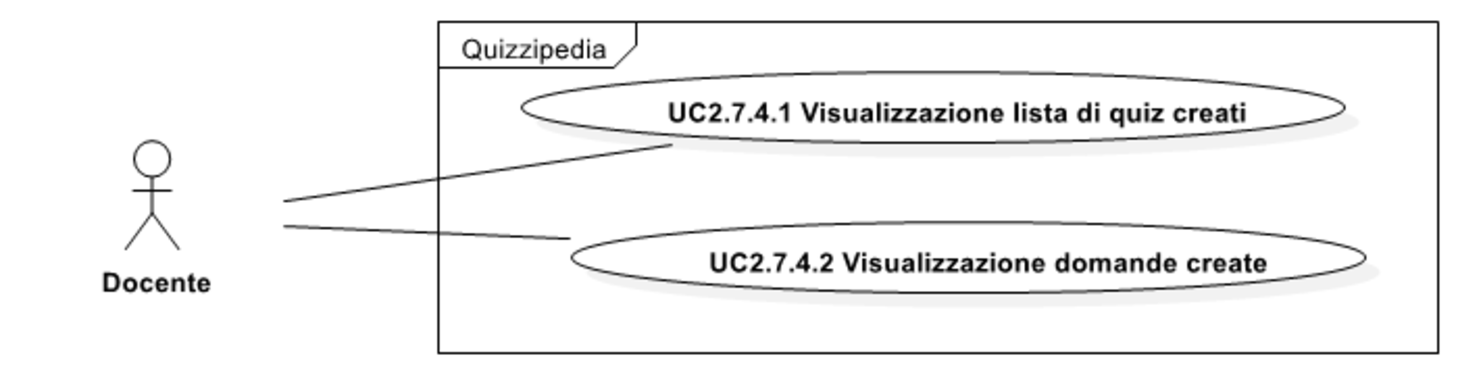
\includegraphics[width=\textwidth]{Img/UC Visualizzazione statistiche docenti.pdf}}
\caption{UC2.7.4 Visualizzazione statistiche docenti}
\end{figure}
\begin{itemize}
\item \textbf{Attori}: Docente.
\item \textbf{Scenario principale}:
\begin{enumerate}
\item Visualizzazione lista di quiz creati (UC2.7.4.1);
\item Visualizzazione lista di domande create (UC2.7.4.2).
\end{enumerate}
\item \textbf{Descrizione}: il docente deve poter visualizzare statistiche legate ai docenti.
\item \textbf{Precondizione}: il docente è autenticato nel sistema e desidera visualizzare le statistiche legate ai docenti.
\item \textbf{Postcondizione}: il docente ha visualizzato le statistiche legate ai docenti.
\end{itemize}
\subsubsection{UC2.7.4.1 Visualizzazione lista di quiz creati}
\begin{itemize}
\item \textbf{Attori}: Docente.
\item \textbf{Scenario principale}: il docente visualizza una lista dei quiz creati dal docente.
\item \textbf{Descrizione}: il docente deve poter visualizzare una lista dei quiz creati dal docente.
\item \textbf{Precondizione}: il docente ha deciso di visualizzare le statistiche legate ai docenti.
\item \textbf{Postcondizione}: il docente ha visualizzato la lista dei quiz creati da un docente.
\end{itemize}
\subsubsection{UC2.7.4.2 Visualizzazione lista di domande create}
\begin{itemize}
\item \textbf{Attori}: Docente.
\item \textbf{Scenario principale}: il docente visualizza una lista delle domande create dal docente.
\item \textbf{Descrizione}: il docente deve poter visualizzare una lista delle domande create dal docente.
\item \textbf{Precondizione}: il docente ha deciso di visualizzare le statistiche legate ai docenti.
\item \textbf{Postcondizione}: il docente ha visualizzato la lista delle domande create da un docente.
\end{itemize}
\subsubsection{UC2.8 Gestione enti}
\begin{figure}[H]
\centering
\noindent\makebox[\textwidth]{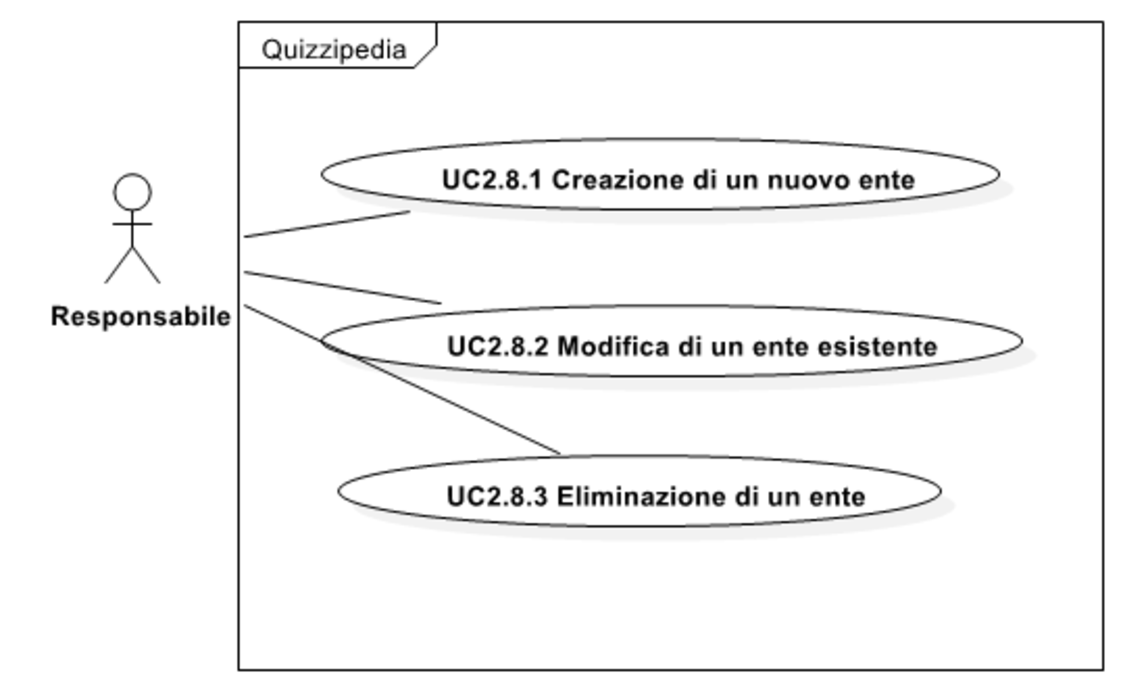
\includegraphics[width=\textwidth]{Img/UC Gestione enti.pdf}}
\caption{UC2.8 Gestione enti}
\end{figure}
\begin{itemize}
\item \textbf{Attori}: Responsabile.
\item \textbf{Scenario principale}:
\begin{enumerate}
\item Creazione di un nuovo ente (UC2.8.1);
\item Modifica di un ente esistente (UC2.8.2);
\item Eliminazione di un ente (UC2.8.3).
\end{enumerate}
\item \textbf{Descrizione}: il responsabile ha la completa gestione dell'ente di cui è a capo.
\item \textbf{Precondizione}: il responsabile ha il permesso di gestire l'ente.
\item \textbf{Postcondizione}: il responsabile ha completato la modifica delle informazioni desiderate riguardanti l'ente.
\end{itemize}
\subsubsection{UC2.8.1 Creazione di un nuovo ente}
\begin{figure}[H]
\centering
\noindent\makebox[\textwidth]{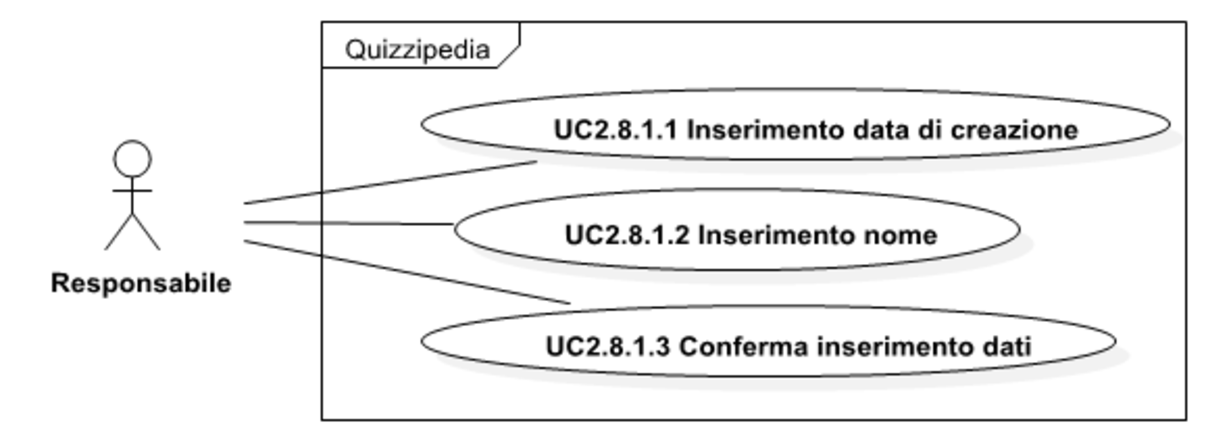
\includegraphics[width=\textwidth]{Img/UC Creazione di un nuovo ente.pdf}}
\caption{UC2.8.1 Creazione di un nuovo ente}
\end{figure}
\begin{itemize}
\item \textbf{Attori}: Responsabile.
\item \textbf{Scenario principale}:
\begin{enumerate}
\item Inserimento data di creazione (UC2.8.1.1);
\item Inserimento nome (UC2.8.1.2);
\item Conferma inserimento dati (UC2.8.1.3).
\end{enumerate}
\item \textbf{Descrizione}: il responsabile deve poter inserire un nuovo ente.
\item \textbf{Precondizione}: il responsabile ha il permesso di gestire l’ente.
\item \textbf{Postcondizione}: il responsabile ha creato un nuovo ente di cui ne è il capo.
\end{itemize}
\subsubsection{UC2.8.1.1 Inserimento data di creazione}
\begin{itemize}
\item \textbf{Attori}: Responsabile.
\item \textbf{Scenario principale}: il responsabile inserisce la data di creazione dell'ente.
\item \textbf{Descrizione}: il responsabile deve poter inserire la data di creazione dell'ente.
\item \textbf{Precondizione}: il responsabile sta creando l'ente.
\item \textbf{Postcondizione}: il responsabile ha inserito la data di creazione.
\end{itemize}
\subsubsection{UC2.8.1.2 Inserimento nome}
\begin{itemize}
\item \textbf{Attori}: Responsabile.
\item \textbf{Scenario principale}: il responsabile inserisce il nome dell'ente.
\item \textbf{Descrizione}:  il responsabile deve poter inserire il nome dell'ente.
\item \textbf{Precondizione}: il responsabile sta creando l'ente e deve ancora inserire il nome.
\item \textbf{Postcondizione}: il responsabile ha inserito il nome dell'ente.
\end{itemize}
\subsubsection{UC2.8.1.3 Conferma inserimento dati}
\begin{itemize}
\item \textbf{Attori}: Responsabile.
\item \textbf{Scenario principale}: il responsabile conferma i dati per la creazione dell'ente.
\item \textbf{Descrizione}: il responsabile conferma i dati precedentemente inseriti per avviare la creazione dell'ente.
\item \textbf{Precondizione}: il responsabile sta creando l'ente e deve ancora confermare i dati inseriti.
\item \textbf{Postcondizione}: i dati precedentemente inseriti sono stati confermati e l'ente è stato creato.
\end{itemize}
\subsubsection{UC2.8.2 Modifica di un ente esistente}
\begin{figure}[H]
\centering
\noindent\makebox[\textwidth]{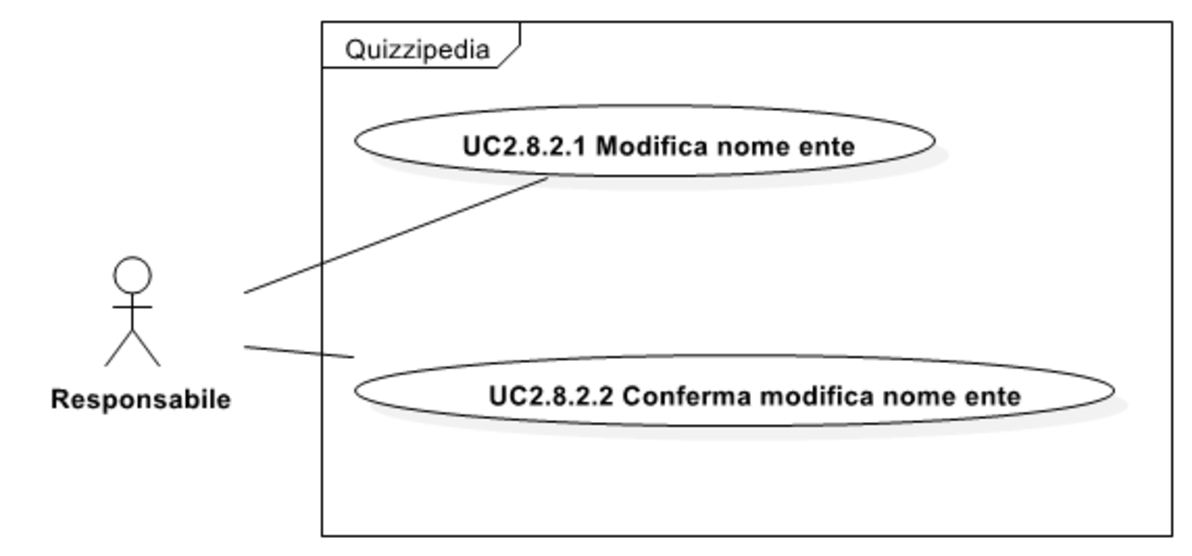
\includegraphics[width=\textwidth]{Img/UC Modifica di un ente esistente.pdf}}
\caption{UC2.8.2 Modifica di un ente esistente}
\end{figure}
\begin{itemize}
\item \textbf{Attori}: Responsabile.
\item \textbf{Scenario principale}:
\begin{enumerate}
\item Modifica nome ente (UC2.8.2.1);
\item Conferma modifica ente (UC2.8.2.2).
\end{enumerate}
\item \textbf{Descrizione}: il responsabile deve poter modificare i dati dell’ente che ha precedentemente creato.
\item \textbf{Precondizione}: il responsabile ha il permesso di modificare le informazioni dell’ente.
\item \textbf{Postcondizione}: il responsabile ha modificato le informazioni dell’ente.
\end{itemize}
\subsubsection{UC2.8.2.1 Modifica nome ente}
\begin{itemize}
\item \textbf{Attori}: Responsabile.
\item \textbf{Scenario principale}: il responsabile modifica il nome dell'ente.
\item \textbf{Descrizione}: il responsabile deve poter modificare il nome dell'ente.
\item \textbf{Precondizione}: il responsabile sta modificando i dati dell'ente e vuole modificare il nome.
\item \textbf{Postcondizione}: il responsabile ha modificato il nome dell'ente.
\end{itemize}
\subsubsection{UC2.8.2.2 Conferma modifica ente}
\begin{itemize}
\item \textbf{Attori}: Responsabile.
\item \textbf{Scenario principale}: il responsabile conferma la modifica dell'ente.
\item \textbf{Descrizione}: il responsabile deve confermare la modifica dell'ente.
\item \textbf{Precondizione}: il responsabile ha modificando i dati dell'ente e deve ancora confermare le modifiche fatte.
\item \textbf{Postcondizione}: il responsabile ha confermato le modifiche effettuate.
\end{itemize}
\subsubsection{UC2.8.3 Eliminazione di un ente}
\begin{figure}[H]
\centering
\noindent\makebox[\textwidth]{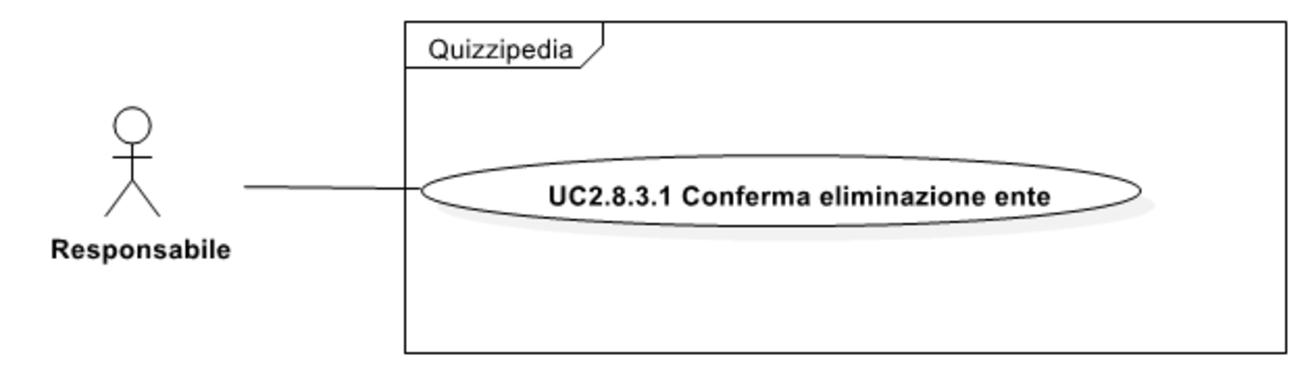
\includegraphics[width=\textwidth]{Img/UC Eliminazione di un ente.pdf}}
\caption{UC2.8.3 Eliminazione di un ente}
\end{figure}
\begin{itemize}
\item \textbf{Attori}: Responsabile.
\item \textbf{Scenario principale}:
\begin{enumerate}
\item Conferma eliminazione ente (UC2.8.3.1).
\end{enumerate}
\item \textbf{Descrizione}: il responsabile deve poter eliminare un ente di cui è proprietario.
\item \textbf{Precondizione}: il responsabile è nella gestione degli enti e vuole eliminare un suo ente.
\item \textbf{Postcondizione}: il responsabile ha eliminato l’ente.
\end{itemize}
\subsubsection{UC2.8.3.1 Conferma eliminazione ente}
\begin{itemize}
\item \textbf{Attori}: Responsabile.
\item \textbf{Scenario principale}: il responsabile conferma l'eliminazione dell'ente.
\item \textbf{Descrizione}: il responsabile deve confermare l'eliminazione dell'ente.
\item \textbf{Precondizione}: il responsabile ha scelto un ente da eliminare e deve ancora confermare.
\item \textbf{Postcondizione}: il responsabile ha confermato l'ente da eliminare.
\end{itemize}
\subsubsection{UC2.9 Gestione classe}
\begin{figure}[H]
\centering
\noindent\makebox[\textwidth]{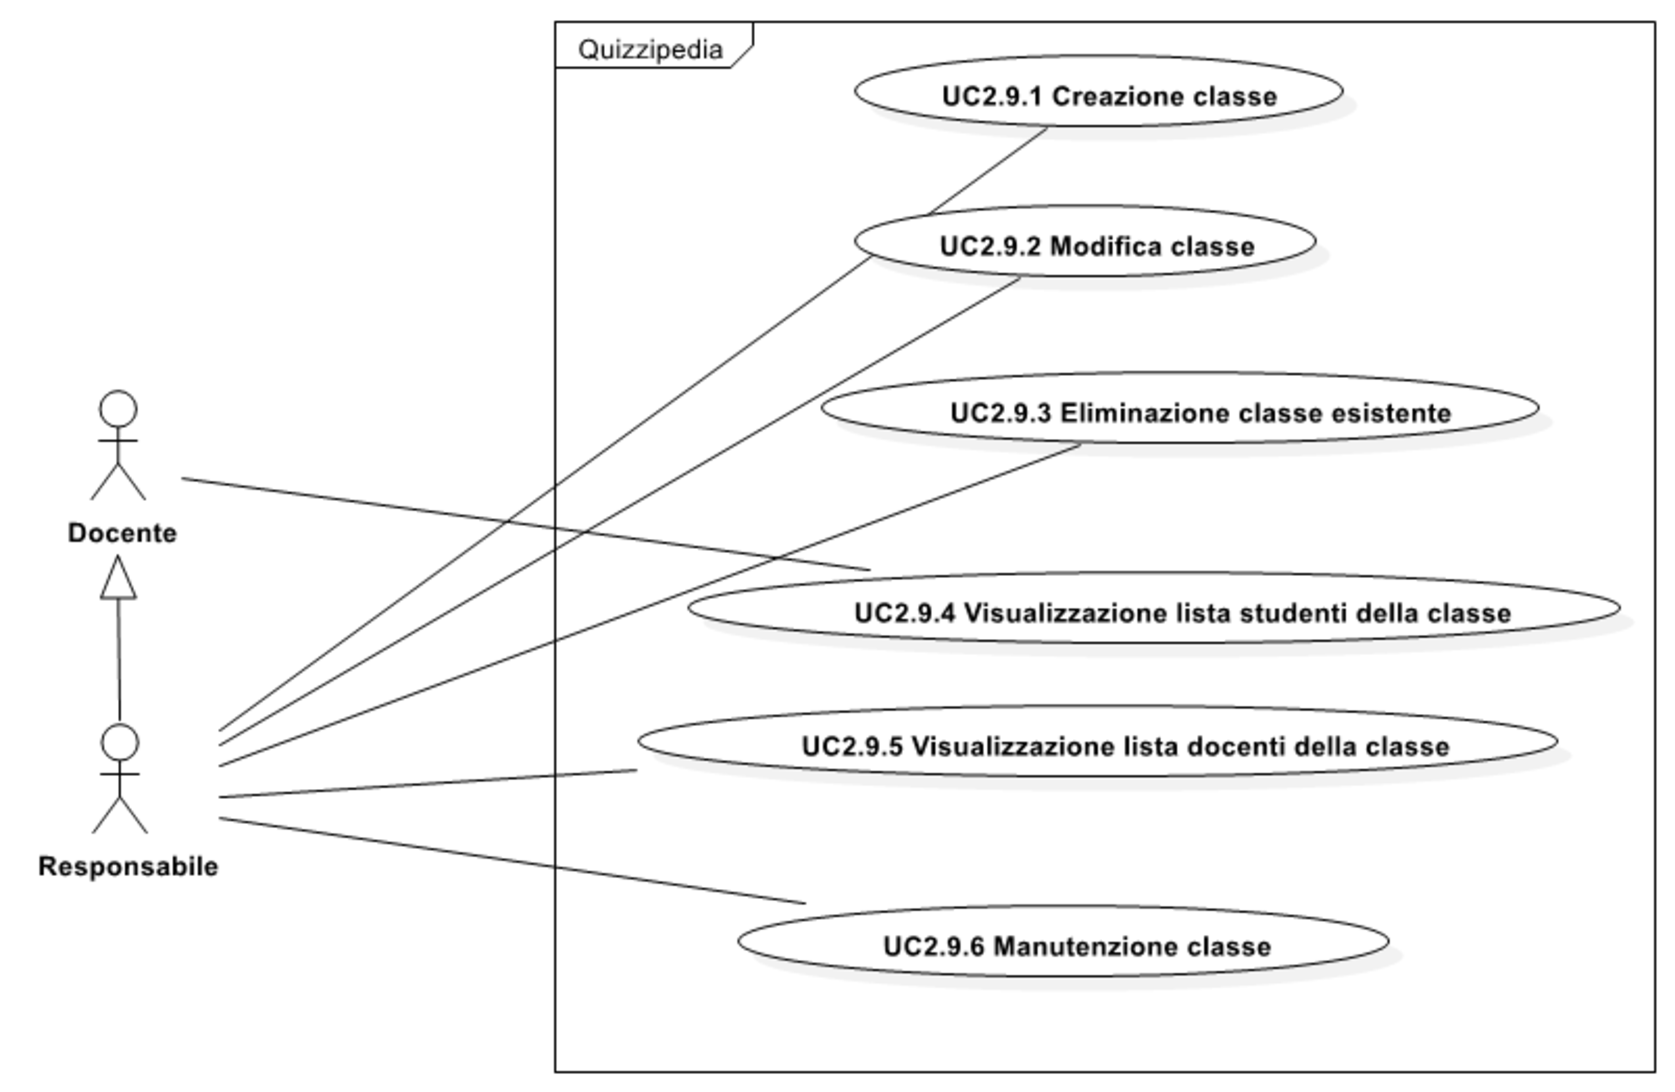
\includegraphics[width=\textwidth]{Img/UC Gestione classe.pdf}}
\caption{UC2.9 Gestione classe}
\end{figure}
\begin{itemize}
\item \textbf{Attori}: Responsabile.
\item \textbf{Scenario principale}:
\begin{enumerate}
\item Creazione classe (UC2.9.1);
\item Modifica classe (UC2.9.2);
\item Eliminazione classe esistente (UC2.9.3);
\item Visualizza lista studenti della classe (UC2.9.4);
\item Visualizza lista docenti della classe (UC2.9.5);
\item Manutenzione classe (UC2.9.6).
\end{enumerate}
\item \textbf{Descrizione}: il responsabile può creare, modificare ed eliminare una classe; inoltre può visualizzare la lista degli studenti e docenti della classe; può fare manutenzione sulle classi nel caso in cui le richieste di inserimento da parte di studenti e docenti siano sbagliate; infine gestisce la lista delle richieste che riceve da parte degli studenti e docenti.
\item \textbf{Precondizione}: il responsabile ha i permessi per gestire le classi.
\item \textbf{Postcondizione}: il responsabile ha effettuato le operazioni di gestione delle classi.
\end{itemize}
\subsubsection{UC2.9.1 Creazione classe}
\begin{figure}[H]
\centering
\noindent\makebox[\textwidth]{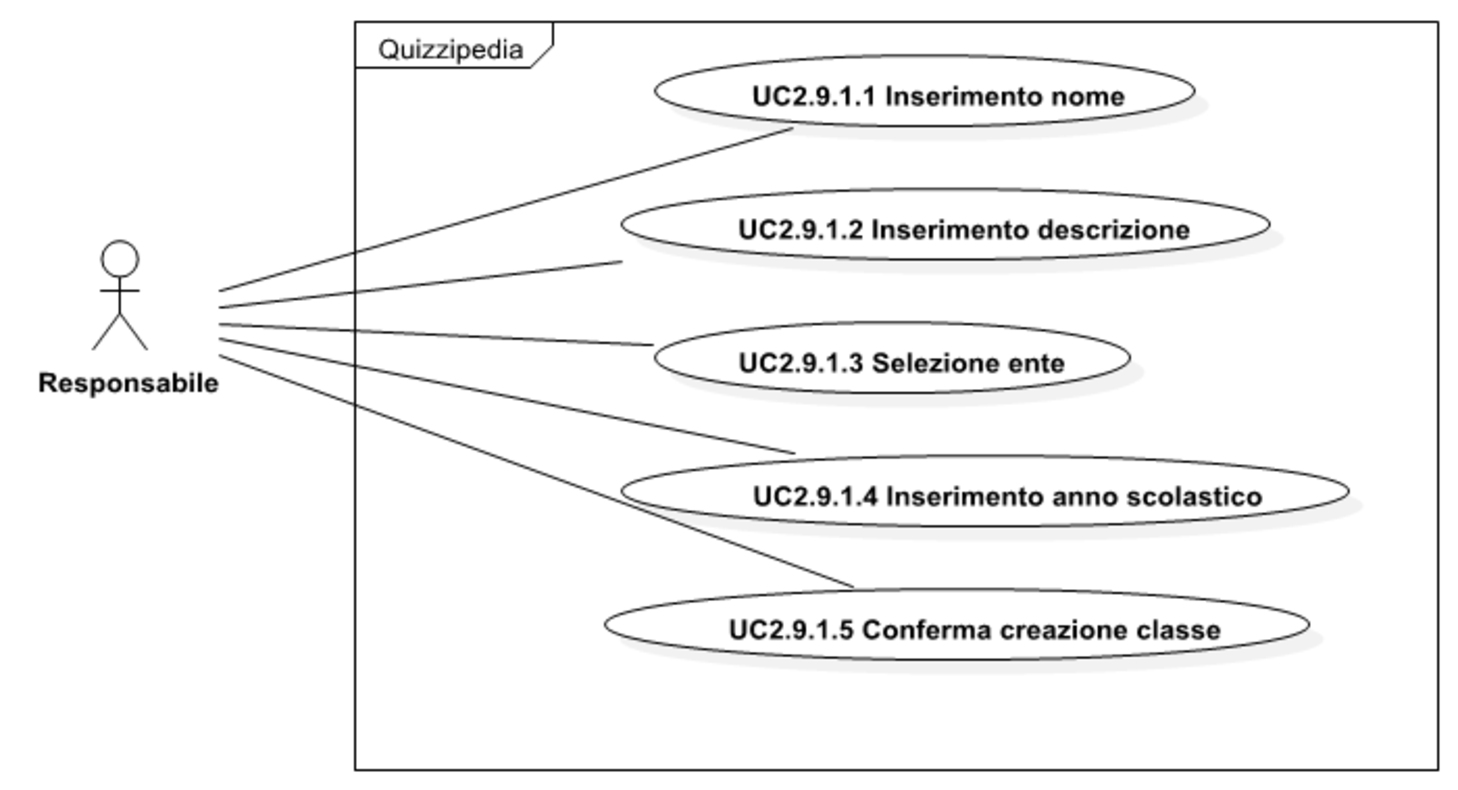
\includegraphics[width=\textwidth]{Img/UC Creazione classe.pdf}}
\caption{UC2.9.1 Creazione classe}
\end{figure}
\begin{itemize}
\item \textbf{Attori}: Responsabile.
\item \textbf{Scenario principale}:
\begin{enumerate}
\item Inserimento nome (UC2.9.1.1);
\item Inserimento descrizione (UC2.9.1.2);
\item Selezione ente (UC2.9.1.3);
\item Inserimento anno scolastico (UC2.9.1.4);
\item Conferma creazione classe (UC2.9.1.5).
\end{enumerate}
\item \textbf{Descrizione}: il responsabile deve poter creare una classe.
\item \textbf{Precondizione}: il responsabile ha i permessi per creare una classe ed è nella gestione classe.
\item \textbf{Postcondizione}: il responsabile ha creato una nuova classe.
\end{itemize}
\subsubsection{UC2.9.1.1 Inserimento nome}
\begin{itemize}
\item \textbf{Attori}: Responsabile.
\item \textbf{Scenario principale}: il responsabile inserisce il nome della classe.
\item \textbf{Descrizione}: il responsabile deve poter inserire il nome della classe.
\item \textbf{Precondizione}: il responsabile sta creando una classe e deve ancora inserire il nome.
\item \textbf{Postcondizione}: il responsabile ha inserito il nome della classe.
\end{itemize}
\subsubsection{UC2.9.1.2 Inserimento descrizione}
\begin{itemize}
\item \textbf{Attori}: Responsabile.
\item \textbf{Scenario principale}: il responsabile inserisce la descrizione della classe.
\item \textbf{Descrizione}: il responsabile può inserire una breve descrizione della classe.
\item \textbf{Precondizione}: il responsabile sta creando una classe e deve ancora inserire la descrizione.
\item \textbf{Postcondizione}: il responsabile ha inserito una breve descrizione della classe.
\end{itemize}
\subsubsection{UC2.9.1.3 Selezione ente}
\begin{itemize}
\item \textbf{Attori}: Responsabile.
\item \textbf{Scenario principale}: il responsabile seleziona l'ente proprietario della classe.
\item \textbf{Descrizione}: il responsabile deve selezionare l'ente che sarà il proprietario della classe.
\item \textbf{Precondizione}: il responsabile sta creando una classe e deve ancora selezionare l'ente.
\item \textbf{Postcondizione}: il responsabile ha selezionato l'ente proprietario della classe.
\end{itemize}
\subsubsection{UC2.9.1.4 Inserimento anno scolastico}
\begin{itemize}
\item \textbf{Attori}: Responsabile.
\item \textbf{Scenario principale}: il responsabile inserisce l'anno scolastico di creazione della classe.
\item \textbf{Descrizione}: il responsabile deve inserire l'anno scolastico in cui è stata creata la classe.
\item \textbf{Precondizione}: il responsabile sta creando una classe e deve ancora inserire l'anno scolastico.
\item \textbf{Postcondizione}: il responsabile ha inserito l'anno scolastico della classe.
\end{itemize}
\subsubsection{UC2.9.1.5 Conferma creazione classe}
\begin{itemize}
\item \textbf{Attori}: Responsabile.
\item \textbf{Scenario principale}: il responsabile conferma i dati per la creazione della classe.
\item \textbf{Descrizione}: il responsabile deve confermare i dati precedentemente inseriti.
\item \textbf{Precondizione}: il responsabile ha inserito una nuova classe e deve ancora confermarla.
\item \textbf{Postcondizione}: il responsabile ha confermato i dati inseriti e la classe è stata creata.
\end{itemize}
\subsubsection{UC2.9.2 Modifica classe}
\begin{figure}[H]
\centering
\noindent\makebox[\textwidth]{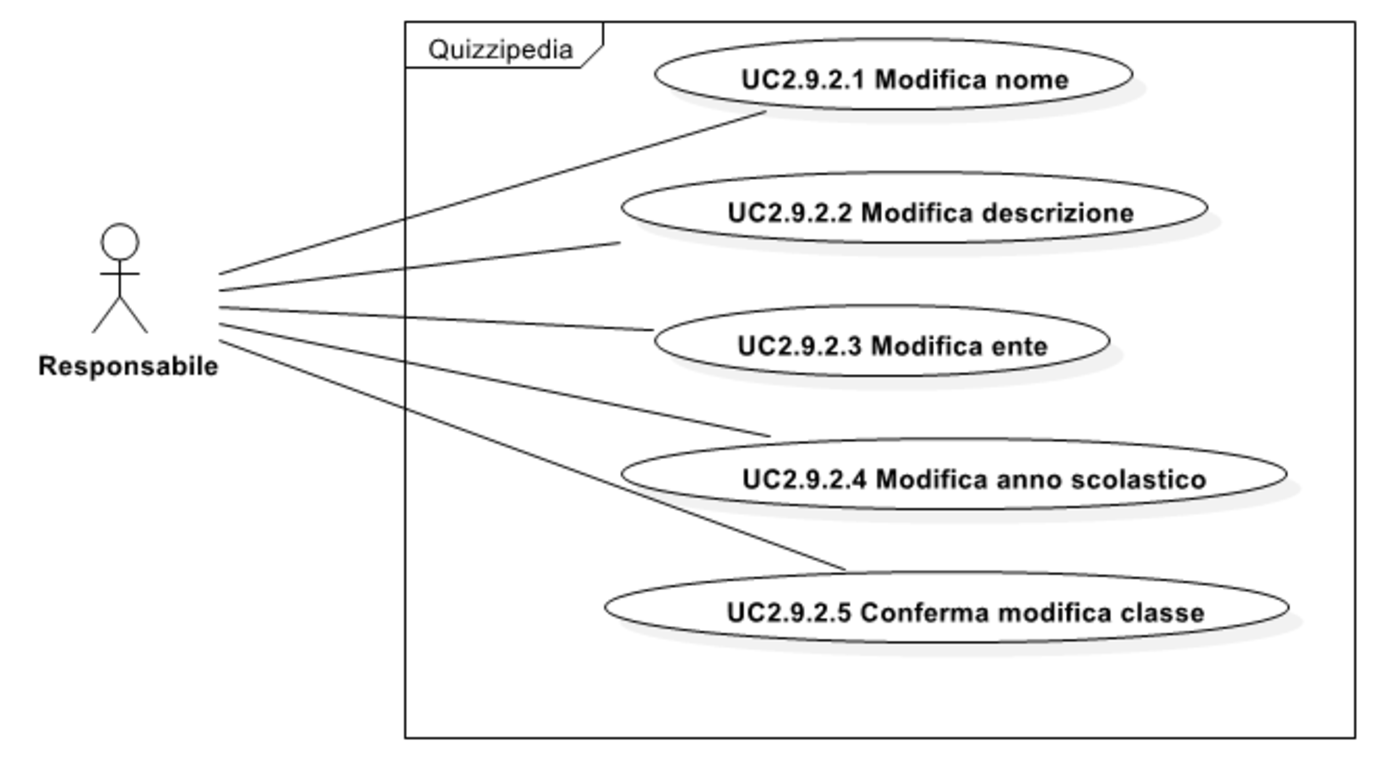
\includegraphics[width=\textwidth]{Img/UC Modifica classe.pdf}}
\caption{UC2.9.2 Modifica classe}
\end{figure}
\begin{itemize}
\item \textbf{Attori}: Responsabile.
\item \textbf{Scenario principale}:
\begin{enumerate}
\item Modifica nome (UC2.9.2.1);
\item Modifica descrizione (UC2.9.2.2);
\item Modifica ente (UC2.9.2.3);
\item Modifica anno scolastico (UC2.9.2.4);
\item Conferma modifica classe (UC2.9.2.5).
\end{enumerate}
\item \textbf{Descrizione}: il responsabile deve poter modificare i dati della classe.
\item \textbf{Precondizione}: il responsabile ha i permessi per modificare una classe.
\item \textbf{Postcondizione}: il responsabile ha effettuato le modifiche sulla classe.
\end{itemize}
\subsubsection{UC2.9.2.1 Modifica nome}
\begin{itemize}
\item \textbf{Attori}: Responsabile.
\item \textbf{Scenario principale}: il responsabile modifica il nome della classe.
\item \textbf{Descrizione}: il responsabile deve poter modificare il nome della classe.
\item \textbf{Precondizione}: il responsabile sta modificando la classe.
\item \textbf{Postcondizione}: il responsabile ha modificato il nome della classe.
\end{itemize}
\subsubsection{UC2.9.2.2 Modifica descrizione}
\begin{itemize}
\item \textbf{Attori}: Responsabile.
\item \textbf{Scenario principale}: il responsabile modifica la descrizione della classe.
\item \textbf{Descrizione}: il responsabile deve poter modificare la descrizione della classe.
\item \textbf{Precondizione}: il responsabile sta modificando la classe.
\item \textbf{Postcondizione}: il responsabile ha modificato la descrizione della classe.
\end{itemize}
\subsubsection{UC2.9.2.3 Modifica ente}
\begin{itemize}
\item \textbf{Attori}: Responsabile.
\item \textbf{Scenario principale}: il responsabile modifica l'ente della classe.
\item \textbf{Descrizione}: il responsabile deve poter modificare l'ente della classe a cui è associata.
\item \textbf{Precondizione}: il responsabile sta modificando la classe.
\item \textbf{Postcondizione}: il responsabile ha modificato l'ente della classe.
\end{itemize}
\subsubsection{UC2.9.2.4 Modifica anno scolastico}
\begin{itemize}
\item \textbf{Attori}: Responsabile.
\item \textbf{Scenario principale}: il responsabile modifica l'anno scolastico di creazione della classe.
\item \textbf{Descrizione}: il responsabile deve poter modificare l'anno scolastico della creazione della classe.
\item \textbf{Precondizione}: il responsabile sta modificando la classe.
\item \textbf{Postcondizione}: il responsabile ha modificato l'anno scolastico della classe.
\end{itemize}
\subsubsection{UC2.9.2.5 Conferma modifica classe}
\begin{itemize}
\item \textbf{Attori}: Responsabile.
\item \textbf{Scenario principale}: il responsabile conferma la modifica della classe.
\item \textbf{Descrizione}: il responsabile deve confermare le modifiche precedentemente fatte.
\item \textbf{Precondizione}: il responsabile ha modificato la classe e deve ancora confermare le modifiche.
\item \textbf{Postcondizione}: il responsabile ha confermato le modifiche.
\end{itemize}
\subsubsection{UC2.9.3 Eliminazione classe esistente}
\begin{figure}[H]
\centering
\noindent\makebox[\textwidth]{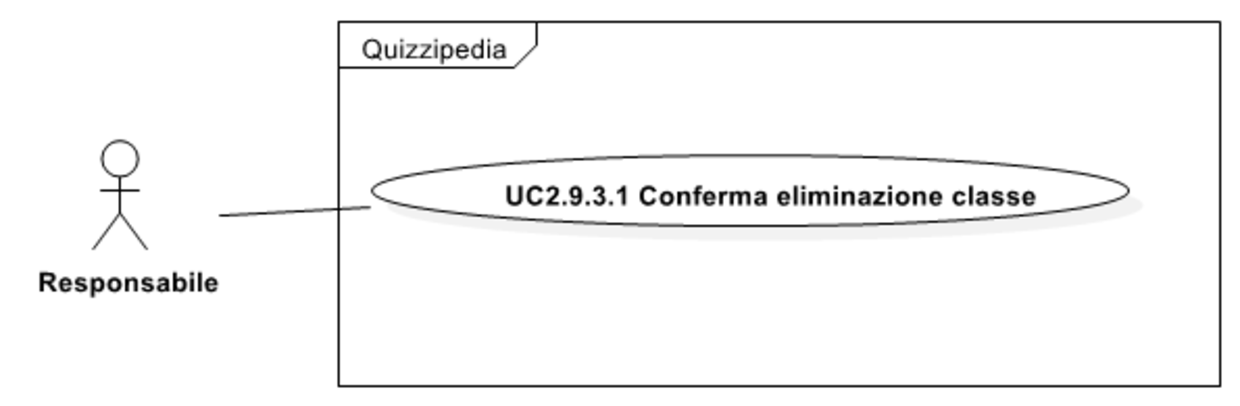
\includegraphics[width=\textwidth]{Img/UC Eliminazione classe esistente.pdf}}
\caption{UC2.9.3 Eliminazione classe esistente}
\end{figure}
\begin{itemize}
\item \textbf{Attori}: Responsabile.
\item \textbf{Scenario principale}:
\begin{enumerate}
\item Conferma eliminazione classe (UC2.9.3.1).
\end{enumerate}
\item \textbf{Descrizione}: il responsabile può eliminare una classe.
\item \textbf{Precondizione}: il responsabile ha i permessi per eliminare una classe.
\item \textbf{Postcondizione}: il responsabile ha eliminato la classe.
\end{itemize}
\subsubsection{UC2.9.3.1 Conferma eliminazione classe}
\begin{itemize}
\item \textbf{Attori}: Responsabile.
\item \textbf{Scenario principale}: il responsabile conferma l'eliminazione della classe.
\item \textbf{Descrizione}: il responsabile deve confermare l'eliminazione della classe.
\item \textbf{Precondizione}: il responsabile vuole eliminare una classe e deve ancora confermare.
\item \textbf{Postcondizione}: il responsabile ha confermato l'eliminazione della classe.
\end{itemize}
\subsubsection{UC2.9.4 Visualizza lista studenti della classe}
\begin{itemize}
\item \textbf{Attori}: Docente.
\item \textbf{Scenario principale}: il docente visualizza la lista degli studenti di una classe.
\item \textbf{Descrizione}: il docente seleziona il nome della classe e può visualizzare la lista di studenti associati a quella classe.
\item \textbf{Precondizione}: il responsabile e il docente hanno il permesso di consultare la lista degli studenti.
\item \textbf{Postcondizione}: vengono visualizzati gli studenti della classe selezionata.
\end{itemize}
\subsubsection{UC2.9.5 Visualizza lista docenti della classe}
\begin{itemize}
\item \textbf{Attori}: Responsabile.
\item \textbf{Scenario principale}: il responsabile visualizza la lista di docenti di una classe.
\item \textbf{Descrizione}: il responsabile seleziona il nome della classe e può visualizzare la lista di docenti associati a quella classe.
\item \textbf{Precondizione}: il responsabile ha il permesso di consultare la lista dei docenti.
\item \textbf{Postcondizione}: il responsabile visualizza i docenti della classe selezionata.
\end{itemize}
\subsubsection{UC2.9.6 Manutenzione classe}
\begin{figure}[H]
\centering
\noindent\makebox[\textwidth]{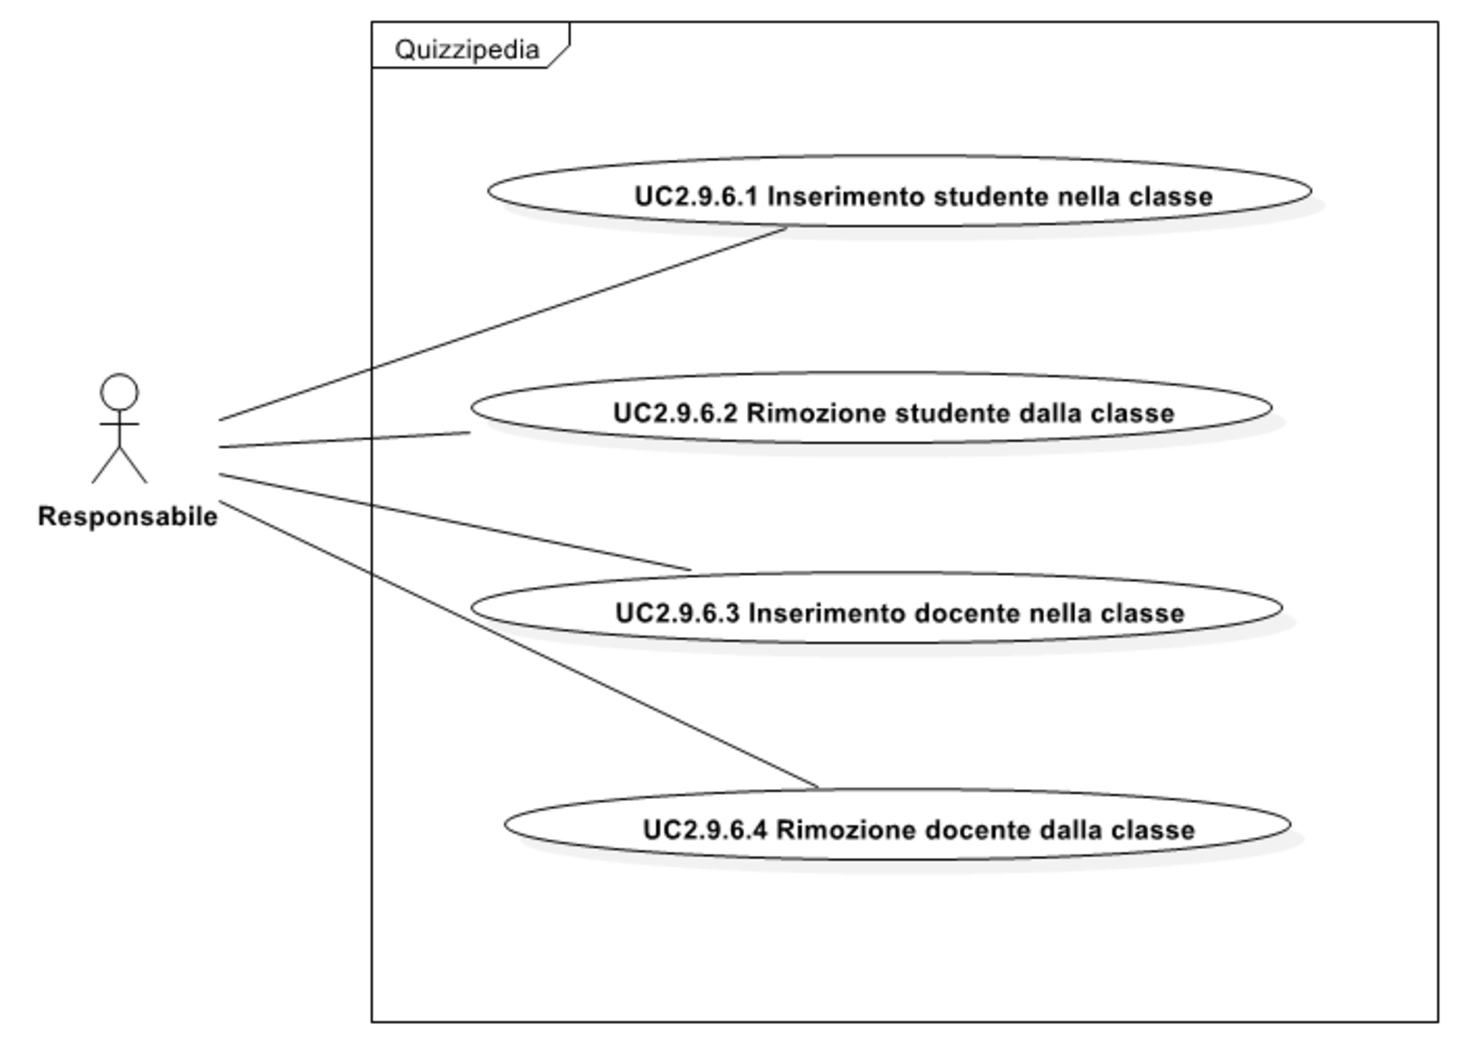
\includegraphics[width=\textwidth]{Img/UC Manutenzione classe.pdf}}
\caption{UC2.9.6 Manutenzione classe}
\end{figure}
\begin{itemize}
\item \textbf{Attori}: Responsabile.
\item \textbf{Scenario principale}:
\begin{enumerate}
\item Inserimento studente nella classe (UC2.9.6.1);
\item Rimozione studente dalla classe (UC2.9.6.2);
\item Inserimento docente nella classe (UC2.9.6.3);
\item Rimozione docente dalla classe (UC2.9.6.4).
\end{enumerate}
\item \textbf{Descrizione}: il responsabile può fare manutenzione su una classe nel caso in cui uno studente o un docente si sia inscritto in una classe sbagliata. Il responsabile procederà alla rimozione con successivo inserimento dello studente o del docente nella classe corretta.
\item \textbf{Precondizione}: il responsabile ha il permesso di fare manutenzione alla classe.
\item \textbf{Postcondizione}: il responsabile ha fatto alcune operazioni di manutenzione alla classe.
\end{itemize}
\subsubsection{UC2.9.6.1 Inserimento studente nella classe}
\begin{itemize}
\item \textbf{Attori}: Responsabile.
\item \textbf{Scenario principale}: il responsabile inserisce uno studente nella classe.
\item \textbf{Descrizione}: il responsabile può inserire uno studente nella classe.
\item \textbf{Precondizione}: il responsabile ha deciso di effettuare la manutenzione della classe.
\item \textbf{Postcondizione}: il responsabile ha inserito lo studente nella classe.
\end{itemize}
\subsubsection{UC2.9.6.2 Rimozione studente dalla classe}
\begin{itemize}
\item \textbf{Attori}: Responsabile.
\item \textbf{Scenario principale}: il responsabile rimuove uno studente dalla classe.
\item \textbf{Descrizione}: il responsabile può rimuovere uno studente dalla classe.
\item \textbf{Precondizione}: il responsabile ha deciso di effettuare la manutenzione della classe.
\item \textbf{Postcondizione}: il responsabile ha rimosso lo studente dalla classe.
\end{itemize}
\subsubsection{UC2.9.6.3 Inserimento docente nella classe}
\begin{itemize}
\item \textbf{Attori}: Responsabile.
\item \textbf{Scenario principale}: il responsabile inserisce un docente nella classe.
\item \textbf{Descrizione}: il responsabile può inserire un docente nella classe.
\item \textbf{Precondizione}: il responsabile ha deciso di effettuare la manutenzione della classe.
\item \textbf{Postcondizione}: il responsabile ha inserito il docente nella classe.
\end{itemize}
\subsubsection{UC2.9.6.4 Rimozione docente dalla classe}
\begin{itemize}
\item \textbf{Attori}: Responsabile.
\item \textbf{Scenario principale}: il responsabile rimuove un docente dalla classe.
\item \textbf{Descrizione}: il responsabile può rimuovere un docente dalla classe.
\item \textbf{Precondizione}: il responsabile ha deciso di effettuare la modifica della classe.
\item \textbf{Postcondizione}: il responsabile ha rimosso il docente dalla classe.
\end{itemize}
\subsubsection{UC2.10 Lista richieste}
\begin{figure}[H]
\centering
\noindent\makebox[\textwidth]{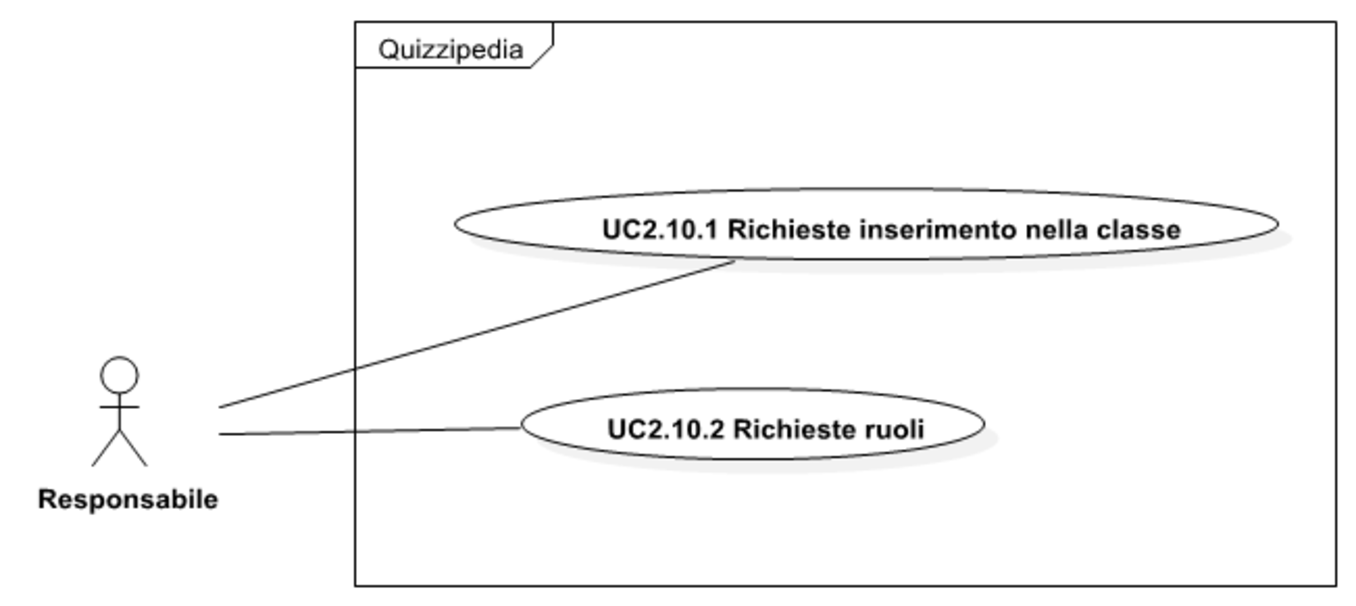
\includegraphics[width=\textwidth]{Img/UC Lista richieste.pdf}}
\caption{UC2.10 Lista richieste}
\end{figure}
\begin{itemize}
\item \textbf{Attori}: Responsabile.
\item \textbf{Scenario principale}:
\begin{enumerate}
\item Richieste inserimento nella classe (UC2.10.1);
\item Richieste ruoli (UC2.10.2).
\end{enumerate}
\item \textbf{Descrizione}: il responsabile gestisce le richieste inviate da studenti, docenti ed utenti senza ruolo per accettare o annullare il ruolo richiesto o per accettare e annullare l’inserimento dello studente o docente in una determinata classe.
\item \textbf{Precondizione}: il responsabile ha i permessi per la gestione delle richieste.
\item \textbf{Postcondizione}: il responsabile ha accettato o rifiutato alcune richieste che ha ricevuto.
\end{itemize}
\subsubsection{UC2.10.1 Richieste inserimento nella classe}
\begin{figure}[H]
\centering
\noindent\makebox[\textwidth]{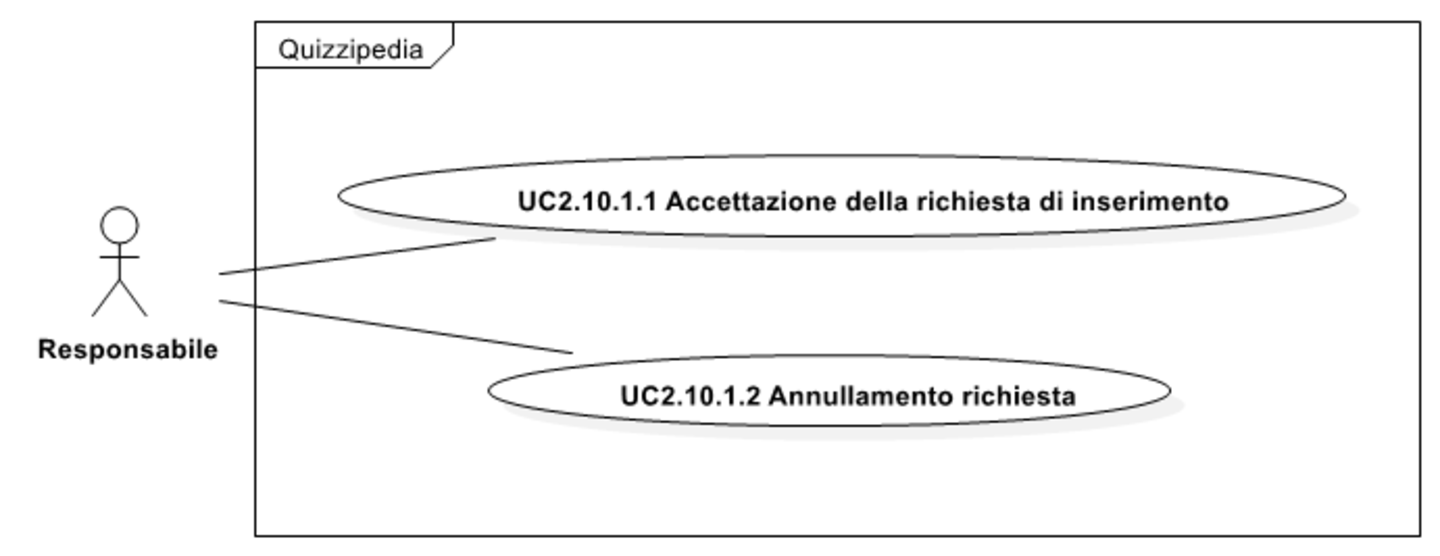
\includegraphics[width=\textwidth]{Img/UC Richieste inserimento nella classe.pdf}}
\caption{UC2.10.1 Richieste inserimento nella classe}
\end{figure}
\begin{itemize}
\item \textbf{Attori}: Responsabile.
\item \textbf{Scenario principale}:
\begin{enumerate}
\item Accettazione della richiesta di inserimento (UC2.10.1.1);
\item Annullamento della richiesta di inserimento (UC2.10.1.2).
\end{enumerate}
\item \textbf{Descrizione}: il responsabile accetta o rifiuta le richieste di inserimento nella classe ricevute dagli studenti e docenti.
\item \textbf{Precondizione}: il responsabile visualizza la lista di richieste di inserimento nella classe.
\item \textbf{Postcondizione}: il responsabile ha accettato o rifiutato le richieste che ha ricevuto.
\end{itemize}
\subsubsection{UC2.10.1.1 Accettazione della richiesta di inserimento}
\begin{itemize}
\item \textbf{Attori}: Responsabile.
\item \textbf{Scenario principale}: il responsabile accetta le richieste di inserimento nella classe.
\item \textbf{Descrizione}: il responsabile accetta le richieste di inserimento nella classe ricevute dagli studenti e docenti.
\item \textbf{Precondizione}: il responsabile visualizza lista richieste di inserimento nella classe.
\item \textbf{Postcondizione}: il responsabile ha accettato le richieste di inserimento nella classe che gli sono pervenute dagli studenti e docenti.
\end{itemize}
\subsubsection{UC2.10.1.2 Annullamento della richiesta di inserimento}
\begin{itemize}
\item \textbf{Attori}: Responsabile.
\item \textbf{Scenario principale}: il responsabile rifiuta le richieste di inserimento nella classe.
\item \textbf{Descrizione}: il responsabile rifiuta le richieste di inserimento nella classe ricevute dagli studenti e docenti.
\item \textbf{Precondizione}: il responsabile visualizza lista richieste di inserimento nella classe.
\item \textbf{Postcondizione}: il responsabile ha rifiutato le richieste di inserimento nella classe che gli sono pervenute dagli studenti e docenti.
\end{itemize}
\subsubsection{UC2.10.2 Richieste ruoli}
\begin{figure}[H]
\centering
\noindent\makebox[\textwidth]{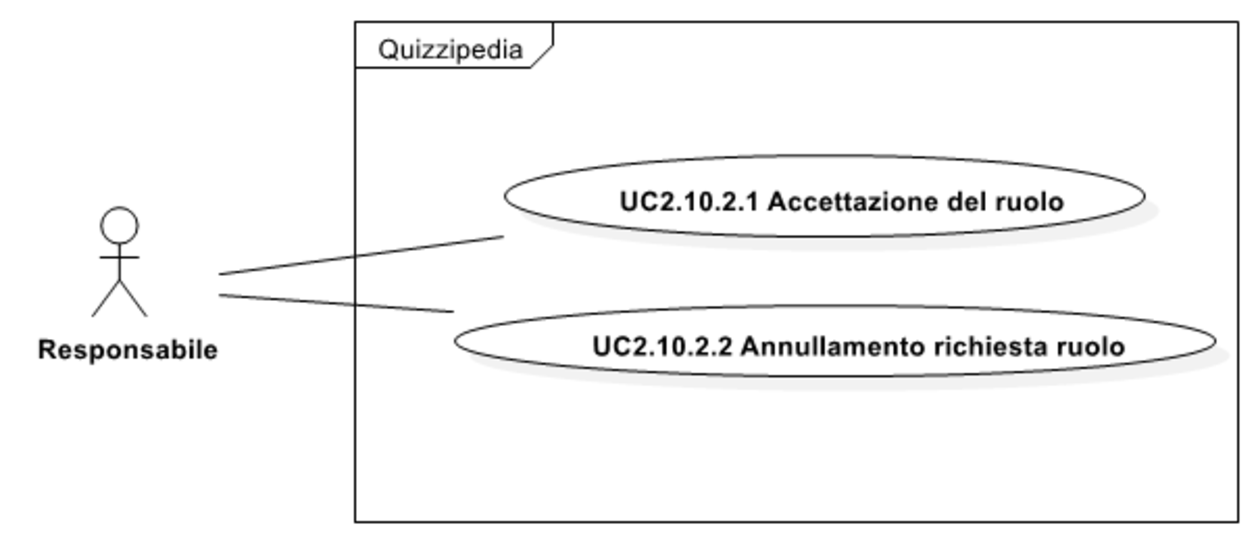
\includegraphics[width=\textwidth]{Img/UC Richieste ruoli.pdf}}
\caption{UC2.10.2 Richieste ruoli}
\end{figure}
\begin{itemize}
\item \textbf{Attori}: Responsabile.
\item \textbf{Scenario principale}:
\begin{enumerate}
\item Accettazione del ruolo (UC2.10.2.1);
\item Annullamento richiesta ruolo (UC2.10.2.2).
\end{enumerate}
\item \textbf{Descrizione}: il responsabile accetta o rifiuta le richieste  del ruolo che vogliono assumere gli utenti senza ruolo.
\item \textbf{Precondizione}: il responsabile ha i permessi per la gestione della lista richieste.
\item \textbf{Postcondizione}: il responsabile ha accettato o rifiutato le richieste dei ruoli che gli sono pervenute dagli utenti senza ruolo.
\end{itemize}
\subsubsection{UC2.10.2.1 Accettazione del ruolo}
\begin{itemize}
\item \textbf{Attori}: Responsabile.
\item \textbf{Scenario principale}: il responsabile accetta le richieste di ruolo.
\item \textbf{Descrizione}: il responsabile accetta  le richieste del ruolo che vogliono assumere gli utenti senza ruolo.
\item \textbf{Precondizione}: il responsabile visualizza la lista richieste ruoli.
\item \textbf{Postcondizione}: il responsabile ha accettato le richieste del ruolo che gli sono pervenute dagli utenti senza ruolo.
\end{itemize}
\subsubsection{UC2.10.2.2 Annullamento richiesta ruolo}
\begin{itemize}
\item \textbf{Attori}: Responsabile.
\item \textbf{Scenario principale}: il responsabile rifiuta le richieste di ruolo.
\item \textbf{Descrizione}: il responsabile rifiuta le richieste  del ruolo che vogliono assumere gli utenti senza ruolo.
\item \textbf{Precondizione}: il responsabile visualizza la lista richieste ruoli.
\item \textbf{Postcondizione}: il responsabile ha rifiutato le richieste del ruolo che gli sono pervenute dagli utenti senza ruolo.
\end{itemize}
\subsubsection{UC2.11 Gestione domande}
\begin{itemize}
\item \textbf{Attori}: Docente.
\item \textbf{Scenario principale}:
\begin{enumerate}
\item Creazione domanda (UC2.11.1);
\item Errore numero risposte creazione (UC2.11.2);
\item Interruzione volontaria della creazione della domanda (UC2.11.3);
\item Creazione domanda vero o falso (UC2.11.4);
\item Creazione domanda risposta multipla (UC2.11.5);
\item Creazione domanda a collegamenti (UC2.11.6);
\item Creazione domanda a risposta aperta (UC2.11.7);
\item UC Creazione domanda a completamento testo (UC2.11.8);
\item Modifica domanda (UC2.11.9);
\item Errore numero risposte modifica (UC2.11.10);
\item Interruzione volontaria della modifica della domanda (UC2.11.11);
\item Modifica domanda vero o falso (UC2.11.12);
\item Modifica domanda risposta multipla (UC2.11.13);
\item Modifica domanda a risposta aperta (UC2.11.14);
\item Modifica domanda a completamento testo (UC2.11.15);
\item Modifica domanda a collegamenti (UC2.11.16).
\end{enumerate}
\item \textbf{Descrizione}: il docente deve poter effettuare varie operazioni sulle domande, in particolare creare nuove domande di vario tipo e modificare o eliminare domande esistenti.
\item \textbf{Precondizione}: il sistema ha riconosciuto il docente e ora può gestire le domande.
\item \textbf{Postcondizione}: il docente ha completato le operazioni sulle domande con successo.
\end{itemize}
\subsubsection{UC2.11.1 Creazione domanda}
\begin{itemize}
\item \textbf{Attori}: Docente.
\item \textbf{Scenario principale}:
\begin{enumerate}
\item Inserimento titolo domanda (UC2.11.1.1);
\item Descrizione aggiuntiva (UC2.11.1.2);
\item Selezione argomento della domanda (UC2.11.1.3);
\item Selezione livello di difficoltà (UC2.11.1.4);
\item Inserire allegato (UC2.11.1.5).
\end{enumerate}
\item \textbf{Estensioni}:
\begin{itemize}
\item Errore numero risposte creazione (UC2.11.2);
\item Interruzione volontaria della creazione della domanda (UC2.11.3).
\end{itemize}
\item \textbf{Generalizzazioni}:
\begin{itemize}
\item Creazione domanda vero o falso (UC2.11.4);
\item Creazione domanda risposta multipla (UC2.11.5);
\item Creazione domanda a collegamenti (UC2.11.6);
\item Creazione domanda a risposta aperta (UC2.11.7);
\item UC Creazione domanda a completamento testo (UC2.11.8).
\end{itemize}
\item \textbf{Descrizione}: il docente deve poter creare una nuova domanda.
\item \textbf{Precondizione}: il docente è stato riconosciuto e vuole creare una nuova domanda.
\item \textbf{Postcondizione}: il docente ha creato una nuova domanda.
\end{itemize}
\subsubsection{UC2.11.1.1 Inserimento titolo domanda}
\begin{itemize}
\item \textbf{Attori}: Docente.
\item \textbf{Scenario principale}: il docente deve specificare il titolo della domanda.
\item \textbf{Descrizione}: il docente deve poter inserire il titolo della domanda.
\item \textbf{Precondizione}: il docente ha iniziato la creazione di una domanda e non ha ancora inserito il titolo.
\item \textbf{Postcondizione}: il docente ha inserito il titolo della domanda.
\end{itemize}
\subsubsection{UC2.11.1.2 Descrizione aggiuntiva}
\begin{itemize}
\item \textbf{Attori}: Docente.
\item \textbf{Scenario principale}: il docente inserisce una descrizione aggiuntiva.
\item \textbf{Descrizione}: il docente può inserire una descrizione aggiuntiva al titolo della domanda per renderla più comprensibile.
\item \textbf{Precondizione}: il docente ha iniziato la creazione di una domanda e non ha ancora inserito una descrizione aggiuntiva.
\item \textbf{Postcondizione}: il docente ha inserito una descrizione aggiuntiva.
\end{itemize}
\subsubsection{UC2.11.1.3 Selezione argomento della domanda}
\begin{itemize}
\item \textbf{Attori}: Docente.
\item \textbf{Scenario principale}: il docente seleziona l'argomento della domanda.
\item \textbf{Estensioni}:
\begin{itemize}
\item Creazione argomento (UC2.3.1).
\end{itemize}
\item \textbf{Descrizione}: il docente deve selezionare l'argomento della domanda.
\item \textbf{Precondizione}: il docente ha iniziato la creazione di una domanda e non ha ancora selezionato l'argomento della domanda.
\item \textbf{Postcondizione}: il docente ha selezionato l'argomento della domanda.
\end{itemize}
\subsubsection{UC2.11.1.4 Selezione livello di difficoltà}
\begin{itemize}
\item \textbf{Attori}: Docente.
\item \textbf{Scenario principale}: il docente seleziona il livello di difficoltà della domanda.
\item \textbf{Descrizione}: il docente deve selezionare il livello di difficoltà della domanda.
\item \textbf{Precondizione}: il docente ha iniziato la creazione di una domanda e non ha ancora selezionato il livello di difficoltà della domanda.
\item \textbf{Postcondizione}: il docente ha selezionato il livello di difficoltà della domanda.
\end{itemize}
\subsubsection{UC2.11.1.5 Inserire allegato}
\begin{itemize}
\item \textbf{Attori}: Docente.
\item \textbf{Scenario principale}:
\begin{enumerate}
\item Upload allegato (UC2.11.1.5.1).
\end{enumerate}
\item \textbf{Descrizione}: il docente può inserire un allegato che può essere una immagine o un video o un file audio.
\item \textbf{Precondizione}: il docente ha iniziato la creazione di una domanda e non ha ancora inserito l'allegato.
\item \textbf{Postcondizione}: il docente ha inserito l'allegato.
\end{itemize}
\subsubsection{UC2.11.1.5.1 Upload allegato}
\begin{itemize}
\item \textbf{Attori}: Docente.
\item \textbf{Scenario principale}: il docente esegue l'upload di una immagine o di un video o di un file audio.
\item \textbf{Descrizione}: il docente deve poter eseguire l'upload di una immagine o di un video o di un file audio.
\item \textbf{Precondizione}: il docente ha iniziato la creazione di una domanda e vuole inserire un allegato nella domanda ma non ha ancora fatto l'upload del file multimediale.
\item \textbf{Postcondizione}: il docente ha eseguito l'upload del file multimediale.
\end{itemize}
\subsubsection{UC2.11.2 Errore numero risposte creazione}
\begin{itemize}
\item \textbf{Attori}: Docente.
\item \textbf{Scenario principale}: il docente non ha inserito il numero minimo di risposte nella domanda.
\item \textbf{Descrizione}: il docente non ha inserito il numero minimo di risposte nella domanda durante la creazione.
\item \textbf{Precondizione}: il docente ha creato una domanda con un numero di risposte minimo non valido.
\item \textbf{Postcondizione}: il docente visualizza il messaggio d'errore.
\end{itemize}
\subsubsection{UC2.11.3 Interruzione volontaria della creazione della domanda}
\begin{itemize}
\item \textbf{Attori}: Docente.
\item \textbf{Scenario principale}: il docente interrompe la creazione della domanda.
\item \textbf{Descrizione}: il docente sta creando una domanda, ma interrompe volontariamente la creazione.
\item \textbf{Precondizione}: il docente sta creando una domanda.
\item \textbf{Postcondizione}: la creazione della domanda è stata interrotta.
\end{itemize}
\subsubsection{UC2.11.4 Creazione domanda vero o falso}
\begin{itemize}
\item \textbf{Attori}: Docente.
\item \textbf{Scenario principale}:
\begin{enumerate}
\item Selezionare veridicità della domanda (UC2.11.4.1).
\end{enumerate}
\item \textbf{Descrizione}: il docente deve poter creare una nuova domanda del tipo vero o falso.
\item \textbf{Precondizione}: il docente è stato riconosciuto e vuole creare una nuova domanda del tipo vero o falso.
\item \textbf{Postcondizione}: il docente ha creato una nuova domanda del tipo vero o falso.
\item \textbf{Specializzazione di}:
\begin{enumerate}
\item Creazione domanda (UC2.11.1).
\end{enumerate}
\end{itemize}
\subsubsection{UC2.11.4.1 Selezionare veridicità della domanda}
\begin{itemize}
\item \textbf{Attori}: Docente.
\item \textbf{Scenario principale}: il docente seleziona la veridicità della domanda che sta creando.
\item \textbf{Descrizione}: il docente deve indicare la veridicità della domanda.
\item \textbf{Precondizione}: il docente ha iniziato la creazione di una domanda del tipo vero o falso e non ha ancora selezionato la veridicità della domanda.
\item \textbf{Postcondizione}: il docente ha indicato la veridicità della domanda.
\end{itemize}
\subsubsection{UC2.11.5 Creazione domanda risposta multipla}
\begin{itemize}
\item \textbf{Attori}: Docente.
\item \textbf{Scenario principale}:
\begin{enumerate}
\item Crea risposta (UC2.11.5.1).
\end{enumerate}
\item \textbf{Descrizione}: il docente deve poter creare una nuova domanda a riposta multipla.
\item \textbf{Precondizione}: il docente è stato riconosciuto e vuole creare una nuova domanda a risposta multipla.
\item \textbf{Postcondizione}: il docente ha creato una nuova domanda a risposta multipla.
\item \textbf{Specializzazione di}:
\begin{enumerate}
\item Creazione domanda (UC2.11.1).
\end{enumerate}
\end{itemize}
\subsubsection{UC2.11.5.1 Crea risposta}
\begin{itemize}
\item \textbf{Attori}: Docente.
\item \textbf{Scenario principale}:
\begin{enumerate}
\item Upload file multimediale (UC2.11.5.1.1);
\item Casella di testo (UC2.11.5.1.2);
\item Selezione veridicità della risposta (UC2.11.5.1.3).
\end{enumerate}
\item \textbf{Descrizione}: il docente deve poter creare risposte di vario tipo ad esempio: risposte testuali o con immagini o con video o con audio e successivamente indicare quali sono le risposte corrette.
\item \textbf{Precondizione}: il docente ha iniziato la creazione di una domanda a risposta multipla e non ha ancora creato le risposte alla domanda.
\item \textbf{Postcondizione}: il docente ha creato le risposte della domanda a risposta multipla.
\end{itemize}
\subsubsection{UC2.11.5.1.1 Upload file multimediale}
\begin{itemize}
\item \textbf{Attori}: Docente.
\item \textbf{Scenario principale}: il docente esegue l'upload di una immagine o di un video o di un file audio.
\item \textbf{Descrizione}: il docente deve poter eseguire l'upload di una immagine o di un video o di un file audio.
\item \textbf{Precondizione}: il docente ha iniziato a creare le risposte della domanda a risposta multipla ma non ha ancora eseguito l'upload del file multimediale.
\item \textbf{Postcondizione}: il docente ha eseguito l'upload del file multimediale.
\end{itemize}
\subsubsection{UC2.11.5.1.2 Casella di testo}
\begin{itemize}
\item \textbf{Attori}: Docente.
\item \textbf{Scenario principale}: il docente scrive la risposta testuale nella casella di testo.
\item \textbf{Inclusioni}:
\begin{itemize}
\item Selezione veridicità della risposta (UC2.11.5.1.3).
\end{itemize}
\item \textbf{Descrizione}: il docente deve poter inserire la risposta testuale nella casella di testo.
\item \textbf{Precondizione}: il docente ha iniziato a creare le risposte della domanda a risposta multipla ma non ha ancora inserito il testo della risposta.
\item \textbf{Postcondizione}: il docente ha inserito il testo della risposta.
\end{itemize}
\subsubsection{UC2.11.5.1.3 Selezione veridicità della risposta}
\begin{itemize}
\item \textbf{Attori}: Docente.
\item \textbf{Scenario principale}: il docente seleziona la veridicità della risposta che sta creando.
\item \textbf{Descrizione}: il docente deve selezionare la veridicità della risposta che sta creando.
\item \textbf{Precondizione}: il docente sta creando la risposta della domanda a risposta multipla ma non ha ancora selezionato la veridicità della risposta.
\item \textbf{Postcondizione}: il docente ha indicato la veridicità della risposta.
\end{itemize}
\subsubsection{UC2.11.6 Creazione domanda a collegamenti}
\begin{itemize}
\item \textbf{Attori}: Docente.
\item \textbf{Scenario principale}:
\begin{enumerate}
\item Creazione enupla (UC2.11.6.1).
\end{enumerate}
\item \textbf{Descrizione}: il docente deve poter creare una nuova domanda a collegamenti.
\item \textbf{Precondizione}: il docente è stato riconosciuto e vuole creare una nuova domanda a collegamenti.
\item \textbf{Postcondizione}: il docente ha creato una nuova domanda a collegamenti.
\item \textbf{Specializzazione di}:
\begin{enumerate}
\item Creazione domanda (UC2.11.1).
\end{enumerate}
\end{itemize}
\subsubsection{UC2.11.6.1 Creazione enupla}
\begin{itemize}
\item \textbf{Attori}: Docente.
\item \textbf{Scenario principale}:
\begin{enumerate}
\item Inserire parte iniziale (UC2.11.6.1.1);
\item Inserire parte finale (UC2.11.6.1.2).
\end{enumerate}
\item \textbf{Descrizione}: il docente può inserire la parte iniziale e finale della risposta oppure può solo inserire la parta finale, lasciando vuota quella iniziale, che corrisponderà a una risposta sbagliata.
\item \textbf{Precondizione}: il docente ha iniziato la creazione della domanda a collegamenti ma non ha ancora creato l'ennupla della risposta.
\item \textbf{Postcondizione}: il docente ha inserito l'ennupla della risposta.
\end{itemize}
\subsubsection{UC2.11.6.1.1 Inserire parte iniziale}
\begin{itemize}
\item \textbf{Attori}: Docente.
\item \textbf{Scenario principale}:
\begin{enumerate}
\item Upload file della parte iniziale della risposta (UC2.11.6.1.1.1);
\item Inserire testo della parte iniziale della risposta (UC2.11.6.1.1.2).
\end{enumerate}
\item \textbf{Descrizione}: il docente può inserire come parte iniziale della risposta un file multimediale (immagine, video, audio), oppure inserire una risposta testuale.
\item \textbf{Precondizione}: il docente ha iniziato la creazione della risposta ma non ha ancora inserito la parte iniziale della risposta.
\item \textbf{Postcondizione}: il docente ha inserito la parte iniziale della risposta.
\end{itemize}
\subsubsection{UC2.11.6.1.1.1 Upload file della parte iniziale della risposta}
\begin{itemize}
\item \textbf{Attori}: Docente.
\item \textbf{Scenario principale}: il docente può inserire il file multimediale della parte iniziale della risposta, facendo l'upload del file.
\item \textbf{Descrizione}: il docente deve poter inserire il file multimediale della parte iniziale della risposta, eseguendo l'upload del file.
\item \textbf{Precondizione}: il docente ha iniziato a creare la parte iniziale della risposta ma non ha ancora fatto l'upload del file multimediale.
\item \textbf{Postcondizione}: il docente ha eseguito l'upload del file multimediale.
\end{itemize}
\subsubsection{UC2.11.6.1.1.2 Inserire testo della parte iniziale della risposta}
\begin{itemize}
\item \textbf{Attori}: Docente.
\item \textbf{Scenario principale}: il docente può inserisce il testo della parte iniziale della risposta.
\item \textbf{Descrizione}: il docente deve poter inserire il testo della parte iniziale della risposta.
\item \textbf{Precondizione}: il docente ha iniziato la creazione della parte iniziale della risposta ma non ha ancora inserito il testo della risposta.
\item \textbf{Postcondizione}: il docente ha inserito il testo della parte iniziale della risposta.
\end{itemize}
\subsubsection{UC2.11.6.1.2 Inserire parte finale}
\begin{itemize}
\item \textbf{Attori}: Docente.
\item \textbf{Scenario principale}:
\begin{enumerate}
\item Upload file della parte finale della risposta (UC2.11.6.1.2.1);
\item Inserire testo della parte finale della risposta (UC2.11.6.1.2.2).
\end{enumerate}
\item \textbf{Descrizione}: il docente può inserire come parte finale della risposta un file multimediale (immagine, video, audio), oppure inserire una risposta testuale.
\item \textbf{Precondizione}: il docente ha iniziato la creazione della risposta ma non ha ancora inserito la parte finale della risposta.
\item \textbf{Postcondizione}: il docente ha inserito la parte finale della risposta.
\end{itemize}
\subsubsection{UC2.11.6.1.2.1 Upload file della parte finale della risposta}
\begin{itemize}
\item \textbf{Attori}: Docente.
\item \textbf{Scenario principale}: il docente può inserire il file multimediale della parte finale della risposta, facendo l'upload del file.
\item \textbf{Descrizione}: il docente deve poter inserire il file multimediale della parte finale della risposta, eseguendo l'upload del file.
\item \textbf{Precondizione}: il docente ha iniziato la creazione della parte finale della risposta ma non ha ancora fatto l'upload del file multimediale.
\item \textbf{Postcondizione}: il docente ha eseguito l'upload del file multimediale.
\end{itemize}
\subsubsection{UC2.11.6.1.2.2 Inserire testo della parte finale della risposta}
\begin{itemize}
\item \textbf{Attori}: Docente.
\item \textbf{Scenario principale}: il docente può inserisce il testo della parte finale della risposta.
\item \textbf{Descrizione}: il docente deve poter inserire il testo della parte finale della risposta.
\item \textbf{Precondizione}: il docente ha iniziato la creazione della parte finale della risposta ma non ha ancora inserito il testo della risposta.
\item \textbf{Postcondizione}: il docente ha inserito il testo della parte finale della risposta.
\end{itemize}
\subsubsection{UC2.11.7 Creazione domanda a risposta aperta}
\begin{itemize}
\item \textbf{Attori}: Docente.
\item \textbf{Scenario principale}:
\begin{enumerate}
\item Inserire la risposta corretta (UC2.11.7.1).
\end{enumerate}
\item \textbf{Descrizione}: il docente deve poter creare una nuova domanda a risposta aperta.
\item \textbf{Precondizione}: il docente è stato riconosciuto e vuole creare una nuova domanda a risposta aperta.
\item \textbf{Postcondizione}: il docente ha creato una nuova domanda a risposta aperta.
\item \textbf{Specializzazione di}:
\begin{enumerate}
\item Creazione domanda (UC2.11.1).
\end{enumerate}
\end{itemize}
\subsubsection{UC2.11.7.1 Inserire la risposta corretta}
\begin{itemize}
\item \textbf{Attori}: Docente.
\item \textbf{Scenario principale}: il docente specifica la risposta corretta alla domanda.
\item \textbf{Descrizione}: il docente inserisce la risposta corretta alla domanda.
\item \textbf{Precondizione}: il docente ha iniziato la creazione di una domanda a risposta aperta ma non ha ancora specificato la risposta corretta.
\item \textbf{Postcondizione}: il docente ha inserito la risposta corretta alla domanda.
\end{itemize}
\subsubsection{UC2.11.8 UC Creazione domanda a completamento testo}
\begin{itemize}
\item \textbf{Attori}: Docente.
\item \textbf{Scenario principale}:
\begin{enumerate}
\item Inserire testo incompleto (UC2.11.8.1);
\item Inserire insieme di parole (UC2.11.8.2).
\end{enumerate}
\item \textbf{Descrizione}: il docente deve poter creare una nuova domanda a completamento testo.
\item \textbf{Precondizione}: il docente è stato riconosciuto e vuole creare una nuova domanda a completamento testo.
\item \textbf{Postcondizione}: il docente ha creato una nuova domanda a completamento testo.
\item \textbf{Specializzazione di}:
\begin{enumerate}
\item Creazione domanda (UC2.11.1).
\end{enumerate}
\end{itemize}
\subsubsection{UC2.11.8.1 Inserire testo incompleto}
\begin{itemize}
\item \textbf{Attori}: Docente.
\item \textbf{Scenario principale}: il docente inserisce il testo incompleto della domanda, specificando gli spazi vuoti nel testo.
\item \textbf{Descrizione}: il docente deve poter inserire il testo incompleto della domanda, specificando gli spazi vuoti.
\item \textbf{Precondizione}: il docente ha iniziato la creazione di una domanda a completamento testo ma non ha ancora inserito il testo incompleto della domanda.
\item \textbf{Postcondizione}: il docente ha inserito il testo incompleto della domanda.
\end{itemize}
\subsubsection{UC2.11.8.2 Inserire insieme di parole}
\begin{itemize}
\item \textbf{Attori}: Docente.
\item \textbf{Scenario principale}: il docente inserisce un insieme di parole che sono corrette e sbagliate.
\item \textbf{Descrizione}: il docente deve specificare un insieme di parole che sono corrette e sbagliate.
\item \textbf{Precondizione}:  il docente ha iniziato la creazione di una domanda a completamento testo ma non ha ancora inserito l'insieme di parole corrette e sbagliate.
\item \textbf{Postcondizione}: il docente ha inserito l'insieme di parole corrette e sbagliate.
\end{itemize}
\subsubsection{UC2.11.9 Modifica domanda}
\begin{figure}[H]
\centering
\noindent\makebox[\textwidth]{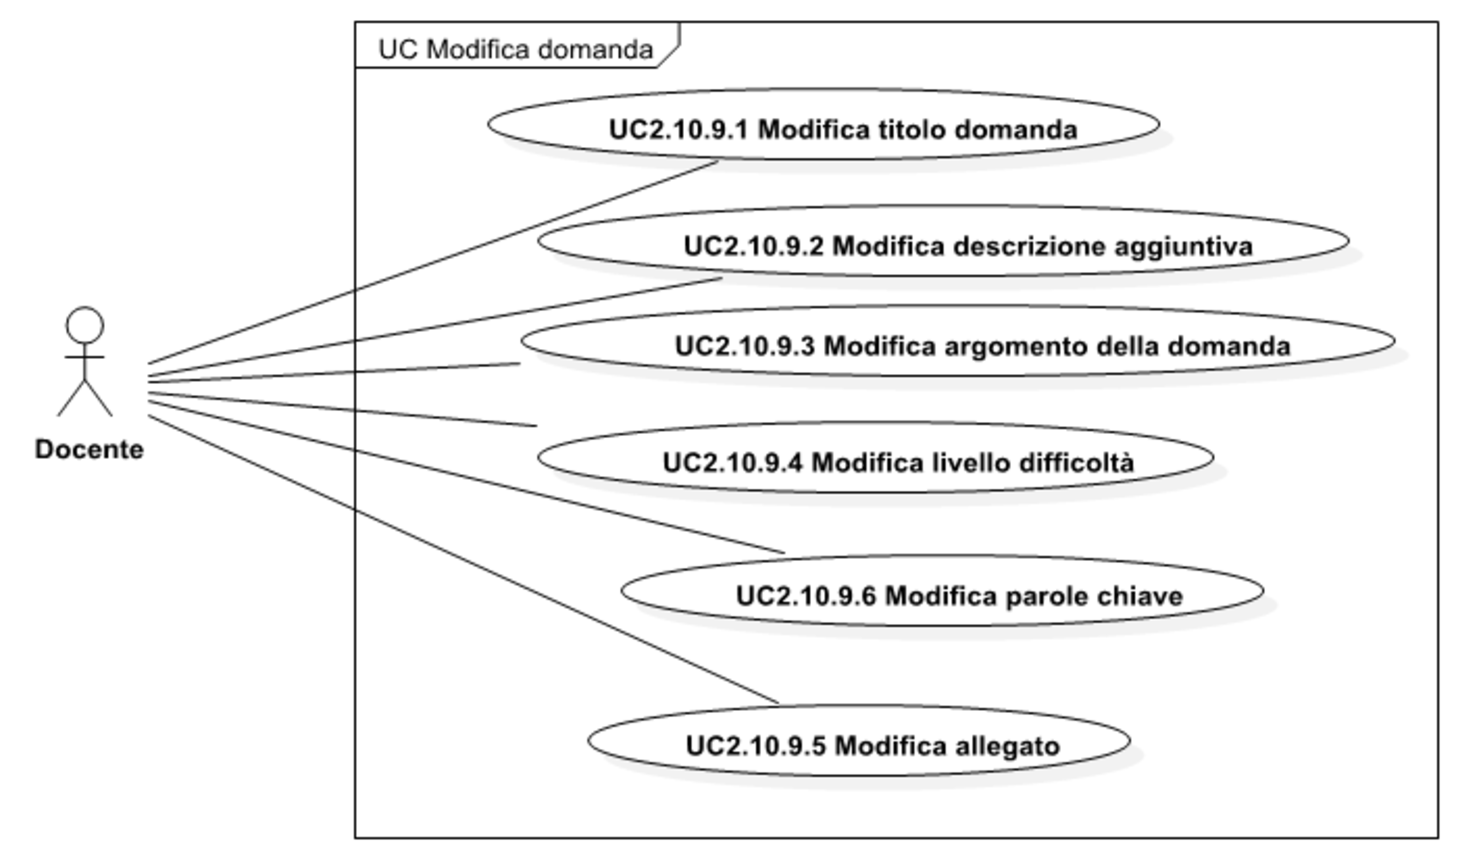
\includegraphics[width=\textwidth]{Img/UC Modifica domanda.pdf}}
\caption{UC2.11.9 Modifica domanda}
\end{figure}
\begin{itemize}
\item \textbf{Attori}: Docente.
\item \textbf{Scenario principale}:
\begin{enumerate}
\item Modifica titolo domanda
 (UC2.11.9.1);
\item Modifica descrizione aggiuntiva (UC2.11.9.2);
\item Modifica argomento della domanda (UC2.11.9.3);
\item Modifica livello difficoltà (UC2.11.9.4);
\item Modifica allegato (UC2.11.9.5).
\end{enumerate}
\item \textbf{Estensioni}:
\begin{itemize}
\item Errore numero risposte modifica (UC2.11.10);
\item Interruzione volontaria della modifica della domanda (UC2.11.11).
\end{itemize}
\item \textbf{Generalizzazioni}:
\begin{itemize}
\item Modifica domanda vero o falso (UC2.11.12);
\item Modifica domanda risposta multipla (UC2.11.13);
\item Modifica domanda a risposta aperta (UC2.11.14);
\item Modifica domanda a completamento testo (UC2.11.15);
\item Modifica domanda a collegamenti (UC2.11.16).
\end{itemize}
\item \textbf{Descrizione}: il docente deve poter modificare una domanda da lui creata.
\item \textbf{Precondizione}: il docente è stato riconosciuto e vuole modificare una domanda da lui creata
.
\item \textbf{Postcondizione}: il docente ha modificato una domanda esistente da lui creata.
\end{itemize}
\subsubsection{UC2.11.9.1 Modifica titolo domanda
}
\begin{itemize}
\item \textbf{Attori}: Docente.
\item \textbf{Scenario principale}: il docente può modificare il titolo della domanda che ha selezionato.
\item \textbf{Descrizione}: il docente deve poter modificare il titolo della domanda che ha selezionato.
\item \textbf{Precondizione}: il docente ha iniziato la modifica di una domanda ma non ha ancora modificato il titolo
.
\item \textbf{Postcondizione}: il docente ha modificato il titolo della domanda.
\end{itemize}
\subsubsection{UC2.11.9.2 Modifica descrizione aggiuntiva}
\begin{itemize}
\item \textbf{Attori}: Docente.
\item \textbf{Scenario principale}: il docente può modificare la descrizione aggiuntiva della domanda selezionata.
\item \textbf{Descrizione}: il docente deve poter modificare la descrizione aggiuntiva della domanda selezionata.
\item \textbf{Precondizione}: il docente ha iniziato la modifica di una domanda ma non ha ancora modificato la descrizione aggiuntiva.
\item \textbf{Postcondizione}: il docente ha modificato la descrizione aggiuntiva.
\end{itemize}
\subsubsection{UC2.11.9.3 Modifica argomento della domanda}
\begin{itemize}
\item \textbf{Attori}: Docente.
\item \textbf{Scenario principale}: il docente può modificare l'argomento della domanda selezionata semplicemente selezionando un argomento tra quelli disponibili.
\item \textbf{Descrizione}: il docente deve poter modificare l'argomento della domanda selezionata semplicemente selezionando un argomento tra quelli disponibili.
\item \textbf{Precondizione}: il docente ha iniziato la modifica di una domanda ma non ha ancora modificato l'argomento della domanda.
\item \textbf{Postcondizione}: il docente ha modificato l'argomento della domanda selezionata.
\end{itemize}
\subsubsection{UC2.11.9.4 Modifica livello difficoltà}
\begin{itemize}
\item \textbf{Attori}: Docente.
\item \textbf{Scenario principale}: il docente può modificare il livello di difficoltà della domanda selezionata.
\item \textbf{Descrizione}: il docente deve poter modificare il livello di difficoltà della domanda selezionata.
\item \textbf{Precondizione}: il docente ha iniziato la modifica di una domanda ma non ha ancora modificato il livello di difficoltà.
\item \textbf{Postcondizione}: il docente ha modificato il livello di difficoltà della domanda selezionata.
\end{itemize}
\subsubsection{UC2.11.9.5 Modifica allegato}
\begin{itemize}
\item \textbf{Attori}: Docente.
\item \textbf{Scenario principale}: il docente può modificare l'allegato della domanda eseguendo l'upload di un file multimediale (immagine, audio, video).
\item \textbf{Descrizione}: il docente ha la possibilità di modificare l'allegato della domanda eseguendo l'upload di un file multimediale.
\item \textbf{Precondizione}: il docente ha iniziato la modifica di una domanda ma non ha ancora modificato l'allegato della domanda.
\item \textbf{Postcondizione}: il docente ha modificato l'allegato della domanda.
\end{itemize}
\subsubsection{UC2.11.10 Errore numero risposte modifica}
\begin{itemize}
\item \textbf{Attori}: Docente.
\item \textbf{Scenario principale}: il docente durante la modifica di una domanda non ha lasciato un numero minimo di risposte valide.
\item \textbf{Descrizione}: il docente durante la modifica di una domanda non ha lasciato un numero minimo di risposte valide
.
\item \textbf{Precondizione}: il docente ha modificato una domanda ed ha un numero di risposte non valido.
\item \textbf{Postcondizione}: il docente visualizza il messaggio d'errore.
\end{itemize}
\subsubsection{UC2.11.11 Interruzione volontaria della modifica della domanda}
\begin{itemize}
\item \textbf{Attori}: Docente.
\item \textbf{Scenario principale}: il docente interrompe la modifica della domanda.
\item \textbf{Descrizione}: il docente sta modificando una domanda, ma interrompe volontariamente la modifica.
\item \textbf{Precondizione}: il docente sta modificando una domanda.
\item \textbf{Postcondizione}: la modifica della domanda è stata interrotta.
\end{itemize}
\subsubsection{UC2.11.12 Modifica domanda vero o falso}
\begin{figure}[H]
\centering
\noindent\makebox[\textwidth]{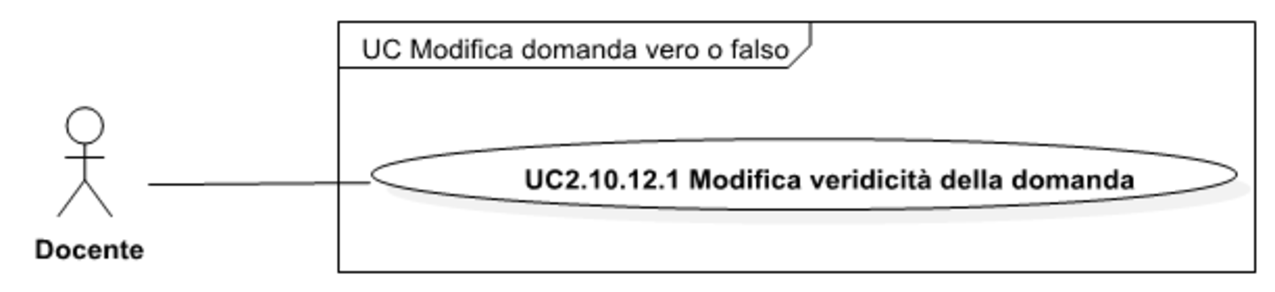
\includegraphics[width=\textwidth]{Img/UC Modifica domanda vero o falso.pdf}}
\caption{UC2.11.12 Modifica domanda vero o falso}
\end{figure}
\begin{itemize}
\item \textbf{Attori}: Docente.
\item \textbf{Scenario principale}:
\begin{enumerate}
\item Modifica veridicità della domanda (UC2.11.12.1).
\end{enumerate}
\item \textbf{Descrizione}: il docente deve poter modificare una domanda del tipo vero o falso da lui creata.
\item \textbf{Precondizione}: il docente è stato riconosciuto e vuole modificare una domanda vero o falso da lui creata.
\item \textbf{Postcondizione}: il docente ha modificato una domanda del tipo vero o falso esistente da lui creata.
\item \textbf{Specializzazione di}:
\begin{enumerate}
\item Modifica domanda (UC2.11.9).
\end{enumerate}
\end{itemize}
\subsubsection{UC2.11.12.1 Modifica veridicità della domanda}
\begin{itemize}
\item \textbf{Attori}: Docente.
\item \textbf{Scenario principale}: il docente deve poter modificare la veridicità della domanda che sta modificando.
\item \textbf{Descrizione}: il docente può modificare la veridicità della domanda che sta modificando.
\item \textbf{Precondizione}: il docente ha iniziato la modifica di una domanda del tipo vero o falso ma non ha ancora modificato la veridicità della domanda.
\item \textbf{Postcondizione}: il docente ha modificato la veridicità della domanda.
\end{itemize}
\subsubsection{UC2.11.13 Modifica domanda risposta multipla}
\begin{figure}[H]
\centering
\noindent\makebox[\textwidth]{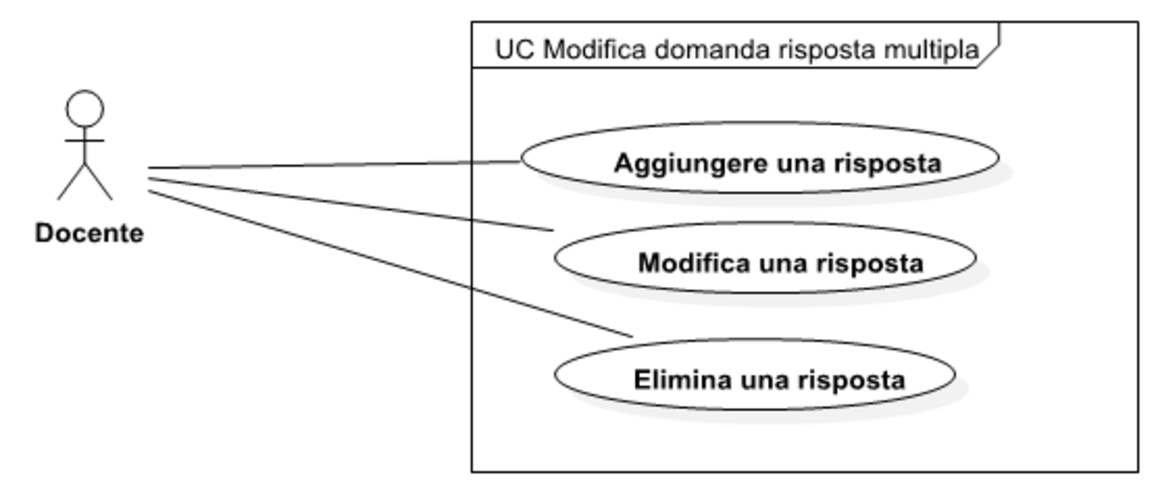
\includegraphics[width=\textwidth]{Img/UC Modifica domanda risposta multipla.pdf}}
\caption{UC2.11.13 Modifica domanda risposta multipla}
\end{figure}
\begin{itemize}
\item \textbf{Attori}: Docente.
\item \textbf{Scenario principale}:
\begin{enumerate}
\item Aggiungere una risposta (UC2.11.13.1);
\item Modificare una risposta (UC2.11.13.2);
\item Eliminare una risposta (UC2.11.13.3).
\end{enumerate}
\item \textbf{Descrizione}: il docente deve poter modificare una domanda a risposta multipla da lui creata.
\item \textbf{Precondizione}: il docente è stato riconosciuto e vuole modificare una domanda a risposta multipla da lui creata.
\item \textbf{Postcondizione}: il docente ha modificato una domanda a risposta multipla.
\item \textbf{Specializzazione di}:
\begin{enumerate}
\item Modifica domanda (UC2.11.9).
\end{enumerate}
\end{itemize}
\subsubsection{UC2.11.13.1 Aggiungere una risposta}
\begin{figure}[H]
\centering
\noindent\makebox[\textwidth]{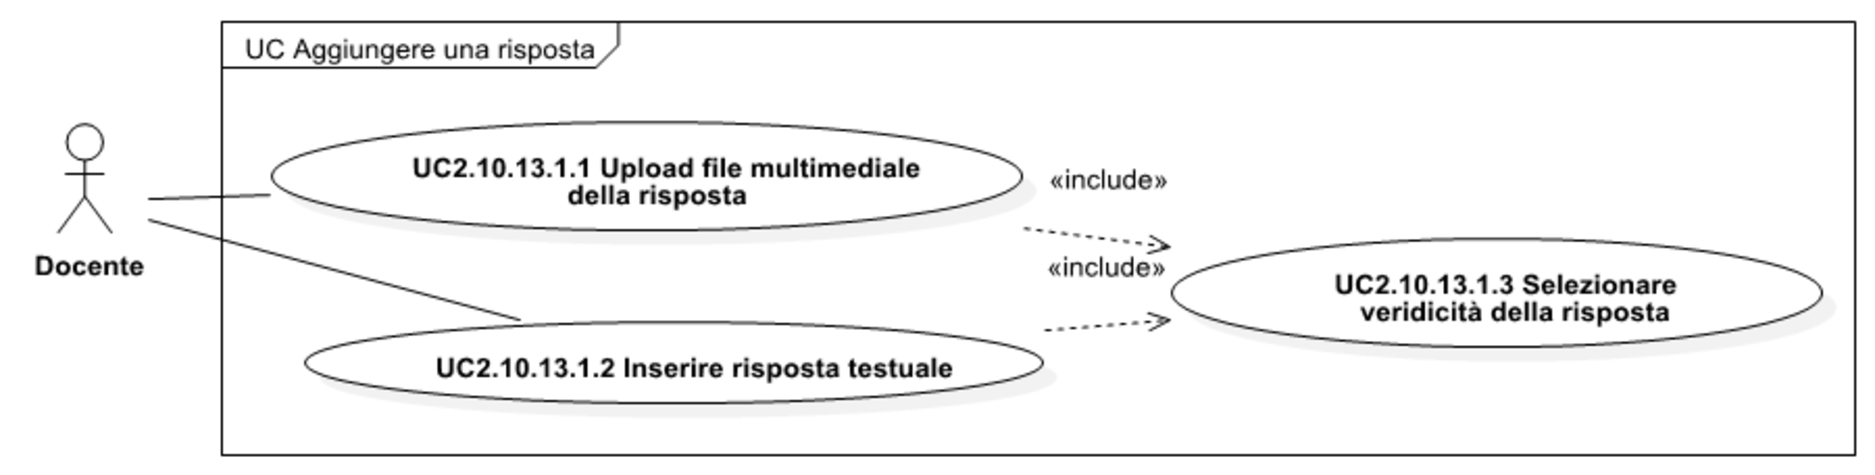
\includegraphics[width=\textwidth]{Img/UC Aggiungere una risposta.pdf}}
\caption{UC2.11.13.1 Aggiungere una risposta}
\end{figure}
\begin{itemize}
\item \textbf{Attori}: Docente.
\item \textbf{Scenario principale}:
\begin{enumerate}
\item Upload file multimediale della risposta (UC2.11.13.1.1);
\item Inserimento risposta testuale (UC2.11.13.1.2);
\item Selezione veridicità della risposta (UC2.11.13.1.3).
\end{enumerate}
\item \textbf{Descrizione}: il docente può aggiungere una nuova risposta alla domanda che sta modificando.
\item \textbf{Precondizione}: il docente ha iniziato la modifica di una domanda a risposta multipla ma non ha ancora aggiunto una nuova risposta.
\item \textbf{Postcondizione}: il docente ha aggiunto la nuova risposta.
\end{itemize}
\subsubsection{UC2.11.13.1.1 Upload file multimediale della risposta}
\begin{itemize}
\item \textbf{Attori}: Docente.
\item \textbf{Scenario principale}: il docente esegue l'upload di una immagine o di un video o di un file audio.
\item \textbf{Inclusioni}:
\begin{itemize}
\item Selezione veridicità della risposta (UC2.11.13.1.3).
\end{itemize}
\item \textbf{Descrizione}: il docente deve poter eseguire l'upload di una immagine o di un video o di un file audio.
\item \textbf{Precondizione}: il docente sta inserendo una nuova risposta  ma non ha ancora eseguito l'upload del file multimediale.
\item \textbf{Postcondizione}: il docente ha eseguito l'upload del file multimediale della risposta.
\end{itemize}
\subsubsection{UC2.11.13.1.2 Inserimento risposta testuale}
\begin{itemize}
\item \textbf{Attori}: Docente.
\item \textbf{Scenario principale}: il docente inserisce la risposta testuale.
\item \textbf{Inclusioni}:
\begin{itemize}
\item Selezione veridicità della risposta (UC2.11.13.1.3).
\end{itemize}
\item \textbf{Descrizione}: il docente deve poter inserire la risposta testuale.
\item \textbf{Precondizione}: il docente sta inserendo una nuova risposta ma non ha ancora inserito la risposta testuale.
\item \textbf{Postcondizione}: il docente ha inserito la risposta testuale.
\end{itemize}
\subsubsection{UC2.11.13.1.3 Selezione veridicità della risposta}
\begin{itemize}
\item \textbf{Attori}: Docente.
\item \textbf{Scenario principale}: il docente seleziona la veridicità della risposta che ha aggiunto.
\item \textbf{Descrizione}: il docente deve selezionare la veridicità della risposta che ha aggiunto.
\item \textbf{Precondizione}: il docente sta inserendo una nuova risposta ma non ha ancora selezionato la veridicità della risposta.
\item \textbf{Postcondizione}: il docente ha selezionato la veridicità della risposta.
\end{itemize}
\subsubsection{UC2.11.13.2 Modificare una risposta}
\begin{figure}[H]
\centering
\noindent\makebox[\textwidth]{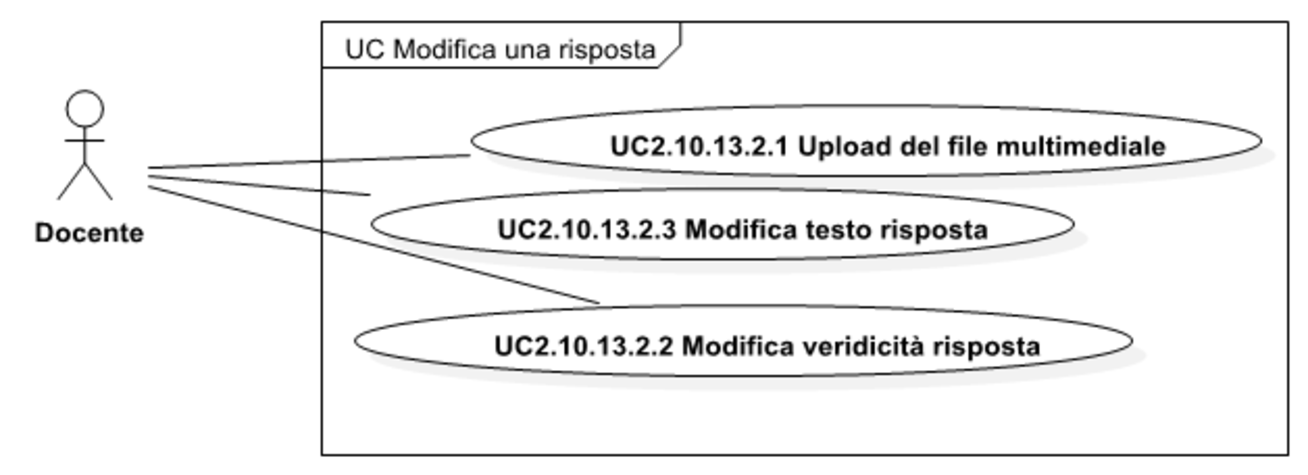
\includegraphics[width=\textwidth]{Img/UC Modificare una risposta.pdf}}
\caption{UC2.11.13.2 Modificare una risposta}
\end{figure}
\begin{itemize}
\item \textbf{Attori}: Docente.
\item \textbf{Scenario principale}:
\begin{enumerate}
\item Upload del file multimediale (UC2.11.13.2.1);
\item Modifica veridicità risposta (UC2.11.13.2.2);
\item Modifica testo risposta (UC2.11.13.2.3).
\end{enumerate}
\item \textbf{Descrizione}: il docente può modificare una risposta della domanda a risposta multipla.
\item \textbf{Precondizione}: il docente ha iniziato la modifica di una domanda a risposta multipla ma non ha ancora modificato una risposta.
\item \textbf{Postcondizione}: il docente ha modificato una risposta della domanda a risposta multipla.
\end{itemize}
\subsubsection{UC2.11.13.2.1 Upload del file multimediale}
\begin{itemize}
\item \textbf{Attori}: Docente.
\item \textbf{Scenario principale}: il docente sostituisce il file multimediale attuale della risposta con un altro eseguendo un upload del file.
\item \textbf{Inclusioni}:
\begin{itemize}
\item Selezione veridicità della risposta (UC2.11.5.1.3).
\end{itemize}
\item \textbf{Descrizione}: il docente può sostituire il file multimediale attuale della risposta con un altro eseguendo un upload del file
.
\item \textbf{Precondizione}: il docente sta modificando una risposta ma non ha ancora sostituito il file multimediale attuale della risposta.
\item \textbf{Postcondizione}: il docente ha eseguito l'upload sostituendo il file multimediale, della risposta, precedente.
\end{itemize}
\subsubsection{UC2.11.13.2.2 Modifica veridicità risposta}
\begin{itemize}
\item \textbf{Attori}: Docente.
\item \textbf{Scenario principale}: il docente modifica la veridicità della risposta.
\item \textbf{Descrizione}: il docente può modificare la veridicità della risposta.
\item \textbf{Precondizione}: il docente sta modificando una risposta ma non ha ancora cambiato la veridicità della risposta.
\item \textbf{Postcondizione}: il docente ha modificato la veridicità della risposta.
\end{itemize}
\subsubsection{UC2.11.13.2.3 Modifica testo risposta}
\begin{itemize}
\item \textbf{Attori}: Docente.
\item \textbf{Scenario principale}: il docente modifica la risposta testuale attuale.
\item \textbf{Descrizione}: il docente può modificare la risposta testuale attuale.
\item \textbf{Precondizione}: il docente sta modificando una risposta ma non ha ancora cambiato la risposta testuale.
\item \textbf{Postcondizione}: il docente ha modificato la risposta testuale.
\end{itemize}
\subsubsection{UC2.11.13.3 Eliminare una risposta}
\begin{itemize}
\item \textbf{Attori}: Docente.
\item \textbf{Scenario principale}: il docente elimina la risposta della domanda a risposta multipla.
\item \textbf{Descrizione}: il docente deve poter eliminare una risposta dalla domanda a risposta multipla da lui creata.
\item \textbf{Precondizione}: il docente sta modificando una domanda a risposta multipla da lui creata ma non ha ancora eliminato una risposta.
\item \textbf{Postcondizione}: il docente ha eliminato una risposta dalla domanda che stava modificando.
\end{itemize}
\subsubsection{UC2.11.14 Modifica domanda a risposta aperta}
\begin{itemize}
\item \textbf{Attori}: Docente.
\item \textbf{Scenario principale}:
\begin{enumerate}
\item Modifica della risposta (UC2.11.14.1).
\end{enumerate}
\item \textbf{Descrizione}: il docente deve poter modificare una domanda a risposta aperta esistente, da lui creata.
\item \textbf{Precondizione}: il docente è stato riconosciuto e vuole modificare una domanda a risposta aperta esistente, da lui creata.
\item \textbf{Postcondizione}: il docente ha modificato la domanda a risposta aperta.
\item \textbf{Specializzazione di}:
\begin{enumerate}
\item Modifica domanda (UC2.11.9).
\end{enumerate}
\end{itemize}
\subsubsection{UC2.11.14.1 Modifica della risposta}
\begin{itemize}
\item \textbf{Attori}: Docente.
\item \textbf{Scenario principale}: il docente modifica la risposta corretta alla domanda.
\item \textbf{Descrizione}: il docente può modificare la risposta corretta alla domanda.
\item \textbf{Precondizione}: il docente ha iniziato la modifica di una domanda a risposta aperta ma non ha ancora modificato la risposta corretta.
\item \textbf{Postcondizione}: il docente ha modificato la risposta corretta della domanda a risposta aperta.
\end{itemize}
\subsubsection{UC2.11.15 Modifica domanda a completamento testo}
\begin{itemize}
\item \textbf{Attori}: Docente.
\item \textbf{Scenario principale}:
\begin{enumerate}
\item Modifica testo incompleto (UC2.11.15.1);
\item Modifica parole esistenti (UC2.11.15.2);
\item Elimina parole (UC2.11.15.3).
\end{enumerate}
\item \textbf{Descrizione}: il docente deve poter modificare una domanda a completamento testo da lui creata.
\item \textbf{Precondizione}: il docente è stato riconosciuto e vuole modificare una domanda a completamento testo da lui creata.
\item \textbf{Postcondizione}: il docente ha modificato una domanda a completamento testo, esistente, da lui creata.
\item \textbf{Specializzazione di}:
\begin{enumerate}
\item Modifica domanda (UC2.11.9).
\end{enumerate}
\end{itemize}
\subsubsection{UC2.11.15.1 Modifica testo incompleto}
\begin{itemize}
\item \textbf{Attori}: Docente.
\item \textbf{Scenario principale}: il docente modifica il testo incompleto della domanda, specificando gli spazi vuoti nel testo.
\item \textbf{Descrizione}: il docente deve poter modificare il testo incompleto della domanda, specificando gli spazi vuoti.
\item \textbf{Precondizione}: il docente ha iniziato la modifica di una domanda a completamento testo ma non ha ancora modificato il testo incompleto della domanda.
\item \textbf{Postcondizione}: il docente ha modificato il testo incompleto della domanda.
\end{itemize}
\subsubsection{UC2.11.15.2 Modifica parole esistenti}
\begin{itemize}
\item \textbf{Attori}: Docente.
\item \textbf{Scenario principale}: il docente modifica l'insieme di parole associate al testo incompleto.
\item \textbf{Descrizione}: il docente deve poter modificare l'insieme di parole associate al testo incompleto.
\item \textbf{Precondizione}: il docente ha iniziato la modifica di una domanda a completamento testo ma non ha ancora modificato l'insieme di parole associate al testo incompleto.
\item \textbf{Postcondizione}: il docente ha modificato l'insieme di parole associate al testo incompleto.
\end{itemize}
\subsubsection{UC2.11.15.3 Elimina parole}
\begin{itemize}
\item \textbf{Attori}: Docente.
\item \textbf{Scenario principale}: il docente può eliminare alcune parole associate al testo incompleto.
\item \textbf{Descrizione}: il docente deve poter eliminare alcune parole associate al testo incompleto.
\item \textbf{Precondizione}: il docente ha iniziato la modifica di una domanda a completamento testo ma non ha ancora eliminato alcune parole.
\item \textbf{Postcondizione}: il docente ha eliminato alcune parole associate al testo incompleto.
\end{itemize}
\subsubsection{UC2.11.16 Modifica domanda a collegamenti}
\begin{itemize}
\item \textbf{Attori}: Docente.
\item \textbf{Scenario principale}:
\begin{enumerate}
\item Inserire ennupla (UC2.11.16.1);
\item Elimina ennupla (UC2.11.16.2).
\end{enumerate}
\item \textbf{Descrizione}: il docente deve poter modificare una domanda a collegamenti esistente, da lui creata.
\item \textbf{Precondizione}: il docente è stato riconosciuto e vuole modificare una domanda a collegamenti esistente da lui creata.
\item \textbf{Postcondizione}: il docente ha modificato la domanda a collegamenti.
\item \textbf{Specializzazione di}:
\begin{enumerate}
\item Modifica domanda (UC2.11.9).
\end{enumerate}
\end{itemize}
\subsubsection{UC2.11.16.1 Inserire ennupla}
\begin{itemize}
\item \textbf{Attori}: Docente.
\item \textbf{Scenario principale}:
\begin{enumerate}
\item Aggiungere parte iniziale (UC2.11.16.1.1);
\item Aggiungere parte finale (UC2.11.16.1.2).
\end{enumerate}
\item \textbf{Descrizione}: il docente sta modificando una domanda a collegamenti e può inserire una nuova ennupla (risposta).
\item \textbf{Precondizione}: il docente sta modificando una domanda a collegamenti ma non ha ancora aggiunto l'ennupla.
\item \textbf{Postcondizione}: il docente ha aggiunto l'ennupla (risposta) che ha creato.
\end{itemize}
\subsubsection{UC2.11.16.1.1 Aggiungere parte iniziale}
\begin{itemize}
\item \textbf{Attori}: Docente.
\item \textbf{Scenario principale}:
\begin{enumerate}
\item Upload file parte iniziale (UC2.11.16.1.1.1);
\item Aggiungere testo parte iniziale (UC2.11.16.1.1.2).
\end{enumerate}
\item \textbf{Descrizione}: il docente deve poter aggiungere la parte iniziale della risposta.
\item \textbf{Precondizione}: il docente sto creando l'ennupla ma non ha ancora inserito la parte iniziale della risposta.
\item \textbf{Postcondizione}: il docente ha inserito la parte iniziale dell'ennupla.
\end{itemize}
\subsubsection{UC2.11.16.1.1.1 Upload file parte iniziale}
\begin{itemize}
\item \textbf{Attori}: Docente.
\item \textbf{Scenario principale}: il docente inserisce un file multimediale nella parte iniziale della risposta, facendo l'upload del file.
\item \textbf{Descrizione}: il docente deve poter inserire il file multimediale della parte iniziale della ennupla, eseguendo l'upload del file.
\item \textbf{Precondizione}: il docente ha iniziato ad aggiungere la parte iniziale della risposta ma non ha ancora eseguito l'upload del file multimediale.
\item \textbf{Postcondizione}: il docente ha eseguito l'upload del file multimediale.
\end{itemize}
\subsubsection{UC2.11.16.1.1.2 Aggiungere testo parte iniziale}
\begin{itemize}
\item \textbf{Attori}: Docente.
\item \textbf{Scenario principale}: il docente inserisce del testo nella parta iniziale dell'ennupla (risposta).
\item \textbf{Descrizione}: il docente deve poter inserire del testo nella parte iniziale della risposta.
\item \textbf{Precondizione}: il docente ha iniziato ad aggiungere la parte iniziale dell'ennupla, ma non ha ancora specificato il testo da inserire.
\item \textbf{Postcondizione}: il docente ha inserito il testo nella parte iniziale dell'ennupla.
\end{itemize}
\subsubsection{UC2.11.16.1.2 Aggiungere parte finale}
\begin{itemize}
\item \textbf{Attori}: Docente.
\item \textbf{Scenario principale}:
\begin{enumerate}
\item Upload file parte finale (UC2.11.16.1.2.1);
\item Aggiungere testo parte finale (UC2.11.16.1.2.2).
\end{enumerate}
\item \textbf{Descrizione}: il docente deve poter aggiungere la parte finale della risposta.
\item \textbf{Precondizione}: il docente sta creando l'ennupla ma non ha ancora inserito la parte finale della risposta.
\item \textbf{Postcondizione}: il docente ha inserito la parte finale dell'ennupla.
\end{itemize}
\subsubsection{UC2.11.16.1.2.1 Upload file parte finale}
\begin{itemize}
\item \textbf{Attori}: Docente.
\item \textbf{Scenario principale}: il docente aggiunge un file multimediale nella parte finale della risposta, facendo l'upload del file.
\item \textbf{Descrizione}: il docente deve poter inserire il file multimediale nella parte finale della ennupla, eseguendo l'upload del file.
\item \textbf{Precondizione}: il docente ha iniziato ad aggiungere la parte finale della risposta ma non ha ancora eseguito l'upload del file multimediale.
\item \textbf{Postcondizione}: il docente ha eseguito l'upload del file multimediale.
\end{itemize}
\subsubsection{UC2.11.16.1.2.2 Aggiungere testo parte finale}
\begin{itemize}
\item \textbf{Attori}: Docente.
\item \textbf{Scenario principale}: il docente inserisce del testo nella parta finale dell'ennupla (risposta).
\item \textbf{Descrizione}: il docente deve poter inserire del testo nella parte finale della risposta.
\item \textbf{Precondizione}: il docente ha iniziato ad aggiungere la parte finale dell'ennupla, ma non ha ancora specificato il testo da inserire.
\item \textbf{Postcondizione}: il docente ha inserito il testo nella parte finale dell'ennupla.
\end{itemize}
\subsubsection{UC2.11.16.2 Elimina ennupla}
\begin{itemize}
\item \textbf{Attori}: Docente.
\item \textbf{Scenario principale}: il docente elimina una risposta dalla domanda a collegamenti.
\item \textbf{Descrizione}: il docente deve poter eliminare una risposta (ennupla) dalla domanda a collegamenti da lui creata.
\item \textbf{Precondizione}: il docente ha iniziato a modificare una domanda a collegamenti ma non ha ancora eliminato una ennupla (risposta).
\item \textbf{Postcondizione}: il docente ha eliminato una ennupla dalla domanda a collegamenti.
\end{itemize}


\setcounter{secnumdepth}{5} 
\setcounter{tocdepth}{5} 

\section{Specifica dei requisiti}
I requisiti saranno descritti nel seguente modo: R[importanza][tipo][id], con importanza=[O (obbligatorio), D (desiderabile), Z (opzionale)], id=codice univoco, tipo=[F (funzionale), Q (qualitativo), P (prestazionale), V (vincolante)].

\bigskip

I requisiti sono stati suddivisi in:
\begin{itemize}
\item \bold{obbligatori}: requisiti irrinunciabili per il corretto funzionamento del sistema;
\item \bold{desiderabili}: requisiti non irrinunciabili ma con un valore aggiunto riconoscibile;
\item \bold{opzionali}: requisiti di importanza relativa.
\end{itemize}

\bigskip

Per ogni requisito saranno specificati:
\begin{itemize}
\item titolo;
\item descrizione;
\item fonte.
\end{itemize}

\subsection{Requisiti funzionali}
I requisiti funzionali descrivono la funzionalità e il comportamento del prodotto, e determinano le capacità di calcolo richieste dal sistema. Devono essere verificabili attraverso test, dimostrazioni formali e revisioni.

\begin{tabella}{l!{\VRule}>{\centering\arraybackslash}p{3 cm}!{\VRule}>{\centering\arraybackslash}p{6 cm}!{\VRule}>{\centering\arraybackslash}p{2.5 cm}}
\color{white} \bold{Requisito} & \color{white} \bold{Tipologia} & \color{white} \bold{Descrizione} & \color{white} \bold{Fonti} \\
\endhead
ROF1 & Funzionale \linebreak obbligatorio & Un utente deve poter creare un account per usufruire delle funzionalità offerte dal sistema agli utenti registrati & UC1.1 \linebreak interna \\
ROF1.1 & Funzionale \linebreak obbligatorio & La registrazione richiede l'inserimento del nome dell'utente & UC1.1.1 \linebreak interna \\
ROF1.2 & Funzionale \linebreak obbligatorio & La registrazione richiede l'inserimento del cognome dell'utente & UC1.1.2 \linebreak interna \\
ROF1.3 & Funzionale \linebreak obbligatorio & La registrazione richiede l'inserimento dell'indirizzo email dell'utente & UC1.1.3 \linebreak interna \\
ROF1.3.1 & Funzionale \linebreak obbligatorio & L'indirizzo email inserito dall'utente deve avere un formato valido (*@*.*) & UC1.1.4 \linebreak interna \\
ROF1.3.2 & Funzionale \linebreak obbligatorio & L'indirizzo email inserito dall'utente deve essere univoco nel sistema & UC1.1.4 \linebreak interna \\
ROF1.3.3 & Funzionale \linebreak obbligatorio & Il sistema richiede di immettere una seconda volta l'indirizzo email precedentemente inserito  & UC1.1.4 \linebreak interna \\
ROF1.4 & Funzionale \linebreak obbligatorio & La registrazione richiede l'inserimento di una password & UC1.1.5 \linebreak interna \\
ROF1.4.1 & Funzionale \linebreak obbligatorio & La lunghezza della password inserita deve essere compresa fra 8 e 16 caratteri & UC1.1.5 \linebreak interna \\
ROF1.4.2 & Funzionale \linebreak obbligatorio & Il sistema richiede di immettere una seconda volta la password precedentemente inserita & UC1.1.6 \linebreak interna \\
ROF1.5 & Funzionale \linebreak obbligatorio & Il sistema notifica l'utente se è avvenuto un errore durante la registrazione & UC1.2 \linebreak interna \\
ROF2 & Funzionale \linebreak obbligatorio & Un utente registrato deve potersi autenticare nel sistema & UC1.3 \linebreak interna \\
ROF2.1 & Funzionale \linebreak obbligatorio & L'autenticazione richiede l'inserimento dell'indirizzo email dell'utente & UC1.3.1 \linebreak interna \\
ROF2.2 & Funzionale \linebreak obbligatorio & L'autenticazione richiede l'inserimento della password dell'utente & UC1.3.2 \linebreak interna \\
ROF2.3 & Funzionale \linebreak obbligatorio & Il sistema notifica l'utente se è avvenuto un errore durante l'autenticazione & UC1.4 \linebreak interna \\
ROF3 & Funzionale \linebreak obbligatorio & Un utente deve poter effettuare una richiesta di recupero password & UC1.5 \linebreak interna \\
ROF3.1 & Funzionale \linebreak obbligatorio & Il recupero della password richiede l'inserimento dell'indirizzo email dell'utente & UC1.5.1 \linebreak interna \\
ROF3.2 & Funzionale \linebreak obbligatorio & Il sistema notifica l'utente se è avvenuto un errore durante il recupero della password & UC1.6 \linebreak interna \\
ROF11 & Funzionale \linebreak obbligatorio & L'utente ha la possibilità di svolgere i quiz pubblici presenti su Quizzipedia & UC1.7 \linebreak capitolato \\
ROF11.1 & Funzionale \linebreak obbligatorio & L'utente seleziona il quiz che vuole svolgere tramite la ricerca fornita dal sistema & UC1.7.1 \linebreak interna \\
ROF11.1.1 & Funzionale \linebreak obbligatorio & L'utente cerca i quiz per argomento & interna \\
ROF11.1.2 & Funzionale \linebreak obbligatorio & L'utente cerca i quiz per livello di difficoltà
 & interna \\
ROF11.1.3 & Funzionale \linebreak obbligatorio & L'utente cerca i quiz per parola chiave
 & interna \\
ROF11.2 & Funzionale \linebreak obbligatorio & L'utente conferma la selezione del quiz precedentemente cercato & UC1.7.2 \linebreak interna \\
ROF11.3 & Funzionale \linebreak obbligatorio & L'utente risolve le domande poste nel quiz. L'utente può risolvere la stessa domanda più volte, sovrascrivendo la risposta precedente. 
L'utente può spostarsi a piacimento fra le domande del quiz. & UC1.7.3 \linebreak capitolato \\
ROF11.3.1 & Funzionale \linebreak obbligatorio & L'utente puo risolvere la stessa domanda piu volte, sovrascrivendo la risposta precedente
 & interna \\
ROF11.3.2 & Funzionale \linebreak obbligatorio & L'utente puo spostarsi a piacimento fra le domande del quiz & interna \\
ROF11.4 & Funzionale \linebreak obbligatorio & L'utente conferma la risoluzione del quiz. Dopo la consegna non sarà più possibile modificare le risposte e il quiz sarà valutato & UC1.7.4 \linebreak interna \\
ROF11.5 & Funzionale \linebreak obbligatorio & L'utente visualizza l'esito del quiz svolto & UC1.7.5 \linebreak interna \\
ROF12 & Funzionale \linebreak obbligatorio & Il sistema mette a disposizione dell'utente una funzionalità di ricerca quiz e domande & UC1.8 \linebreak interna \\
ROF12.1 & Funzionale \linebreak obbligatorio & Utenti e utenti autenticati devono poter effettuare ricerche di quiz e visualizzarne i risultati & UC1.8 \linebreak interna \\
ROF12.1.1 & Funzionale \linebreak obbligatorio & Utenti e utenti autenticati devono poter personalizzare la ricerca dei quiz attraverso vari parametri & interna \\
ROF12.1.1.1 & Funzionale \linebreak obbligatorio & Utenti e utenti autenticati devono poter limitare la ricerca di quiz per argomento & interna \\
ROF12.1.1.2 & Funzionale \linebreak obbligatorio & Utenti e utenti autenticati devono poter limitare la ricerca di quiz per livello di difficoltà & interna \\
ROF12.1.1.3 & Funzionale \linebreak obbligatorio & Utenti e utenti autenticati devono poter limitare la ricerca di quiz per parole chiave & interna \\
ROF12.1.1.4 & Funzionale \linebreak obbligatorio & Utenti e utenti autenticati devono poter limitare la ricerca di quiz visualizzando solo quiz pubblici & interna \\
ROF12.1.1.5 & Funzionale \linebreak obbligatorio & Gli studenti possono limitare la ricerca di quiz visualizzando solo quiz privati & interna \\
ROF12.1.1.5.1 & Funzionale \linebreak obbligatorio & Gli studenti possono limitare la ricerca di quiz, visualizzando solo quiz appartenenti a un ente a cui appartengono & interna \\
ROF12.1.1.5.1.1 & Funzionale \linebreak obbligatorio & Gli studenti possono limitare la ricerca di quiz, visualizzando solo quiz appartenenti a una classe a cui appartengono & interna \\
ROF12.1.1.6 & Funzionale \linebreak obbligatorio & Utenti e utenti autenticati devono poter limitare la ricerca di quiz per autore del quiz & interna \\
ROF12.2 & Funzionale \linebreak obbligatorio & I docenti devono poter effettuare ricerche di domande e visualizzarne i risultati & UC1.8 \linebreak interna \\
ROF12.2.1 & Funzionale \linebreak obbligatorio & I docenti devono poter personalizzare la ricerca delle domande attraverso vari parametri & interna \\
ROF12.2.1.1 & Funzionale \linebreak obbligatorio & I docenti devono poter limitare la ricerca di domande per argomento & interna \\
ROF12.2.1.2 & Funzionale \linebreak obbligatorio & I docenti devono poter limitare la ricerca di domande per livello di difficoltà & interna \\
ROF12.2.1.3 & Funzionale \linebreak obbligatorio & I docenti devono poter limitare la ricerca di domande per parole chiave & interna \\
ROF12.2.1.4 & Funzionale \linebreak obbligatorio & I docenti devono poter limitare la ricerca di domande per autore & interna \\
ROF13 & Funzionale \linebreak obbligatorio & L'utente autenticato quando vorrà terminare la navigazione su Quizzipedia potrà effettuare il logout dal sistema & UC2.1 \linebreak interna \\
ROF14 & Funzionale \linebreak obbligatorio & Il sistema deve mettere a disposizione dell'utente delle funzionalità per la gestione del proprio account & UC2.4 \linebreak interna \\
ROF14.1 & Funzionale \linebreak obbligatorio & L'utente autenticato deve poter visualizzare le sue informazioni personali & UC2.4.1 \linebreak interna \\
ROF14.1.1 & Funzionale \linebreak obbligatorio & L'utente autenticato deve poter visualizzare il suo nome & UC2.4.1.1 \linebreak interna \\
ROF14.1.2 & Funzionale \linebreak obbligatorio & L'utente autenticato deve poter visualizzare il suo cognome & UC2.4.1.2 \linebreak interna \\
ROF14.1.3 & Funzionale \linebreak obbligatorio & L'utente autenticato deve poter visualizzare il suo indirizzo email & UC2.4.1.3 \linebreak interna \\
ROF14.2 & Funzionale \linebreak obbligatorio & L'utente autenticato deve poter visualizzare uno storico dei quiz da lui svolti & UC2.4.3 \linebreak capitolato \\
ROF14.3 & Funzionale \linebreak obbligatorio & L'utente autenticato deve poter modificare le sue informazioni personali & UC2.4.2 \linebreak interna \\
ROF14.3.1 & Funzionale \linebreak obbligatorio & L'utente autenticato deve poter modificare il suo nome & UC2.4.2.1 \linebreak interna \\
ROF14.3.2 & Funzionale \linebreak obbligatorio & L'utente autenticato deve poter modificare il suo cognome & UC2.4.2.2 \linebreak interna \\
ROF14.3.3 & Funzionale \linebreak obbligatorio & L'utente autenticato deve poter modificare la sua password & UC2.4.2.3 \linebreak interna \\
ROF14.3.3.1 & Funzionale \linebreak obbligatorio & La modifica della password richiede l'inserimento della password corrente o di una password temporanea & UC2.4.2.3.1 \linebreak interna \\
ROF14.3.3.2 & Funzionale \linebreak obbligatorio & La modifica della password richiede l'inserimento della nuova password & UC2.4.2.3.2 \linebreak interna \\
ROF14.3.3.3 & Funzionale \linebreak obbligatorio & La modifica della password richiede di immettere una seconda volta la nuova password & UC2.4.2.3.3 \linebreak interna \\
ROF14.3.3.4 & Funzionale \linebreak obbligatorio & Il sistema notifica l'utente se è avvenuto un errore durante la modifica della password & UC2.4.2.4 \linebreak interna \\
ROF14.4 & Funzionale \linebreak obbligatorio & Il sistema mette a disposizione funzionalità di eliminazione degli account & UC2.4.4 \linebreak interna \\
ROF14.4.1 & Funzionale \linebreak obbligatorio & L'utente autenticato deve poter eliminare il proprio account & UC2.4.5 \linebreak interna \\
ROF14.4.2 & Funzionale \linebreak obbligatorio & Il responsabile deve poter eliminare l'account degli utenti da lui gestiti & UC2.4.6 \linebreak interna \\
ROF15 & Funzionale \linebreak obbligatorio & Il sistema mette a disposizione del docente funzionalità di gestione dei quiz & UC2.2 \linebreak capitolato \\
ROF15.1 & Funzionale \linebreak obbligatorio & Il docente deve poter creare un nuovo quiz & UC2.2.1 \linebreak capitolato \\
ROF15.1.1 & Funzionale \linebreak obbligatorio & La creazione del quiz richiede l'inserimento del titolo del quiz & UC2.2.1.1 \linebreak interna \\
ROF15.1.2 & Funzionale \linebreak obbligatorio & La creazione del quiz richiede la selezione dell'argomento del quiz & UC2.2.1.2 \linebreak interna \\
ROF15.1.3 & Funzionale \linebreak obbligatorio & La creazione del quiz richiede l'inserimento della descrizione del quiz & UC2.2.1.3 \linebreak interna \\
ROF15.1.4 & Funzionale \linebreak obbligatorio & La creazione del quiz richiede la selezione del permesso del quiz (pubblico o privato) & UC2.2.1.4 \linebreak interna \\
ROF15.1.5 & Funzionale \linebreak obbligatorio & Il docente deve poter inserire domande nel quiz che sta creando & UC2.2.1.5 \linebreak interna \\
ROF15.1.6 & Funzionale \linebreak obbligatorio & Il docente deve poter rimuovere domande dal quiz che sta creando & UC2.2.1.6 \linebreak interna \\
ROF15.2 & Funzionale \linebreak obbligatorio & Il docente deve poter modificare un quiz esistente & UC2.2.2 \linebreak capitolato \\
ROF15.2.1 & Funzionale \linebreak obbligatorio & Il docente può modificare il titolo del quiz & UC2.2.2.4 \linebreak interna \\
ROF15.2.2 & Funzionale \linebreak obbligatorio & Il docente può modificare l'argomento del quiz & UC2.2.2.5 \linebreak interna \\
ROF15.2.3 & Funzionale \linebreak obbligatorio & Il docente può modificare la descrizione del quiz & UC2.2.2.6 \linebreak interna \\
ROF15.2.4 & Funzionale \linebreak obbligatorio & Il docente può specificare e modificare il permesso del quiz & UC2.2.2.1 \linebreak interna \\
ROF15.2.4.1 & Funzionale \linebreak obbligatorio & Il docente può specificare un permesso 'pubblico' per il quiz & UC2.2.2.1.1 \linebreak interna \\
ROF15.2.4.2 & Funzionale \linebreak obbligatorio & Il docente può specificare un permesso 'privato' per il quiz  & UC2.2.2.1.2 \linebreak interna \\
ROF15.2.4.2.1 & Funzionale \linebreak obbligatorio & Il docente può specificare una o più classi a cui permette lo svolgimento del quiz & UC2.2.2.1.2.1 \linebreak interna \\
ROF15.2.5 & Funzionale \linebreak obbligatorio & il docente deve poter inserire una domanda nel quiz & UC2.2.2.2 \linebreak capitolato \\
ROF15.2.5.1 & Funzionale \linebreak obbligatorio & Il docente può cercare una domanda esistente e inserirla nel quiz & UC1.8 \linebreak interna \\
ROF15.2.5.2 & Funzionale \linebreak obbligatorio & Il docente può creare una nuova domanda e inserirla nel quiz & interna \\
ROF15.2.6 & Funzionale \linebreak obbligatorio & Il docente deve poter rimuovere una domanda dal quiz & UC2.2.2.3 \linebreak interna \\
ROF15.2.7 & Funzionale \linebreak obbligatorio & Il sistema notifica l'utente se si è verificato un errore durante la modifica del quiz & UC2.2.3 \linebreak interna \\
ROF15.3 & Funzionale \linebreak obbligatorio & Il docente deve poter eliminare un quiz & UC2.2.4 \linebreak capitolato \\
ROF16 & Funzionale \linebreak obbligatorio & L'utente senza ruolo, lo studente e il docente possono effettuare varie richieste & UC2.5 \linebreak interna \\
ROF16.1 & Funzionale \linebreak obbligatorio & L'utente senza ruolo può richiedere di assumere il ruolo di docente & UC2.5.1 \linebreak interna \\
ROF16.2 & Funzionale \linebreak obbligatorio & L'utente senza ruolo può richiedere di assumere il ruolo di studente & UC2.5.2 \linebreak interna \\
ROF16.3 & Funzionale \linebreak obbligatorio & Il docente può effettuare una richiesta di accettazione di inserimento in una classe & UC2.5.3 \linebreak interna \\
ROF16.4 & Funzionale \linebreak obbligatorio & Lo studente può effettuare una richiesta di accettazione di inserimento in una classe & UC2.5.4 \linebreak interna \\
ROF17 & Funzionale \linebreak obbligatorio & Il responsabile e il docente devono poter gestire le richieste effettuate dagli utenti & UC2.9 \linebreak interna \\
ROF17.1 & Funzionale \linebreak obbligatorio & Il responsabile può gestire le richieste di inserimento dei docenti in una classe & UC2.9.1 \linebreak interna \\
ROF17.1.1 & Funzionale \linebreak obbligatorio & Il responsabile può accettare una richiesta di inserimento in una classe pervenuta da un docente & UC2.9.1.1 \linebreak interna \\
ROF17.1.2 & Funzionale \linebreak obbligatorio & Il responsabile può rifiutare la richiesta di inserimento in una classe pervenuta da un docente & UC2.9.1.2 \linebreak interna \\
ROF17.2 & Funzionale \linebreak obbligatorio & Il responsabile può gestire le richieste di attribuzione del ruolo di docente & UC2.9.2 \linebreak interna \\
ROF17.2.1 & Funzionale \linebreak obbligatorio & Il responsabile può accettare la richiesta di attribuzione del ruolo di docente & UC2.9.2.1 \linebreak interna \\
ROF17.2.2 & Funzionale \linebreak obbligatorio & Il responsabile può rifiutare la richiesta di attribuzione del ruolo di docente & UC2.9.2.2 \linebreak interna \\
ROF17.3 & Funzionale \linebreak obbligatorio & Il docente può gestire le richieste di inserimento degli studenti in una classe & UC2.9.3 \linebreak interna \\
ROF17.3.1 & Funzionale \linebreak obbligatorio & Il docente può accettare una richiesta di inserimento in una classe pervenuta da uno studente & UC2.9.3.1 \linebreak interna \\
ROF17.3.2 & Funzionale \linebreak obbligatorio & Il docente può rifiutare una richiesta di inserimento in una classe pervenuta da uno studente & UC2.9.3.2 \linebreak interna \\
ROF17.4 & Funzionale \linebreak obbligatorio & Il docente può gestire le richieste di attribuzione del ruolo di studente & UC2.9.4 \linebreak interna \\
ROF17.4.1 & Funzionale \linebreak obbligatorio & Il docente può accettare la richiesta di attibuzione del ruolo di studente & UC2.9.4.1 \linebreak interna \\
ROF17.4.2 & Funzionale \linebreak obbligatorio & Il docente può rifiutare la richiesta di attibuzione del ruolo di studente & UC2.9.4.2 \linebreak interna \\
ROF18 & Funzionale \linebreak obbligatorio & Il sistema deve mettere a disposizione del docente delle funzionalità per la gestione degli argomenti & UC2.3 \linebreak interna \\
ROF18.1 & Funzionale \linebreak obbligatorio & Il docente deve poter creare un nuovo argomento & UC2.3.1 \linebreak interna \\
ROF18.1.1 & Funzionale \linebreak obbligatorio & La creazione di un nuovo argomento richiede l'inserimento del nome dell'argomento & UC2.3.1.1 \linebreak interna \\
ROF18.2 & Funzionale \linebreak obbligatorio & Il docente deve poter eliminare un argomento esistente & UC2.3.3 \linebreak interna \\
ROF19 & Funzionale \linebreak obbligatorio & Il sistema mette a disposizione del responsabile delle funzionalità di gestione ente & UC2.7 \linebreak interna \\
ROF19.1 & Funzionale \linebreak obbligatorio & Il responsabile deve poter creare un nuovo ente & UC2.7.1 \linebreak interna \\
ROF19.1.1 & Funzionale \linebreak obbligatorio & La creazione di un ente richiede l'inserimento della data di creazione dell'ente & UC2.7.1.1 \linebreak interna \\
ROF19.1.2 & Funzionale \linebreak obbligatorio & La creazione di un ente richiede l'inserimento del nome dell'ente & UC2.7.1.2 \linebreak interna \\
ROF19.2 & Funzionale \linebreak obbligatorio & Il responsabile deve poter modificare un ente esistente & UC2.7.2 \linebreak interna \\
ROF19.2.1 & Funzionale \linebreak obbligatorio & Il responsabile può modificare il nome dell'ente & UC2.7.2.1 \linebreak interna \\
ROF19.3 & Funzionale \linebreak obbligatorio & Il responsabile deve poter eliminare un ente esistente & UC2.7.3 \linebreak interna \\
ROF20 & Funzionale \linebreak obbligatorio & Il docente deve poter visualizzare delle statistiche di vario tipo & UC2.6 \linebreak interna \\
ROF20.1 & Funzionale \linebreak obbligatorio & Il docente deve poter visualizzare le statistiche relative ai quiz & UC2.6.1 \linebreak capitolato \\
ROF20.1.1 & Funzionale \linebreak obbligatorio & Il docente può visualizzare il numero di volte in cui un quiz è stato risolto & UC2.6.1.1 \linebreak interna \\
ROF20.1.2 & Funzionale \linebreak obbligatorio & Il docente può visualizzare la percentuale di superamento di ogni quiz & UC2.6.1.2 \linebreak interna \\
ROF20.1.2.1 & Funzionale \linebreak obbligatorio & Il docente può visualizzare il numero di quiz in cui compare la domanda & UC2.6.2.1 \linebreak interna \\
ROF20.1.3 & Funzionale \linebreak obbligatorio & Il docente può visualizzare il voto medio ottenuto dagli utenti in ogni quiz & UC2.6.1.3 \linebreak interna \\
ROF20.2 & Funzionale \linebreak obbligatorio & Il docente deve poter visualizzare le statistiche relative alle domande & UC2.6.2 \linebreak capitolato \\
ROF20.2.1 & Funzionale \linebreak obbligatorio & Il docente può visualizzare la percentuale di successo nella risposta alla domanda & UC2.6.2.2 \linebreak interna \\
ROF20.3 & Funzionale \linebreak obbligatorio & Il docente deve poter visualizzare le statistiche relative agli studenti & UC2.6.3 \linebreak capitolato \\
ROF20.3.1 & Funzionale \linebreak obbligatorio & Il docente può visualizzare la lista dei quiz svolti da ogni studente e il voto corrispondente & UC2.6.3.1 \linebreak interna \\
ROF21 & Funzionale \linebreak obbligatorio & Il sistema deve mettere a disposizione del responsabile delle funzionalità di gestione delle classi & UC2.8 \linebreak interna \\
ROF21.1 & Funzionale \linebreak obbligatorio & Il responsabile deve poter creare una classe & UC2.8.1 \linebreak interna \\
ROF21.1.1 & Funzionale \linebreak obbligatorio & La creazione della classe richiede l'inserimento del nome della classe & UC2.8.1.1 \linebreak interna \\
ROF21.1.2 & Funzionale \linebreak obbligatorio & La creazione della classe richiede l'inserimento della descrizione della classe & UC2.8.1.2 \linebreak interna \\
ROF21.1.3 & Funzionale \linebreak obbligatorio & La creazione della classe richiede la selezione dell'ente a cui appartiene la classe & interna \\
ROF21.1.4 & Funzionale \linebreak obbligatorio & La creazione della classe richiede l'inserimento dell'anno scolastico  & UC2.8.1.3 \linebreak interna \\
ROF21.2 & Funzionale \linebreak obbligatorio & Il responsabile deve poter modificare una classe & UC2.8.2 \linebreak interna \\
ROF21.2.1 & Funzionale \linebreak obbligatorio & Il responsabile può modificare il nome della classe & interna \\
ROF21.2.2 & Funzionale \linebreak obbligatorio & Il responsabile può modificare la descrizione della classe & UC2.8.2.1 \linebreak interna \\
ROF21.2.3 & Funzionale \linebreak obbligatorio & Il responsabile può modificare l'ente a cui la classe appartiene & interna \\
ROF21.2.4 & Funzionale \linebreak obbligatorio & Il responsabile può modificare l'anno scolastico & interna \\
ROF21.3 & Funzionale \linebreak obbligatorio & Il responsabile deve poter eliminare una classe & UC2.8.3 \linebreak interna \\
ROF21.4 & Funzionale \linebreak obbligatorio & Il docente deve poter visualizzare la lista degli studenti di una classe & UC2.8.4 \linebreak interna \\
ROF21.5 & Funzionale \linebreak obbligatorio & Il responsabile deve poter visualizzare la lista dei docenti di una classe & UC2.8.5 \linebreak interna \\
ROF21.6 & Funzionale \linebreak obbligatorio & Il responsabile deve poter effettuare la manutenzione di una classe & UC2.8.6 \linebreak interna \\
ROF21.6.1 & Funzionale \linebreak obbligatorio & Il responsabile può inserire uno studente nella classe & UC2.8.6.1 \linebreak interna \\
ROF21.6.2 & Funzionale \linebreak obbligatorio & Il responsabile può rimuovere uno studente dalla classe & UC2.8.6.2 \linebreak interna \\
ROF21.6.3 & Funzionale \linebreak obbligatorio & Il responsabile può inserire un docente nella classe & UC2.8.6.3 \linebreak interna \\
ROF21.6.4 & Funzionale \linebreak obbligatorio & Il responsabile può rimuovere un docente dalla classe & UC2.8.6.4 \linebreak interna \\
ROF31 & Funzionale \linebreak obbligatorio & Il sistema mette a disposizione del docente funzionalità di gestione delle domande & UC2.10 \linebreak capitolato \\
ROF31.1 & Funzionale \linebreak obbligatorio & Il docente deve poter creare una nuova domanda & UC2.10.1 \linebreak capitolato \\
ROF31.1.1 & Funzionale \linebreak obbligatorio & La creazione, di ogni domanda, richiede l'inserimento del titolo della domanda & UC2.10.1.1 \linebreak interna \\
ROF31.1.2 & Funzionale \linebreak obbligatorio & La creazione, di ogni tipo di domanda, richiede l'inserimento di una descrizione aggiuntiva & UC2.10.1.2 \linebreak interna \\
ROF31.1.3 & Funzionale \linebreak obbligatorio & La creazione, di ogni tipo di domanda, richiede la selezione dell'argomento della domanda & UC2.10.1.3 \linebreak interna \\
ROF31.1.4 & Funzionale \linebreak obbligatorio & La creazione, di ogni tipo di domanda, richiede la selezione del livello di difficoltà della domanda & UC2.10.1.4 \linebreak interna \\
ROF31.1.5 & Funzionale \linebreak obbligatorio & La creazione, di ogni tipo di domanda, permette l'inserimento facoltativo di un allegato & UC2.10.1.5 \linebreak interna \\
ROF31.2 & Funzionale \linebreak obbligatorio & Il docente può interrompere la creazione di qualsiasi domanda volontariamente & UC2.10.3 \linebreak interna \\
ROF31.3 & Funzionale \linebreak obbligatorio & Il docente deve poter creare una domanda di tipo vero o falso & UC2.10.4 \linebreak interna \\
ROF31.3.1 & Funzionale \linebreak obbligatorio & Il docente, durante la creazione di una domanda di tipo vero o falso, deve selezionare la veridicità della domanda & UC2.10.4.1 \linebreak interna \\
ROF31.4 & Funzionale \linebreak obbligatorio & Il docente deve poter creare una domanda a risposta aperta & UC2.10.7 \linebreak interna \\
ROF31.4.1 & Funzionale \linebreak obbligatorio & Il docente, durante la creazione di una domanda a risposta aperta, deve inserire la risposta corretta & UC2.10.7.1 \linebreak interna \\
ROF31.5 & Funzionale \linebreak obbligatorio & Il docente deve poter creare una domanda a risposta multipla & UC2.10.5 \linebreak interna \\
ROF31.5.1 & Funzionale \linebreak obbligatorio & Il docente, durante la creazione di una domanda a risposta multipla, deve poter creare una risposta & UC2.10.5.1 \linebreak interna \\
ROF31.5.1.1 & Funzionale \linebreak obbligatorio & Il docente, durante la creazione di una risposta a una domanda a risposta multipla, può selezionare una risposta testuale & UC2.10.5.1.2 \linebreak interna \\
ROF31.5.1.2 & Funzionale \linebreak obbligatorio & Il docente, durante la creazione di una risposta a una domanda a risposta multipla, può selezionare una risposta multimediale (immagine o video o audio) & UC2.10.5.1.1 \linebreak interna \\
ROF31.5.1.3 & Funzionale \linebreak obbligatorio & Il docente, durante la creazione di una risposta a una domanda a risposta multipla, deve selezionare la veridicità della risposta creata & UC2.10.5.1.3 \linebreak interna \\
ROF31.6 & Funzionale \linebreak obbligatorio & Il docente deve poter creare una domanda a completamento testo & UC2.10.8 \linebreak interna \\
ROF31.6.1 & Funzionale \linebreak obbligatorio & Il docente, durante la creazione di una domanda a completamento testo, deve inserire il testo incompleto della domanda, specificando gli spazi vuoti & UC2.10.8.1 \linebreak interna \\
ROF31.6.2 & Funzionale \linebreak obbligatorio & Il docente, durante la creazione di una domanda a completamento testo, deve specificare un insieme di parole che sono corrette e sbagliate & UC2.10.8.2 \linebreak interna \\
ROF31.7 & Funzionale \linebreak obbligatorio & Il docente deve poter creare una domanda a collegamenti & UC2.10.6 \linebreak interna \\
ROF31.7.1 & Funzionale \linebreak obbligatorio & Il docente, durante la creazione di una domanda a collegamenti, deve poter creare una ennupla (risposta) & UC2.10.6.1 \linebreak interna \\
ROF31.7.1.1 & Funzionale \linebreak obbligatorio & Il docente, durante la creazione di una ennupla della domanda a collegamenti, può specificare o no la parte iniziale della risposta & UC2.10.6.1.1 \linebreak interna \\
ROF31.7.1.1.1 & Funzionale \linebreak obbligatorio & Il docente, durante la creazione della parte iniziale della risposta della domanda a collegamenti, può inserire un file multimediale (immagine, audio, video) & UC2.10.6.1.1.1 \linebreak interna \\
ROF31.7.1.1.2 & Funzionale \linebreak obbligatorio & Il docente, durante la creazione della parte iniziale della risposta della domanda a collegamenti, può inserire il testo della risposta iniziale & UC2.10.6.1.1.2 \linebreak interna \\
ROF31.7.1.2 & Funzionale \linebreak obbligatorio & Il docente, durante la creazione di una ennupla della domanda a collegamenti, deve specificare la parte finale della risposta & UC2.10.6.1.2 \linebreak interna \\
ROF31.7.1.2.1 & Funzionale \linebreak obbligatorio & Il docente, durante la creazione della parte finale della risposta della domanda a collegamenti, può inserire un file multimediale (immagine, video, audio) & UC2.10.6.1.2.1 \linebreak interna \\
ROF31.7.1.2.2 & Funzionale \linebreak obbligatorio & Il docente, durante la creazione della parte finale della domanda a collegamenti, può inserire il testo della risposta finale & UC2.10.6.1.2.2 \linebreak interna \\
ROF31.8 & Funzionale \linebreak obbligatorio & Il docente deve poter modificare una domanda da lui creata & UC2.10.9 \linebreak interna \\
ROF31.8.1 & Funzionale \linebreak obbligatorio & Il docente, durante la modifica di ogni tipo di domanda, può modificare il titolo della domanda & UC2.10.9.1 \linebreak interna \\
ROF31.8.2 & Funzionale \linebreak obbligatorio & Il docente, durante la modifica di ogni tipo di domanda, può modificare la descrizione aggiuntiva & UC2.10.9.2 \linebreak interna \\
ROF31.8.3 & Funzionale \linebreak obbligatorio & Il docente, durante la modifica di ogni tipo di domanda, può modificare l'argomento della domanda & UC2.10.9.3 \linebreak interna \\
ROF31.8.4 & Funzionale \linebreak obbligatorio & Il docente, durante la modifica di ogni tipo di domanda, può modificare il livello di difficoltà della domanda & UC2.10.9.4 \linebreak interna \\
ROF31.8.5 & Funzionale \linebreak obbligatorio & Il docente, durante la modifica di ogni tipo di domanda, può modificare l'allegato precedentemente inserito & UC2.10.9.5 \linebreak interna \\
ROF31.9 & Funzionale \linebreak obbligatorio & Il docente può interrompere volontariamente la modifica di una domanda & UC2.10.11 \linebreak interna \\
ROF31.10 & Funzionale \linebreak obbligatorio & Il docente deve poter modificare una domanda di tipo vero o falso da lui creata & UC2.10.12 \linebreak interna \\
ROF31.10.1 & Funzionale \linebreak obbligatorio & Il docente, durante la modifica di una domanda di tipo vero o falso, deve poter modificare la veridicità della domanda & UC2.10.12.1 \linebreak interna \\
ROF31.11 & Funzionale \linebreak obbligatorio & Il docente deve poter modificare una domanda a risposta multipla da lui creata & UC2.10.13 \linebreak interna \\
ROF31.11.1 & Funzionale \linebreak obbligatorio & Il docente,durante la modifica di una domanda a risposta multipla, deve poter aggiungere una risposta testuale, oppure una risposta multimediale e indicare la sua veridicità & UC2.10.13.1 \linebreak interna \\
ROF31.11.2 & Funzionale \linebreak obbligatorio & Il docente, durante la modifica di una domanda a risposta multipla, deve poter modificare una risposta & UC2.10.13.2 \linebreak interna \\
ROF31.11.2.1 & Funzionale \linebreak obbligatorio & Il docente, durante la modifica di una risposta a una domanda a risposta multipla, deve poter modificare il testo della risposta & UC2.10.13.2.3 \linebreak interna \\
ROF31.11.2.2 & Funzionale \linebreak obbligatorio & Il docente, durante la modifica di una risposta a una domanda a risposta multipla, deve poter modificare la veridicità della risposta & UC2.10.13.2.2 \linebreak interna \\
ROF31.11.2.3 & Funzionale \linebreak obbligatorio & Il docente, durante la modifica di una risposta a una domanda a risposta multipla, deve poter cambiare la risposta multimediale caricando un nuovo file audio o video o immagine & UC2.10.13.2.1 \linebreak interna \\
ROF31.11.3 & Funzionale \linebreak obbligatorio & Il docente, durante la modifica di una domanda a risposta multipla, deve poter eliminare una risposta & UC2.10.13.3 \linebreak interna \\
ROF31.12 & Funzionale \linebreak obbligatorio & Il docente deve poter modificare una domanda a risposta aperta da lui creata & UC2.10.14 \linebreak interna \\
ROF31.12.1 & Funzionale \linebreak obbligatorio & Il docente, durante la modifica di una domanda a risposta aperta, può modificare il testo della risposta & UC2.10.14.1 \linebreak interna \\
ROF31.13 & Funzionale \linebreak obbligatorio & Il docente deve poter modificare una domanda a completamento testo da lui creata & UC2.10.15 \linebreak interna \\
ROF31.13.1 & Funzionale \linebreak obbligatorio & Il docente, durante la modifica di una domanda a completamento testo, può modificare il testo incompleto della domanda, specificando sempre gli spazi vuoti & UC2.10.15.1 \linebreak interna \\
ROF31.13.2 & Funzionale \linebreak obbligatorio & Il docente, durante la modifica di una domanda a completamento testo, può modificare l'insieme di parole associate al testo incompleto & UC2.10.15.2 \linebreak interna \\
ROF31.13.3 & Funzionale \linebreak obbligatorio & Il docente, durante la modifica di una domanda a completamento testo, può eliminare alcune parole associate al testo incompleto & UC2.10.15.3 \linebreak interna \\
ROF31.14 & Funzionale \linebreak obbligatorio & Il docente deve poter modificare una domanda a collegamenti da lui creata & UC2.10.16 \linebreak interna \\
ROF31.14.1 & Funzionale \linebreak obbligatorio & Il docente, durante la modifica di una domanda a collegamenti, può aggiungere una risposta & UC2.10.16.1 \linebreak interna \\
ROF31.14.1.1 & Funzionale \linebreak obbligatorio & Il docente, durante la modifica di una domanda  a collegamenti, può aggiungere la parte iniziale di una risposta che può essere un file multimediale oppure risposta testuale & UC2.10.16.1.1 \linebreak interna \\
ROF31.14.1.2 & Funzionale \linebreak obbligatorio & Il docente, durante la modifica di una domanda a collegamenti, può aggiungere la parte finale di una risposta che può essere un file multimediale oppure una risposta testuale & UC2.10.16.1.2 \linebreak interna \\
ROF31.14.2 & Funzionale \linebreak obbligatorio & Il docente, durante la modifica di una domanda a collegamenti, può eliminare una risposta & UC2.10.16.2 \linebreak interna \\
ROF31.15 & Funzionale \linebreak obbligatorio & Il docente deve poter eliminare una domanda & interna \\
RDF20.4 & Funzionale \linebreak desiderabile & Il docente deve poter visualizzare le statistiche relative ai docenti & UC2.6.4 \linebreak interna \\
RDF20.4.1 & Funzionale \linebreak desiderabile & Il docente può visualizzare la lista dei quiz creati da un docente & UC2.6.4.1 \linebreak interna \\
RDF20.4.2 & Funzionale \linebreak desiderabile & Il docente può visualizzare la lista delle domande create da un docente & UC2.6.4.2 \linebreak interna \\
RZF22 & Funzionale \linebreak opzionale & Il sistema può creare questionari dinamicamente in base alle risposte date in precedenza dallo studente & capitolato \\
RZF23 & Funzionale \linebreak opzionale & Il prodotto è dotato di un forum associato a quiz e domande che permette agli studenti di commentare i vari quiz e domande & capitolato \\
RZF24 & Funzionale \linebreak opzionale & Il sistema permette lo svolgimento di quiz in modalità lezione, in cui lo studente può rispondere più volte alla stessa domande e visualizzare dei commenti in caso di risposte errate & capitolato \\
RZF25 & Funzionale \linebreak opzionale & lo studente può proporre nuove domande da inserire nei questionari dei docenti & capitolato \\
\rowcolor{white}
\caption{Requisiti funzionali}
\end{tabella}


\subsection{Requisiti non funzionali}
\subsubsection{Requisiti prestazionali}
I requisiti prestazionali specificano i limiti nell'utilizzo di risorse a cui il sistema è soggetto, come velocità e volume dei dati. Devono essere verificabili attraverso misurazioni.

\begin{tabella}{l!{\VRule}>{\centering\arraybackslash}p{3 cm}!{\VRule}>{\centering\arraybackslash}p{6 cm}!{\VRule}>{\centering\arraybackslash}p{2.5 cm}}
\color{white} \bold{Requisito} & \color{white} \bold{Tipologia} & \color{white} \bold{Descrizione} & \color{white} \bold{Fonti} \\
\endhead
ROP4 & Prestazionale \linebreak obbligatorio & La latenza massima da parte del server deve essere inferiore a 5 secondi & capitolato \\
\rowcolor{white}
\caption{Requisiti prestazionali}
\end{tabella}


\subsubsection{Requisiti qualitativi}
I requisiti qualitativi specificano affidabilità, usabilità, sicurezza nei confronti di malfunzionamenti e attacchi, portabilità e manutenibilità del sistema. Devono essere verificabili attraverso analisi ad hoc.

\begin{tabella}{l!{\VRule}>{\centering\arraybackslash}p{3 cm}!{\VRule}>{\centering\arraybackslash}p{6 cm}!{\VRule}>{\centering\arraybackslash}p{2.5 cm}}
\color{white} \bold{Requisito} & \color{white} \bold{Tipologia} & \color{white} \bold{Descrizione} & \color{white} \bold{Fonti} \\
\endhead
ROQ5 & Qualitativo \linebreak obbligatorio & La progettazione del prodotto rispetta le norme e le metriche indicate nei riferimenti normativi & interna \\
ROQ6 & Qualitativo \linebreak obbligatorio & La codifica del prodotto rispetta le norme e le metriche indicate nei riferimenti normativi & interna \\
ROQ27 & Qualitativo \linebreak obbligatorio & All'utente sarà fornito un manuale per l'utilizzo del prodotto
 & interna \\
\rowcolor{white}
\caption{Requisiti qualitativi}
\end{tabella}


\subsubsection{Requisiti vincolanti}
I requisiti vincolanti (extra-funzionali) fissano ulteriori regole a cui il sistema deve attenersi, come regole fisiche, legali, culturali, ambientali, implementative ecc.

\begin{tabella}{l!{\VRule}>{\centering\arraybackslash}p{3 cm}!{\VRule}>{\centering\arraybackslash}p{6 cm}!{\VRule}>{\centering\arraybackslash}p{2.5 cm}}
\color{white} \bold{Requisito} & \color{white} \bold{Tipologia} & \color{white} \bold{Descrizione} & \color{white} \bold{Fonti} \\
\endhead
ROV7 & Vincolante \linebreak obbligatorio & Il corretto funzionamento del prodotto richiede una connessione a internet & interna \\
ROV8 & Vincolante \linebreak obbligatorio & Il prodotto deve essere utilizzabile da docenti e responsabili su una piattaforma desktop & capitolato \\
ROV9 & Vincolante \linebreak obbligatorio & Il prodotto deve essere utilizzabile dagli studenti su piattaforme desktop e mobile & capitolato \\
ROV10 & Vincolante \linebreak obbligatorio & Il corretto funzionamento del prodotto richiede JavaScript e cookies abilitati & capitolato \\
ROV27 & Vincolante \linebreak obbligatorio & Il prodotto è compatibile con il browser Google Chrome versione 49 e future & interna \\
ROV28 & Vincolante \linebreak obbligatorio & Il prodotto è compatibile con il browser Mozilla Firefox versione 44 & interna \\
ROV29 & Vincolante \linebreak obbligatorio & Il prodotto è compatibile con il browser Internet Explorer versione 11 & interna \\
ROV30 & Vincolante \linebreak obbligatorio & Il prodotto è compatibile con il browser Safari versione 9 & interna \\
\rowcolor{white}
\caption{Requisiti vincolanti}
\end{tabella}


\newpage
\section{Riepilogo}

\begin{tabella}{l!{\VRule}l!{\VRule}l!{\VRule}l}
\color{white} \bold{Categoria} & \color{white} \bold{Obbligatorio} & \color{white} \bold{Desiderabile} & \color{white} \bold{Opzionale} \\
\endfirsthead
Funzionale & 188 & 3 & 4 \\
Prestazionale & 1 & 0 & 0 \\
Qualitativo & 3 & 0 & 0 \\
Vincolante & 3 & 0 & 0 \\
\rowcolor{white}
\caption{Riepilogo dei requisiti}
\end{tabella}


\section{Tracciamento}
\subsection{Requisiti-Fonte}

\begin{tabella}{l!{\VRule}>{\centering\arraybackslash}p{2.5 cm}}
\color{white} \bold{Requisito} & \color{white} \bold{Fonti} \\
\endhead
ROF1 & UC1.1 \linebreak interna \\
ROF1.1 & UC1.1.1 \linebreak interna \\
ROF1.2 & UC1.1.2 \linebreak interna \\
ROF1.3 & UC1.1.3 \linebreak interna \\
ROF1.3.1 & UC1.1.4 \linebreak interna \\
ROF1.3.2 & UC1.1.4 \linebreak interna \\
ROF1.3.3 & UC1.1.4 \linebreak interna \\
ROF1.4 & UC1.1.5 \linebreak interna \\
ROF1.4.1 & UC1.1.5 \linebreak interna \\
ROF1.4.2 & UC1.1.6 \linebreak interna \\
ROF1.5 & UC1.2 \linebreak interna \\
ROF11 & UC1.7 \linebreak capitolato \\
ROF11.1 & UC1.7.1 \linebreak interna \\
ROF11.2 & UC1.7.2 \linebreak interna \\
ROF11.3 & UC1.7.3 \linebreak capitolato \\
ROF11.3.1 & interna \\
ROF11.3.2 & interna \\
ROF11.4 & UC1.7.4 \linebreak interna \\
ROF11.5 & UC1.7.5 \linebreak interna \\
ROF12 & UC1.8 \linebreak interna \\
ROF12.1 & UC1.8 \linebreak interna \\
ROF12.1.1 & UC1.8.2.1 \linebreak interna \\
ROF12.1.1.1 & UC1.8.2.1.3 \linebreak interna \\
ROF12.1.1.2 & UC1.8.2.1.4 \linebreak interna \\
ROF12.1.1.3 & UC1.8.2.1.5 \linebreak interna \\
ROF12.1.1.4 & UC1.8.2.1.1 \linebreak interna \\
ROF12.1.1.5 & UC1.8.2.1.2 \linebreak interna \\
ROF12.1.1.5.1 & UC1.8.2.1.2.1 \linebreak interna \\
ROF12.1.1.6 & UC1.8.2.1.6 \linebreak interna \\
ROF12.2 & UC1.8 \linebreak interna \\
ROF12.2.1 & UC1.8.1.1 \linebreak interna \\
ROF12.2.1.1 & UC1.8.1.1.1 \linebreak interna \\
ROF12.2.1.2 & UC1.8.1.1.2 \linebreak interna \\
ROF12.2.1.3 & UC1.8.1.1.3 \linebreak interna \\
ROF12.2.1.4 & UC1.8.1.1.4 \linebreak interna \\
ROF13 & UC2.1 \linebreak interna \\
ROF14 & UC2.4 \linebreak interna \\
ROF14.1 & UC2.4.1 \linebreak interna \\
ROF14.1.1 & UC2.4.1.1 \linebreak interna \\
ROF14.1.2 & UC2.4.1.2 \linebreak interna \\
ROF14.1.3 & UC2.4.1.3 \linebreak interna \\
ROF14.2 & UC2.4.3 \linebreak capitolato \\
ROF14.3 & UC2.4.2 \linebreak interna \\
ROF14.3.3 & UC2.4.2.1 \linebreak interna \\
ROF14.3.3.1 & UC2.4.2.1.1 \linebreak interna \\
ROF14.3.3.2 & UC2.4.2.1.2 \linebreak interna \\
ROF14.3.3.3 & UC2.4.2.1.3 \linebreak interna \\
ROF14.3.3.4 & UC2.4.2.2 \linebreak interna \\
ROF14.4 & UC2.4.4 \linebreak interna \\
ROF14.4.2 & UC2.4.4 \linebreak interna \\
ROF15 & UC2.2 \linebreak capitolato \\
ROF15.1 & UC2.2.1 \linebreak capitolato \\
ROF15.1.1 & UC2.2.1.1 \linebreak interna \\
ROF15.1.2 & UC2.2.1.2 \linebreak interna \\
ROF15.1.3 & UC2.2.1.3 \linebreak interna \\
ROF15.1.4 & UC2.2.1.4 \linebreak interna \\
ROF15.1.5 & UC2.2.1.5 \linebreak interna \\
ROF15.1.6 & UC2.2.1.6 \linebreak interna \\
ROF15.1.7 & UC2.2.1.8 \linebreak interna \\
ROF15.2 & UC2.2.2 \linebreak capitolato \\
ROF15.2.1 & UC2.2.2.4 \linebreak interna \\
ROF15.2.2 & UC2.2.2.5 \linebreak interna \\
ROF15.2.3 & UC2.2.2.6 \linebreak interna \\
ROF15.2.4 & UC2.2.2.1 \linebreak interna \\
ROF15.2.4.1 & UC2.2.2.1.1 \linebreak interna \\
ROF15.2.4.2 & UC2.2.2.1.2 \linebreak interna \\
ROF15.2.4.2.1 & UC2.2.2.1.2.1 \linebreak interna \\
ROF15.2.5 & UC2.2.2.2 \linebreak capitolato \\
ROF15.2.5.1 & UC1.8 \linebreak interna \\
ROF15.2.5.2 & UC2.10.1 \linebreak interna \\
ROF15.2.6 & UC2.2.2.3 \linebreak interna \\
ROF15.2.7 & UC2.2.3 \linebreak interna \\
ROF15.2.8 & UC2.2.2.8 \linebreak interna \\
ROF15.3 & UC2.2.4 \linebreak capitolato \\
ROF16 & UC2.5 \linebreak interna \\
ROF16.1 & UC2.5.1 \linebreak interna \\
ROF16.2 & UC2.5.2 \linebreak interna \\
ROF16.3 & UC2.5.3 \linebreak interna \\
ROF16.4 & UC2.5.4 \linebreak interna \\
ROF17 & UC2.9 \linebreak interna \\
ROF17.1 & UC2.9.1 \linebreak interna \\
ROF17.1.1 & UC2.9.1.1 \linebreak interna \\
ROF17.1.2 & UC2.9.1.2 \linebreak interna \\
ROF17.2 & UC2.9.2 \linebreak interna \\
ROF17.2.1 & UC2.9.2.1 \linebreak interna \\
ROF17.2.2 & UC2.9.2.2 \linebreak interna \\
ROF17.3 & UC2.9.3 \linebreak interna \\
ROF17.3.1 & UC2.9.3.1 \linebreak interna \\
ROF17.3.2 & UC2.9.3.2 \linebreak interna \\
ROF17.4 & UC2.9.4 \linebreak interna \\
ROF17.4.1 & UC2.9.4.1 \linebreak interna \\
ROF17.4.2 & UC2.9.4.2 \linebreak interna \\
ROF18 & UC2.3 \linebreak interna \\
ROF18.1 & UC2.3.1 \linebreak interna \\
ROF18.1.1 & UC2.3.1.1 \linebreak interna \\
ROF18.2 & UC2.3.2 \linebreak interna \\
ROF19 & UC2.7 \linebreak interna \\
ROF19.2 & UC2.7.1 \linebreak interna \\
ROF19.2.1 & UC2.7.1.1 \linebreak interna \\
ROF19.3 & interna \\
ROF2 & UC1.3 \linebreak interna \\
ROF2.1 & UC1.3.1 \linebreak interna \\
ROF2.2 & UC1.3.2 \linebreak interna \\
ROF2.3 & UC1.4 \linebreak interna \\
ROF20 & UC2.6 \linebreak interna \\
ROF20.1 & UC2.6.1 \linebreak capitolato \\
ROF20.1.1 & UC2.6.1.1 \linebreak interna \\
ROF20.1.2 & UC2.6.1.2 \linebreak interna \\
ROF20.1.2.1 & UC2.6.2.1 \linebreak interna \\
ROF20.1.3 & UC2.6.1.3 \linebreak interna \\
ROF20.2 & UC2.6.2 \linebreak capitolato \\
ROF20.2.1 & UC2.6.2.2 \linebreak interna \\
ROF20.3 & UC2.6.3 \linebreak capitolato \\
ROF20.3.1 & UC2.6.3.1 \linebreak interna \\
ROF21 & UC2.8 \linebreak interna \\
ROF21.1 & UC2.8.1 \linebreak interna \\
ROF21.1.1 & UC2.8.1.1 \linebreak interna \\
ROF21.1.2 & UC2.8.1.2 \linebreak interna \\
ROF21.1.4 & UC2.8.1.3 \linebreak interna \\
ROF21.2 & UC2.8.2 \linebreak interna \\
ROF21.2.2 & UC2.8.2.1 \linebreak interna \\
ROF21.3 & UC2.8.3 \linebreak interna \\
ROF21.4 & UC2.8.4 \linebreak interna \\
ROF21.5 & UC2.8.5 \linebreak interna \\
ROF21.6 & UC2.8.6 \linebreak interna \\
ROF21.6.1 & UC2.8.6.1 \linebreak interna \\
ROF21.6.2 & UC2.8.6.2 \linebreak interna \\
ROF21.6.3 & UC2.8.6.3 \linebreak interna \\
ROF21.6.4 & UC2.8.6.4 \linebreak interna \\
ROF3 & UC1.5 \linebreak interna \\
ROF3.1 & UC1.5.1 \linebreak interna \\
ROF3.2 & UC1.6 \linebreak interna \\
ROF31 & UC2.10 \linebreak capitolato \\
ROF31.1 & UC2.10.1 \linebreak capitolato \\
ROF31.1.1 & UC2.10.1.1 \linebreak interna \\
ROF31.1.2 & UC2.10.1.2 \linebreak interna \\
ROF31.1.3 & UC2.10.1.3 \linebreak interna \\
ROF31.1.4 & UC2.10.1.4 \linebreak interna \\
ROF31.1.5 & UC2.10.1.5 \linebreak interna \\
ROF31.10 & UC2.10.12 \linebreak interna \\
ROF31.10.1 & UC2.10.12.1 \linebreak interna \\
ROF31.11 & UC2.10.13 \linebreak interna \\
ROF31.11.1 & UC2.10.13.1 \linebreak interna \\
ROF31.11.2 & UC2.10.13.2 \linebreak interna \\
ROF31.11.2.1 & UC2.10.13.2.3 \linebreak interna \\
ROF31.11.2.2 & UC2.10.13.2.2 \linebreak interna \\
ROF31.11.2.3 & UC2.10.13.2.1 \linebreak interna \\
ROF31.11.3 & UC2.10.13.3 \linebreak interna \\
ROF31.12 & UC2.10.14 \linebreak interna \\
ROF31.12.1 & UC2.10.14.1 \linebreak interna \\
ROF31.13 & UC2.10.15 \linebreak interna \\
ROF31.13.1 & UC2.10.15.1 \linebreak interna \\
ROF31.13.2 & UC2.10.15.2 \linebreak interna \\
ROF31.13.3 & UC2.10.15.3 \linebreak interna \\
ROF31.14 & UC2.10.16 \linebreak interna \\
ROF31.14.1 & UC2.10.16.1 \linebreak interna \\
ROF31.14.1.1 & UC2.10.16.1.1 \linebreak interna \\
ROF31.14.1.2 & UC2.10.16.1.2 \linebreak interna \\
ROF31.14.2 & UC2.10.16.2 \linebreak interna \\
ROF31.15 & UC2.10.17 \linebreak interna \\
ROF31.2 & UC2.10.3 \linebreak interna \\
ROF31.3 & UC2.10.4 \linebreak interna \\
ROF31.3.1 & UC2.10.4.1 \linebreak interna \\
ROF31.4 & UC2.10.7 \linebreak interna \\
ROF31.4.1 & UC2.10.7.1 \linebreak interna \\
ROF31.5 & UC2.10.5 \linebreak interna \\
ROF31.5.1 & UC2.10.5.1 \linebreak interna \\
ROF31.5.1.1 & UC2.10.5.1.2 \linebreak interna \\
ROF31.5.1.2 & UC2.10.5.1.1 \linebreak interna \\
ROF31.5.1.3 & UC2.10.5.1.3 \linebreak interna \\
ROF31.6 & UC2.10.8 \linebreak interna \\
ROF31.6.1 & UC2.10.8.1 \linebreak interna \\
ROF31.6.2 & UC2.10.8.2 \linebreak interna \\
ROF31.7 & UC2.10.6 \linebreak interna \\
ROF31.7.1 & UC2.10.6.1 \linebreak interna \\
ROF31.7.1.1 & UC2.10.6.1.1 \linebreak interna \\
ROF31.7.1.1.1 & UC2.10.6.1.1.1 \linebreak interna \\
ROF31.7.1.1.2 & UC2.10.6.1.1.2 \linebreak interna \\
ROF31.7.1.2 & UC2.10.6.1.2 \linebreak interna \\
ROF31.7.1.2.1 & UC2.10.6.1.2.1 \linebreak interna \\
ROF31.7.1.2.2 & UC2.10.6.1.2.2 \linebreak interna \\
ROF31.8 & UC2.10.9 \linebreak interna \\
ROF31.8.1 & UC2.10.9.1 \linebreak interna \\
ROF31.8.2 & UC2.10.9.2 \linebreak interna \\
ROF31.8.3 & UC2.10.9.3 \linebreak interna \\
ROF31.8.4 & UC2.10.9.4 \linebreak interna \\
ROF31.8.5 & UC2.10.9.5 \linebreak interna \\
ROF31.9 & UC2.10.11 \linebreak interna \\
ROP4 & capitolato \\
ROQ26 & interna \\
ROQ5 & interna \\
ROQ6 & interna \\
ROV10 & capitolato \\
ROV27 & interna \\
ROV28 & interna \\
ROV29 & interna \\
ROV30 & interna \\
ROV7 & interna \\
ROV8 & capitolato \\
ROV9 & capitolato \\
RDF20.4 & UC2.6.4 \linebreak interna \\
RDF20.4.1 & UC2.6.4.1 \linebreak interna \\
RDF20.4.2 & UC2.6.4.2 \linebreak interna \\
RZF22 & capitolato \\
RZF23 & capitolato \\
RZF24 & capitolato \\
RZF25 & capitolato \\
\rowcolor{white}
\caption{Tracciamento requisiti-fonte}
\end{tabella}


\subsection{Fonte-Requisiti}

\begin{tabella}{l!{\VRule}>{\centering\arraybackslash}p{2.5 cm}}
\color{white} \bold{Fonte} & \color{white} \bold{Requisiti} \\
\endhead
Capitolato & ROF11 \\
Capitolato & ROF11.3 \\
Capitolato & ROF14.2 \\
Capitolato & ROF15 \\
Capitolato & ROF15.1 \\
Capitolato & ROF15.2 \\
Capitolato & ROF15.2.5 \\
Capitolato & ROF15.3 \\
Capitolato & ROF16 \\
Capitolato & ROF16.1 \\
Capitolato & ROF16.2 \\
Capitolato & ROF16.3 \\
Capitolato & ROF16.4 \\
Capitolato & ROF16.5 \\
Capitolato & ROF16.6 \\
Capitolato & ROF16.7 \\
Capitolato & ROF16.8 \\
Capitolato & ROF21.1 \\
Capitolato & ROF21.2 \\
Capitolato & ROF21.3 \\
Capitolato & ROP4 \\
Capitolato & ROV10 \\
Capitolato & ROV8 \\
Capitolato & ROV9 \\
Capitolato & RZF23 \\
Capitolato & RZF24 \\
Capitolato & RZF25 \\
Capitolato & RZF26 \\
Interna & ROF1 \\
Interna & ROF1.1 \\
Interna & ROF1.2 \\
Interna & ROF1.3 \\
Interna & ROF1.3.1 \\
Interna & ROF1.3.2 \\
Interna & ROF1.3.3 \\
Interna & ROF1.4 \\
Interna & ROF1.4.1 \\
Interna & ROF1.4.2 \\
Interna & ROF1.5 \\
Interna & ROF11.1 \\
Interna & ROF11.1.1 \\
Interna & ROF11.1.2 \\
Interna & ROF11.1.3 \\
Interna & ROF11.2 \\
Interna & ROF11.3.1 \\
Interna & ROF11.3.2 \\
Interna & ROF11.4 \\
Interna & ROF11.5 \\
Interna & ROF12 \\
Interna & ROF12.1 \\
Interna & ROF12.1.1 \\
Interna & ROF12.1.2 \\
Interna & ROF12.2 \\
Interna & ROF12.3 \\
Interna & ROF12.4 \\
Interna & ROF12.5 \\
Interna & ROF13 \\
Interna & ROF14 \\
Interna & ROF14.1 \\
Interna & ROF14.1.1 \\
Interna & ROF14.1.2 \\
Interna & ROF14.1.3 \\
Interna & ROF14.3 \\
Interna & ROF14.3.1 \\
Interna & ROF14.3.2 \\
Interna & ROF14.3.3 \\
Interna & ROF14.3.3.1 \\
Interna & ROF14.3.3.2 \\
Interna & ROF14.3.3.3 \\
Interna & ROF14.3.3.4 \\
Interna & ROF14.4 \\
Interna & ROF14.4.1 \\
Interna & ROF14.4.2 \\
Interna & ROF15.1.1 \\
Interna & ROF15.1.2 \\
Interna & ROF15.1.3 \\
Interna & ROF15.2.1 \\
Interna & ROF15.2.2 \\
Interna & ROF15.2.3 \\
Interna & ROF15.2.4 \\
Interna & ROF15.2.4.1 \\
Interna & ROF15.2.4.2 \\
Interna & ROF15.2.4.2.1 \\
Interna & ROF15.2.5.1 \\
Interna & ROF15.2.5.2 \\
Interna & ROF15.2.6 \\
Interna & ROF15.2.7 \\
Interna & ROF16.1.1 \\
Interna & ROF16.1.2 \\
Interna & ROF16.1.3 \\
Interna & ROF16.1.4 \\
Interna & ROF16.1.4.1 \\
Interna & ROF16.1.4.2 \\
Interna & ROF16.1.4.3 \\
Interna & ROF16.1.4.4 \\
Interna & ROF16.1.4.5 \\
Interna & ROF16.2.1 \\
Interna & ROF16.2.2 \\
Interna & ROF16.2.3 \\
Interna & ROF16.2.4 \\
Interna & ROF16.2.5 \\
Interna & ROF16.2.6 \\
Interna & ROF16.2.6.1 \\
Interna & ROF16.2.6.2 \\
Interna & ROF16.2.6.2.1 \\
Interna & ROF16.2.7 \\
Interna & ROF16.4.1 \\
Interna & ROF16.5.1 \\
Interna & ROF16.5.2 \\
Interna & ROF16.6.1 \\
Interna & ROF16.6.2 \\
Interna & ROF16.7.1 \\
Interna & ROF16.8.1 \\
Interna & ROF16.8.2 \\
Interna & ROF16.8.3 \\
Interna & ROF16.8.4 \\
Interna & ROF17 \\
Interna & ROF17.1 \\
Interna & ROF17.2 \\
Interna & ROF17.3 \\
Interna & ROF17.4 \\
Interna & ROF18 \\
Interna & ROF18.1 \\
Interna & ROF18.1.1 \\
Interna & ROF18.1.2 \\
Interna & ROF18.2 \\
Interna & ROF18.2.1 \\
Interna & ROF18.2.2 \\
Interna & ROF19 \\
Interna & ROF19.1 \\
Interna & ROF19.1.1 \\
Interna & ROF19.3 \\
Interna & ROF2 \\
Interna & ROF2.1 \\
Interna & ROF2.2 \\
Interna & ROF2.3 \\
Interna & ROF20 \\
Interna & ROF20.1 \\
Interna & ROF20.1.1 \\
Interna & ROF20.1.2 \\
Interna & ROF20.2 \\
Interna & ROF20.2.1 \\
Interna & ROF20.3 \\
Interna & ROF21 \\
Interna & ROF21.1.1 \\
Interna & ROF21.1.2 \\
Interna & ROF21.1.2.1 \\
Interna & ROF21.1.3 \\
Interna & ROF21.2.1 \\
Interna & ROF21.3.1 \\
Interna & ROF22 \\
Interna & ROF22.1 \\
Interna & ROF22.1.1 \\
Interna & ROF22.1.2 \\
Interna & ROF22.1.3 \\
Interna & ROF22.1.4 \\
Interna & ROF22.2 \\
Interna & ROF22.2.1 \\
Interna & ROF22.2.2 \\
Interna & ROF22.2.3 \\
Interna & ROF22.2.4 \\
Interna & ROF22.3 \\
Interna & ROF22.4 \\
Interna & ROF22.5 \\
Interna & ROF22.6 \\
Interna & ROF22.6.1 \\
Interna & ROF22.6.2 \\
Interna & ROF22.6.3 \\
Interna & ROF22.6.4 \\
Interna & ROF3 \\
Interna & ROF3.1 \\
Interna & ROF3.2 \\
Interna & ROQ27 \\
Interna & ROQ5 \\
Interna & ROQ6 \\
Interna & ROV28 \\
Interna & ROV29 \\
Interna & ROV30 \\
Interna & ROV31 \\
Interna & ROV7 \\
Interna & RDF21.4 \\
Interna & RDF21.4.1 \\
Interna & RDF21.4.2 \\
Interna & RZP32 \\
UC1.1 & ROF1 \\
UC1.1.1 & ROF1.1 \\
UC1.1.2 & ROF1.2 \\
UC1.1.3 & ROF1.3 \\
UC1.1.4 & ROF1.3.1 \\
UC1.1.4 & ROF1.3.2 \\
UC1.1.4 & ROF1.3.3 \\
UC1.1.5 & ROF1.4 \\
UC1.1.5 & ROF1.4.1 \\
UC1.1.6 & ROF1.4.2 \\
UC1.2 & ROF1.5 \\
UC1.3 & ROF2 \\
UC1.3.1 & ROF2.1 \\
UC1.3.2 & ROF2.2 \\
UC1.4 & ROF2.3 \\
UC1.5 & ROF3 \\
UC1.5.1 & ROF3.1 \\
UC1.6 & ROF3.2 \\
UC1.7 & ROF11 \\
UC1.7.1 & ROF11.1 \\
UC1.7.2 & ROF11.2 \\
UC1.7.3 & ROF11.3 \\
UC1.7.4 & ROF11.4 \\
UC1.7.5 & ROF11.5 \\
UC1.8 & ROF12 \\
UC1.8 & ROF15.2.5.1 \\
UC1.8.1 & ROF12.1 \\
UC1.8.1 & ROF12.2 \\
UC1.8.1.3 & ROF12.3 \\
UC1.8.1.4 & ROF12.1.1 \\
UC1.8.1.5 & ROF12.1.2 \\
UC1.8.2 & ROF12.4 \\
UC1.8.3 & ROF12.5 \\
UC2.1 & ROF13 \\
UC2.10 & ROF18 \\
UC2.10.1 & ROF18.1 \\
UC2.10.1.1 & ROF18.1.1 \\
UC2.10.1.2 & ROF18.1.2 \\
UC2.10.2 & ROF18.2 \\
UC2.10.2.1 & ROF18.2.1 \\
UC2.10.2.2 & ROF18.2.2 \\
UC2.2 & ROF15 \\
UC2.2.1 & ROF15.1 \\
UC2.2.1.1 & ROF15.1.1 \\
UC2.2.1.2 & ROF15.1.2 \\
UC2.2.1.3 & ROF15.1.3 \\
UC2.2.2 & ROF15.2 \\
UC2.2.2.1 & ROF15.2.4 \\
UC2.2.2.1.1 & ROF15.2.4.1 \\
UC2.2.2.1.2 & ROF15.2.4.2 \\
UC2.2.2.1.2.1 & ROF15.2.4.2.1 \\
UC2.2.2.2 & ROF15.2.5 \\
UC2.2.2.3 & ROF15.2.6 \\
UC2.2.2.4 & ROF15.2.1 \\
UC2.2.2.5 & ROF15.2.2 \\
UC2.2.2.6 & ROF15.2.3 \\
UC2.2.3 & ROF15.2.7 \\
UC2.2.4 & ROF15.3 \\
UC2.3 & ROF19 \\
UC2.3.1 & ROF19.1 \\
UC2.3.1.1 & ROF19.1.1 \\
UC2.3.3 & ROF19.3 \\
UC2.4 & ROF16 \\
UC2.4.7 & ROF16.3 \\
UC2.5 & ROF14 \\
UC2.5.1 & ROF14.1 \\
UC2.5.1.1 & ROF14.1.1 \\
UC2.5.1.2 & ROF14.1.2 \\
UC2.5.1.3 & ROF14.1.3 \\
UC2.5.2 & ROF14.3 \\
UC2.5.2.1 & ROF14.3.1 \\
UC2.5.2.2 & ROF14.3.2 \\
UC2.5.2.3 & ROF14.3.3 \\
UC2.5.2.3.1 & ROF14.3.3.1 \\
UC2.5.2.3.2 & ROF14.3.3.2 \\
UC2.5.2.3.3 & ROF14.3.3.3 \\
UC2.5.2.5 & ROF14.3.3.4 \\
UC2.5.3 & ROF14.2 \\
UC2.5.4 & ROF14.4 \\
UC2.5.5 & ROF14.4.1 \\
UC2.5.6 & ROF14.4.2 \\
UC2.6 & ROF17 \\
UC2.6.1 & ROF17.1 \\
UC2.6.2 & ROF17.2 \\
UC2.6.3 & ROF17.3 \\
UC2.6.4 & ROF17.4 \\
UC2.7 & ROF21 \\
UC2.7.1 & ROF21.1 \\
UC2.7.1.1 & ROF21.1.1 \\
UC2.7.1.2 & ROF21.1.2 \\
UC2.7.1.3 & ROF21.1.3 \\
UC2.7.2 & ROF21.2 \\
UC2.7.2.1 & ROF21.1.2.1 \\
UC2.7.2.2 & ROF21.2.1 \\
UC2.7.3 & ROF21.3 \\
UC2.7.3.1 & ROF21.3.1 \\
UC2.7.4 & RDF21.4 \\
UC2.7.4.1 & RDF21.4.1 \\
UC2.7.4.2 & RDF21.4.2 \\
UC2.8 & ROF20 \\
UC2.8.1 & ROF20.1 \\
UC2.8.1.1 & ROF20.1.1 \\
UC2.8.1.2 & ROF20.1.2 \\
UC2.8.2 & ROF20.2 \\
UC2.8.2.1 & ROF20.2.1 \\
UC2.8.3 & ROF20.3 \\
UC2.9 & ROF22 \\
UC2.9.1 & ROF22.1 \\
UC2.9.1.1 & ROF22.1.1 \\
UC2.9.1.2 & ROF22.1.2 \\
UC2.9.1.3 & ROF22.1.3 \\
UC2.9.1.4 & ROF22.1.4 \\
UC2.9.2 & ROF22.2 \\
UC2.9.2.1 & ROF22.2.1 \\
UC2.9.2.2 & ROF22.2.2 \\
UC2.9.2.3 & ROF22.2.3 \\
UC2.9.2.4 & ROF22.2.4 \\
UC2.9.3 & ROF22.3 \\
UC2.9.4 & ROF22.4 \\
UC2.9.5 & ROF22.5 \\
UC2.9.6 & ROF22.6 \\
UC2.9.6.1 & ROF22.6.1 \\
UC2.9.6.2 & ROF22.6.2 \\
UC2.9.6.3 & ROF22.6.3 \\
UC2.9.6.4 & ROF22.6.4 \\
\rowcolor{white}
\caption{Tracciamento fonte-requisiti}
\end{tabella}


\subsection{Requisiti-Test}
\begin{tabella}{!{\VRule}c!{\VRule}c!{\VRule}c!{\VRule}}
	\color{white} \bold{Requisito} & \color{white} \bold{Test di validazione} & \color{white} \bold{Test di Sistema}\\
	\endfirsthead
	ROF1 & TV1 & TS1 \\
	ROF1.3 & TV1.3 & \\
	ROF1.3.3 & TV1.3.3 & \\
	ROF1.4 & TV1.4 & \\
	ROF1.4.2 & TV1.4.2 & \\
	ROF2 & TV2 & TS2 \\
	ROF3 & TV3 & TS3 \\
	ROF11 & TV11 & TS11 \\
	ROF12 &  & TS12 \\
	ROF12.1 & TV12.1 & \\
	ROF12.1.1.5 & TV 12.1.1.5 & \\
	ROF12.2 & TV12.2 & \\
	ROF13 & TV13 & TS13 \\
	ROF14 &  & TS14 \\
	ROF14.1 & TV14.1 & \\
	ROF14.2 & TV14.2 &	\\
	ROF14.3 & TV14.3 & \\
	ROF14.3.3 & TV14.3.3 & \\
	ROF14.4.1 & TV14.4.1 & \\
	ROF15 &  & TS15 \\
	ROF15.1 & TV15.1 & \\
	ROF15.2 & TV15.2 & \\
	ROF15.2.5 & TV15.2.5 & \\
	ROF15.2.6 & TV15.2.6 & \\
	ROF15.3 & TV15.3 & \\
	ROF16 &  & TS16 \\
	ROF16.1 & TV16.1/2 & \\
	ROF16.2 & TV16.1/2 & \\
	ROF16.3 & TV16.3 & \\
	ROF16.4 & TV16.4 & \\
	ROF17 &  & TS17 \\
	ROF17.1 & TV17.1 & \\
	ROF17.2 & TV17.2 & \\
	ROF17.3 & TV17.3 & 	\\
	ROF17.4 & TV17.4 & \\
	ROF18 & & TS18 \\
	ROF18.1 & TV18.1 & \\
	ROF18.2 & TV18.2 & \\
	ROF19 & TV19 & TS19\\
	ROF20 &  & TS20 \\
	ROF20.1 & TV20.1 & \\
	ROF20.2 & TV20.2 & 	\\
	ROF20.3 & TV20.3 & \\
	ROF21 & & TS21 \\
	ROF21.1 & TV21.1 &  \\
	ROF21.2 & TV21.2 & \\
	ROF21.3 & TV21.3 & \\
	ROF21.4 & TV21.4 & \\
	ROF21.5 & TV21.5 & \\
	ROF21.6 & TV21.6 & \\
	ROF31 & & TS31 \\
	ROF31.3 & TV31.3 & \\
	ROF31.4 & TV31.4 & \\
	ROF31.5 & TV31.5 & \\
	ROF31.6 & TV31.6 & \\
	ROF31.7 & TV31.7 & \\
	ROF31.7.1 & TV31.7.1 & \\
	ROF31.2 & TV31.2 & TS31.2\\
	ROF31.1O & TV31.10 & \\
	ROF31.11 & TV31.11 & \\
	ROF31.12 & TV31.12 & \\
	ROF31.13 & TV31.13 & \\
	ROF31.14 & TV31.14 & \\
	ROF31.9 & TV31.9 & TS31.9\\
	ROF31.15 & TV31.15 & \\
	RDF20.4 & TV20.4 & \\
	RZF22 & & TS22 \\
	RZF23 & TV23 & TS23\\
	RZF24 & & TS24 \\
	RZF25 & & TS25 \\
	ROV7 & & TS7 \\
	ROV8 & TV8 & TS8/9\\
	ROV9 & TV9 & TS8/9\\
	ROV10 & TV10 & TS10\\
	ROV27 & & TS27 \\
	ROV28 & & TS28 \\
	ROV29 & & TS29 \\
	ROV30 & & TS30 \\
		
 	\rowcolor{white}  
	\caption{Tracciamento requisiti-test}
\end{tabella}

Descrizione: Aggiunta classe QMLGenerator al componente Quizzipedia::Server::ControllerServer::QuizManager::QMLAgent 
Descrizione: Aggiunta classe QMLParser al componente Quizzipedia::Server::ControllerServer::QuizManager::QMLAgent 
Descrizione: Aggiunta classe ResultsUpdater al componente Quizzipedia::Server::ControllerServer::QuizManager 
Descrizione: Aggiunta classe QuizEraser al componente Quizzipedia::Server::ControllerServer::QuizManager 
Descrizione: Aggiunta classe StatisticsUpdater al componente Quizzipedia::Server::ControllerServer::QuizManager 
Descrizione: Aggiunta classe QuizUpdater al componente Quizzipedia::Server::ControllerServer::QuizManager 
Descrizione: Aggiunta classe QuizCreator al componente Quizzipedia::Server::ControllerServer::QuizManager 
Descrizione: Aggiunta classe QuizGetter al componente Quizzipedia::Server::ControllerServer::QuizManager 
Descrizione: Aggiunta classe PersonalQuizFetcher al componente Quizzipedia::Server::ControllerServer::ProfileManager 
Descrizione: Aggiunta classe PasswordSetter al componente Quizzipedia::Server::ControllerServer::ProfileManager 
Descrizione: Aggiunta classe AccountDeleter al componente Quizzipedia::Server::ControllerServer::ProfileManager 
Descrizione: Aggiunta classe PersonalDataSetter al componente Quizzipedia::Server::ControllerServer::ProfileManager 
Descrizione: Aggiunta classe PersonalDataFetcher al componente Quizzipedia::Server::ControllerServer::ProfileManager 
Descrizione: Aggiunta classe ClassDeleter al componente Quizzipedia::Server::ControllerServer::ClassManager 
Descrizione: Aggiunta classe FromClassRemover al componente Quizzipedia::Server::ControllerServer::ClassManager 
Descrizione: Aggiornata componente della classe Quizzipedia::Client::ClassUpdater 
Descrizione: Aggiunta classe ClassUpdater al componente Quizzipedia::Client 
Descrizione: Aggiunta classe InClassAdder al componente Quizzipedia::Server::ControllerServer::ClassManager 
Descrizione: Aggiunta classe TeachersClassFetcher al componente Quizzipedia::Server::ControllerServer::ClassManager 
Descrizione: Aggiunta classe StudentsClassFetcher al componente Quizzipedia::Server::ControllerServer::ClassManager 
Descrizione: Aggiunta classe AddClass al componente Quizzipedia::Server::ControllerServer::ClassManager 
Descrizione: Aggiunta classe PasswordRecover al componente Quizzipedia::Server::ControllerServer::AuthenticationManager 
Descrizione: Aggiunta classe SessionController8 al componente Quizzipedia::Server::ControllerServer::TopicManager 
Descrizione: Aggiunta classe SessionController7 al componente Quizzipedia::Server::ControllerServer::StatisticsManager 
Descrizione: Aggiunta classe SessionController6 al componente Quizzipedia::Server::ControllerServer::SearchManager 
Descrizione: Aggiunta classe SessionController5 al componente Quizzipedia::Server::ControllerServer::RequestsManager 
Descrizione: Aggiunta classe SessionController4 al componente Quizzipedia::Server::ControllerServer::QuizManager 
Descrizione: Aggiunta classe SessionController3 al componente Quizzipedia::Server::ControllerServer::ProfileManager 
Descrizione: Aggiunta classe SessionController2 al componente Quizzipedia::Server::ControllerServer::ClassManager 
Descrizione: Aggiunta classe SessionController1 al componente Quizzipedia::Server::ControllerServer::AuthenticationManager 
Descrizione: Aggiunta classe Register al componente Quizzipedia::Server::ControllerServer::AuthenticationManager 
Descrizione: Aggiunta classe LoggerOut al componente Quizzipedia::Server::ControllerServer::AuthenticationManager 
Descrizione: Aggiunta classe LoggerIn al componente Quizzipedia::Server::ControllerServer::AuthenticationManager 
Descrizione: Rimossa classe Quizzipedia::Server::ControllerServer::AuthenticationManager::Logger 
Descrizione: Aggiunta classe Logger al componente Quizzipedia::Server::ControllerServer::AuthenticationManager 
Descrizione: Rimosso componente Quizzipedia::Server::QMLAgent 
Descrizione: Aggiornata descrizione della componente Quizzipedia::Client::ModelClient 
Descrizione: Aggiornata descrizione della componente Quizzipedia::Server::ModelServer 
Descrizione: Aggiornata descrizione della componente Quizzipedia::Server::RoutingManager 
Descrizione: Aggiunta componente Quizzipedia::Server::ControllerServer::TopicManager 
Descrizione: Aggiunta componente Quizzipedia::Server::ControllerServer::SearchManager 
Descrizione: Aggiunta componente Quizzipedia::Server::ControllerServer::RequestsManager 
Descrizione: Aggiunta componente Quizzipedia::Server::ControllerServer::StatisticsManager 
Descrizione: Aggiornata descrizione della componente Quizzipedia::Server::ControllerServer 
Descrizione: Aggiunta relazione tra il package Quizzipedia::Client::ControllerClient::CtrlServicese il requisito ROF12.1 
Descrizione: Aggiunta relazione tra il package Quizzipedia::Client::ModelClient::Userse il requisito ROF12.1 
Descrizione: Aggiunta relazione tra il package Quizzipedia::Client::ViewClient::ViewUserse il requisito ROF12.1 
Descrizione: Aggiunta relazione tra il package Quizzipedia::Client::ViewClient::ViewSearche il requisito ROF12.1 
Descrizione: Aggiunta relazione tra il package Quizzipedia::Client::ControllerClient::CtrlServicese il requisito ROF11.2 
Descrizione: Aggiunta relazione tra il package Quizzipedia::Client::ControllerClient::CtrlServicese il requisito ROF11.1 
Descrizione: Aggiunta relazione tra il package Quizzipedia::Client::ControllerClient::CtrlServicese il requisito ROF12 
Descrizione: Aggiunta relazione tra il package Quizzipedia::Client::ModelClient::Userse il requisito ROF12 
Descrizione: Aggiunta relazione tra il package Quizzipedia::Client::ViewClient::ViewSearche il requisito ROF12 
Descrizione: Aggiunta relazione tra il package Quizzipedia::Client::ViewClient::ViewUserse il requisito ROF12 
Descrizione: Aggiunta relazione tra il package Quizzipedia::Client::ControllerClient::CtrlServicese il requisito ROF11.5 
Descrizione: Aggiunta relazione tra il package Quizzipedia::Client::ModelClient::Servicese il requisito ROF11.5 
Descrizione: Aggiunta relazione tra il package Quizzipedia::Client::ViewClient::ViewQuizSolvere il requisito ROF11.5 
Descrizione: Aggiunta relazione tra il package Quizzipedia::Client::ViewClient::ViewQuizSolvere il requisito ROF11.4 
Descrizione: Aggiunta relazione tra il package Quizzipedia::Client::ModelClient::Servicese il requisito ROF11.4 
Descrizione: Aggiunta relazione tra il package Quizzipedia::Client::ControllerClient::CtrlServicese il requisito ROF11.4 
Descrizione: Aggiunta relazione tra il package Quizzipedia::Client::ControllerClient::CtrlServicese il requisito ROF11.3.2 
Descrizione: Aggiunta relazione tra il package Quizzipedia::Client::ModelClient::Servicese il requisito ROF3.2 
Descrizione: Aggiunta relazione tra il package Quizzipedia::Client::ViewClient::ViewQuizSolvere il requisito ROF11.3.2 
Descrizione: Aggiunta relazione tra il package Quizzipedia::Client::ControllerClient::CtrlServicese il requisito ROF11.3.1 
Descrizione: Aggiunta relazione tra il package Quizzipedia::Client::ModelClient::Services::Questionse il requisito ROF11.3.1 
Descrizione: Aggiunta relazione tra il package Quizzipedia::Client::ViewClient::ViewQuizSolver::ViewQuestionSolvere il requisito ROF11.3.1 
Descrizione: Aggiunta relazione tra il package Quizzipedia::Client::ViewClient::ViewQuizSolver::ViewQuestionSolvere il requisito ROF11.3 
Descrizione: Aggiunta relazione tra il package Quizzipedia::Client::ViewClient::ViewQuizSolvere il requisito ROF11.3 
Descrizione: Aggiunta relazione tra il package Quizzipedia::Client::ModelClient::Services::Questionse il requisito ROF11.3 
Descrizione: Aggiunta relazione tra il package Quizzipedia::Client::ModelClient::Servicese il requisito ROF11.3 
Descrizione: Aggiunta relazione tra il package Quizzipedia::Client::ControllerClient::CtrlServicese il requisito ROF11.3 
Descrizione: Aggiunta relazione tra il package Quizzipedia::Client::ViewClient::ViewQuizManagere il requisito ROF11.2 
Descrizione: Rimossa relazione tra il package Quizzipedia::Client::ViewClient::ViewSearche il requisito ROF11.1 
Descrizione: Aggiunta relazione tra il package Quizzipedia::Client::ViewClient::ViewQuizManagere il requisito ROF11.1 
Descrizione: Aggiunta relazione tra il package Quizzipedia::Client::ViewClient::ViewSearche il requisito ROF11.1 
Descrizione: Aggiunta relazione tra il package Quizzipedia::Client::ViewClient::ViewSearche il requisito ROF11 
Descrizione: Aggiunta relazione tra il package Quizzipedia::Client::ViewClient::ViewUserse il requisito ROF11 
Descrizione: Aggiunta relazione tra il package Quizzipedia::Client::ModelClient::Userse il requisito ROF11 
Descrizione: Aggiunta relazione tra il package Quizzipedia::Client::ControllerClient::CtrlServicese il requisito ROF11 
Descrizione: Aggiunta relazione tra il package Quizzipedia::Client::ViewClient::ViewUserse il requisito ROF3.1 
Descrizione: Aggiunta relazione tra il package Quizzipedia::Client::ModelClient::Userse il requisito ROF3.1 
Descrizione: Aggiunta relazione tra il package Quizzipedia::Client::ControllerClient::CtrlUserse il requisito ROF3.1 
Descrizione: Aggiunta relazione tra il package Quizzipedia::Client::ViewClient::ViewUserse il requisito ROF3 
Descrizione: Aggiunta relazione tra il package Quizzipedia::Client::ModelClient::Userse il requisito ROF3 
Descrizione: Aggiunta relazione tra il package Quizzipedia::Client::ControllerClient::CtrlUserse il requisito ROF3 
Descrizione: Aggiunta relazione tra il package Quizzipedia::Client::ViewClient::ViewUserse il requisito ROF2.2 
Descrizione: Aggiunta relazione tra il package Quizzipedia::Client::ModelClient::Userse il requisito ROF2.2 
Descrizione: Aggiunta relazione tra il package Quizzipedia::Client::ControllerClient::CtrlUserse il requisito ROF2.2 
Descrizione: Aggiunta relazione tra il package Quizzipedia::Client::ModelClient::Userse il requisito ROF2.1 
Descrizione: Aggiunta relazione tra il package Quizzipedia::Client::ControllerClient::CtrlUserse il requisito ROF2.1 
Descrizione: Aggiunta relazione tra il package Quizzipedia::Client::ViewClient::ViewUserse il requisito ROF2.1 
Descrizione: Aggiunta relazione tra il package Quizzipedia::Client::ViewClient::ViewUserse il requisito ROF2 
Descrizione: Aggiunta relazione tra il package Quizzipedia::Client::ModelClient::Userse il requisito ROF2 
Descrizione: Aggiunta relazione tra il package Quizzipedia::Client::ControllerClient::CtrlUserse il requisito ROF2 
Descrizione: Aggiunta relazione tra il package Quizzipedia::Client::ViewClient::ViewUserse il requisito ROF1.4.2 
Descrizione: Aggiunta relazione tra il package Quizzipedia::Client::ControllerClient::CtrlUserse il requisito ROF1.4.2 
Descrizione: Aggiunta relazione tra il package Quizzipedia::Client::ViewClient::ViewUserse il requisito ROF1.4.1 
Descrizione: Rimossa relazione tra il package Quizzipedia::Client::ViewCliente il requisito ROF1.4.1 
Descrizione: Aggiunta relazione tra il package Quizzipedia::Client::ControllerClient::CtrlUserse il requisito ROF1.4.1 
Descrizione: Aggiunta relazione tra il package Quizzipedia::Client::ViewCliente il requisito ROF1.4.1 
Descrizione: Aggiunta relazione tra il package Quizzipedia::Client::ViewClient::ViewUserse il requisito ROF1.4 
Descrizione: Aggiunta relazione tra il package Quizzipedia::Client::ModelClient::Userse il requisito ROF1.4 
Descrizione: Aggiunta relazione tra il package Quizzipedia::Client::ControllerClient::CtrlUserse il requisito ROF1.4 
Descrizione: Aggiunta relazione tra il package Quizzipedia::Client::ControllerClient::CtrlUserse il requisito ROF1.3.3 
Descrizione: Aggiunta relazione tra il package Quizzipedia::Client::ViewClient::ViewUserse il requisito ROF1.3.3 
Descrizione: Aggiunta relazione tra il package Quizzipedia::Client::ControllerClient::CtrlUserse il requisito ROF1.3.2 
Descrizione: Aggiunta relazione tra il package Quizzipedia::Client::ControllerClient::CtrlUserse il requisito ROF1.3.1 
Descrizione: Aggiunta relazione tra il package Quizzipedia::Client::ViewClient::ViewUserse il requisito ROF1.3 
Descrizione: Aggiunta relazione tra il package Quizzipedia::Client::ModelClient::Userse il requisito ROF1.3 
Descrizione: Aggiunta relazione tra il package Quizzipedia::Client::ControllerClient::CtrlUserse il requisito ROF1.3 
Descrizione: Aggiunta relazione tra il package Quizzipedia::Client::ViewClient::ViewUserse il requisito ROF1.2 
Descrizione: Aggiunta relazione tra il package Quizzipedia::Client::ModelClient::Userse il requisito ROF1.2 
Descrizione: Aggiunta relazione tra il package Quizzipedia::Client::ControllerClient::CtrlUserse il requisito ROF1.2 
Descrizione: Aggiunta relazione tra il package Quizzipedia::Client::ModelClient::Userse il requisito ROF1.1 
Descrizione: Aggiunta relazione tra il package Quizzipedia::Client::ViewClient::ViewUserse il requisito ROF1.1 
Descrizione: Aggiunta relazione tra il package Quizzipedia::Client::ControllerClient::CtrlUserse il requisito ROF1.1 
Descrizione: Aggiunta relazione tra il package Quizzipedia::Client::ViewClient::ViewUserse il requisito ROF1 
Descrizione: Aggiunta relazione tra il package Quizzipedia::Client::ModelClient::Userse il requisito ROF1 
Descrizione: Aggiunta relazione tra il package Quizzipedia::Client::ControllerClient::CtrlUserse il requisito ROF1 
Descrizione: Aggiunta relazione tra la classe Quizzipedia::Client::ModelClient::Organization::Classe la classe Quizzipedia::Client::ModelClient::Organization::Institution 
Descrizione: Aggiunta classe CtrlQuestion al componente Quizzipedia::Client::ControllerClient::CtrlServices 
Descrizione: Modificato nome della classe Quizzipedia::Client::ControllerClient::CtrlServices::CtrlTopic con ::CtrlTopics 
Descrizione: Modificato nome della classe Quizzipedia::Client::ModelClient::Statistics::QuestionsGenerics con ::QuestionGenerics 
Descrizione: Aggiunta classe CtrlTopic al componente Quizzipedia::Client::ControllerClient::CtrlServices 
Descrizione: Aggiunta classe CtrlQuiz al componente Quizzipedia::Client::ControllerClient::CtrlServices 
Descrizione: Aggiunta classe CtrlSearch al componente Quizzipedia::Client::ControllerClient::CtrlServices 
Descrizione: Aggiunta componente Quizzipedia::Client::ControllerClient::CtrlServices 
Descrizione: Aggiunta classe CtrlInstitution al componente Quizzipedia::Client::ControllerClient::CtrlOrganization 
Descrizione: Aggiunta classe CtrlClass al componente Quizzipedia::Client::ControllerClient::CtrlOrganization 
Descrizione: Aggiunta componente Quizzipedia::Client::ControllerClient::CtrlOrganization 
Descrizione: Aggiunta classe ViewUsersList al componente Quizzipedia::Client::ViewClient::ViewUsers 
Descrizione: Modificato nome della classe Quizzipedia::Client::ViewClient::ViewClassManager::ViewUsersList con ::ViewUsersClassList 
Descrizione: Aggiornata descrizione della classe Quizzipedia::Client::ControllerClient::CtrlRequests::CtrlRequestRole 
Descrizione: Aggiunta classe CtrlRequestClass al componente Quizzipedia::Client::ControllerClient::CtrlRequests 
Descrizione: Aggiunta classe CtrlRequestRole al componente Quizzipedia::Client::ControllerClient::CtrlRequests 
Descrizione: Aggiornata descrizione della classe Quizzipedia::Client::ViewClient::ViewClassManager::ViewUsersList 
Descrizione: Aggiunta componente Quizzipedia::Client::ControllerClient::CtrlRequests 
Descrizione: Aggiunta classe CtrlStats al componente Quizzipedia::Client::ControllerClient::CtrlStatistics 
Descrizione: Aggiunta componente Quizzipedia::Client::ControllerClient::CtrlStatistics 
Descrizione: Aggiunta classe CtrlUserManager al componente Quizzipedia::Client::ControllerClient::CtrlUsers 
Descrizione: Aggiunta classe CtrlData al componente Quizzipedia::Client::ControllerClient::CtrlUsers 
Descrizione: Aggiunta componente Quizzipedia::Client::ControllerClient::CtrlUsers 
Descrizione: Modificato nome della classe Quizzipedia::Client::ViewClient::ViewUsers::ViewUserModify con ::ViewModifyUser 
Descrizione: Aggiornata componente della classe Quizzipedia::Client::ViewUserModify 
Descrizione: Modificato nome della classe Quizzipedia::Client::Modify con ::ViewUserModify 
Descrizione: Aggiornata componente della classe Quizzipedia::Client::ModelClient::Institution 
Descrizione: Aggiunta classe Class al componente Quizzipedia::Client::ModelClient::Organization 
Descrizione: Aggiunta classe Institution al componente Quizzipedia::Client::ModelClient 
Descrizione: Aggiunta componente Quizzipedia::Client::ControllerClient 
Descrizione: Aggiunta classe ViewMatchingQ al componente Quizzipedia::Client::ViewClient::ViewQuizSolver::ViewQuestionSolver 
Descrizione: Aggiunta classe ViewCompletionQ al componente Quizzipedia::Client::ViewClient::ViewQuizSolver::ViewQuestionSolver 
Descrizione: Aggiunta classe ViewShortAnswerQ al componente Quizzipedia::Client::ViewClient::ViewQuizSolver::ViewQuestionSolver 
Descrizione: Aggiornata componente della classe Quizzipedia::Client::ViewClient::ViewQuizSolver::ViewTrueFalseQ 
Descrizione: Aggiunta classe ViewMultipleChoiceQ al componente Quizzipedia::Client::ViewClient::ViewQuizSolver::ViewQuestionSolver 
Descrizione: Aggiunta classe ViewTrueFalseQ al componente Quizzipedia::Client::ViewClient::ViewQuizSolver 
Descrizione: Aggiunta classe ViewResults al componente Quizzipedia::Client::ViewClient::ViewQuizSolver 
Descrizione: Aggiunta componente Quizzipedia::Client::ViewClient::ViewQuizSolver::ViewQuestionSolver 
Descrizione: Aggiunta componente Quizzipedia::Client::ViewClient::ViewQuizSolver 
Descrizione: Modificato nome della classe Quizzipedia::Client::ViewClient::ViewSearch::ViewSearchQuestions con ::ViewSearchQuestion 
Descrizione: Aggiunta classe ViewSearchClass al componente Quizzipedia::Client::ViewClient::ViewSearch 
Descrizione: Aggiunta classe ViewSearchQuestions al componente Quizzipedia::Client::ViewClient::ViewSearch 
Descrizione: Aggiunta classe ViewSearchQuiz al componente Quizzipedia::Client::ViewClient::ViewSearch 
Descrizione: Aggiunta componente Quizzipedia::Client::ViewClient::ViewSearch 
Descrizione: Aggiunta classe ViewTopicList al componente Quizzipedia::Client::ViewClient::ViewTopicManager 
Descrizione: Aggiunta classe ViewCreateTopic al componente Quizzipedia::Client::ViewClient::ViewTopicManager 
Descrizione: Aggiunta componente Quizzipedia::Client::ViewClient::ViewTopicManager 
Descrizione: Aggiunta classe ViewUsersList al componente Quizzipedia::Client::ViewClient::ViewClassManager 
Descrizione: Aggiunta classe ViewModifyClass al componente Quizzipedia::Client::ViewClient::ViewClassManager 
Descrizione: Aggiunta classe ViewCreateClass al componente Quizzipedia::Client::ViewClient::ViewClassManager 
Descrizione: Aggiunta componente Quizzipedia::Client::ViewClient::ViewClassManager 
Descrizione: Aggiornata descrizione della classe Quizzipedia::Client::ViewClient::ViewQuestionManager::ViewQuestionList 
Descrizione: Aggiunta classe ViewQuizList al componente Quizzipedia::Client::ViewClient::ViewQuizManager 
Descrizione: Aggiunta classe ViewModifyQuiz al componente Quizzipedia::Client::ViewClient::ViewQuizManager 
Descrizione: Aggiunta classe ViewCreateQuiz al componente Quizzipedia::Client::ViewClient::ViewQuizManager 
Descrizione: Modificato nome della classe Quizzipedia::Client::ViewClient::ViewQuestionManager::ViewModifyQ con ::ViewModifyQuestion 
Descrizione: Modificato nome della classe Quizzipedia::Client::ViewClient::ViewQuestionManager::ViewCreateQ con ::ViewCreateQuestion 
Descrizione: Rimossa classe Quizzipedia::Client::ViewClient::ViewQuestionManager::CreateQuestion 
Descrizione: Aggiunta componente Quizzipedia::Client::ViewClient::ViewQuizManager 
Descrizione: Rimossa classe Quizzipedia::Client::ModelClient::Organization::Institution 
Descrizione: Rimossa classe Quizzipedia::Client::ModelClient::Organization::Class 
Descrizione: Aggiunta classe ViewModifyQ al componente Quizzipedia::Client::ViewClient::ViewQuestionManager 
Descrizione: Aggiunta classe ViewQuestionList al componente Quizzipedia::Client::ViewClient::ViewQuestionManager 
Descrizione: Aggiunta classe ViewCreateQ al componente Quizzipedia::Client::ViewClient::ViewQuestionManager 
Descrizione: Modificato nome della componente Quizzipedia::Client::ViewClient::UsersView con Quizzipedia::ViewUsers 
Descrizione: Aggiunta classe CreateQuestion al componente Quizzipedia::Client::ViewClient::ViewQuestionManager 
Descrizione: Aggiunta componente Quizzipedia::Client::ViewClient::ViewQuestionManager 
Descrizione: Aggiunta classe ViewClassStats al componente Quizzipedia::Client::ViewClient::ViewStatistics 
Descrizione: Aggiunta classe ViewQuestionStats al componente Quizzipedia::Client::ViewClient::ViewStatistics 
Descrizione: Aggiunta classe VieewQuizStats al componente Quizzipedia::Client::ViewClient::ViewStatistics 
Descrizione: Aggiunta componente Quizzipedia::Client::ViewClient::ViewStatistics 
Descrizione: Aggiunta classe ViewRolesList al componente Quizzipedia::Client::ViewClient::ViewRequests 
Descrizione: Aggiunta classe ViewClassList al componente Quizzipedia::Client::ViewClient::ViewRequests 
Descrizione: Modificato nome della classe Quizzipedia::Client::ViewClient::UsersView::RecoverPw con ::RecoveryPw 
Descrizione: Aggiunta classe RequestRole al componente Quizzipedia::Client::ViewClient::ViewRequests 
Descrizione: Aggiunta classe RequestClass al componente Quizzipedia::Client::ViewClient::ViewRequests 
Descrizione: Aggiunta componente Quizzipedia::Client::ViewClient::ViewRequests 
Descrizione: Aggiornata descrizione della classe Quizzipedia::Client::Modify 
Descrizione: Aggiunta classe Modify al componente Quizzipedia::Client 
Descrizione: Aggiunta classe PersonalData al componente Quizzipedia::Client::ViewClient::UsersView 
Descrizione: Aggiunta classe RecoverPw al componente Quizzipedia::Client::ViewClient::UsersView 
Descrizione: Aggiunta classe Registration al componente Quizzipedia::Client::ViewClient::UsersView 
Descrizione: Aggiunta classe Menu al componente Quizzipedia::Client::ViewClient::UsersView 
Descrizione: Aggiunta classe Logout al componente Quizzipedia::Client::ViewClient::UsersView 
Descrizione: Aggiunta classe Login al componente Quizzipedia::Client::ViewClient::UsersView 
Descrizione: Aggiunta componente Quizzipedia::Client::ViewClient::UsersView 
Descrizione: Aggiunta componente Quizzipedia::Client::ViewClient 
Descrizione: Aggiunta relazione tra la classe Quizzipedia::Client::ModelClient::Services::Questions::Columne la classe Quizzipedia::Client::ModelClient::Services::Questions::Cell 
Descrizione: Aggiunta relazione tra la classe Quizzipedia::Client::ModelClient::Services::Questions::MatchingQe la classe Quizzipedia::Client::ModelClient::Services::Questions::Column 
Descrizione: Aggiunta relazione tra la classe Quizzipedia::Client::ModelClient::Services::Questions::GenericQuestione la classe Quizzipedia::Client::ModelClient::Services::Questions::TrueFalseQ 
Descrizione: Aggiunta relazione tra la classe Quizzipedia::Client::ModelClient::Services::Questions::GenericQuestione la classe Quizzipedia::Client::ModelClient::Services::Questions::ShortAnswerQ 
Descrizione: Aggiunta relazione tra la classe Quizzipedia::Client::ModelClient::Services::Questions::GenericQuestione la classe Quizzipedia::Client::ModelClient::Services::Questions::MultipleChoiceQ 
Descrizione: Aggiunta relazione tra la classe Quizzipedia::Client::ModelClient::Services::Questions::GenericQuestione la classe Quizzipedia::Client::ModelClient::Services::Questions::MatchingQ 
Descrizione: Aggiunta relazione tra la classe Quizzipedia::Client::ModelClient::Services::Questions::GenericQuestione la classe Quizzipedia::Client::ModelClient::Services::Questions::CompletionQ 
Descrizione: Aggiunta relazione tra la classe Quizzipedia::Client::ModelClient::Services::Questions::GenericQuestione la classe Quizzipedia::Client::ModelClient::Services::Topics 
Descrizione: Aggiunta relazione tra la classe Quizzipedia::Client::ModelClient::Services::Quize la classe Quizzipedia::Client::ModelClient::Services::Topics 
Descrizione: Aggiunta classe CompletionQ al componente Quizzipedia::Client::ModelClient::Services::Questions 
Descrizione: Aggiunta classe Column al componente Quizzipedia::Client::ModelClient::Services::Questions 
Descrizione: Aggiunta classe Cell al componente Quizzipedia::Client::ModelClient::Services::Questions 
Descrizione: Aggiunta classe MatchingQ al componente Quizzipedia::Client::ModelClient::Services::Questions 
Descrizione: Modificato nome della classe Quizzipedia::Client::ModelClient::Services::Questions::OpenQ con ::ShortAnswerQ 
Descrizione: Aggiunta classe MultipleChoiceQ al componente Quizzipedia::Client::ModelClient::Services::Questions 
Descrizione: Aggiunta classe OpenQ al componente Quizzipedia::Client::ModelClient::Services::Questions 
Descrizione: Aggiunta classe TrueFalseQ al componente Quizzipedia::Client::ModelClient::Services::Questions 
Descrizione: Aggiunta classe Info al componente Quizzipedia::Client::ModelClient::Services 
Descrizione: Aggiunta classe GenericQuestion al componente Quizzipedia::Client::ModelClient::Services::Questions 
Descrizione: Aggiunta classe Quiz al componente Quizzipedia::Client::ModelClient::Services 
Descrizione: Aggiunta classe Topics al componente Quizzipedia::Client::ModelClient::Services 
Descrizione: Aggiornata descrizione della componente Quizzipedia::Client::ModelClient::Services::Questions 
Descrizione: Aggiornata descrizione della componente Quizzipedia::Client::ModelClient::Services 
Descrizione: Aggiunta componente Quizzipedia::Server::ControllerServer::QuizManager 
Descrizione: Aggiunta componente Quizzipedia::Server::ControllerServer::ClassManager 
Descrizione: Aggiornata descrizione della componente Quizzipedia::Server::ControllerServer::AuthenticationManager 
Descrizione: Aggiornata descrizione della componente Quizzipedia::Server::ControllerServer::ProfileManager 
Descrizione: Aggiunta componente Quizzipedia::Server::QMLAgent 
Descrizione: Aggiunta componente Quizzipedia::Client::ModelClient::Services::Questions 
Descrizione: Aggiunta componente Quizzipedia::Client::ModelClient::Services 
Descrizione: Modificato nome della classe Quizzipedia::Client::ModelClient::Users::Responsabile con ::Director 
Descrizione: Modificato nome della classe Quizzipedia::Client::ModelClient::Users::AutenticazioneDati con ::AutheniticationData 
Descrizione: Modificato nome della classe Quizzipedia::Client::ModelClient::Users::Utente con ::User 
Descrizione: Modificato nome della classe Quizzipedia::Client::ModelClient::Users::SenzaRuolo con ::NoRole 
Descrizione: Modificato nome della classe Quizzipedia::Client::ModelClient::Users::Studente con ::Student 
Descrizione: Modificato nome della classe Quizzipedia::Client::ModelClient::Users::Docente con ::Teacher 
Descrizione: Modificato nome della classe Quizzipedia::Client::ModelClient::Statistics::StudenteQuiz con ::StudentStatistics 
Descrizione: Modificato nome della classe Quizzipedia::Client::ModelClient::Statistics::StatisticheQuiz con ::QuizStatistics 
Descrizione: Modificato nome della classe Quizzipedia::Client::ModelClient::Statistics::StatisticheDomande con ::QuestionStatistics 
Descrizione: Modificato nome della classe Quizzipedia::Client::ModelClient::Statistics::QuizGenerali con ::QuizGenerics 
Descrizione: Modificato nome della classe Quizzipedia::Client::ModelClient::Statistics::QuizClassi con ::ClassQuiz 
Descrizione: Modificato nome della classe Quizzipedia::Client::ModelClient::Statistics::DomandeGenerali con ::QuestionsGenerics 
Descrizione: Modificato nome della classe Quizzipedia::Client::ModelClient::Requests::Richiesta con ::Request 
Descrizione: Modificato nome della classe Quizzipedia::Client::ModelClient::Requests::ListaRuolo con ::RolesList 
Descrizione: Modificato nome della classe Quizzipedia::Client::ModelClient::Requests::ListaClasse con ::ClassList 
Descrizione: Modificato nome della classe Quizzipedia::Client::ModelClient::Organization::Ente con ::Institution 
Descrizione: Modificato nome della classe Quizzipedia::Client::ModelClient::Organization::Classe con ::Class 
Descrizione: Modificato nome della componente Quizzipedia::Client::ModelClient::Utenti con Quizzipedia::Users 
Descrizione: Modificato nome della componente Quizzipedia::Client::ModelClient::Statistiche con Quizzipedia::Statistics 
Descrizione: Modificato nome della componente Quizzipedia::Client::ModelClient::Richieste con Quizzipedia::Requests 
Descrizione: Aggiunta relazione tra la classe Quizzipedia::Client::ModelClient::Statistiche::QuizClassie la classe Quizzipedia::Client::ModelClient::Statistiche::StudenteQuiz 
Descrizione: Aggiunta relazione tra la classe Quizzipedia::Client::ModelClient::Statistiche::QuizGeneralie la classe Quizzipedia::Client::ModelClient::Statistiche::StatisticheQuiz 
Descrizione: Aggiunta relazione tra la classe Quizzipedia::Client::ModelClient::Statistiche::DomandeGeneralie la classe Quizzipedia::Client::ModelClient::Statistiche::StatisticheDomande 
Descrizione: Aggiunta classe QuizClassi al componente Quizzipedia::Client::ModelClient::Statistiche 
Descrizione: Aggiunta classe StudenteQuiz al componente Quizzipedia::Client::ModelClient::Statistiche 
Descrizione: Aggiunta classe DomandeGenerali al componente Quizzipedia::Client::ModelClient::Statistiche 
Descrizione: Aggiornata descrizione della classe Quizzipedia::Client::ModelClient::Statistiche::QuizGenerali 
Descrizione: Aggiunta classe StatisticheDomande al componente Quizzipedia::Client::ModelClient::Statistiche 
Descrizione: Aggiunta classe QuizGenerali al componente Quizzipedia::Client::ModelClient::Statistiche 
Descrizione: Aggiunta classe StatisticheQuiz al componente Quizzipedia::Client::ModelClient::Statistiche 
Descrizione: Aggiunta componente Quizzipedia::Client::ModelClient::Statistiche 
Descrizione: Aggiornata componente della classe Quizzipedia::Client::Classe 
Descrizione: Aggiunta relazione tra la classe Quizzipedia::Client::ModelClient::Organizzazione::Entee la classe Quizzipedia::Client::Classe 
Descrizione: Aggiunta classe Classe al componente Quizzipedia::Client 
Descrizione: Aggiunta classe Ente al componente Quizzipedia::Client::ModelClient::Organizzazione 
Descrizione: Aggiunta componente Quizzipedia::Client::ModelClient::Organizzazione 
Descrizione: Aggiunta relazione tra la classe Quizzipedia::Client::ModelClient::Richieste::ListaClassee la classe Quizzipedia::Client::ModelClient::Richieste::Richiesta 
Descrizione: Aggiunta classe Richiesta al componente Quizzipedia::Client::ModelClient::Richieste 
Descrizione: Aggiunta classe ListaClasse al componente Quizzipedia::Client::ModelClient::Richieste 
Descrizione: Aggiunta classe ListaRuolo al componente Quizzipedia::Client::ModelClient::Richieste 
Descrizione: Aggiunta componente Quizzipedia::Client::ModelClient::Richieste 
Descrizione: Aggiunta relazione tra la classe Quizzipedia::Client::ModelClient::Utenti::Utentee la classe Quizzipedia::Client::ModelClient::Utenti::Studente 
Descrizione: Aggiunta relazione tra la classe Quizzipedia::Client::ModelClient::Utenti::Utentee la classe Quizzipedia::Client::ModelClient::Utenti::Responsabile 
Descrizione: Aggiunta relazione tra la classe Quizzipedia::Client::ModelClient::Utenti::Utentee la classe Quizzipedia::Client::ModelClient::Utenti::SenzaRuolo 
Descrizione: Aggiunta relazione tra la classe Quizzipedia::Client::ModelClient::Utenti::Utentee la classe Quizzipedia::Client::ModelClient::Utenti::Docente 
Descrizione: Aggiunta relazione tra la classe Quizzipedia::Client::ModelClient::Utenti::AutenticazioneDatie la classe Quizzipedia::Client::ModelClient::Utenti::Utente 
Descrizione: Aggiunta classe Responsabile al componente Quizzipedia::Client::ModelClient::Utenti 
Descrizione: Aggiunta classe Docente al componente Quizzipedia::Client::ModelClient::Utenti 
Descrizione: Aggiunta classe Studente al componente Quizzipedia::Client::ModelClient::Utenti 
Descrizione: Aggiunta componente Quizzipedia::Server::ControllerServer::ProfileManager 
Descrizione: Aggiunta classe SenzaRuolo al componente Quizzipedia::Client::ModelClient::Utenti 
Descrizione: Aggiunta componente Quizzipedia::Server::ControllerServer::AuthenticationManager 
Descrizione: Aggiunta componente Quizzipedia::Server::RoutingManager 
Descrizione: Aggiunta componente Quizzipedia::Server::ControllerServer 
Descrizione: Aggiunta componente Quizzipedia::Server::ModelServer 
Descrizione: Aggiornata descrizione della componente Quizzipedia::Server 
Descrizione: Aggiunta classe Utente al componente Quizzipedia::Client::ModelClient::Utenti 
Descrizione: Aggiornata componente della classe Quizzipedia::Client::AutenticazioneDati 
Descrizione: Aggiunta classe AutenticazioneDati al componente Quizzipedia::Client 
Descrizione: Aggiunta componente Quizzipedia::Client::ModelClient::Utenti 
Descrizione: Aggiunta componente Quizzipedia::Client::ModelClient 
Descrizione: Aggiornata descrizione della componente Quizzipedia::Client 
Descrizione: Aggiunta componente Quizzipedia::Server 
Descrizione: Aggiunta componente Quizzipedia::Client 
Descrizione: Rimosso componente Quizzipedia::Client 
Descrizione: Aggiunta componente Quizzipedia::Client 
Descrizione: Aggiornata descrizione della componente Quizzipedia::Client 
Descrizione: Aggiunta componente Quizzipedia::Server::ControllerServer 
Descrizione: Aggiornata descrizione della componente Quizzipedia::Server::ModelServer 
Descrizione: Aggiunta componente Quizzipedia::Client::ControllerClient 
Descrizione: Aggiunta componente Quizzipedia::Server::ModelServer 
Descrizione: Aggiunta componente Quizzipedia::Client::ModelClient 
Descrizione: Aggiornata descrizione della componente Quizzipedia::Server 
Descrizione: Aggiornata descrizione della componente Quizzipedia::Client 


\end{document}